\chapter{Génération de maillages quadrilatéraux à partir de champs de croix prescrits}
\label{chap:theoritical}
\minitoc

\[\]

Dans le précédent chapitre, nous avons annoncé notre intention d'améliorer la topologie des maillages quadrilatéraux générés par la méthode de partitionnement basée sur les champs de croix, afin de remédier aux différentes limitations mentionnées. Il est important de noter que les champs de croix présentent les mêmes types de singularités que l'on observe dans les maillages quadrilatéraux générés. Par conséquent, la génération d'un maillage quadrilatéral très régulier ou présentant d'autres propriétés est étroitement liée à la génération d'un champ de croix possédant ces propriétés souhaitées. À partir de cette observation, nous choisissons d'initier la méthode de partitionnement avec un champ de croix prédéfini, puis, au besoin, de le modifier pour qu'il puisse être utilisé dans le processus de partitionnement du domaine de calcul. Plusieurs questions se posent alors : quel champ choisir, quelle devrait être sa régularité, combien de singularités doit-il contenir et de quel type doivent-elles être, etc. Toutes ces questions soulignent l'importance de bien définir le concept de champ de croix et d'étudier de manière plus approfondie ses propriétés.

Dans ce chapitre, nous établissons un cadre théorique exhaustif et mettons à disposition une variété d'outils pour la manipulation des champs de croix. Nous explorons des concepts tels que l'angle d'une croix, l'indice d'un point dans un champ de croix, ainsi que de ligne de champ dans un champ de croix. Ensuite, nous abordons la méthode de partitionnement proprement dite. À cet effet, nous présentons différents algorithmes élaborés pour les géométries tant simplement connexes que non simplement connexes, ainsi que diverses opérations permettant d'ajuster un champ de croix donné en fonction du domaine à mailler. Enfin, nous exposons un ensemble de résultats qui justifient les algorithmes présentés et garantissent leur efficacité.



\section{Cadre théorique}

Dans cette section, nous présentons le concept de champ de croix défini sur un domaine donné et explorons quelques-unes de ses propriétés clés. Considérons $\Omega$ comme un domaine borné et fermé de $\mathbb{R}^2$ ayant une frontière $\partial\Omega$ lisse par morceaux.

\subsection{Champ de croix}

Soit $\mathbb{S}^1$ la sphère unité de $\mathbb{R}^2$ définit par $\mathbb{S}^1=\{(x,y)\in\mathbb{R}^2~|~x^2+y^2=1\}$ et soit $\mathcal{Q}$ le groupe de symétrie quadrilatérale défini comme l'ensemble des transformations $r_k$ pour $k = 0, 1, 2, 3$  où chaque $r_k$ représente une rotation de $k\pi/2$. Une croix $\mathbf{c}$ est un élément de $\mathbf{C}:=\mathbb{S}^1/\mathcal{Q}\cup\{0\}$ \cite{beaufort2017computing} (voir figure \ref{fig:croix}). En d'autres termes, $\mathbf{c}$ représente une classe d'équivalence dont les éléments, nommés branches de la croix, répondent à la relation suivante :

\begin{equation}
\label{eq:croix}
\forall~(c^1, c^2)\in\mathbf{c}\times\mathbf{c},~\exists~m\in\mathbb{Z},~c^1=\mathbf{R}\left(\frac{m\pi}{2}\right)c^2,
\end{equation}
où $\mathbf{R}(.)$ est la matrice de rotation définie par:
\begin{equation}
\label{eq:matricerotation}
\mathbf{R}(.)=
\begin{pmatrix}
\cos(.) & -\sin(.) \\
\sin(.) & \cos(.) \\
\end{pmatrix}
\end{equation}

\begin{figure}[!h]
  \centering
  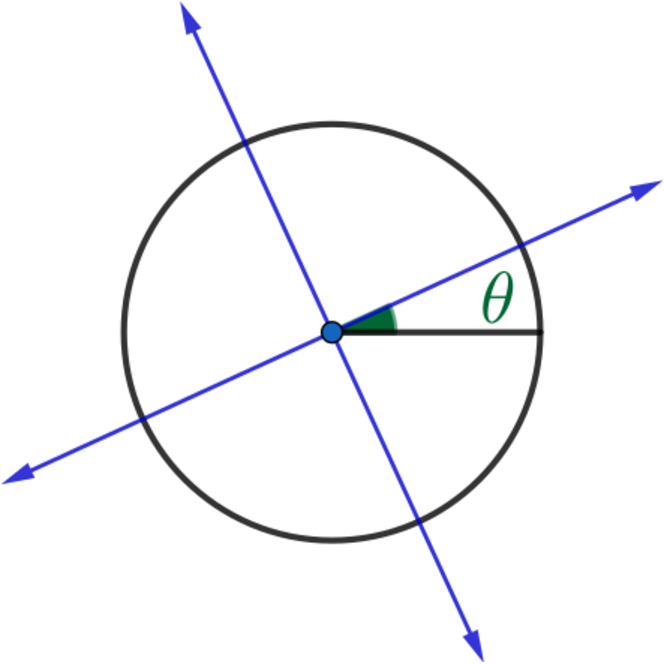
\includegraphics[scale=0.5]{images/cross.pdf}
  \caption{Illustration d'une croix.}
  \label{fig:croix}
\end{figure}

Un champ de croix $\bar{u}$ défini sur $\Omega$ est une fonction qui associe à chaque point $p\in\Omega$ une croix $\bar{u}(p)\in\mathbf{C}$.

\begin{definition}
    Si $\bar{u}(p)=0$ pour $p\in\Omega$ alors on dit que $p$ est un \emph{point singulier} de $\bar{u}$.
\end{definition}

Dans toute la suite, nous désignerons par  $\mathcal{S}_{\bar{u}}:={\bar{u}}^{-1}(\{0\})$ l'ensemble des points singuliers de $\bar{u}$.

\begin{definition}%[ $\mathcal{C}^1$ cross field]
\label{def:cont}
$\bar{u}$ est de classe $\mathcal{C}^1$ en un point $p$ s'il existe une application $\pi_{\bar{u}}$ dans un voisinnage $V_p$ de $p$ tel que $\pi_{\bar{u}}\in\mathcal{C}^1(V_p)$ et $\pi_{\bar{u}}(q)\in\bar{u}(q)$ pour tout $q\in V_p$.
\end{definition}

Comme toutes les composantes de $\bar{u}$ sont obtenues par rotations d'angles $m\pi/2$, où $m\in\mathbb{Z}$, la propriété énoncée précédemment peut être reformulée en tant qu'exigence de continuité $C^1$ pour toutes les composantes dans le voisinage de $p$.

\begin{definition}
    $\bar{u}$ est un champ de croix \emph{presque-$\mathcal{C}^1$} si $\#\mathcal{S}_{\bar{u}}<\infty$ et si $\bar{u}$ est de classe $\mathcal{C}^1$ en tout point $p\in\Omega\backslash\mathcal{S}_{\bar{u}}$.
\end{definition}


Le résultat suivant établit la régularité des champs de croix construits à partir de fonctions de représentation \cite{kowalski2013pde, viertel2019approach} puis définit l'opération et la régularité de la rotation d'un champ de croix par rapport à un champ d'angle (voir figure \ref{fig:repr_to_cross} et figure \ref{fig:rot_cross}).

\begin{proposition}
\label{prop:cont1}
\[\]
\vspace{-1cm}
\begin{enumerate}
\item Soit $f : \Omega \rightarrow \mathbb{R}^2$ un champ de vecteur de classe $\mathcal{C}^1$ sauf en un nombre fini de point où $f$ s'annule. La fonction $\bar{u}$ définie pour tout $p\in\Omega$ par :
\begin{equation}
    \bar{u}(p) =
\left\{
    \begin{array}{lc}
        \displaystyle\left\{\mathbf{R}\left(\frac{m\pi}{2}\right)\frac{f(p)}{\left\|f(p)\right\|},~ m\in \mathbb{Z}\right\} &\text{ si }f(p)\neq 0,\\\\
        0& \text{sinon}
    \end{array}
\right.
\label{eq:repr_to_cross}
\end{equation}
est un champ de croix presque-$\mathcal{C}^1$ sur $\Omega$.

\item Soit $\bar{u}$ un champ de croix sur $\Omega$ et $\theta : \Omega \rightarrow \mathbb{R}$ une fonction définie sur $\Omega$. Alors l'application $\bar{v}:p\mapsto \bar{v}(p)=\mathbf{R}(\theta(p))\bar{u}(p):=\{\mathbf{R}(\theta(p)) u,~u\in \bar{u}(p)\}$ est un champ de croix sur $\Omega$. De plus, $\mathcal{S}_{\bar{u}}=\mathcal{S}_{\bar{v}}$, et si $\theta$ est de classe $\mathcal{C}^1$ alors $\bar{u}$ est de classe $\mathcal{C}^1$ en $p\in \Omega$ (respectivement presque-$\mathcal{C}^1$ sur $\Omega$) si et seulement si $\bar{v}$ l'est.
\end{enumerate}
\end{proposition}

\begin{proof}
\[\]
\vspace{-1cm}
\begin{enumerate}
\item Pour tout $p\in\Omega$, si $\bar{u}(p)\neq 0$ alors pour tout $(u^1, u^2)\in\bar{u}(p)\times\bar{u}(p)$, il existe $m_1,m_2\in\mathbb{Z}$ tel que $u_1=\mathbf{R}(\frac{m_1\pi}{2})\frac{f(p)}{\left\|f(p)\right\|}$ et $u_2=\mathbf{R}(\frac{m_2\pi}{2})\frac{f(p)}{\left\|f(p)\right\|}$. On a donc $u^1=\mathbf{R}(\frac{(m_1-m_2)\pi}{2})u^2$ ce qui implique que $\bar{u}(p)\in\mathbf{C}\backslash\{0\}$. Autrement, $\bar{u}(p)=0$. Il vient donc que $\bar{u}$ est un champ de croix.

Soit $F$ l'ensemble des points où $f$ s'annule. L'application $\pi_{\bar{u}}:=f/\|f\|^{-1}$ définie sur $\Omega\backslash F$ est de classe $\mathcal{C}^1$ puisque $f$ l'est. De plus, pour tout $p\in\Omega\backslash F$, $\pi_{\bar{u}}(p)\in\bar{u}(p)$ donc $\bar{u}$ est de classe $\mathcal{C}^1$ sur $\Omega\backslash F$. Par définition, $\mathcal{S}_{\bar{u}}=F$ donc $\bar{u}$ est un champ de croix presque-$\mathcal{C}^1$ sur $\Omega$.\\

\item Soit $p\in\Omega$. Si $\bar{u}(p)=0$ alors $\bar{v}(p)=0$ sinon $\bar{u}(p)\in\mathbf{C}\backslash\{0\}$ ce qui implique que $\bar{v}(p)\in\mathbf{C}\backslash\{0\}$. En effet, soit $(v^1, v^2)\in\bar{v}(p)\times\bar{v}(p)$. Par définition, il existe $(u^1, u^2)\in\bar{u}(p)\times\bar{u}(p)$ tel que $v^1=\mathbf{R}(\theta)u^1$ et $v^2=\mathbf{R}(\theta)u^2$. Or $\bar{u}(p)\in\mathbf{C}\backslash\{0\}$, donc il existe $m\in\mathbb{Z}$ tel que:
$$
u^1=\mathbf{R}\left(\frac{m\pi}{2}\right)u^2\Longrightarrow
\mathbf{R}(\theta)u^1=\mathbf{R}(\theta)\mathbf{R}\left(\frac{m\pi}{2}\right)u^2\Longrightarrow
v^1=\mathbf{R}\left(\frac{m\pi}{2}\right)v^2.
$$
Ce qui implique que $\bar{v}(p)\in\mathbf{C}\backslash\{0\}$. Autrement dit, $\bar{v}$ est un champ de croix sur $\Omega$. De plus $\mathcal{S}_{\bar{u}}=\mathcal{S}_{\bar{v}}$ puisque pour tout $p\in\Omega$, on a:
$$\bar{v}(p)=\{0\} \Leftrightarrow \left(\forall u\in \bar{u}(p),~\mathbf{R}(\theta(p)) u=0\right)\Leftrightarrow \left(\forall u\in \bar{u}(p),~u=0\right) \Leftrightarrow \bar{u}(p)=\{0\}.$$
Maintenant considérons que $\theta$  et $\bar{u}$ soient de classe $\mathcal{C}^1$ et soit $p\in\Omega$. Par définition, il existe une application $\pi_{\bar{u}}$ de classe $\mathcal{C}^1$ dans un voisinnage $V_p$ de $p$. $\theta$ étant de classe $\mathcal{C}^1$, l'application $\pi_{\bar{v}}:=\mathbf{R}(\theta)\pi_{\bar{u}}$ est de classe $\mathcal{C}^1$ sur $V_p$. De plus, pour tout $q\in V_p$, $\pi_{\bar{v}}(q)=\mathbf{R}(\theta(q))\pi_{\bar{u}}(q)$ et comme $\pi_{\bar{u}}(q)\in\bar{u}(q)$ on a par définition $\pi_{\bar{v}}(q)\in\bar{v}(q)$. En conclusion, $\bar{v}$ est de classe $\mathcal{C}^1$ sur $\Omega$. Réciproquement, si $\bar{v}$ est de classe $\mathcal{C}^1$ sur $\Omega$, alors par définition il existe une application $\pi_{\bar{v}}$ de classe $\mathcal{C}^1$ dans un voisinnage $V_p$ de $p$. $\theta$ étant de classe $\mathcal{C}^1$, l'application $\pi_{\bar{u}}:=\mathbf{R}(-\theta)\pi_{\bar{v}}$ est de classe $\mathcal{C}^1$ sur $V_p$. De plus, pour tout $q\in V_p$, $\pi_{\bar{u}}(q)=\mathbf{R}(-\theta(q))\pi_{\bar{v}}(q)$. Or $\pi_{\bar{v}}(q)\in\bar{v}(q)$ donc par définition il existe $u\in\bar{u}(q)$ tel que $\pi_{\bar{v}}(q)=\mathbf{R}(\theta(q))u$. On a donc :
$$
\pi_{\bar{u}}(q)=\mathbf{R}(-\theta(q))\mathbf{R}(\theta(q))u=u\Longrightarrow\pi_{\bar{u}}\in\bar{u}(q).
$$
En conclusion, $\bar{v}$ est de classe $\mathcal{C}^1$ sur $\Omega$. Pour finir, puisque $\mathcal{S}_{\bar{u}}=\mathcal{S}_{\bar{v}}$ alors $\bar{u}$ est un champ de croix presque-$\mathcal{C}^1$ si et seulement si $\bar{v}$ est un champ de croix presque-$\mathcal{C}^1$.
\end{enumerate}
\end{proof}

\begin{figure}[!h]
  \centering
  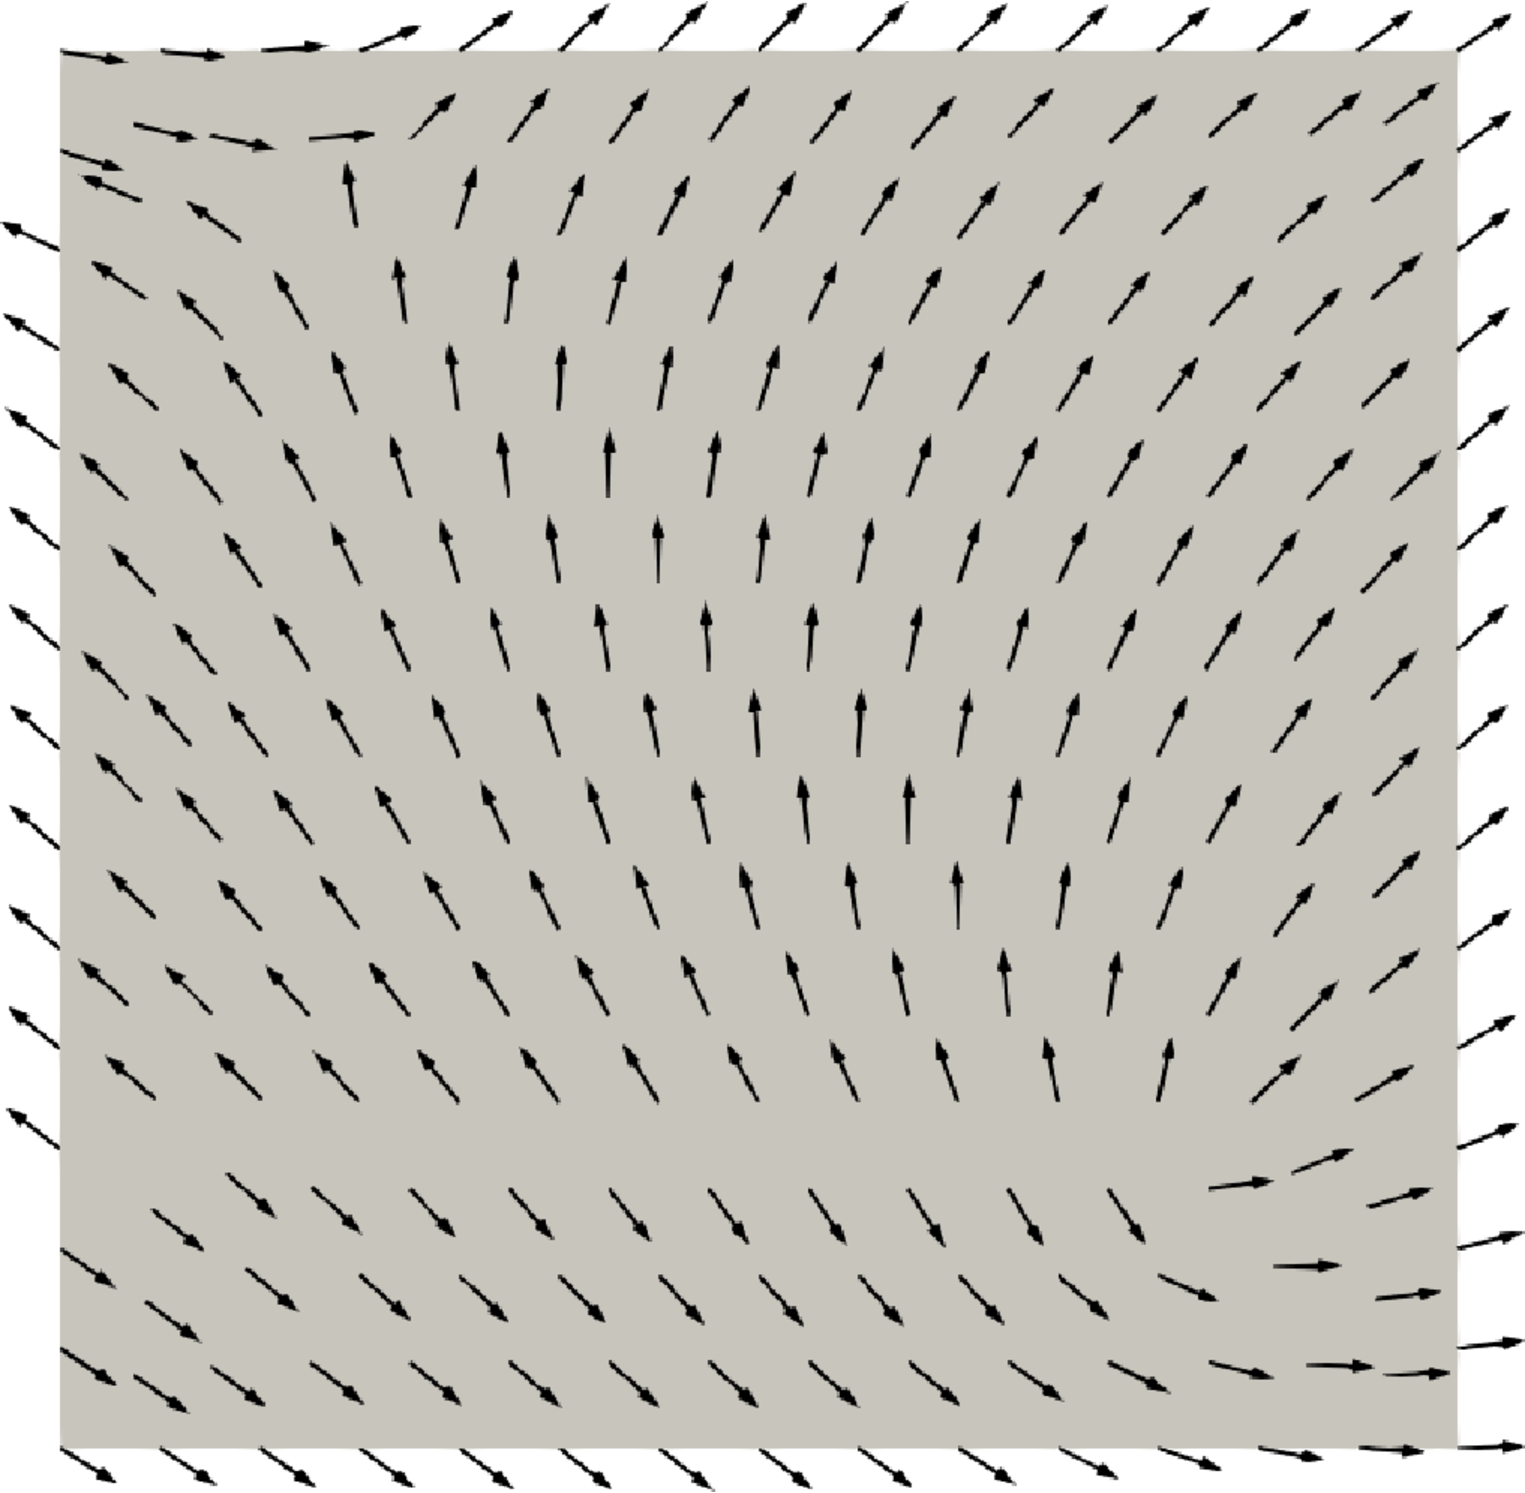
\includegraphics[scale=0.28]{images/repre_field.pdf}\hspace{0.5cm}
  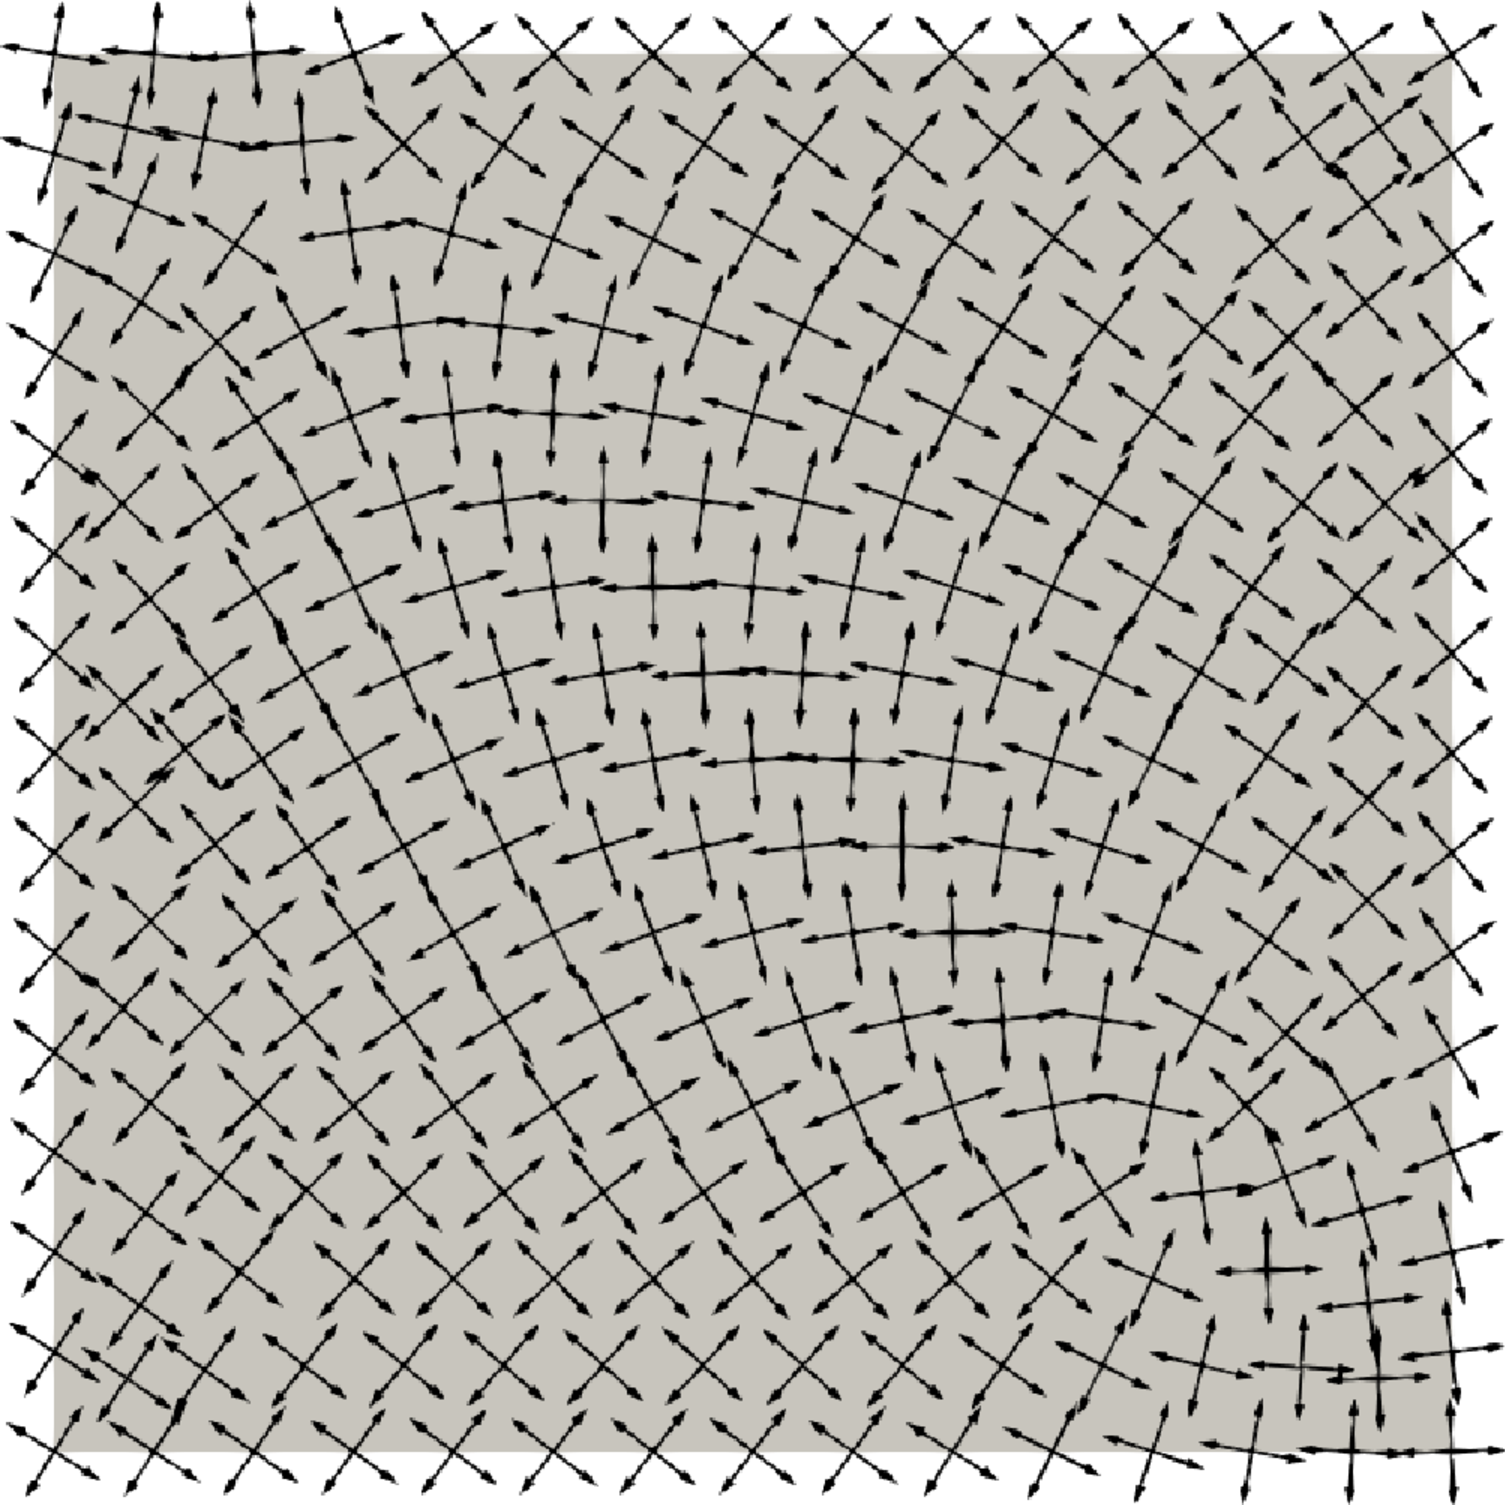
\includegraphics[scale=0.28]{images/cross_from_repre_field.pdf}
  \caption{Illustration d'un champ de représentation (en gauche) et du champ de croix associé (à droite).}
  \label{fig:repr_to_cross}
\end{figure}

\begin{figure}[!h]
  \centering
  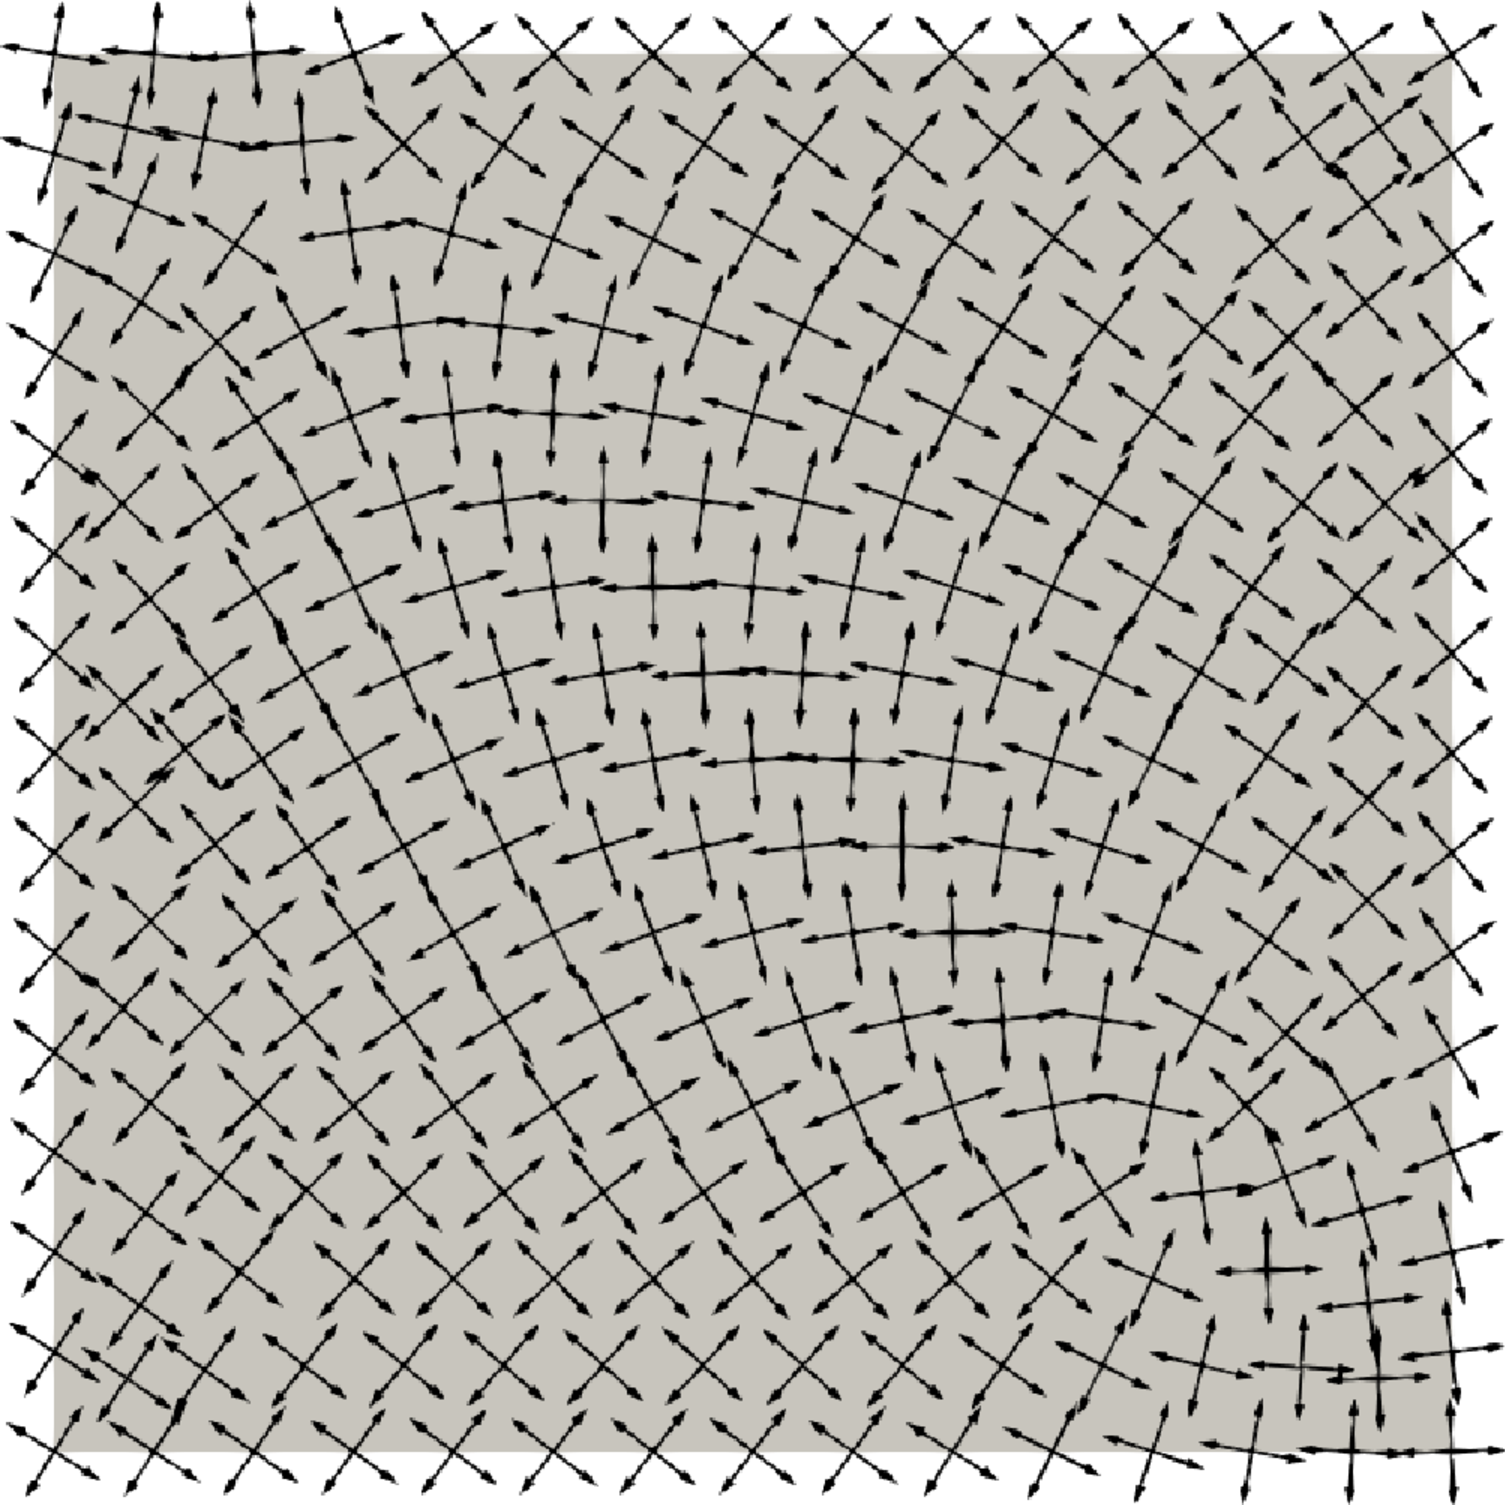
\includegraphics[scale=0.18]{images/cross_from_repre_field.pdf}\hspace{0.5cm}
  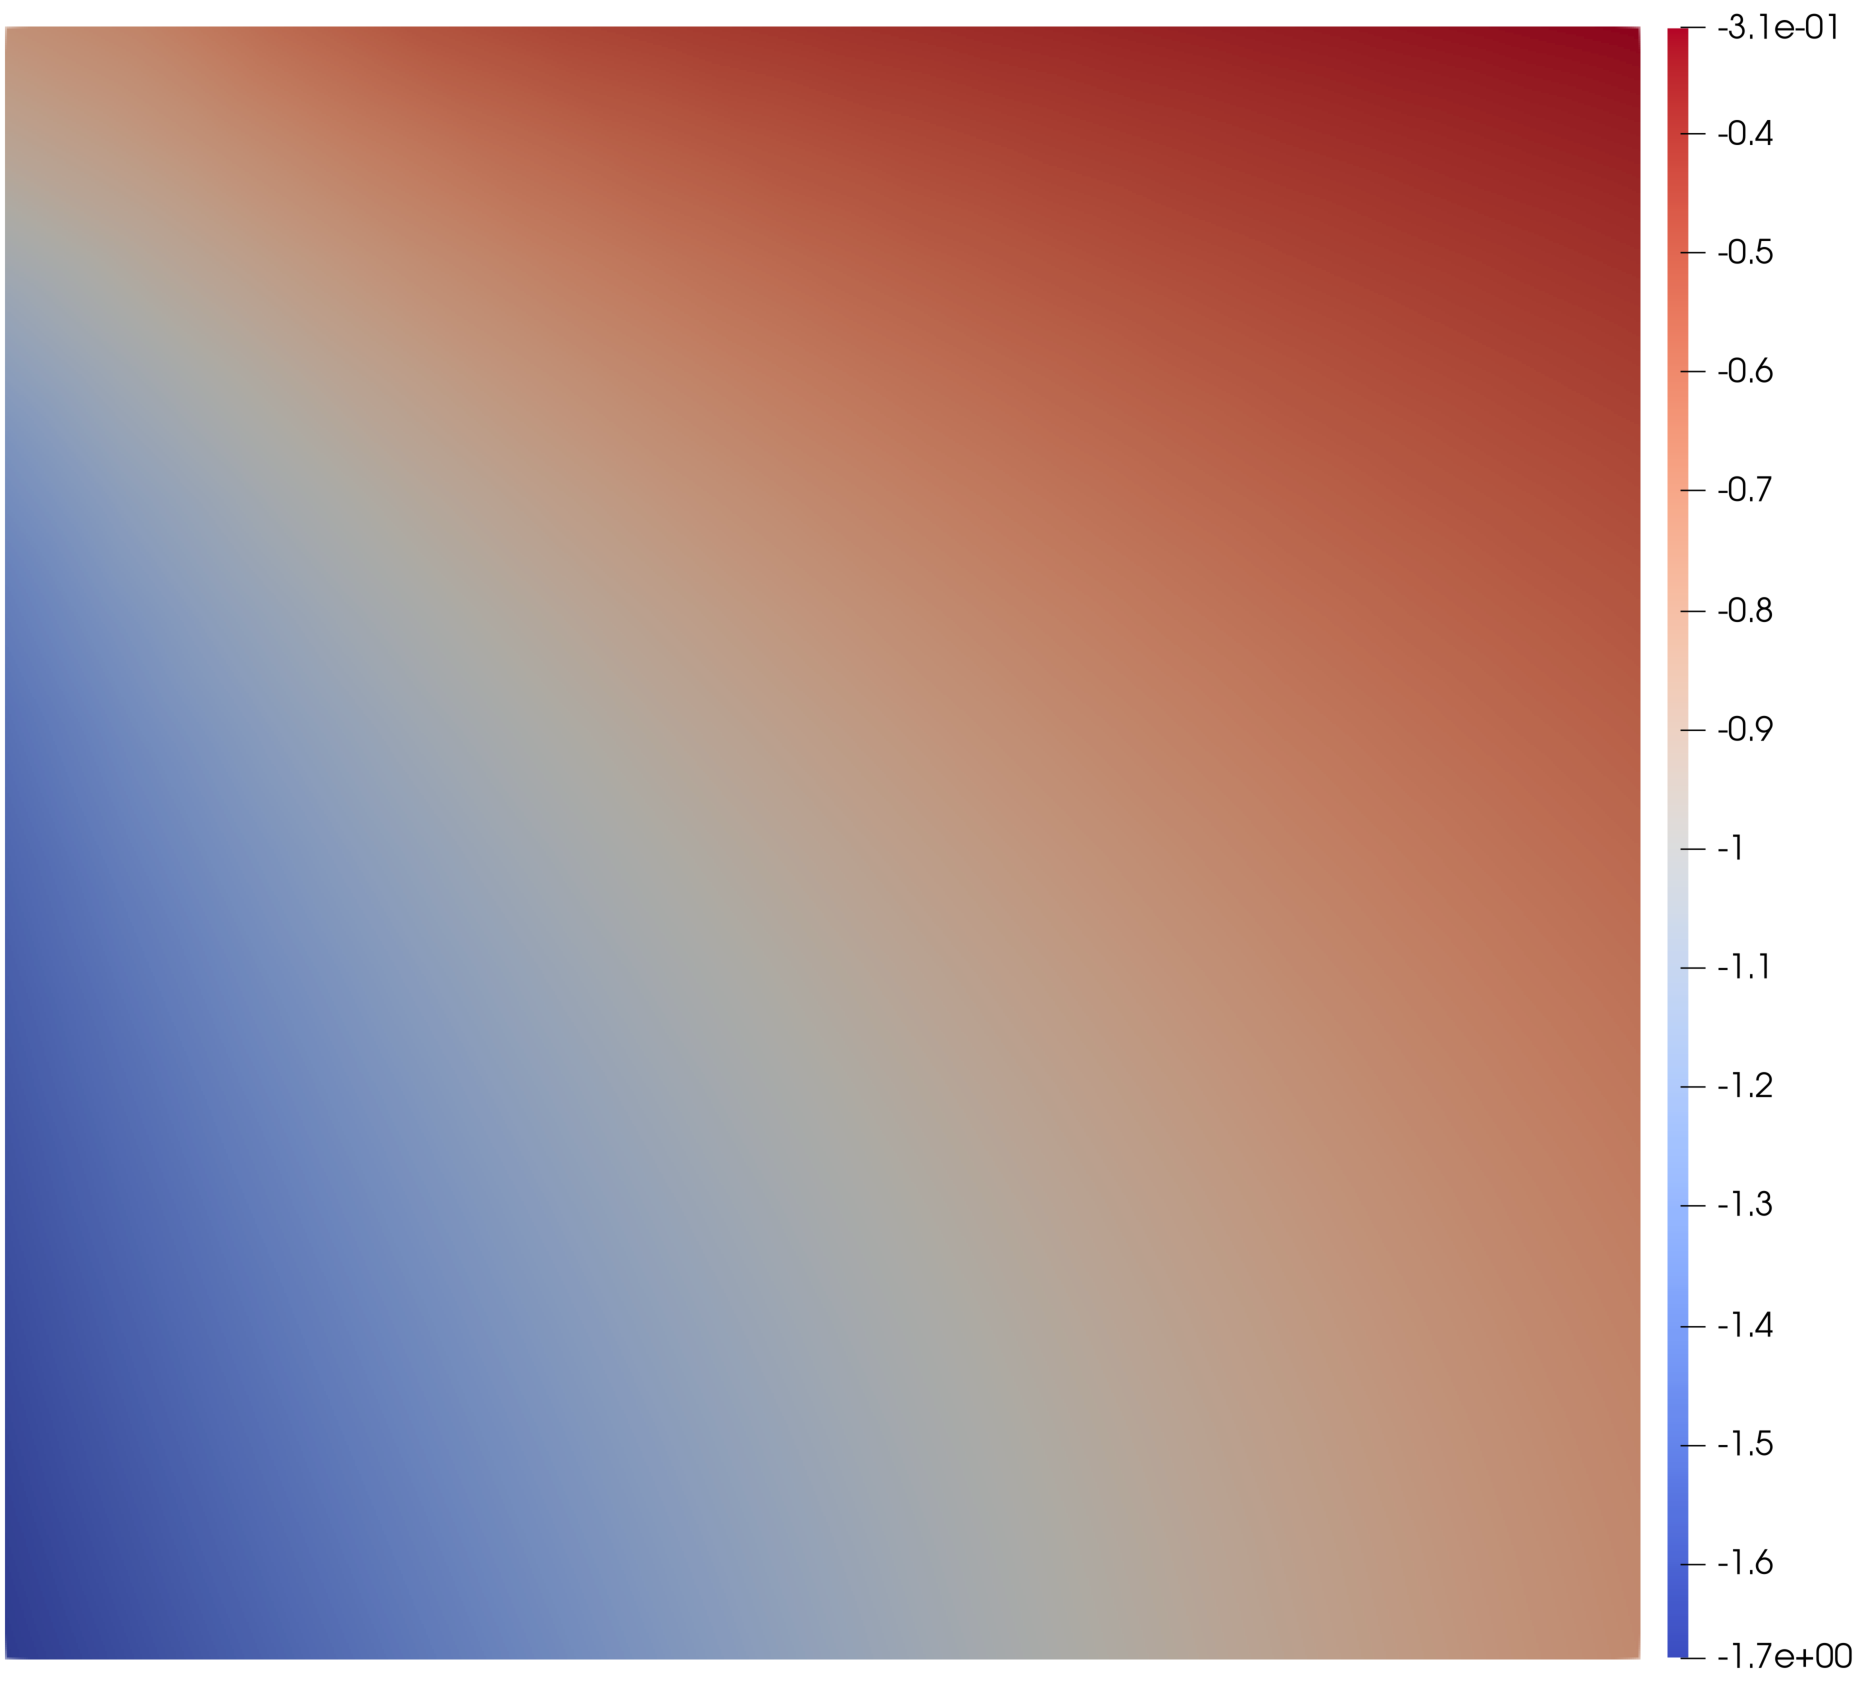
\includegraphics[scale=0.188]{images/scal_field.pdf}\hspace{0.5cm}
  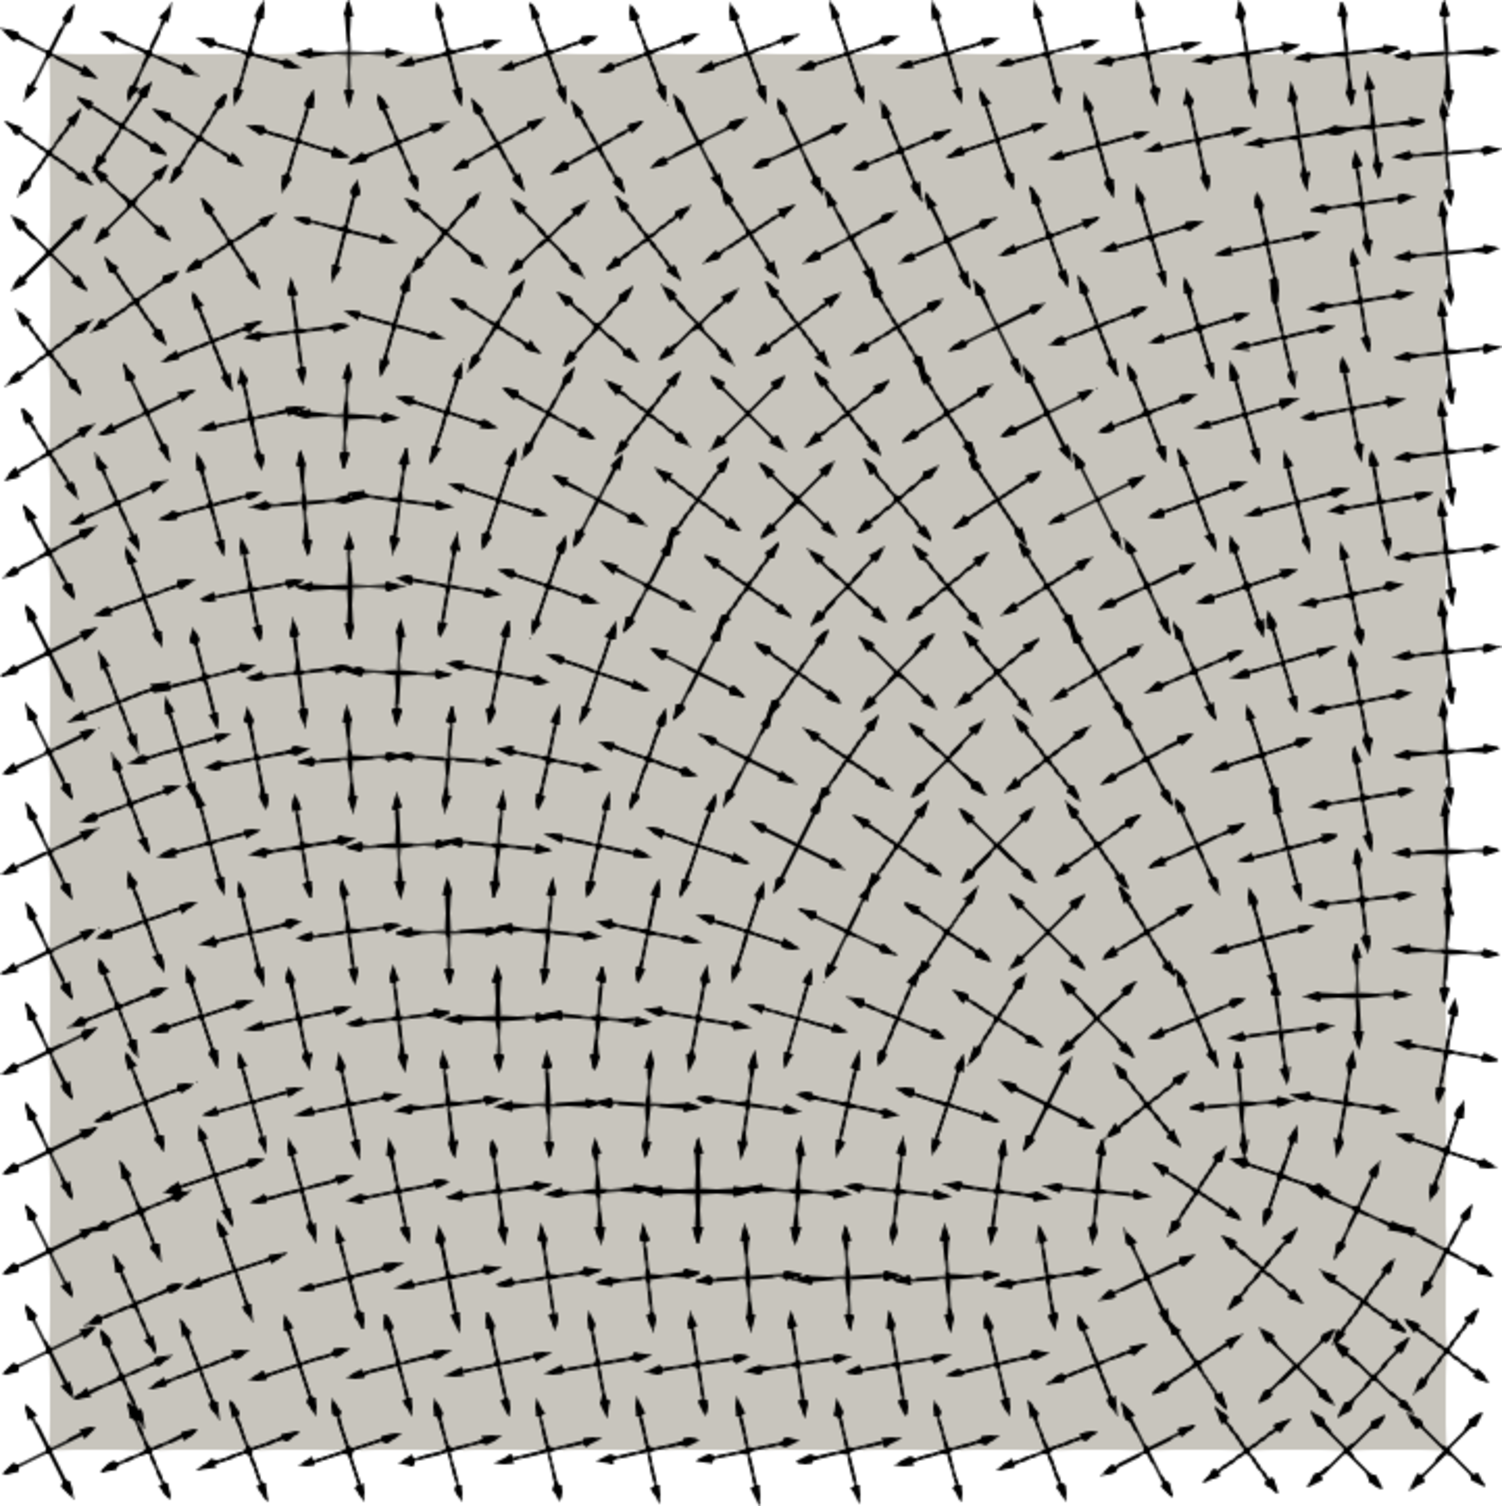
\includegraphics[scale=0.18]{images/result_field.pdf}
  \caption{Illustration de la rotation d'un champ de croix par rapport à un champ d'angle sur un domaine quelconque. \'A gauche : champ de croix initial, au milieu: champ d'angle (en radian), à droite: champ de croix résultant.}
  \label{fig:rot_cross}
\end{figure}

Pour tout point $p$ situé sur la frontière $\partial\Omega$, nous définissons $N(p)$ comme étant la normale extérieure unitaire. Lorsque la normale n'est pas définie en $p$, nous posons $N(p)=(0,0)$. En accord avec la proposition \ref{prop:cont1}, nous introduisons un champ de croix particulier associé à la frontière de $\Omega$, dite \emph{champ de croix normal} et définit par:
\begin{equation}
    \bar{N}(p) =
\left\{
    \begin{array}{ll}
        \left\{\mathbf{R}\left(\frac{m\pi}{2}\right)N(p),~ m\in \mathbb{Z}\right\} &\text{ si }N(p)\neq (0,0),\\\\
        0& \text{ sinon }.
    \end{array}
\right.
\end{equation}
Nous pouvons alors introduire la notion d'alignement du champ de croix par la définition suivante:
\begin{definition}
    Le champ de croix $\bar{u}$ est dit aligné par rapport à $\partial\Omega$ ou aligné sur le bord de $\Omega$ si pour tout point $p\in\partial\Omega$, $\bar{u}(p)\in\{\bar{N}(p), 0\}$.
\end{definition}

\subsection{Indice}

L'indice de Poincaré est un concept mathématique profondément enraciné dans la topologie et la géométrie différentielle. Elle permet de quantifier le comportement des courbes et des champs de vecteurs à travers leurs singularités. Dans cette partie, à l'instar du concept d'indices pour les champs de vecteurs, nous introduisons un indice spécifique pour les champs de croix. Ces indices seront plus tard relié à la notion de \emph{séparatrices}.

Pour commencer, nous définissons la notion d'angle pour une croix. À chaque croix, nous associons une représentation angulaire. Cette approche consiste à attribuer à la croix une valeur représentant son orientation par rapport à une référence donnée.

\begin{definition}
    \label{def:cross_angle}
    Soit une croix $\mathbf{c}\in\mathbf{C}\backslash\{0\}$. L'angle associé à $\mathbf{c}$ est donné par l'unique élément de l'ensemble:
    %$$\left\{\theta_{\bar{u}}\right\} :=
    $$\{\theta_{\mathbf{c}}\} := \left\{\arg c,~c\in \mathbf{c}\right\} \cap \left]-\frac{\pi}{4},\frac{\pi}{4}\right],$$
    où $\arg c\equiv atan2(c_y, c_x)\pmod{2\pi}$ est l'argument complexe de $c=(c_x, x_y)$ pour tout $c\in\mathbf{c}$.
\end{definition}

\begin{lemma}
    L'angle donné par la définition \ref{def:cross_angle} est bien défini.
\end{lemma}

\begin{proof}
    Existence: L'ensemble $\left\{\arg c,~c\in \mathbf{c}\right\} \cap \left]-\frac{\pi}{4},\frac{\pi}{4}\right]$ est non vide. En effet, si $\left\{\arg c,~c\in \mathbf{c}\right\} \cap \left]-\frac{\pi}{4},\frac{\pi}{4}\right]=\emptyset$, alors $\left\{\arg c,~c\in \mathbf{c}\right\}=\emptyset$. Autrement dit, $\mathbf{c}=0$ ce qui est exclut.\\
    Unicité: Supposons que $\mathbf{c}$ ait deux angles $\theta_{\mathbf{c}}$ et $\theta^{'}_{\mathbf{c}}$. Par définition il existe $m, n\in\mathbb{Z}$ et $c,c^{'}\in\mathbf{c}$ tel que:
    $$
    \theta_{\mathbf{c}}-\theta^{'}_{\mathbf{c}}=atan2(c_y, c_x)+2m\pi-atan2(c^{'}_y, c^{'}_x)-2n\pi.
    $$
    De plus, il existe $l\in\mathbb{Z}$ tel que:
    $$
    atan2(c^{'}_y,c^{'}_x)=atan2(c_y,c_x)+l\frac{\pi}{2}.
    $$
    On a donc:
    $$
    \theta_{\mathbf{c}}-\theta^{'}_{\mathbf{c}}=2m\pi-2n\pi-l\frac{\pi}{2}=k\frac{\pi}{2},
    $$
    où $k=4m-4n-l$.
    Sachant que $\theta_{\mathbf{c}},\theta_{\mathbf{c}}^{'}\in\left]-\frac{\pi}{4},\frac{\pi}{4}\right]$, on a $\theta_{\mathbf{c}}-\theta^{'}_{\mathbf{c}}\in\left]-\frac{\pi}{2},\frac{\pi}{2}\right[$ ce qui implique que:
    $$
    -\frac{\pi}{2}<k\frac{\pi}{2}<\frac{\pi}{2}.
    $$
    Il vient donc que $k=0$ puisque $k\in\mathbb{Z}$. Autrement dit, $\theta_{\mathbf{c}}=\theta_{\mathbf{c}}^{'}$.
\end{proof}

%Comme dans \cite{beaufort2017computing}, $\Theta$ peut être vue comme l'angle minimum des vecteurs composant la croix $\mathbf{c}$.

En considérant un champ de croix $\bar{u}$, la définition précédente nous autorise à attribuer à $\bar{u}$ un champ scalaire formé par les angles des croix de $\bar{u}$. Ce champ est défini de la manière suivante :

\begin{definition}
    Soit $\bar{u}$ un champ de croix presque-$\mathcal{C}^1$ sur $\Omega$. Le champ d'angle associé à $\bar{u}$ est l'application définie par:
    $$\theta_{\bar{u}}:p\in\Omega\backslash\mathcal{S}_{\bar{u}}\longmapsto\theta_{\bar{u}}(p):=\theta_{\bar{u}(p)},$$
    où $\theta_{\bar{u}(p)}$ est l'angle de la croix $\bar{u}(p)$ donné par la définition \ref{def:cross_angle}.
\end{definition}

\begin{figure}[!h]
  \centering
  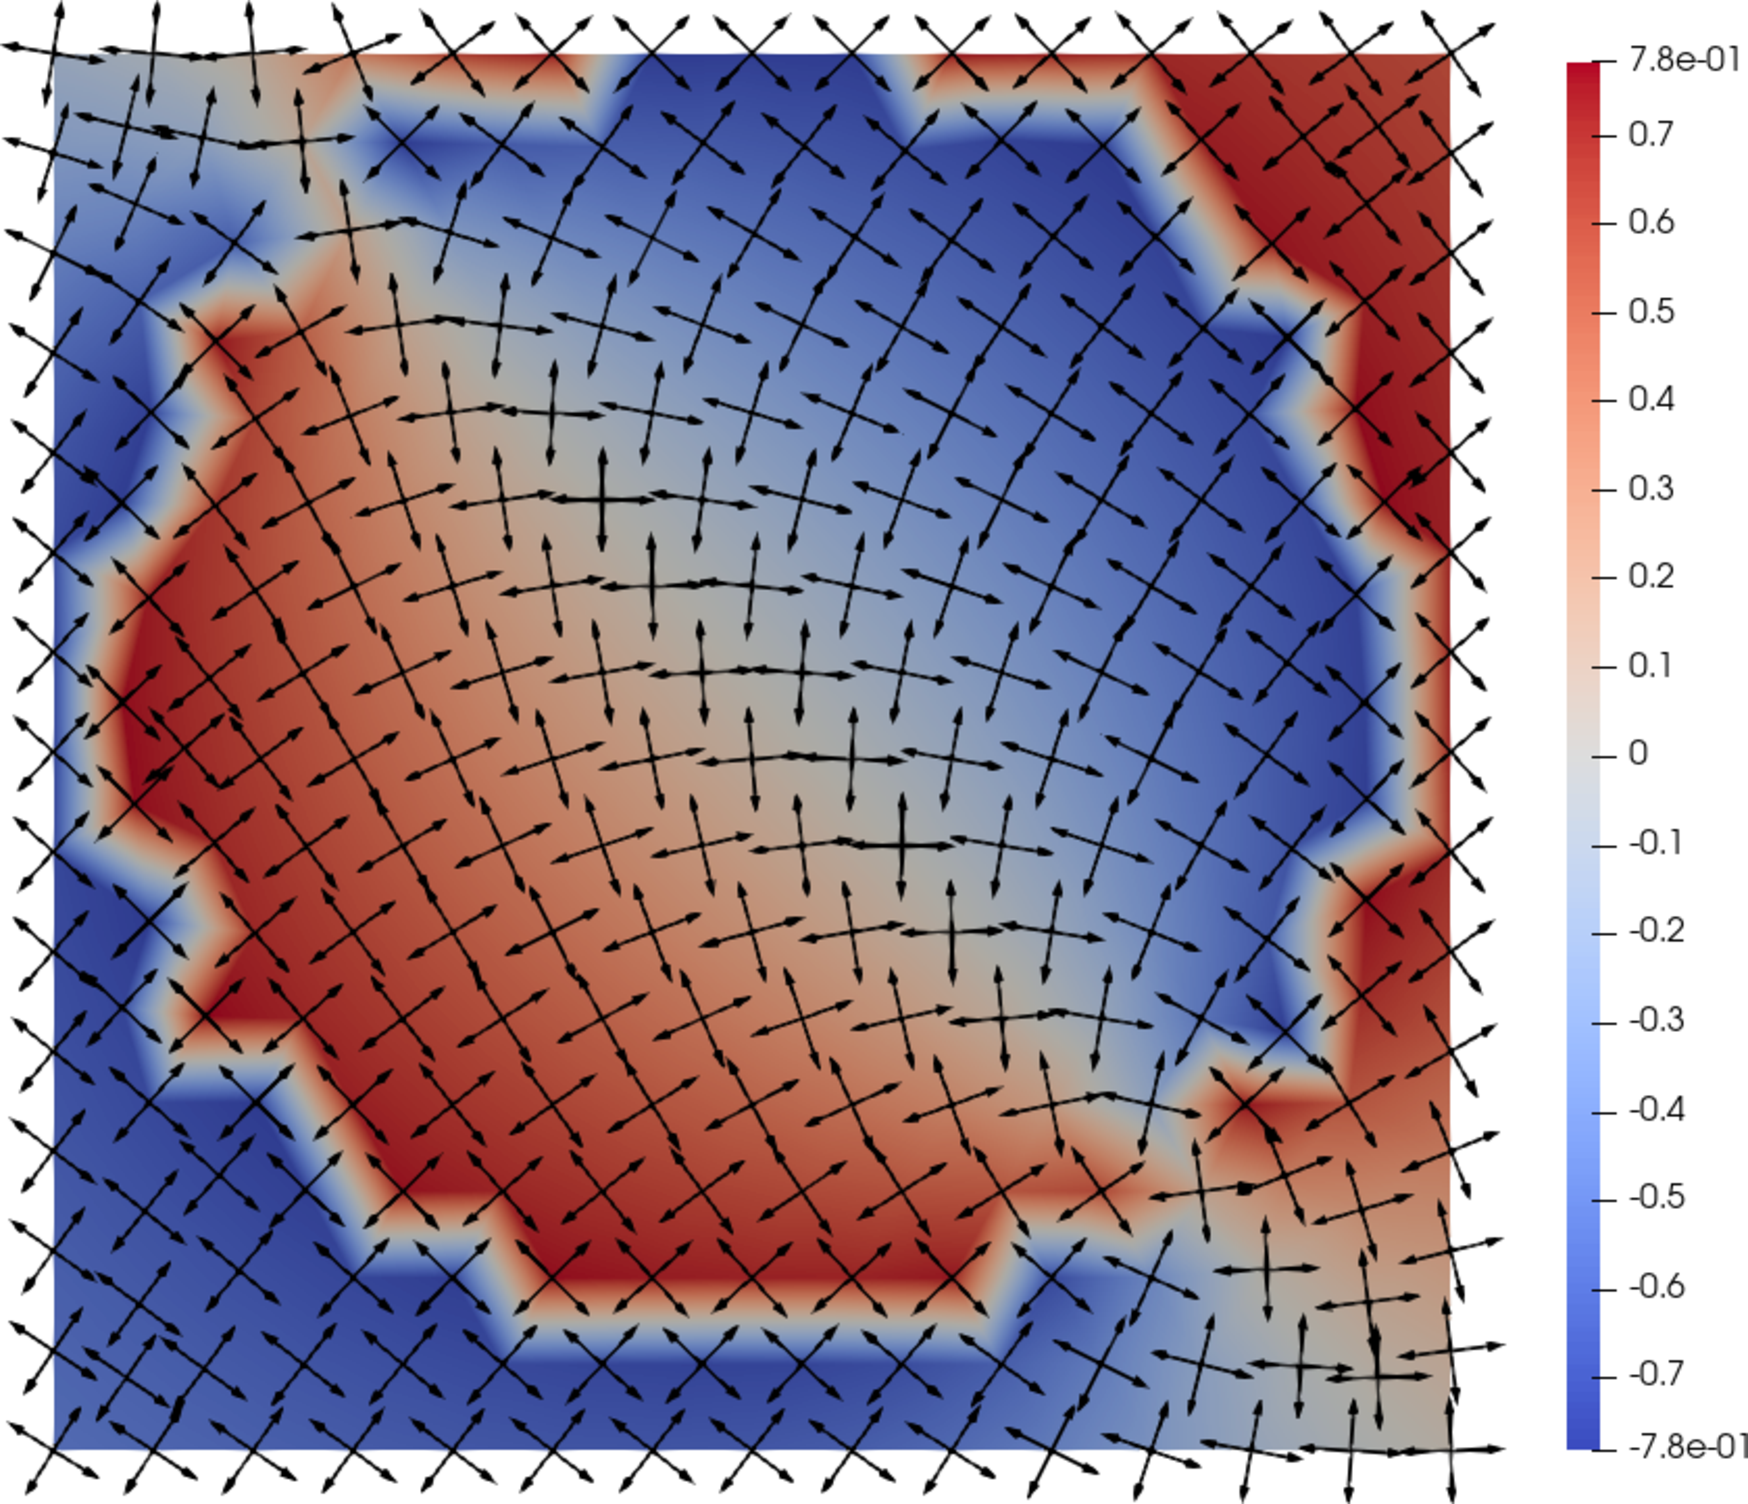
\includegraphics[scale=0.32]{images/cross_ang_field.pdf}
  \caption{Illustration d'un champ de croix et du champ d'angle (en radian) correspondant.}
  \label{fig:cross_field}
\end{figure}


Nous énonçons à présent le résultat suivant, qui constitue un outil précieux pour analyser la régularité d'un champ de croix donné à partir de la régularité du champ d'angle qui lui est associé.

\begin{proposition}
    \label{prop:angular_cont}
    Soit $\bar{u}$ un champ de croix sur $\Omega$. $\bar{u}$ est de classe $\mathcal{C}^1$ en un point $p\in\Omega$ si et seulement s'il existe $V_p\subset \Omega \backslash \mathcal{S}_{\bar{u}}$, un voisinage de $p$, et une fonction $\theta_{\bar{u}}^{V_p}:V_p \rightarrow \mathbb{R}$ telle que $\theta_{\bar{u}}^{V_p}\in \mathcal{C}^1(V_p)$ et vérifiant $\theta_{\bar{u}}^{V_p}(q)\equiv\theta_{\bar{u}}(q) \pmod{\frac{\pi}{2}}$, pour tout $q\in V_p$.
\end{proposition}


\begin{proof}
    Supposons que $\bar{u}$ est de classe $\mathcal{C}^1$ en un point $p\in\Omega$. Par définition, il existe une application $\pi_{\bar{u}}$ de classe $\mathcal{C}^1$ dans un voisinage $V_p$ de $p$. Par conséquent, la fonction $\theta_{\bar{u}}^{V_p}:=\arg \pi_{\bar{u}}$ est de classe $\mathcal{C}^1$ dans $V_p$. De plus, pour tout $q\in V_p$, $\pi_u(q)\in\bar{u}(q)$ autrement dit, pour tout $q\in V_p$, il existe $m\in\mathbb{Z}$ tel que $\arg\pi_{\bar{u}}(q)=\theta_{\bar{u}}(q)+m\frac{\pi}{2}$. On en déduit que $\theta_{\bar{u}}^{V_p}$ vérifie $\theta^{V_p}_{\bar{u}}(q)\equiv\theta_{\bar{u}}(q)\pmod{\frac{\pi}{2}}$ pour tout $q\in V_p$.

    Réciproquement, supposons qu'il existe $V_p\subset \Omega \backslash \mathcal{S}_{\bar{u}}$, un voisinage de $p$, et une fonction $\theta_{\bar{u}}^{V_p}:V_p \rightarrow \mathbb{R}$ telle que $\theta_{\bar{u}}^{V_p}\in \mathcal{C}^1(V_p)$ et vérifiant $\theta_{\bar{u}}^{V_p}(q)\equiv\theta_{\bar{u}}(q) \pmod{\frac{\pi}{2}}$, pour tout $q\in V_p$. Il vient que l'application $\pi_{\bar{u}}:=\mathbf{R}(\theta_{\bar{u}}^V)(1,0)$ est de classe $\mathcal{C}^1$ sur $V_p$. De plus, pour tout $q\in V_p$, $\pi_{\bar{u}}(q)\in \bar{u}(q)$ puisqu'il existe $m\in\mathbb{Z}$ tel que $\arg\pi_{\bar{u}}(q)=\theta_{\bar{u}}(q)+m\frac{\pi}{2}$. Ainsi $\bar{u}$ est de classe $\mathcal{C}^1$ en $p$.
\end{proof}


Grâce au résultat précédent, nous pouvons déduire le corollaire suivant permettant de construire le relèvement continu de l'angle d'un champ de croix le long d'une courbe paramétrée.

\begin{corollary}
    \label{cor:relevement_continu}
    Soit $\gamma: [0, 1] \longrightarrow \Omega$ un arc sur $\Omega$ et $\bar{u}$ un champ de croix presque-$\mathcal{C}^1$ défini sur $\Omega$ tel que pour tout $p\in\gamma([0, 1)$, $\bar{u}(p)\neq 0$. Alors, il existe $\theta^\gamma_{\bar{u}}: [0, 1] \longrightarrow \mathbb{R}$  une fonction de classe $\mathcal{C}^1$ sur $]0,1[$ telle que $\theta^\gamma_{\bar{u}}(t) \equiv \theta_{\bar{u}}(\gamma(t)) \pmod{\frac{\pi}{2}}$. De plus, si $\alpha_{\bar{u}}^\gamma$ et $\beta_{\bar{u}}^\gamma$ sont deux fonctions de classe $\mathcal{C}^1$ satisfaisant cette propriété, alors il existe $m \in \mathbb{Z}$ tel que $\alpha_{\bar{u}}^\gamma(t) = \beta_{\bar{u}}^\gamma(t) + m\frac{\pi}{2}$ pour tout $t \in [0, 1]$.
\end{corollary}

\begin{proof}
    Pour démontrer ce résultat, nous commençons par construire un recouvrement fini de $\gamma$. Nous construisons ensuite $\theta_{\bar{u}}^\gamma$ par morceaux sur les éléments du recouvrement.

    \paragraph{Construction d'un recouvrement de la courbe $\gamma$:} Soit $p\in\gamma([0, 1])$. D'après la proposition \ref{prop:angular_cont}, il existe $V_p\subset\Omega\backslash\mathcal{S}_{\bar{u}}$ et une fonction $\theta_{\bar{u}}^{V_p}\in\mathcal{C}^1$ vérifiant $\theta_{\bar{u}}^{V_p}(q)\equiv\theta_{\bar{u}}(q)\pmod{\frac{\pi}{2}}$ pour tout $q\in V_p$. Notons maintenant $\widetilde{V_p}$ la composante connexe de l'ensemble $V_p\cap\gamma([0, 1])$ et contenant $p$. Il est clair que la famille $(\widetilde{V_p})_{p\in\gamma([0, 1])}$ recouvre $\gamma([0, 1])$ puisque $\displaystyle\cup_{p\in\gamma([0, 1])}\widetilde{V_p}$ contient $\gamma([0, 1])$. $\gamma$ étant continu et $[0, 1]$ étant compact, on peut extraire de ce recouvrement, un sous-recouvrement fini de $\gamma([0, 1])$. Autrement dit, il existe $I\subset\mathbb{N}$ une partie finie de $\mathbb{N}$ et une sous-famille $(V_i)_{i\in I}$ de $(\widetilde{V_p})_{p\in\gamma([0, 1])}$ recouvrant $\gamma([0, 1])$.

    \paragraph{Construction de $\theta_{\bar{u}}^\gamma$ par morceau:} Soit $\{p_0\}=\gamma^{-1}(0)$ et $V_0\in(V_i)_{i\in I}$ tel que $p_0\in V_0$. On définit $\theta_{\bar{u}}^\gamma(t):=\theta_{\bar{u}}^{V_0}\circ\gamma(t)$ pour tout $t\in\gamma^{-1}(V_0\cap\gamma([0, 1]))$. Il est clair que $\theta_{\bar{u}}^\gamma\in\mathcal{C}^1(\gamma^{-1}(V_0\cap\gamma(]0, 1[))$ et $\theta_{\bar{u}}^\gamma(t)\equiv\theta_{\bar{u}}(\gamma(t))\pmod{\frac{\pi}{2}}$ pour tout $t\in\gamma^{-1}(V_0\cap\gamma([0, 1]))$. À partir de là, nous itérons la construction de $\theta^\gamma_{\bar{u}}$ de la manière suivante: pour $n>0$, on choisit le point $p_n$ tel que $p_n\in\partial V_{n-1}\cap\gamma([0, 1])$ et $p_n\notin\{p_0,\dots,p_{n-1}\}$. On choisit ensuite $V_n$ tel que $V_n\in(V_i)_{i\in I}$ et $p_n\in V_n$. D'après la proposition \ref{prop:angular_cont}, il existe $\theta_{\bar{u}}^{V_n}\in\mathcal{C}^1(V_n)$ et pour tout $q\in V_n$, $\theta_{\bar{u}}^{V_n}(q)\equiv\theta_{\bar{u}}(q)\pmod{\frac{\pi}{2}}$. Soit $m\in\mathbb{Z}$ tel que $\theta^{V_n}_{\bar{u}}\circ\gamma(t)+m\frac{\pi}{2}=\theta^\gamma_{\bar{u}}(t)$ pour tout $t\in\gamma^{-1}(V_{n-1}\cap\gamma([0, 1]))\cap\gamma^{-1}(V_n\cap\gamma([0, 1]))$. On définit alors $\theta_{\bar{u}}^\gamma(t):=\theta^{V_n}_{\bar{u}}\circ\gamma(t)+m\frac{\pi}{2}$ pour tout $t\in\gamma^{-1}(V_n\cap\gamma([0, 1)])$. Il est clair que $\theta_{\bar{u}}^\gamma$ ainsi définit est de classe $\mathcal{C}^1$ sur $\cup_{k=0}^n\gamma^{-1}(V_k\cap\gamma(]0, 1[))$ et $\theta_{\bar{u}}^\gamma(t)\equiv\theta_{\bar{u}}\circ\gamma(t)\pmod{\frac{\pi}{2}}$ pour tout $t\in\cup_{k=0}^n\gamma^{-1}(V_k\cap\gamma([0, 1]))$. On poursuit itérativement cette construction jusqu'à ce que $\cup_{k=0}^n\gamma^{-1}(V_k\cap\gamma([0, 1]))=\gamma([0, 1])$. Le nombre d'itération à faire est finie puisque $(V_i)_{i\in I}$ est un recouvrement fini de $\gamma([0, 1])$.
    \[\]
    Supposons maintenant que $\alpha_{\bar{u}}^\gamma$ et $\beta_{\bar{u}}^\gamma$ sont deux fonctions de classe $\mathcal{C}^1$ qui satisfont cette propriété, alors, il existe des fonctions $g:[0, 1]\longrightarrow\mathbb{Z}$ et $h:[0, 1]\longrightarrow\mathbb{Z}$ telles que $\alpha^\gamma_{\bar{u}}(t) = \theta_{\bar{u}}(\gamma(t)) + g(t)\frac{\pi}{2}$ et $\beta^\gamma_{\bar{u}}(t) =\theta_{\bar{u}}(\gamma(t)) + h(t)\frac{\pi}{2}$. Par conséquent, pour tout $t\in[0, 1]$ on a:
    $$\alpha_{\bar{u}}^\gamma(t) = \beta_{\bar{u}}^\gamma(t) + g(t)\frac{\pi}{2}-h(t)\frac{\pi}{2}.$$
    $\alpha^\gamma_{\bar{u}}$ et $\beta^\gamma_{\bar{u}}$ étant continue sur $[0, 1]$, il vient que la fonction $g-h$ est continue sur $[0, 1]$. Autrement dit, $g-h$ est constant. Soit $m\in\mathbb{Z}$ tel que $m=(g-h)(t)$, pour tout $t\in[0, 1]$, On a:
    $$\forall t\in[0, 1],\quad\alpha_{\bar{u}}^\gamma(t) = \beta_{\bar{u}}^\gamma(t) + m\frac{\pi}{2}.$$
\end{proof}

Le relèvement continu du champ de croix le long d'une courbe paramétrée permet de quantifier le nombre de fois que le champ tourne sur lui-même le long de la courbe. Cependant, la construction du Corollaire \ref{cor:relevement_continu} ne fonctionne pas si $\mathcal{S}_{\bar{u}}\cap\gamma([0,1])\neq\emptyset$. Dans ce cas, nous construisons le relèvement par morceaux le long de $\gamma$ de la manière suivante :

Soit $I:=\gamma^{-1}(\mathcal{S}_{\bar{u}}\cap\gamma([0, 1]))\cup\{0, 1\}$. On a $\#I<\infty$ puisque $\#\mathcal{S}_{\bar{u}}<\infty$. Il existe donc $(t_i)_{i\in\llbracket 1, n_I\rrbracket}\subset[0,1]$ tel que $I=(t_i)_{i\in\llbracket 1, n_I\rrbracket}$ avec $0=t_1<\dots<t_{n_I}=1$ et $n_I=\#I$. Par construction, il est clair que pour tout $i\in\llbracket 1, n_I-1 \rrbracket$, on a $\mathcal{S}_{\bar{u}}\cap\gamma(]t_i, t_{i+1}[)=\emptyset$. Ainsi, à partir du Corollaire \ref{cor:relevement_continu}, nous pouvons construire pour tout $i\in\llbracket 1, n_I-1\rrbracket$ une fonction $\theta^{\gamma_i}_{\bar{u}}$ sur $[0,1]$ et de classe $\mathcal{C}^1$ sur $]0,1[$ telle que $\theta_{\bar{u}}^{\gamma_i}(t)\equiv\theta_{\bar{u}}(\gamma_i(t))\pmod{\frac{\pi}{2}}$ avec $\gamma_i$, l'arc défini sur $[0, 1]$ par :
$$
\forall t\in[0, 1],~\gamma_i(t)=\gamma(t_i+t(t_{i+1}-t_i)).
$$
Finalement, le relèvement $\theta_{\bar{u}}^\gamma$ le long de $\gamma$ est donné par:
\begin{eqnarray*}
    \forall i\in\llbracket 1, n_I\rrbracket,~\forall t\in]t_i, t_{i+1}[,~\theta_{\bar{u}}^\gamma(t)=\theta_{\bar{u}}^{\gamma_i}\left(\frac{t-t_i}{t_{i+1}-t_i}\right).
\end{eqnarray*}



Grâce à cette notion, nous sommes désormais en mesure de définir l'indice d'un point dans un champ de croix.



\begin{comment}
    \begin{figure}[!h]
  \centering
  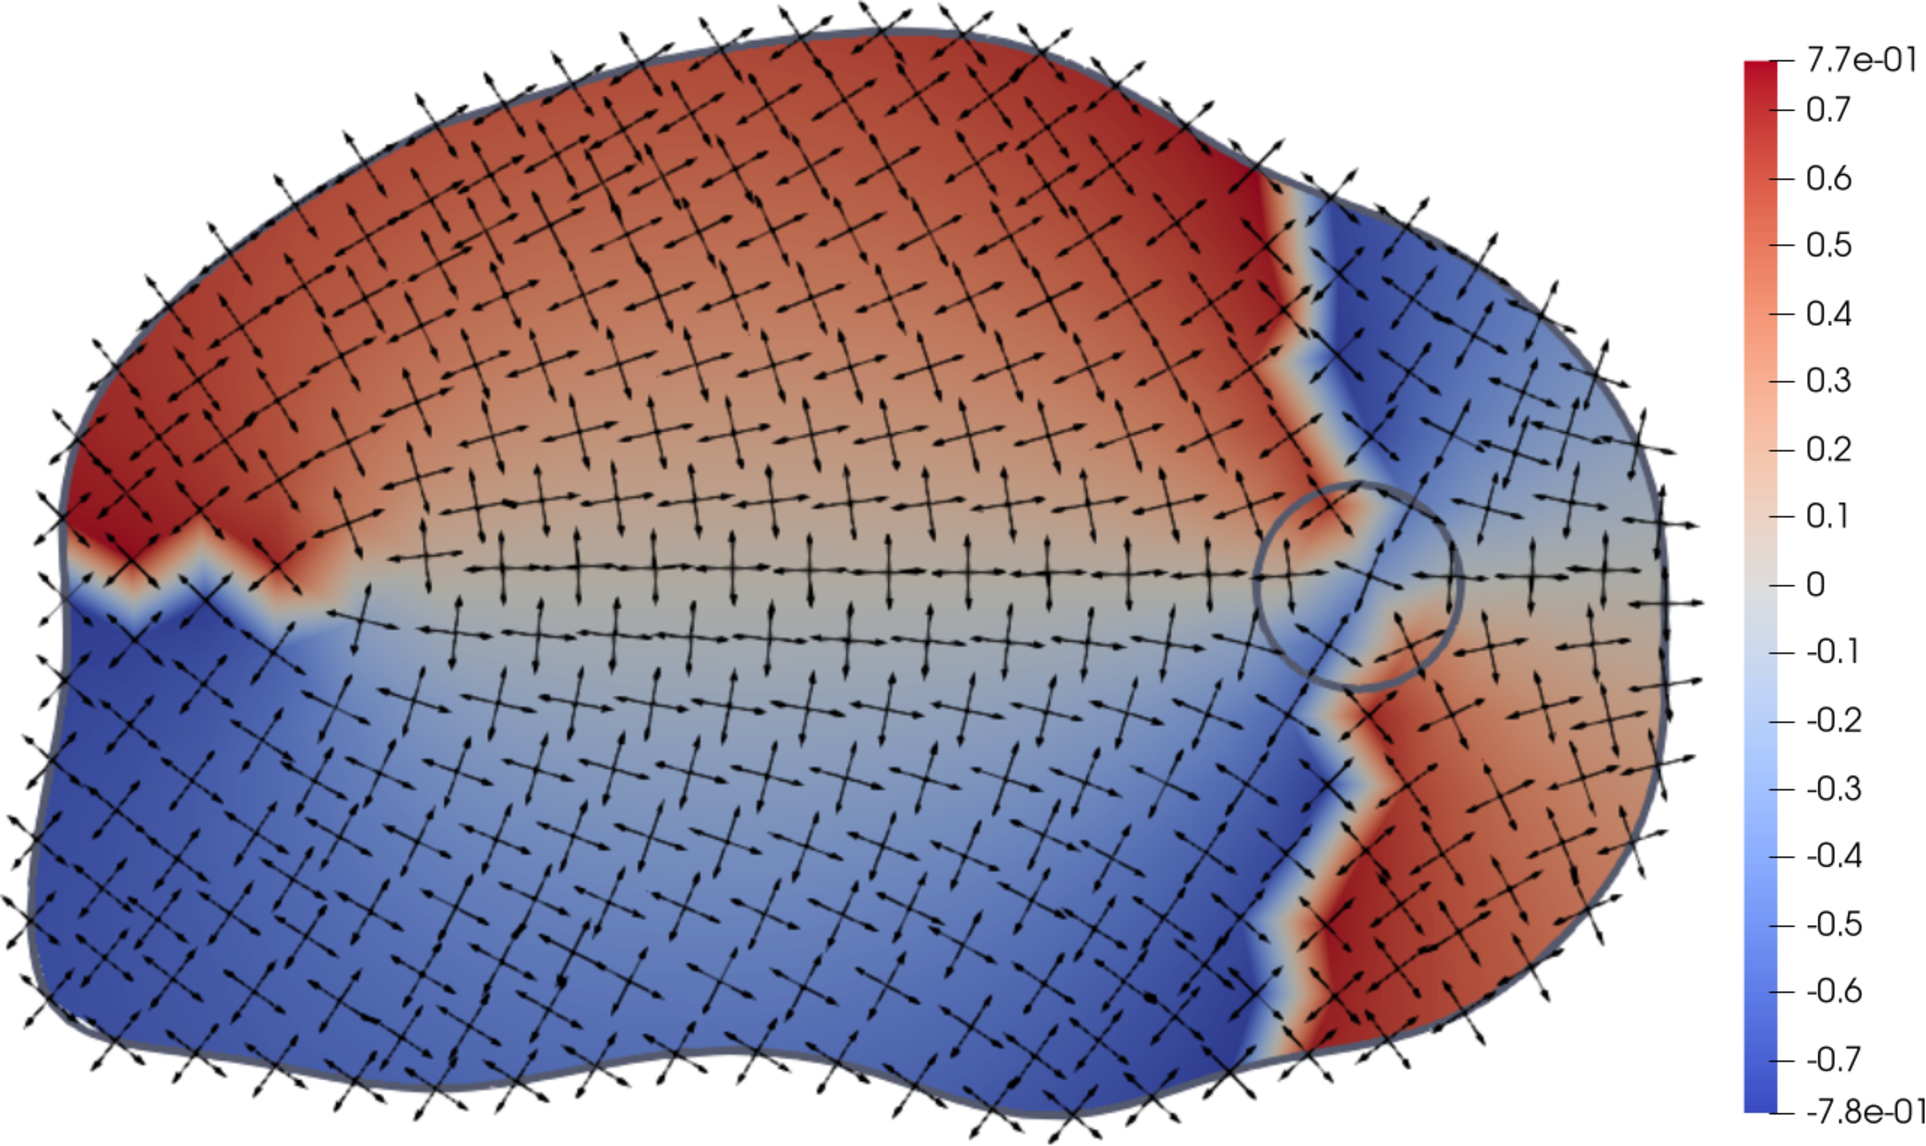
\includegraphics[scale=0.25]{images/lifting_cross_ang.pdf}\hspace{0.5cm}
  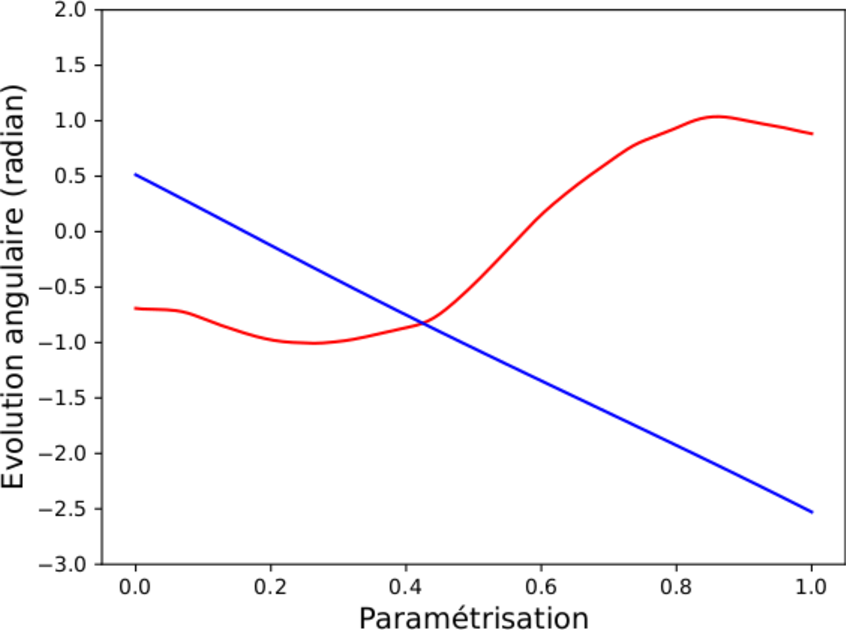
\includegraphics[scale=0.45]{images/lifting_courbe.pdf}
  \caption{Illustration du relèvement continu d'un champ de croix (à gauche avec son champ d'angle associé en radian) le long de courbes paramétriques. En bleu: la courbe paramétrique intérieur, en rouge la courbe paramétrique représentant le bord du domaine.}
  \label{fig:lifting}
\end{figure}
\end{comment}

\begin{definition}
    On appelle chemin fermé tout lacet $\Gamma$ qui soit $\mathcal{C}^0\cap\mathcal{C}^1_m$. On appellera paramétrisation simple de $\Gamma$, toute paramétrisation $\gamma : I\subset\mathbb{R}\longrightarrow\Gamma$ telle que l’ensemble $\{s\in I, \exists t\in I,~s\neq t,~ \gamma(s) = \gamma(t)\}$ est d’intérieur vide dans $\mathbb{R}$.
\end{definition}

Dans tout ce qui suit, les paramétrisations des lacets seront supposées être des paramétrisations simple et on aura par définition
$$
\int_\gamma f:=\int_If(\gamma(s)\gamma'(s)ds,
$$
indépendante de $\gamma$. On notera $V^\Gamma$ la partie de $\Omega$ délimitée par $\Gamma$. Soit $\overrightarrow{n}(q)$ la normale extérieur en $q$ à $\Gamma$. On dit que $\gamma$ paramétrise $\Gamma$ dans le sens positif si pour tout $t\in I$, $(\gamma'(t)\wedge\overrightarrow{n}(\gamma(t))).(0,0,1)^t>0$ Dans la suite, nous adoptons la notation suivante:

$$
\int_\Gamma d\theta_{\bar{u}}:=\int_\gamma d\theta_{\bar{u}}:=\int_a^b d\theta_{\bar{u}}^\gamma.
$$

\begin{lemma}
    \label{lem:index_saga_first}
    Soit $\bar{u}$ un champ de croix presque-$\mathcal{C}^1$ et $\Gamma$ un chemin fermé dont $\gamma$ est une paramétrisation sur $[a,b]$. La fonction $F(\Gamma)$ suivante
    $$
    F_{\bar{u}}(\Gamma):=\frac{1}{2\pi}\int_a^b d\theta_{\bar{u}}^\gamma,
    $$
    vérifie $4F_{\bar{u}}(\Gamma)\in\mathbb{Z}$. En outre, si $(V^{\Gamma_i})_{i\in\llbracket 1, n_\Gamma\rrbracket}$ forme une partition de $V^\Gamma$ tels que $\bar{u}(p)\neq 0,~\forall p\in\Gamma_i,~\forall i\in\llbracket 1, n_\Gamma\rrbracket$, alors on a:
    \begin{equation}
        F_{\bar{u}}(\Gamma)=\sum_{i=1}^{n_\Gamma}F_{\bar{u}}(\Gamma_i).
        \label{eqn:sum_F_u}
    \end{equation}
\end{lemma}

\begin{proof}
    Soit $w-z=e^{4i\theta_{\bar{u}}^\gamma}$ avec $z\in\mathbb{Z}$ alors
    $$
    2\pi F_{\bar{u}}(\Gamma)=\frac{1}{4}Im\left(\int_\gamma\frac{dw}{w-z}\right).
    $$
    Montrer que $4F_{\bar{u}}(\Gamma)\in\mathbb{Z}$ revient alors à montrer que:
    $$
    exp\left(\int_a^b\frac{w'(\gamma(t))\gamma'(t)}{w(\gamma(t))-z}dt\right)=1
    $$
    Posons
    $$
    \varphi(t):=exp\left(\int_a^t\frac{w'(\gamma(t))\gamma'(t)}{w(\gamma(t))-z}dt\right),~t\in[a,b],
    $$
    $\varphi$ est de classe $\mathcal{C}^1$ par morceau et vérifie:
    $$
    \frac{\varphi'}{\varphi}=\frac{\gamma'.w'\circ\gamma}{w'\circ\gamma-z},
    $$
    Il vient alors que la fonction $\varphi/(w\circ\gamma-z)$ est continue, dérivable presque partout ($w\in\mathcal{C}^1$ et $\gamma\in\mathcal{C}^0\cap\mathcal{C}^1_m$) de dérivée nulle donc elle est constante (presque partout, donc partout car continue) et comme $\varphi(a)=1$, on a:
    $$
    \varphi(t)=\frac{w(\gamma(t))-z}{w(\gamma(a))-z},
    $$
    En utilisant maintenant le fait que $\gamma(a)=\gamma(b)$, il vient que $\varphi(b)=1$ et donc finalement
    $$
    \exists k\in\mathbb{Z},~\int_a^b\frac{w'(\gamma(t))\gamma't)}{w(\gamma(t))-z}dt=2ik\pi.
    $$
    Ainsi $4F_{\bar{u}}(\Gamma)\in\mathbb{Z}$.\\\\
    Pour la propriété d'additivité de $F_{\bar{u}}$ on commence par décomposer les frontières de chaque $V^{\Gamma_i}$ de la manière suivante: $\Gamma_{i,0}=\Gamma_i\cap\Gamma$ et $\Gamma_{i,j}=\Gamma_i\cap\Gamma_j$ pour $j\neq i$. Par convention on pose $\Gamma_{i,i}=\emptyset$, $\forall i\in\llbracket 1, n_\Gamma\rrbracket$. On a alors $\Gamma_i=\cup_{i\in\llbracket1, n_\Gamma\rrbracket}\Gamma_{i,j}$ et $\Gamma_{i,j}=\Gamma_{j,i}$ et on peut écrire:
    $$
    \sum_{i=1}^{n_\Gamma}F_{\bar{u}}(\Gamma_i)=\frac{1}{2\pi}\sum_{i=1}^{n_\Gamma}\sum_{j=0}^{n_\Gamma}\int_{\Gamma_{i,j}}d\theta_{\bar{u}}^\gamma=\frac{1}{2\pi}\sum_{i=1}^{n_\Gamma}\int_{\Gamma\cap\Gamma_i}d\theta_{\bar{u}}+\frac{1}{2\pi}\sum_{i=1}^{n_\Gamma}\sum_{j=1}^{n_\Gamma}\int_{\Gamma_{i,j}}d\theta_{\bar{u}}.
    $$
    Autrement dit,
    $$
    \sum_{i=1}^{n_\Gamma}F_{\bar{u}}(\Gamma_i)=F_{\bar{u}}(\Gamma)+\frac{1}{2\pi}\sum_{i=1}^{n_\Gamma}\int_{\Gamma_{i,i}}d\theta_{\bar{u}}+\frac{1}{2\pi}\sum_{1\leq i<j\leq n_\Gamma}\int_{\Gamma_{i,j}\cup\Gamma_{j,i}}d\theta_{\bar{u}}.
    $$
    Dans l'équation précédente, le second terme s'annule car $\Gamma_{i,i}=\emptyset$ et le dernier terme vaut lui aussi zéro car $\Gamma_{i,j}\cup\Gamma_{j,i}$ représente un lacet et par hypothèse $\bar{u}$ est $\mathcal{C}^1$ sur $\Gamma_i\cap\Gamma_j$. D'où le résultat.
\end{proof}

\begin{lemma}
    \label{lem:index_saga_second}
    Sous les hypothèses du lemme \ref{lem:index_saga_first}, si $\bar{u}$ est $\mathcal{C}^1$ sur un ensemble convexe $V\subset\Omega$ alors pour tout arc $\Gamma$ de longueur assez petite telle que $V^\Gamma\subset V$ on a $F_{\bar{u}}(\Gamma)=0$.
\end{lemma}

\begin{proof}
    Il suffit de remarquer que si $u$ est de classe $\mathcal{C}^1$ sur $V^\Gamma$ alors $w'$ est bornée par une constante $M>0$ sur $V^\Gamma$ et donc on a:
    $$
    \left|\int_a^b\frac{w'(\gamma(t))\gamma't)}{u(\gamma(t))-z}dt\right|\leq M\int_a^b|\gamma'(t)|dt<2\pi,
    $$
    pour $\Gamma$ décrivant un arc de longueur inférieure à $2\pi/M$, tel que $V^\Gamma\subset V$ et donc $F_u(\Gamma)=0$.
\end{proof}

\begin{lemma}
    \label{lem:index_saga_third}
    Pour tout voisinnage $V^\Gamma$ de $p$ tel que $u\in\mathcal{C}^1(V^\Gamma\backslash\{p\})$, on a pour tous chemins fermés $\Gamma_1$ et $\Gamma_2$ on a:
    $$
    p\in V^{\Gamma_i}\subset V^\Gamma, \forall i=1, 2\Longrightarrow F_{\bar{u}}(\Gamma_1)=F_{\bar{u}}(\Gamma_2).
    $$
\end{lemma}

\begin{proof}
    Soient $\Gamma_1$et $\Gamma_2$ deux lacets vérifiant les hypothèses du lemme. En notant $V_3=V^{\Gamma_1}\cap V^{\Gamma_2}$ et $\Gamma_3=\partial V^{\Gamma_3}$ qui est $\mathcal{C}^0\cap\mathcal{C}^1_m$ et $(V^i_j)_{j\in\llbracket 1, k_i\rrbracket}$ les composantes connexes de $v^{\Gamma_i}\backslash V^3$, pour $i=1,2$. En notant $\Gamma_i^j=\partial V^i_j$, qui est donc $\mathcal{C}^0\cap\mathcal{C}^1_m$. En appliquant \eqref{eqn:sum_F_u},on obtient:
    $$
    \forall i=1,2,~F_{\bar{u}}(\Gamma_i)=\sum_{j=1,\dots,k_i}F_{\bar{u}}(\Gamma_i^j)=F_{\bar{u}}(\Gamma_3),
    $$
    par le lemme \ref{lem:index_saga_second} car $u$ est $\mathcal{C}^1$ sur chaque $V^i_j\subset V^\Gamma\backslash\{p\}$. D'où le résultat.
\end{proof}

En combinant les lemmes \ref{lem:index_saga_first} et \ref{lem:index_saga_second}, on obtient alors:

\begin{definition}
    Pour un champ $u$ n'ayant que des irrégularités isolées, on appelle indice du point p dans le champ $u$ la valeur:
    $$
    id_{\bar{u}}(p):=F_{\bar{u}}(\Gamma),
    $$
    où $\Gamma$ est un chemin fermé paramétré dans le sens positif tel que $p\in V^\Gamma$ et $u\in\mathcal{C}^1(V^\Gamma\backslash\{p\})$.
    \label{def:index}
\end{definition}

\begin{proposition}
    La définition \ref{def:index} est bien posée.
\end{proposition}

\begin{proof}
    Il s'agit d'une conséquence directe du lemme \ref{lem:index_saga_third}.
\end{proof}

On peut alors retrouver les propriétés principales de l'indice, résumées dans le théorème suivant:

\begin{theorem}
    L'indice du point $p$ dans le champ $u$ vérifie les propriétés suivantes:
    \begin{enumerate}
        \item $id_{\bar{u}}^\gamma(p)\in\mathbb{Z}$,
        \item si $u$ est $\mathcal{C}^1$ en $p$ alors $ind_u(p)=0$,
        \item pour tout chemin fermé $\Gamma$ tel que $p\in V^\Gamma$ et que $u\in\mathcal{C}^1(V^\Gamma\backslash\{p\})$, $id_{\bar{u}}^\gamma(p)=F_{\bar{u}}(\Gamma)$.
    \end{enumerate}
\end{theorem}

\begin{proof}
    Ces résultats sont respectivement des conséquences directes des lemmes \ref{lem:index_saga_first}, \ref{lem:index_saga_second} et \ref{lem:index_saga_third}.
\end{proof}

\begin{comment}
    \begin{definition}[Indice]
    \label{def:index}
    Soit $\bar{u}$ un champ de croix presque-$\mathcal{C}^1$ définit sur $\Omega$ et un point $p$ dans $\Omega\backslash\partial\Omega$. L'indice de $p$ dans le champ de croix $\bar{u}$ est donné par la quantité:
    \begin{equation}
    id_{\bar{u}}(p) =\frac{1}{2\pi}\int_0^1d\theta_{\bar{u}}^\gamma,
    \label{eqn:Indexinterior}
    \end{equation}
    où $\gamma :[0 ; 1]\longrightarrow \Omega$ est un lacet entourant $p$, n'englobant aucun autre point singulier de $\bar{u}$ et paramétrisé dans le sens anti-horaire.
    \end{definition}
\end{comment}

De manière intuitive, l'indice d'un point dans un champ exprime combien de fois le champ semble s'enrouler autour de lui-même près de ce point (voir la figure \ref{fig:index_illustration}).

\begin{figure}[!h]
  \centering
  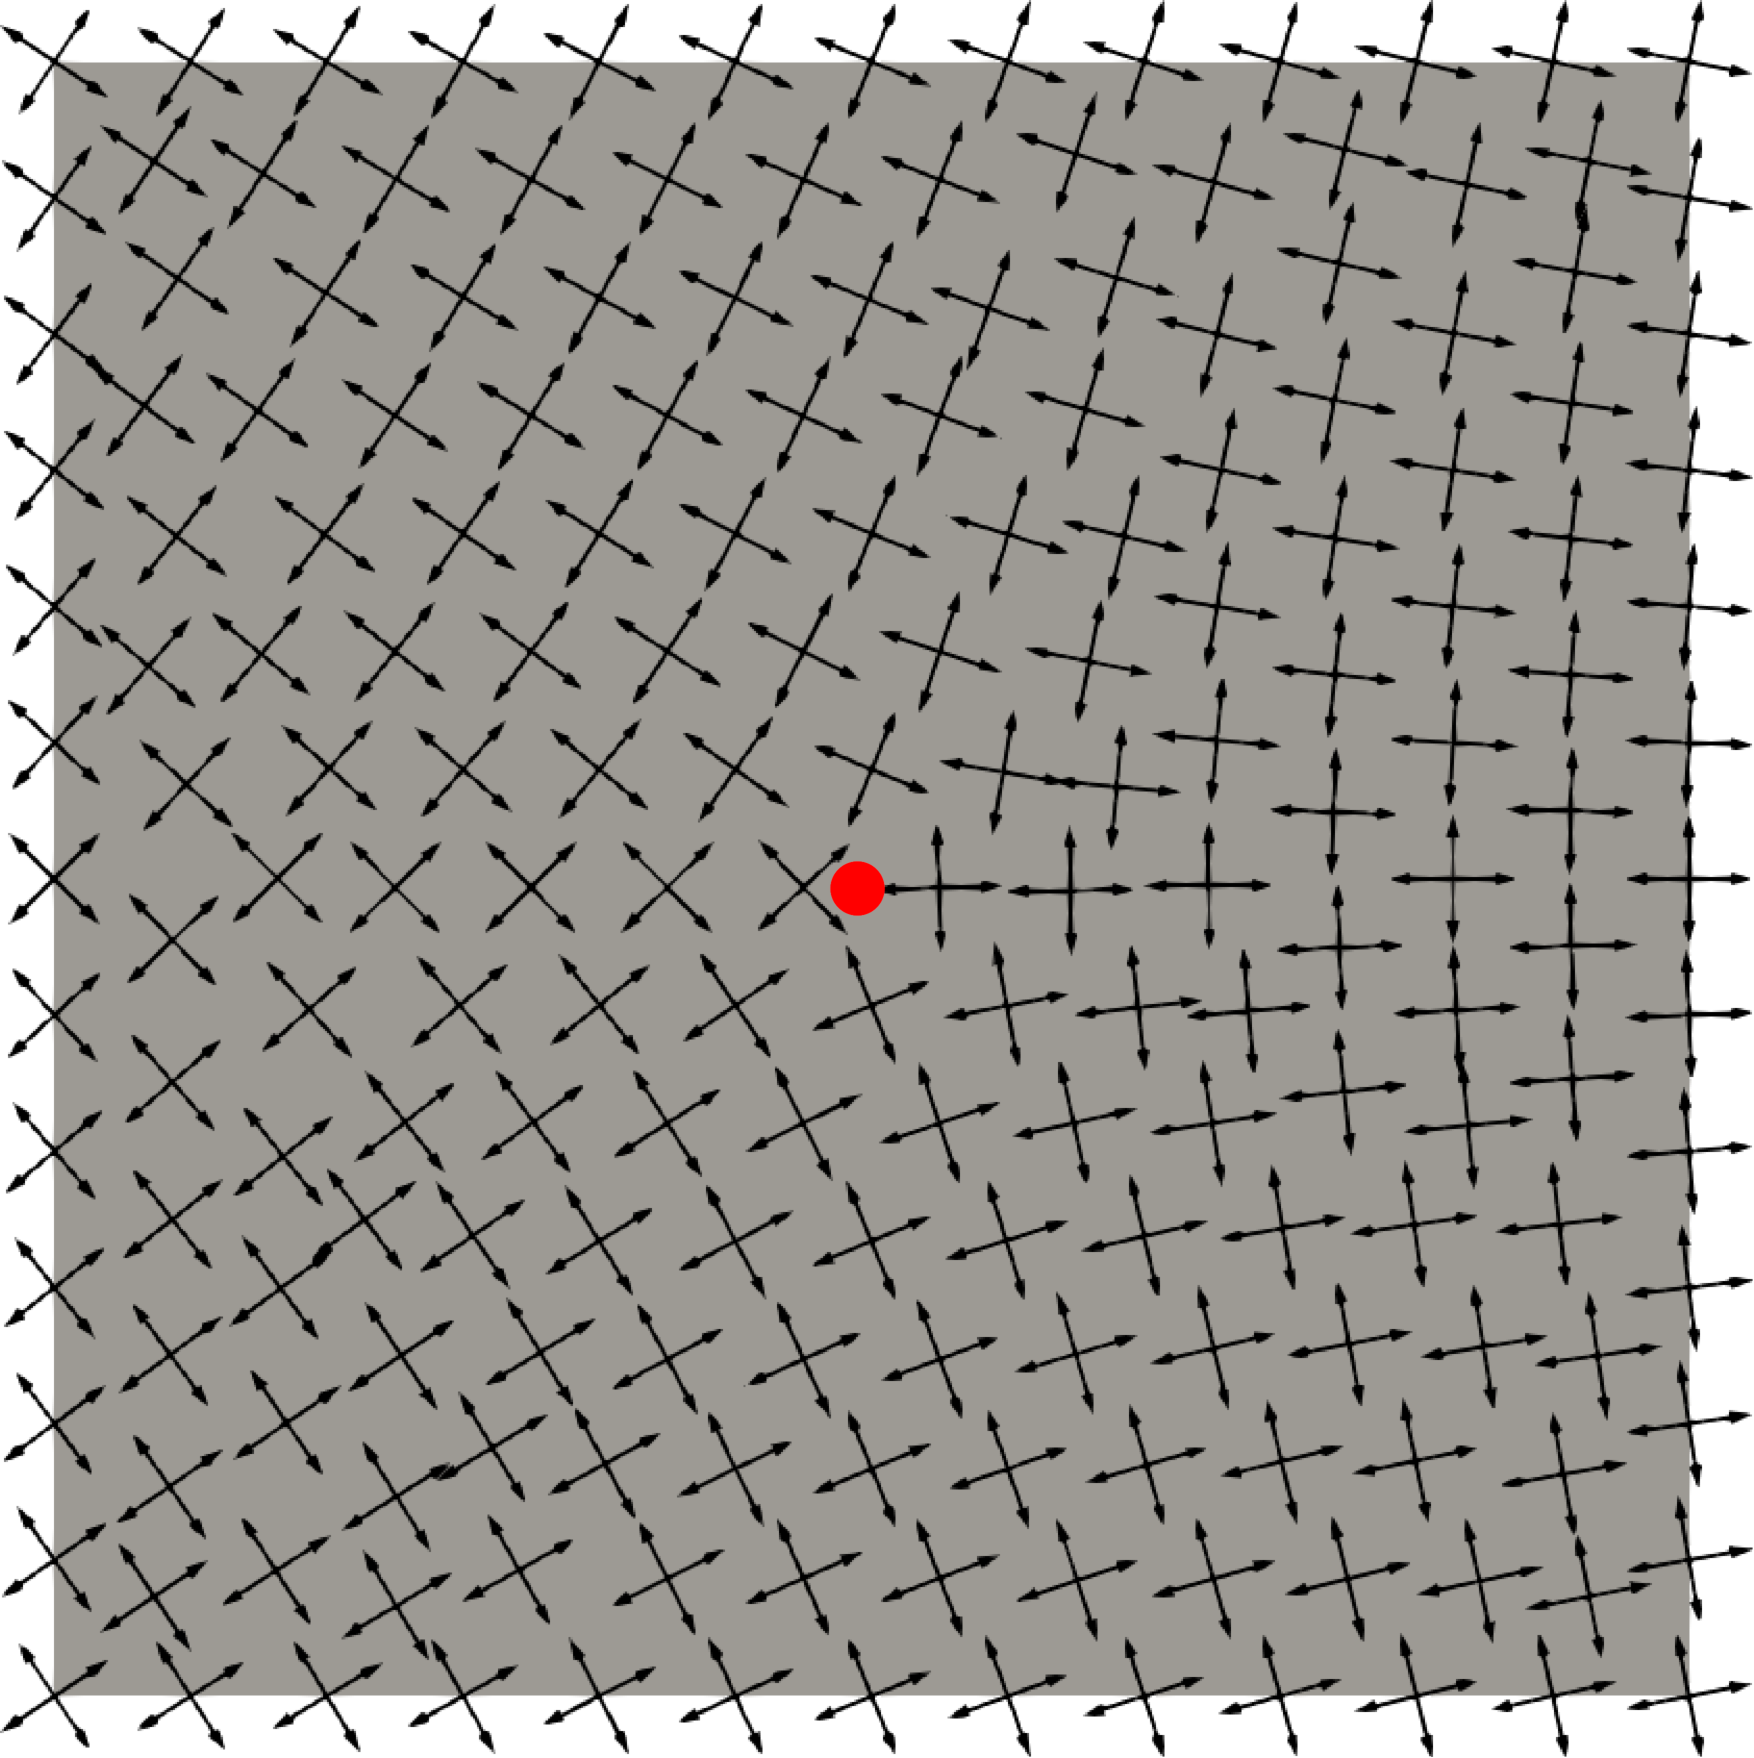
\includegraphics[scale=0.25]{images/index_-025.pdf}
  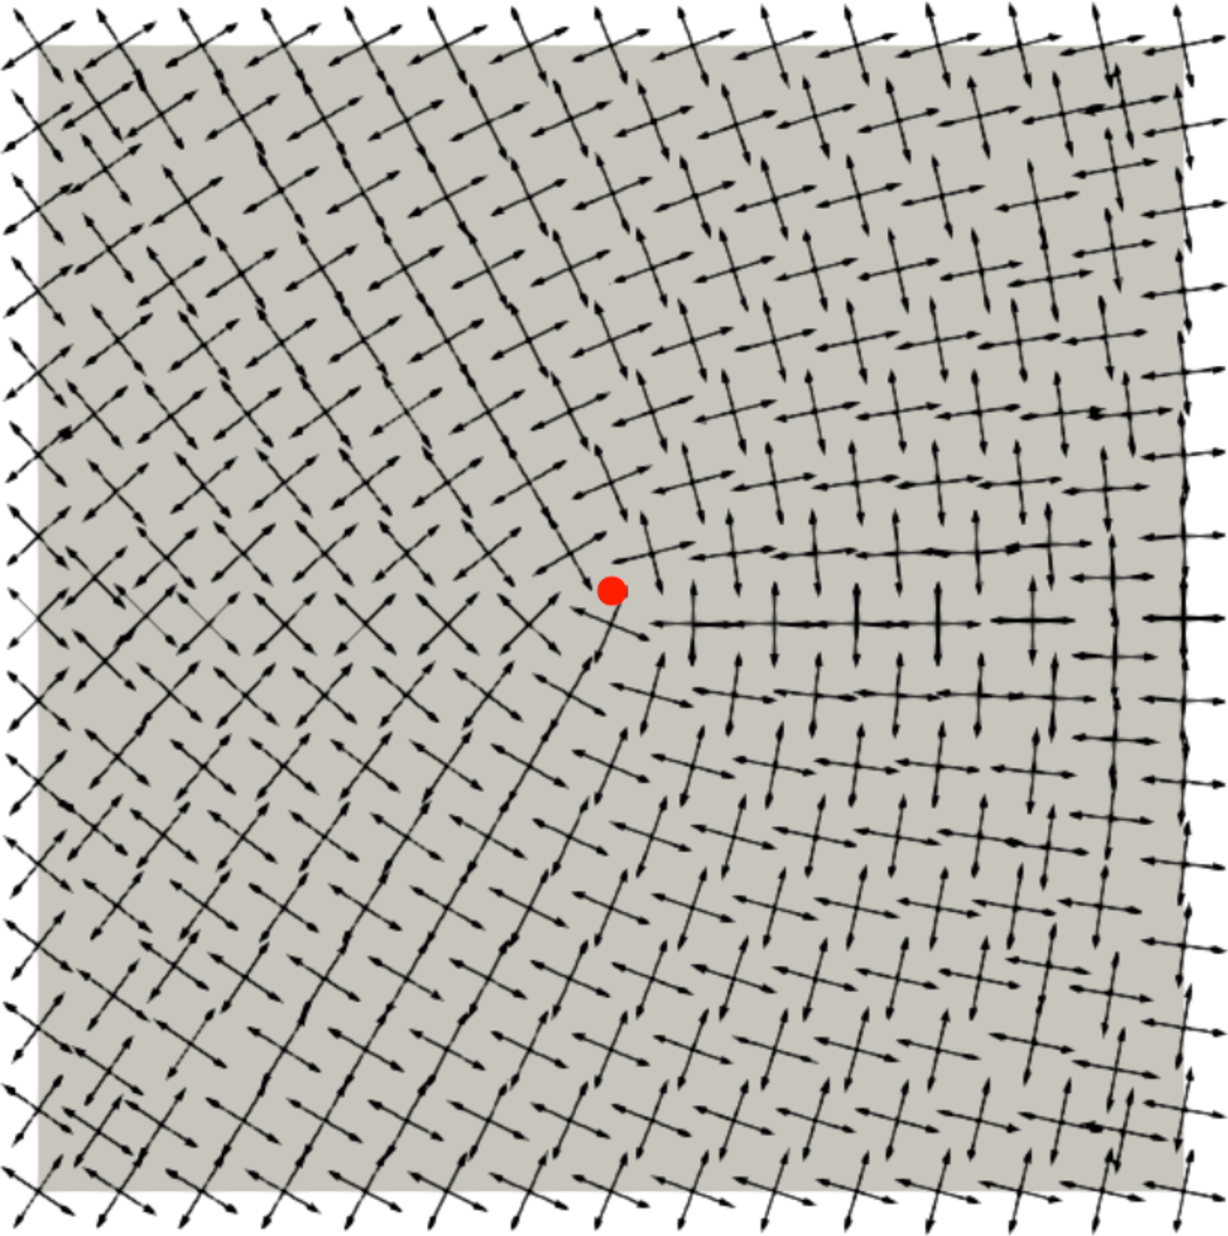
\includegraphics[scale=0.25]{images/index_025.pdf}
  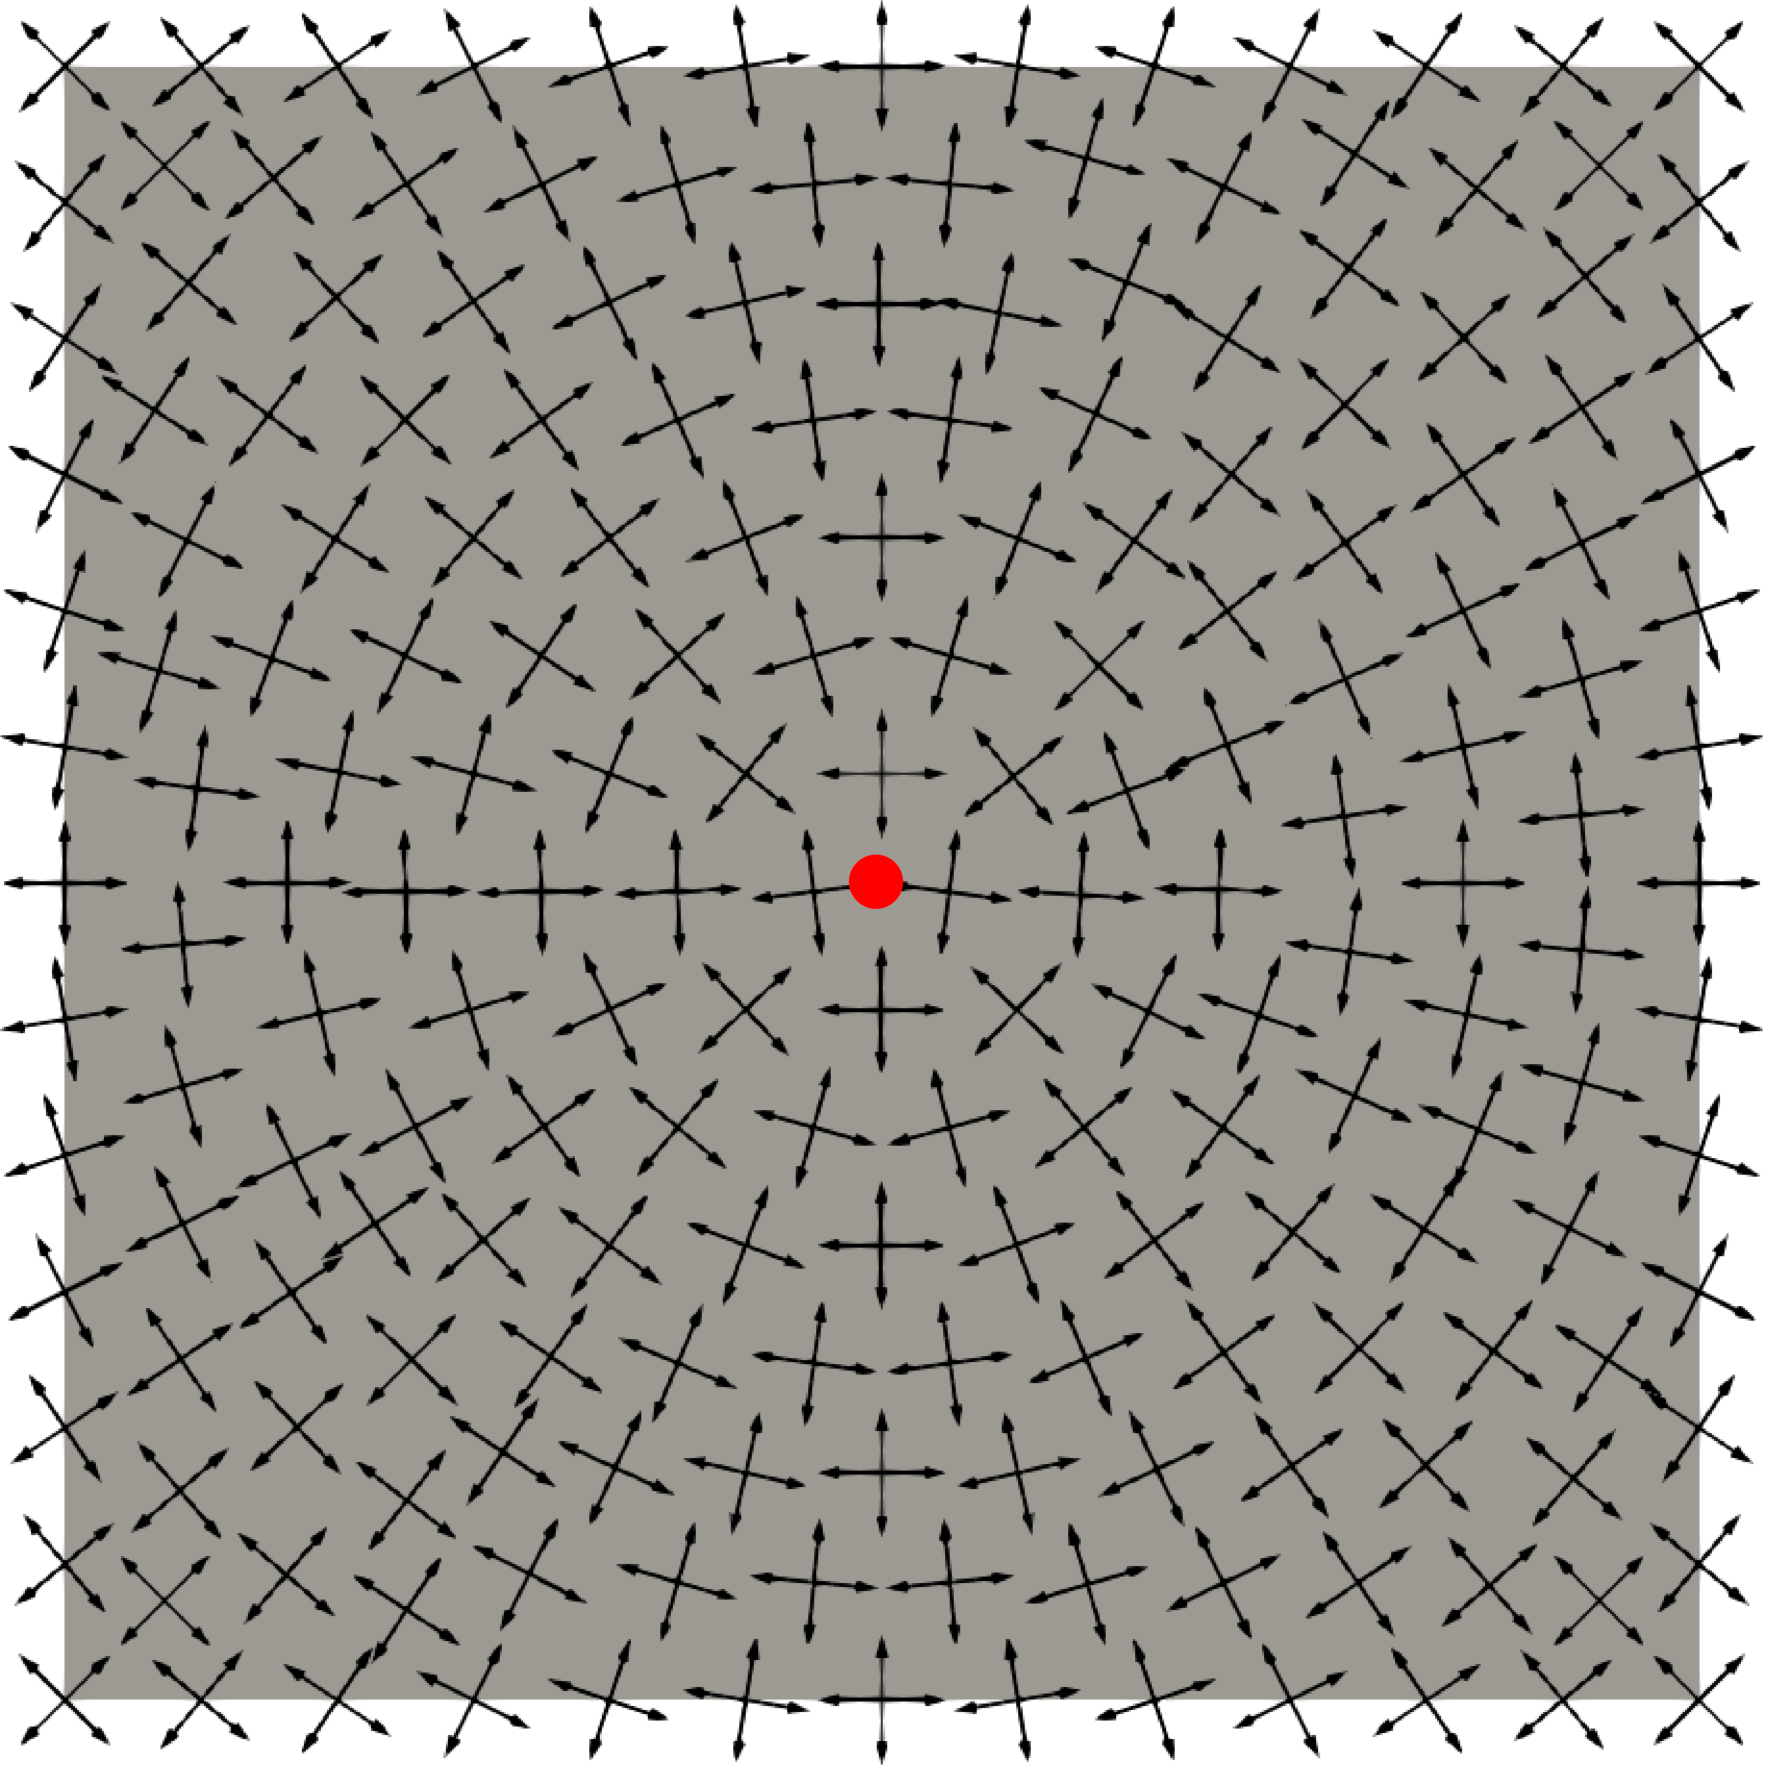
\includegraphics[scale=0.25]{images/index_1.pdf}
  \caption{Gauche: $id_{\bar{u}}(p)=-\frac{1}{4}$, milieu: $id_{\bar{u}}(p)=\frac{1}{4}$, droite: $id_{\bar{u}}(p)=1$}
  \label{fig:index_illustration}
\end{figure}

Après avoir énoncé cette définition, on peut se demander comment l'indice d'un point évolue lorsqu'on effectue rotation sur le champ de croix. Le résultat suivant fournit une réponse à cette interrogation.

\begin{proposition}
\label{prop:relation_u_Rthetau}
Soit $\bar{u}$ un champ de croix presque-$\mathcal{C}^1$ sur $\Omega$ et $\theta:\Omega \rightarrow \mathbb{R}$ une fonction de classe $\mathcal{C}^1$ sur $\Omega$, alors pour tout $p\in \Omega\backslash\partial\Omega,~id_{\bar{u}}(p)=id_{\mathbf{R}(\theta)\bar{u}}(p)$.
\end{proposition}

\begin{proof}
Posons $\bar{v}:=\mathbf{R}(\theta)\bar{u}$. Soit $p\in\Omega\backslash\partial\Omega$ et $\gamma:[0, 1]\longrightarrow\Omega$ un lacet dans $\Omega$ entourant $p$ et n'englobant aucun autre point singulier de $\bar{u}$. $\bar{u}$ étant un champ de croix presque-$\mathcal{C}^1$ sur $\Omega$, il existe donc $\theta_{\bar{u}}^\gamma\in\mathcal{C}^1(]0, 1[)$. Soit $\theta_{\bar{v}}^\gamma:=\theta\circ\gamma+\theta_{\bar{u}}^\gamma$. D'une part $\theta_{\bar{v}}^\gamma$ est de classe $\mathcal{C}^1$ sur $]0, 1[$ puisque $\theta\in\mathcal{C}^1(\Omega)$. D'autre part d'après la proposition \ref{prop:angular_cont}, $\theta_{\bar{v}}^\gamma(t)\equiv\theta(\gamma(t))+\theta_{\bar{u}}(\gamma(t))\pmod{\frac{\pi}{2}}$ et en utilisant la proposition \ref{prop:cont1} il vient que $\theta_{\bar{v}}^\gamma(t)\equiv\theta_{\bar{v}}(\gamma(t))\pmod{\frac{\pi}{2}}$. On a donc:
\begin{eqnarray*}
    id_{\bar{v}}(p)&=&\frac{1}{2\pi}\int_0^1 d\theta_{\bar{v}}^\gamma,\\
    &=&\frac{1}{2\pi}\left[\int_0^1 d(\theta\circ\gamma)+\int_0^1 d\theta_{\bar{u}}^\gamma\right],\\
    id_{\bar{v}}(p)&=&\frac{1}{2\pi}\left[\oint_\gamma d\theta+\int_0^1 d\theta_{\bar{u}}^\gamma\right].
\end{eqnarray*}
Or $\oint_\gamma d\theta=0$ puisque $\theta\in\mathcal{C}^1(\Omega)$. Autrement dit on a:
$$id_{\bar{v}}(p)=\frac{1}{2\pi}\int_0^1 d\theta_{\bar{u}}^\gamma=id_{\bar{u}}(p).$$
\end{proof}

Si $p\in\partial\Omega$ et le champ de croix $\bar{u}$ est aligné avec $\partial\Omega$, nous construisons une extension à la définition \ref{def:index} de la manière suivante: nous choisissons un lacet $\gamma\subset\Omega$ et paramétré sur $[0, 1]$ tel que $\gamma(0)=p=\gamma(1)$ et les vecteurs $\gamma'(0)$ et $\gamma'(1)$ sont tangents à $\partial\Omega$. On suppose de plus que $\gamma$ n'englobe pas d'autres points singulier de $\bar{u}$ à par $p$. L'indice de $p$ est alors donné par:

\begin{equation}
id^\partial_{\bar{u}}(p) = \frac{1}{2\pi}\left[\pi-\hat{p}+\underbrace{\lim\limits_{s\rightarrow 0}\int_s^{1-s}d\theta_{\bar{u}}^\gamma}_{\delta\theta(p)}\right]=\frac{1}{2\pi}\left[\pi-\hat{p}+\delta\theta(p)\right],
\label{eqn:Indexboundary}
\end{equation}
où $\hat{p}$ est la mesure de l'angle d'ouverture du bord en $p$. %Nous reviendrons sur cette définition dans la partie \ref{subsec:etude_de_la_methode} pour donner un lien entre l'index intérieur et l'index de bord.

\subsection{Théorème de Poincaré-Hopf}
\label{subsec:Poincare_Hopf}

Le théorème de Poincaré-Hopf constitue un résultat fondamental en topologie différentielle, établissant un lien profond entre les propriétés topologiques d'une variété différentielle compacte et les singularités d'un champ de vecteurs défini sur cette variété. Ce théorème fournit une manière précise de quantifier le nombre et le type de points singuliers d'un champ de vecteurs sur une variété compacte. En particulier, il établit une relation entre la somme des indices de ces points singuliers et la caractéristique d'Euler de la variété. Les auteurs de \cite{ray2008n} fournissent une adaptation de ce théorème aux champs de croix. Ainsi si $\bar{u}$ est un champ de croix presque-$\mathcal{C}^1$ sur $\Omega$ et aligné avec $\partial\Omega$ alors nous avons la formule suivante:

\begin{equation}
    \label{eqn:first_Poincare_Hopf}
    \sum_i id_{\bar{u}}(s_i)=\chi(\Omega),
\end{equation}
où la somme est celle des indices des points singuliers de $\bar{u}$ et $\chi(\Omega)$ est la caractéristique d'Euler de $\Omega$. Pour prendre en considération les champs de croix comportant des points singuliers situés sur la frontière du domaine, nous construisons un domaine $\Omega^\epsilon$ englobant $\Omega$ dont la frontiere est une isoline de valeur $\epsilon$ obtenu via la résolution de l'équation de la chaleur dans $\mathbb{R}^2\backslash\Omega$ et tel que $\partial\Omega^\epsilon\cap\Omega=\emptyset$. On construit ensuite le champ de croix $\bar{u}^\epsilon$ pour tout $p\in\Omega^\epsilon$ par:
$$
\bar{u}^\epsilon(p)=
\left\{
\begin{array}{ll}
\bar{u}(p)& \mbox{ si } p\in\Omega,\\[0.5cm]
\left\{\mathbf{R}\left(\displaystyle\frac{m\pi}{2}\right)f(p),~ m\in \mathbb{Z}\right\} & \mbox{ sinon },
\end{array}
\right.
$$
où pour tout $p\in\Omega^\epsilon\backslash\Omega$, $f$ désigne le vecteur gradient à l'isoline en $p$. Par construction, $\bar{u}^\epsilon$ est aligné sur le bord de $\Omega^\epsilon$ et $\mathcal{S}_{\bar{u}^\epsilon}\cap\partial\Omega^\epsilon=\emptyset$ Autrement dit, on a:
$$
\sum_{p\in\mathcal{S}_{\bar{u}^\epsilon}} id_{\bar{u}^\epsilon}(p)=\chi(\Omega^\epsilon)
$$
Or $\chi(\Omega^\epsilon)=\chi(\Omega)$ donc on a:
$$
\sum_{p\in\mathcal{S}_{\bar{u}^\epsilon}\backslash\partial\Omega} id_{\bar{u}^\epsilon}(p)+\sum_{p\in\mathcal{S}_{\bar{u}^\epsilon}\cap\partial\Omega} id_{\bar{u}^\epsilon}(p)=\chi(\Omega).
$$
Sachant que pour tout $p\in\partial\Omega$ on a $id_{\bar{u}^\epsilon}(p)=id^\partial_{\bar{u}}(p)$ alors
\begin{eqnarray}
    \label{eqn:poin_hopf_gen}
    \sum_{p\in\mathcal{S}_{\bar{u}}\backslash\partial\Omega} id_{\bar{u}}(p)+\sum_{p\in\mathcal{S}_{\bar{u}}\cap\partial\Omega} id^\partial_{\bar{u}}(p)&=&\chi(\Omega).
\end{eqnarray}
Nous posons alors l'équation \eqref{eqn:poin_hopf_gen} comme la généralisation de la formule de Poincaré-Hopf aux champs de croix aligné sur le bord du domaine et possédant des points singuliers de bord.


\begin{comment}
Pour prendre en considération les champs de croix comportant des points singuliers situés sur la frontière du domaine, nous introduisons le lemme suivant. Celui-ci établit une relation entre l'indice d'un point sur la frontière dans un champ de croix et l'indice intérieur de ce point dans un champ de croix étendu sur une zone englobant le point.
 \begin{lemma}
    \label{lem:lemme_poinc_hopf}
    Soit $\bar{u}$ un champ de croix presque-$\mathcal{C}^1$ sur $\Omega$ et aligné avec le bord de $\Omega$ et soit $p\in\partial\Omega$. Il existe un voisinnage $V_p\subset\mathbb{R}^2$ de $p$ et un champ de croix $\bar{v}$ presque-$\mathcal{C}^1$ sur $\Omega\cup V_p$ tel que $\mathcal{S}_{\bar{v}}=\mathcal{S}_{\bar{u}}$ et $id_{\bar{v}}(p) = id^\partial_{\bar{u}}(p)$.
\end{lemma}

\color{red}
\begin{proof}
    Soit $V_p=\bar{\mathcal{D}(p, \epsilon)}\backslash\mathring{\Omega}$ où $\bar{\mathcal{D}(p, \epsilon)}$ est le disque fermé centré en $p$ et de rayon $\epsilon>0$, tel que $\bar{\mathcal{D}(p, \epsilon)}\cap\partial\Omega=[pa]\cup[pb]$ avec $\{a, b\} = \partial\bar{\mathcal{D}(p, \epsilon)}\cap\partial\Omega$. $[pa]$ (respectivement $[pb]$) désigne le segment de droite $(pa)$ (respectivement $(pb)$) et les points $a$ et $b$ sont choisis de tel sorte que $\overrightarrow{ap}\wedge\overrightarrow{pb}>0$. On suppose de plus que $(V_p\cap\mathcal{S}_{\bar{u}})\backslash\{p\}=\emptyset$. Remarquons que $\Omega\cap V_p=[pa]\cap[pb]$. Soit $f$ la fonction définie pour tout $q\in V_p$ par:

    \begin{equation}
    f(q)=
    \left\{
    \begin{array}{ll}
        N(q) & \mbox{ si } q\in[pa],\\[0.5cm]
        \mathbf{R}\left(\alpha(\tau(q))\left(1-\displaystyle\frac{\pi}{2\pi-\hat{p}}\right)\right)N(\tau(q)) & \mbox{ sinon },
    \end{array}
    \right.
    \end{equation}
    où $\tau(q)=p+\|\overrightarrow{pq}\|.\|\overrightarrow{pa}\|^{-1}\overrightarrow{pa}$ et $\alpha(\tau(q))=\widehat{\tau(q)pq}$ est l'angle orienté entre les vecteurs $\overrightarrow{p\tau(q)}$ et $\overrightarrow{pq}$. Il est clair que $f$ est de classe $\mathcal{C}^1$ dans $V_p\backslash\{p\}$ puisque $\tau,\alpha\in\mathcal{C}^1(V_p\backslash\{p\}))$ et que la normale $N$ est $\mathcal{C}^1$ sur $]pa]$. Par conséquent, d'après la Propostion \ref{prop:cont1} le champ de croix $\bar{w}$ défini pour tout $q\in V_p$ par:
    \begin{equation}
    \bar{w}(q)=
    \left\{
    \begin{array}{ll}
        \bar{N}(p) & \mbox{ si } q=p,\\[0.5cm]
        \left\{\mathbf{R}\left(\displaystyle\frac{m\pi}{2}\right)f(q),~ m\in \mathbb{Z}\right\} & \mbox{ sinon },
    \end{array}
    \right.
    \end{equation}
    est presque-$\mathcal{C}^1$ sur $V_p\backslash\Omega$. Remarquons que pour tout $q\in\Omega\cap V_p$, $\bar{u}(q)=\bar{w}(q)$ puisque par définition si $q\in[pa]$, $\bar{u}(q)=\bar{w}(q)$ et pour tout $q\in]pb]$, $f(q)$maintenant $\bar{v}$, le champ de croix défini pour tout $q\in\Omega\cup V_p$ par:
    \begin{equation}
    \bar{v}(q)=
    \left\{
    \begin{array}{lcll}
    \bar{u}(q) & \mbox{ si } q\in\Omega,\\[0.5cm]
    \bar{w}(q) & \mbox{ sinon }.
    \end{array}
    \right.
    \end{equation}
    $\bar{v}$ est presque-$\mathcal{C}^1$ sur $\Omega\cup V_p$ avec $\mathcal{S}_{\bar{v}}=\mathcal{S}_{\bar{u}}$ et $id_{\bar{v}}(p)=id_{\bar{u}}(p)$. On a alors:
    \begin{eqnarray*}
        id_{\bar{w}}(p)&=&\int_{\partial V_p}d\theta_{\bar{w}},\\
        &=&\int_{\partial V_p\backslash\Omega}d\theta_{\bar{w}}+\int_{\partial V_p\backslash(\partial V_p\backslash\Omega)d\theta_{\bar{w}}}d\theta_{\bar{w}}\\\\
        id_{\bar{w}}(p)&=&\pi-\hat{p}+2\pi id^\partial_{\bar{u}}(p)-\pi+\hat{p}.
    \end{eqnarray*}
Ce qui montre que $id_{\bar{w}}(p)=id^\partial_{\bar{u}}(p)$.
\end{proof}
\color{black}
Grâce à ce lemme, la formule de Poincaré-Hopf \eqref{eqn:first_Poincare_Hopf} peut être écrite sur le domaine $\Omega\cup(\cup_{p\in\mathcal{S}_{\bar{u}}\cap\partial\Omega}V_p)$. Autrement dit, on a:
$$
\sum_{p\in\mathcal{S}_{\bar{w}}} id_{\bar{w}}(p)=\chi(\Omega\cup(\cup_{p\in\mathcal{S}_{\bar{u}}\cap\partial\Omega}V_p))
$$
Or $\chi(\Omega\cup(\cup_{p\in\mathcal{S}_{\bar{u}}\cap\partial\Omega}V_p))=\chi(\Omega)$ donc on a:
$$
\sum_{p\in\mathcal{S}_{\bar{w}}\backslash\partial\Omega} id_{\bar{w}}(p)+\sum_{p\in\mathcal{S}_{\bar{w}}\cap\partial\Omega} id_{\bar{w}}(p)=\chi(\Omega).
$$
D'après le lemme \ref{lem:lemme_poinc_hopf} on a $id_{\bar{w}}(p)=id^\partial_{\bar{u}}(p)$ pour tout $p\in\mathcal{}$:
\begin{eqnarray}
    \label{eqn:poin_hopf_gen}
    \sum_{p\in\mathcal{S}_{\bar{u}}\backslash\partial\Omega} id_{\bar{u}}(p)+\sum_{p\in\mathcal{S}_{\bar{w}}\cap\partial\Omega} id^\partial_{\bar{u}}(p)&=&\chi(\Omega).
\end{eqnarray}
Nous posons alors l'équation \eqref{eqn:poin_hopf_gen} comme la généralisation de la formule de Poincaré-Hopf aux champs de croix aligné sur le bord du domaine et possédant des points singuliers de bord.
\end{comment}

\subsection{Ligne de champ et séparatrices}

Le dernier point de cette section concerne un outil indispensable dans la technique de maillage qui est la construction de lignes de champ. En réalité, ces lignes seront les frontières des sous-régions générées par l'algorithme.
Comme pour les champs vectoriels, une ligne de champ d'un champ de croix $\bar{u}$ est définie comme une courbe continûment différentiable dans $\Omega$. Plus précisément, nous avons la définition suivante :

\begin{definition}
\label{def:SL}
Soit $\bar{u}$ un champ croisé presque-$\mathcal{C}^1$. Étant donné un point $p_0\in \Omega\backslash \mathcal{S}_{\bar{u}}$ et une direction $\overrightarrow{u_0}\in \bar{u}(p_0)$, une ligne de champ émanant de $p_0$ selon $\overrightarrow{u_0}\in \mathbb{R}^2$, notée par $SL{\bar{u}}(p_0,\overrightarrow{u_0})$, est la courbe $S$ telle que :

\begin{enumerate}
\item il existe $\pi_{\bar{u}}^S:\Omega\longrightarrow\mathbb{R}^2$ une application telle que $\pi_{\bar{u}}^S(p_0)=\overrightarrow{u_0}$ et pour tout $p\in Im S$ il existe un voisinnage $V_p$ de $p$ tel que:
\begin{equation}
\label{eqn:pi_u_S}
\pi_{\bar{u}}^S\in\mathcal{C}^1(V_p) \mbox{ et }  \forall q\in V_p, \pi_{\bar{u}}^S(q)\in \bar{u}(q),
\end{equation}
\item $S$ est une solution maximale dans $\Omega$ de l'équation différentielle
\begin{equation}
\label{eqn:streamline}
\frac{dS(t)}{dt}=\pi_{\bar{u}}^S(S(t)),t\in \mathbb{R} \text{ et }  S(0)=p_0.
\end{equation}
\end{enumerate}
\end{definition}

\begin{lemma}
\label{lem:def_streamline_lemma}
La courbe $SL_{\bar{u}}(p_0,\overrightarrow{u_0})$ proposée dans la définition~\ref{def:SL} est bien définie.
\end{lemma}

\begin{proof}
Pour établir ce lemme, nous construisons d'abord l'application $\pi$ restreinte au voisinage de $p$ et procédons ensuite à la construction de la ligne de champ restreinte au voisinage de $p$. La ligne de champ complète est ensuite formée en étendant itérativement cette construction à chaque voisinage successif (voir figure \ref{fig:streamline_construction}).\
\begin{figure}[!h]
\centering
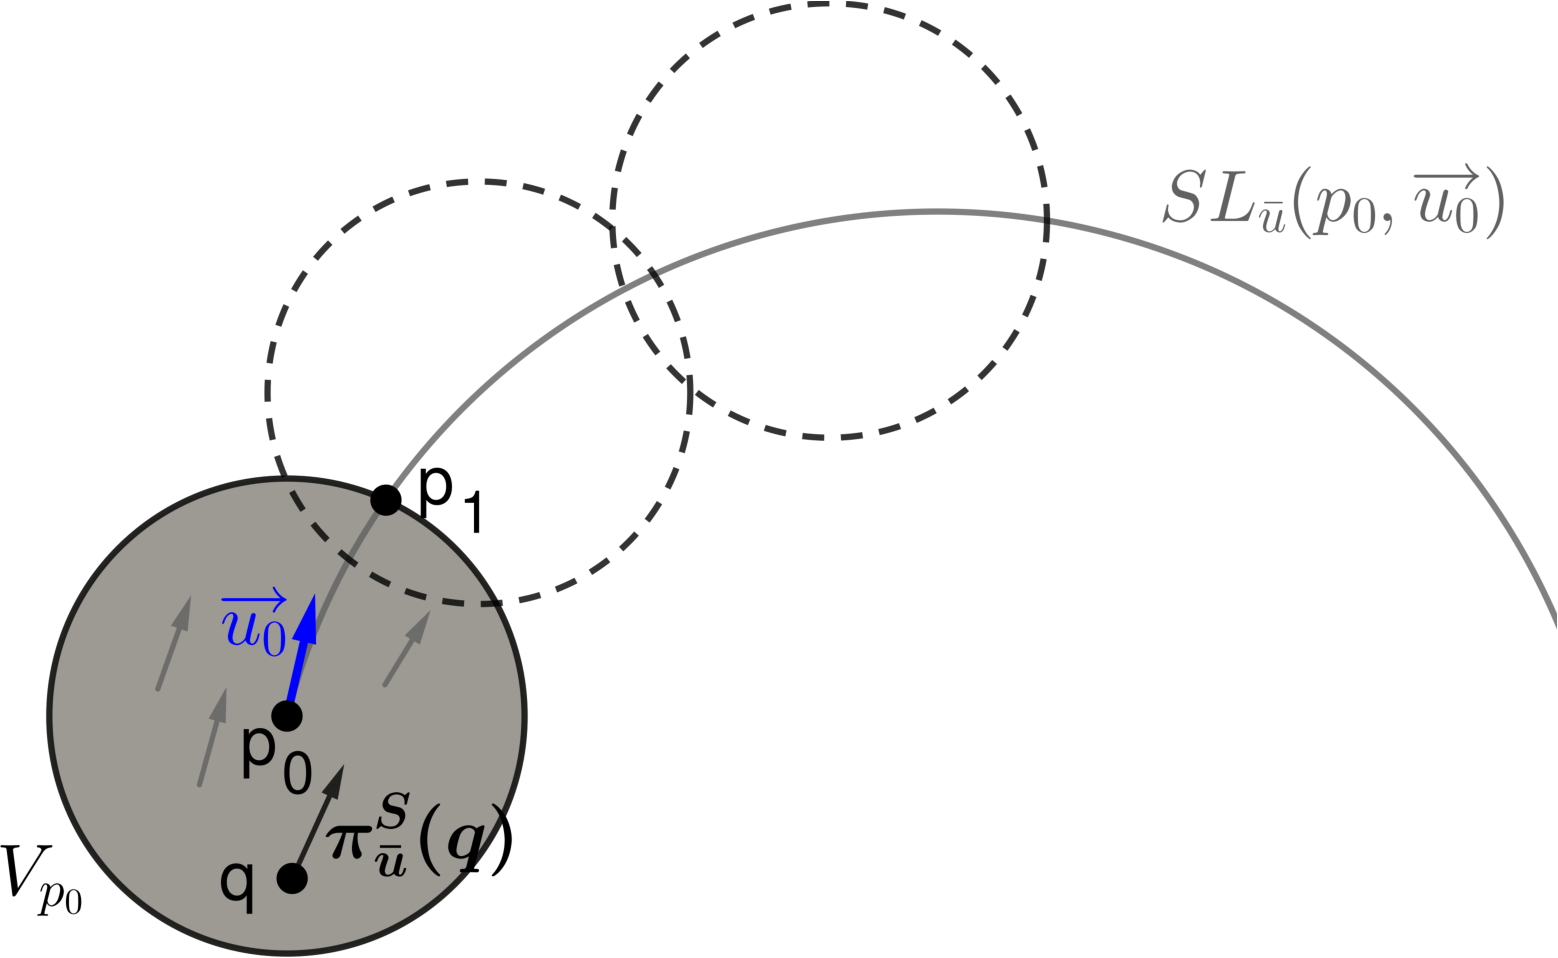
\includegraphics[scale=0.45]{images/streamline_construction.pdf}
\caption{Illustration de la preuve du lemme \ref{lem:def_streamline_lemma}.}
\label{fig:streamline_construction}
\end{figure}

\paragraph{Définition d'un champ de vecteur de classe $\mathcal{C}^1$ dans un voisinnage de $p_0$.} D'après la proposition \ref{prop:angular_cont}, il existe une application $\theta_{\bar{u}}^{V_{p_0}}$ de classe $\mathcal{C}^1$ dans un voisinnage $V_{p_0}$ de $p_0$ telle que pour tout $q\in V_{p_0}$, $\theta_{\bar{u}}^{V_{p_0}}(q)\equiv\theta_{\bar{u}}(q)\pmod{\frac{\pi}{2}}$. Il vient alors qu'il existe $m\in\mathbb{Z}$ tel que l'application $\tau_{p_0}:=\mathbf{R}(\theta_{\bar{u}}^{V_{p_0}}+m\frac{\pi}{2})(1, 0)$ est un champ de vecteur de classe $\mathcal{C}^1$ sur $V_{p_0}$ vérifiant $\tau_{p_0}(p_0)=\overrightarrow{u_0}$.

\paragraph{Construction de la restriction de $\pi_{\bar{u}}^S$ au voisinage de $p_0$.}
Montrons que si $\pi_{\bar{u}}^S\in\mathcal{C}^1(V_{p_0})$ tel que $\pi_{\bar{u}}^S(p_0)=\overrightarrow{u_0}$ satisfaisant \eqref{eqn:pi_u_S} et \eqref{eqn:streamline} alors $\pi_{\bar{u}}\circ S=\tau_{p_0}\circ S$ sur $V_{p_0}$. Supposons qu'il existe $t\in\mathbb{R}$ tel que $S(t)\in V_{p_0}$ et $\pi_{\bar{u}}^S\circ S(t)\neq\tau_{p_0}\circ S(t)$. Soit $\epsilon>0$ et notons $p'=S(t)$. $\tau_{p_0}$ étant continue sur $V_{p_0}$, on a:
$$|\tau_{p_0}(p')-\pi^S_{\bar{u}}(p_0)|=|\tau_{p_0}(p')-\tau_{p_0}(p_0)|\leq\epsilon.$$
Par inégalité triangulaire, il vient que:
$$|\pi^S_{\bar{u}}(p')-\pi^S_{\bar{u}}(p_0)|\geq|\tau_{p_0}(p')-\pi^S_{\bar{u}}(p')|-\epsilon.$$
Or on sait que $\pi^S_{\bar{u}}(p')\in{\bar{u}}(p')$, $\tau_{p_0}(p')\in{\bar{u}}(p')$ et $\pi_{\bar{u}}^S(p')\neq\tau_{p_0}(p')$, ce qui implique que $\pi^S_{\bar{u}}(p')=R(k\pi/2)\tau_{p_0}(p')$ où $k\in\mathbb{Z}\backslash 4\mathbb{Z}$, et donc que $|\pi^S_{\bar{u}}(p')-\tau_{p_0}(p')|\geq\sqrt{2}$. Par conséquent, on a:
$$|\pi^S_{\bar{u}}(p')-\pi^S_{\bar{u}}(p_0)|\geq|\sqrt{2}-\epsilon.$$
Ce qui contredit le fait que $\pi_{\bar{u}}^S\in\mathcal{C}^1(V_{p_0})$.


\paragraph{Construction de la restriction de la ligne de courant au voisinage de $p$.}
Selon ce qui a été établi précédemment, $S$ satisfait l'équation suivante dans $V_{p_0}$ :\begin{equation}
\label{eqn:streamline_in_V}
\frac{dS(t)}{dt}=\tau_{p_0}(S(t)),t\in \mathbb{R} \text{ et }  S(0)=p_0.
\end{equation}
Nous obtenons la séparatrice $S$ en intégrant l'équation \eqref{eqn:streamline_in_V} jusqu'à ce que $u(s(t))=0$ ou que $s(t)\in\partial V_{p_0}$ pour $t>0$ (respectivement, $t<0$). Sans perte de généralité, notons $t_1$ le moment auquel cela se produit et $S(t_1)=p_1$.\\
\begin{itemize}
\item[-] Si $\bar{u}(p_1)=0$, alors $S(t)$ est la ligne de champ construite existe et est unique,\\
\item[-] Sinon, nous pouvons étendre l'ensemble $S$ en répétant la construction précédemment décrite dans un voisinage de $p_1$. Cela implique de définir un champ vectoriel continu à proximité de $p_1$ et de construire la ligne de champ en fonction de ce champ étendu. En appliquant itérativement ce processus dans chaque voisinage, nous pouvons étendre et affiner progressivement la ligne de courant, en garantissant sa régularité dans tout le domaine.
\end{itemize}
\end{proof}


\begin{remark}
Notons que si $\bar{u}$ est aligné avec la frontière, alors pour tout $p\in \partial \Omega \backslash \mathcal{S}_{\bar{u}}$ tel que la normale extérieure unitaire $N(p)$ au point $p$, est définie, nous avons $SL{\bar{u}}\left(p,\mathbf{R}\left(\pm \frac{\pi}{2}\right)N(p)\right) \subset \partial \Omega$.
\end{remark}

\begin{definition}[Séparatrice] \label{def:sep}
Une séparatrice dans un champ de croix est une ligne de champ qui commence ou se termine en un point singulier.
\end{definition}

Cette définition d'une séparatrice induit un problème bien connu dans les équations différentielles ordinaires : comment tracer une ligne de champ à partir d'un point singulier donné ? Cette question peut être difficile étant donné que $\bar{u}(p)={0}$ pour tout $p\in \mathcal{S}_{\bar{u}}$. Cependant, nous proposons le résultat suivant qui sera utilisé par la suite pour contourner ce problème.
\begin{proposition}
\label{prop:stream_from_interior_sing}
Soit $\bar{u}$ un champ de croix presque-$\mathcal{C}^1$ et $p\in \Omega\backslash\partial\Omega$. Soit $V_p\subset\Omega$ un voisinnage de $p$ tel que le bord $\partial V_p$ de $V_p$ est de classe $\mathcal{C}^1$ et $\partial V_p\cap\mathcal{S}_{\bar{u}}=\emptyset$. On suppose de plus que $V_p$ est étoilé par rapport à $p$. Alors il existe un champ de croix $\bar{v}$ tel que:\\[-0.3cm]
\begin{enumerate}
\item $\bar{v}$ est presque-$\mathcal{C}^1$ sur $\Omega$,\\[-0.3cm]
\item $\mathcal{S}_{\bar{v}}\cap V_p =\{p\}$ et $id_{\bar{v}}(p)=\sum_{q\in \mathcal{S}_{\bar{u}}\cap V_p} id_{\bar{u}}(q)$,\\[-0.3cm]
\item pour tout $q\in \partial V_p$ tel que $\overrightarrow{v_q}:=\overrightarrow{pq}.\|\overrightarrow{pq}\|^{-1}\in \bar{u}(q)$, le point $p$ appartient à la ligne de champ $SL_{\bar{v}}(q,\overrightarrow{v_q})$.\\[-0.3cm]
\end{enumerate}
\end{proposition}

\begin{proof}
Soit $\bar{v}$ défini pour tout $q\in\Omega$ par :
\begin{equation}
\bar{v}(q)=
\left\{
\begin{array}{ll}
0&\mbox{ si }q=p\\[0.25cm]
\bar{u}(q)&\mbox{ si } q\notin V_p,\\[0.25cm]
\bar{u}\circ\pi(q)&\mbox{ sinon},
\end{array}
\right.
\end{equation}
où $\pi$ est défini pour tout $q\in V_p\backslash\{p\}$ par:
\begin{equation*}
\left\{
\begin{array}{ll}
\pi(q)=p+\displaystyle\frac{\overrightarrow{\|p\pi(q)\|}}{\overrightarrow{\|pq\|}}\overrightarrow{pq},\\[0.5cm]
\pi(q)\in\partial V_p.
\end{array}
\right.
\end{equation*}
Notons que $\pi$ est bien définie. En effet, puisque $V_p$ est étoilé et que $\partial V_p$ est de classe $\mathcal{C}^1$, alors pour tout $q\in V_p\backslash\{p\}$, il existe un unique point $\pi(q)\in\partial V_p$.\\\\
1.\quad Par définition $\bar{v}$ est presque-$\mathcal{C}^1$ dans $\Omega\backslash V_p$ et sur $\partial V_p$. Pour montrer que $\bar{v}$ est presque-$\mathcal{C}^1$ dans $V_p\backslash\{p\}$, il suffit de montrer que $\pi$ est $\mathcal{C}^1$ puisque $\bar{u}$ est $\mathcal{C}^1$ sur $\partial V_p$. Supposons que $\pi$ est $\mathcal{C}^1$. Soit $q\in V_p$ et $h\in\mathbb{R}^2$. Calculons $\pi(q+h)$.
\begin{eqnarray*}
    \pi(q+h)&=&p+\frac{\|\overrightarrow{p\pi(q+h)}\|}{\|\overrightarrow{p(q+h)}\|}\overrightarrow{p(q+h)}\\[0.2cm]
    &=&p+\left(\frac{\|\overrightarrow{p\pi(q)}\|}{\|\overrightarrow{pq}\|}+\frac{<\overrightarrow{p\pi(q)}, (\nabla\pi(q).h)>}{\|\overrightarrow{pq}\|\|\overrightarrow{p\pi(q)}\|}\right)\left(1-\frac{\overrightarrow{pq}.h}{\|\overrightarrow{pq}\|^2}\right)\left(\overrightarrow{pq}+h\right) + o(h^2)\\[0.2cm]
    &=&\pi(q)+\frac{<\overrightarrow{p\pi(q)}, (\nabla\pi(q).h)>}{\|\overrightarrow{pq}\|\|\overrightarrow{p\pi(q)}\|}\overrightarrow{pq}-\frac{\|\overrightarrow{p\pi(q)}\|}{\|\overrightarrow{pq}\|}\frac{\overrightarrow{pq}.h}{\|\overrightarrow{pq}\|^2}\overrightarrow{pq}+\frac{\|\overrightarrow{p\pi(q)}\|}{\|\overrightarrow{pq}\|}h+o(h^2)\\[0.2cm]
    \pi(q+h)&=&\pi(q)+\frac{<\overrightarrow{p\pi(q)}, (\nabla\pi(q).h)>}{\|\overrightarrow{pq}\|\|\overrightarrow{p\pi(q)}\|}\overrightarrow{pq}+\frac{\|\overrightarrow{p\pi(q)}\|}{\|\overrightarrow{pq}\|}\left(\frac{\overrightarrow{pq}.h}{\|\overrightarrow{pq}\|^2}\overrightarrow{pq}+h\right)+o(h^2)
\end{eqnarray*}

En posant $e_q=\displaystyle\frac{\overrightarrow{pq}}{\|\overrightarrow{pq}\|}$ et $\lambda_q=\displaystyle\frac{\|\overrightarrow{p\pi(q)}\|}{\|\overrightarrow{pq}\|}$ on obtient:

\begin{eqnarray*}
    \pi(q+h) = \pi(q)+<e_q,\nabla\pi(q).h>e_q+\lambda_q(-(e_q.h)e_q+h)+o(h^2)
\end{eqnarray*}
Posons $L(h)=<e_q,\nabla\pi(q).h>e_q+\lambda_q(-(e_q.h)e_q+h)$. La composante de $L(h)$ suivant $\overrightarrow{e_q^\perp}$ est donné par $X=L(h).e_q^\perp=\lambda_q(h.e_q^\perp)$. Nous cherchons ensuite la composante suivant $\overrightarrow{e_q}$: soit $\gamma$ une paramétrisation de $\partial V_p$ sur $I\subset\mathbb{R}$. Puisque $\pi(q+h),\pi(q)\in\partial V_p$, il existe $t_1, t_2\in I$ tel que $\pi(q)=\gamma(t_1)$ et $\pi(q+h)=\gamma(t_2)$. $\gamma$ étant $\mathcal{C}^1$, il existe une fonction dépendant de $h$ noté $m(h)$ tel que $\pi(q+h)-\pi(q)=m(h).\overrightarrow{t}+o(h^2)$ avec $\overrightarrow{t}=\gamma'(t_1).\|\gamma'(t_1)\|^{-1}$. Ce qui implique que $L(h)$ est colinéaire au vecteur $\overrightarrow{t}$. Il vient alors que:
$$
\|L(h)\|=\frac{X}{\cos{\alpha}},\mbox{ avec }\cos{\alpha}=\overrightarrow{t}.\overrightarrow{e_q^\perp}
$$
Autrement dit, la composante de $L(h)$ suivant $e_q$ noté $Y$ est donné par:
$$
Y=\sqrt{\|L(h)\|^2-X^2}=\frac{1}{\cos{\alpha}}\sqrt{X^2(1+\cos^2\alpha)}
$$
\begin{comment}
\begin{figure}[!h]
\centering
\includegraphics[scale=0.4]{img/im_future.png}
\caption{}%Illustration de la construction de la restriction de $\pi$.}
%\label{fig:v_bar_almost_continuous}
\end{figure}
\end{comment}
Finalement, on a $L(h)=X\overrightarrow{e_q^\perp}+ Y\overrightarrow{e_q}$ avec $X$ et $Y$ linéaire et continue. Par conséquent, $\pi$ est bien de classe $\mathcal{C}^1$.\\\\
2.\quad Pour tout $q\in V_p\backslash\{p\}$, $\bar{v}(q)\neq 0$ et $\bar{v}(p)=0$. Par conséquent, $\mathcal{S}_{\bar{v}}\cap V_p=\{p\}$. Soit $\gamma$ une paramétrisation de $\partial V_p$ sur $[0, 1]$. Sachant que l'indice de $p$ dans le champ de croix $\bar{v}$ ne dépend pas du chemin, on peut écrire que:
$$id_{\bar{v}}(p)=\frac{1}{2\pi}\int_{\partial V_p}d\theta_{\bar{v}}.$$
Or par construction, on a $\bar{v}=\bar{u}$ sur $\partial V_p$ donc on a:
$$id_{\bar{v}}(p)=\frac{1}{2\pi}\int_{\partial V_p}d\theta_{\bar{u}}=\sum_{q\in\mathcal{S}_{\bar{u}}\cap V_p}id_{\bar{u}}(q).$$\\\\
3.\quad Soit $q\in\partial V_p$ tel que $\overrightarrow{v_q}:=\overrightarrow{pq}.\|\overrightarrow{pq}\|^{-1} \in \bar{u}(q)$. Alors pour tout $p'\in~]pq)\cap V_p$ on a $\overrightarrow{v_q}\in\bar{v}(p')$. Par conséquent, pour tout $p'\in]pq]$ on a $p'\in SL_{\bar{v}}(q,\overrightarrow{v_q})$. Ainsi en passant à la limite avec $p'\longrightarrow p$ on a $p\in SL_{\bar{v}}(q,\overrightarrow{v_q})$.
\end{proof}

En extension de la proposition \ref{prop:stream_from_interior_sing}, nous introduisons la proposition suivante, qui décrit une procédure pour tracer une ligne de courant à partir d'un point singulier spécifié sur la frontière.

\begin{proposition}
\label{prop:stream_from_bord_sing}
Soit $\bar{u}$ un champ de croix presque-$\mathcal{C}^1$ et $p\in\partial\Omega$. Considérons un voisinage $V_p\subset\Omega$ de $p$ tel que $p\in\partial V_p$ et $\partial V_p$ soit de classe $\mathcal{C}^1$. On suppose de plus que $(\partial V_p\backslash\{p\})\cap\mathcal{S}_{\bar{u}}=\emptyset$ et que $V_p$ est étoilé par rapport à $p$. Alors, il existe un champ de croix $\bar{v}$ tel que:
\begin{enumerate}
\item[1.] $\bar{v}$ est presque-$\mathcal{C}^1$ sur $\Omega$,\\[-0.3cm]
\item[2.] pour tout $q\in \partial V_p$ tel que $\overrightarrow{v_q}:=\overrightarrow{pq}.\|\overrightarrow{pq}\|^{-1}\in \bar{u}(q)$, le point $p$ appartient à la ligne de champ $SL_{\bar{v}}(q,\overrightarrow{v_q})$.\\[-0.3cm]
\end{enumerate}
De plus, si $\partial V_p$ est tangent à $\partial\Omega$ en p, alors on a:
\begin{enumerate}
\item[3.] $\mathcal{S}_{\bar{v}}\cap V_p =\{p\}$ et $id^\partial_{\bar{v}}(p)=\sum_{q\in \mathcal{S}_{\bar{u}}\cap V_p} id_{\bar{u}}(q)$.\\[-0.3cm]
\end{enumerate}
\end{proposition}

\begin{proof}
Soit $\bar{v}$ défini pour tout $q\in\Omega$ par :
\begin{equation}
\bar{v}(q)=
\left\{
\begin{array}{ll}
0&\mbox{ si }q=p\\[0.25cm]
\bar{u}(q)&\mbox{ si } q\notin V_p,\\[0.25cm]
\bar{u}\circ\pi(q)&\mbox{ sinon},
\end{array}
\right.
\end{equation}
où $\pi$ est défini pour tout $q\in V_p\backslash\{p\}$ par:
\begin{equation*}
\left\{
\begin{array}{ll}
\pi(q)=p+\displaystyle\frac{\overrightarrow{\|p\pi(q)\|}}{\overrightarrow{\|pq\|}}\overrightarrow{pq},\\[0.5cm]
\pi(q)\in\partial V_p.
\end{array}
\right.
\end{equation*}
Notons que $\pi$ est bien définie. En effet, puisque $V_p$ est étoilé et que $\partial V_p$ est de classe $\mathcal{C}^1$, alors pour tout $q\in V_p\backslash\{p\}$, il existe un unique point $\pi(q)\in\partial V_p$.\\\\
1.\quad De manière analogue à la preuve de la proposition \ref{prop:stream_from_bord_sing} on montre que $\bar{v}$ est presque-$\mathcal{C}^1$ sur $\Omega$.\\\\
2.\quad Soit $q\in\partial V_p$ tel que $\overrightarrow{v_q}:=\overrightarrow{pq}.\|\overrightarrow{pq}\|^{-1} \in \bar{u}(q)$. Alors pour tout $p'\in~]pq)\cap V_p$ on a $\overrightarrow{v_q}\in\bar{v}(p')$. Par conséquent, pour tout $p'\in]pq]$ on a $p'\in SL_{\bar{v}}(q,\overrightarrow{v_q})$. Ainsi en passant à la limite avec $p'\longrightarrow p$ on a $p\in SL_{\bar{v}}(q,\overrightarrow{v_q})$.\\\\
3.\quad Supposons maintenant que $\partial V_p$ est tangent à $\partial V_p$ en p. Pour tout $q\in V_p\backslash\{p\}$, $\bar{v}(q)\neq 0$ et $\bar{v}(p)=0$. Par conséquent, $\mathcal{S}_{\bar{v}}\cap V_p=\{p\}$. Soit $\gamma$ une paramétrisation de $\partial V_p$ sur $[0, 1]$ avec $\gamma(0)=p=\gamma(1)$. Puisque $\partial V_p$ est tangent à $\partial\Omega$ en p, les vecteurs $\gamma'(0)$ et $\gamma'(1)$ sont tangents à $\partial\Omega$. On a donc:
$$
id^\partial_{\bar{v}}(p)=\frac{1}{2\pi}\left[\pi-\hat{p}+\lim\limits_{s\rightarrow 0}\int_s^{1-s}d\theta_{\bar{v}}^\gamma\right]
$$
Or par construction, on a $\bar{v}=\bar{u}$ sur $\partial V_p$ donc on a:
$$id^\partial_{\bar{v}}(p)=\frac{1}{2\pi}\left[\pi-\hat{p}+\lim\limits_{s\rightarrow 0}\int_s^{1-s}d\theta_{\bar{u}}^\gamma\right]=\sum_{q\in\mathcal{S}_{\bar{u}}\cap V_p}id_{\bar{u}}(q).$$

\end{proof}


\begin{comment}
Dans la suite de ce travail, nous faisons systématiquement correspondre un champ de croix donné avec un champ reconstruit obtenu en applicant la construction donnée dans les propositions \ref{prop:stream_from_interior_sing} et \ref{prop:stream_from_bord_sing}, en utilisant la même notation pour les deux (le champ et sa reconstruction) afin de ne pas alourdir la présentation. Ainsi étant donné un champ de croix $\bar{u}$ presque-$\mathcal{C}^1$ sur $\Omega$, nous adoptons les notations suivantes : pour tout point $p\in\mathcal{S}_{\bar{u}}$, nous notons $V_p^*$ le voisinage dans lequel le champ a été reconstruit, et $\gamma$ une paramétrisation sur $[0, 1]$ de $\partial V_p^*$ dans le sens anti-horaire.
\end{comment}

D'après les propositions \ref{prop:stream_from_interior_sing} et \ref{prop:stream_from_bord_sing}, pour tracer une séparatrice à partir d'un point singulier dans un champ de croix, il est nécessaire de disposer d'un vecteur dont le point d'application coïncide avec le point singulier en question et qui est aligné avec le champ de croix dans un voisinage de ce point singulier. Voisinnage dans lequel le champ a préalablement été modifié grâces aux propositions \ref{prop:stream_from_interior_sing} et \ref{prop:stream_from_bord_sing}. La question qui se pose alors est de savoir si de tels vecteurs existent, et combien de ces vecteurs sont disponibles pour chaque point singulier. Autrement dit, on cherche à déterminer combien de séparatrices peuvent être associées à un point singulier donné, ainsi que leurs orientations initiales. Nous exposons ci-après plusieurs résultats permettant de répondre à cette problématique.

Dans ce qui suit, nous adopterons les notations suivantes. \'Etant donné $p\in\Omega$ nous désignons par $V_p\subset\Omega$ un voisinnage de $p$ tel que le bord $\partial V_p$ de $V_p$ est de classe $\mathcal{C}^1$ et $\partial V_p\cap\mathcal{S}_{\bar{u}}=\emptyset$. Soit $\gamma$ une paramétrisation sur $[0, 1]$ dans le sens positif de $\partial V_p$. Nous désignons par $W_p^\gamma$ la fonction définie par:
\begin{equation}
\label{eqn:Winding}
W_p^\gamma:t\in[0, 1]\longmapsto \theta^\gamma_{\bar{u}}(t)-\arg \overrightarrow{p\gamma(t)},
\end{equation}
qui indique la différence angulaire relative entre le champ de croix et le champ radial au point $p$ (où $\arg \overrightarrow{p\gamma(t)}$ désigne l'argument complexe de $\overrightarrow{p\gamma(t)}$).

\begin{remark}
\label{rmk:W_p_gamma}
La définition de $W_p^\gamma$ dépend du choix de $\theta_{\bar{u}}^\gamma$ donné par le Corollaire \ref{cor:relevement_continu}, qui n'est pas unique mais est défini à une constante près de $m\pi/2$ avec $m\in\mathbb{Z}$. Cela signifie que différents choix de $\theta_{\bar{u}}^\gamma$ peuvent conduire à différentes valeurs de $W_p^\gamma$, mais ils diffèrent seulement par un multiple de $\pi/2$ ce qui n'aura pas d'impact sur ce qui suit.
\end{remark}

\begin{lemma}
\label{lem:decoup_voisinnage}
Soit $p\in\Omega\backslash\partial\Omega$ tel que $id_{\bar{u}}(p)=k/4$ avec $k\in\mathbb{Z}$ et $k\leq 1$. Pour tout $t_0\in[0, 1]$, on a:\\

\begin{itemize}
    \item[$\bullet$] $\exists (t_i)_{i\in\llbracket1, N_s\rrbracket}\subset[0, 1]$ tel que $N_s=4-k$ et $0\leq t_1<\dots< t_{N_s}\leq 1$,\\
    \item[$\bullet$] $\exists i\in [0, 1]$ tel que $t_0=t_i$, et pour tout $i\in\llbracket 1, N_s\rrbracket$,
$$\int_{t_i}^{t_{i+1}}dW_p^\gamma=-\frac{\pi}{2},\mbox{ où }t_{N_s+1}:=t_1.$$
\end{itemize}
\end{lemma}

\begin{proof}
Étant donné que $id_{\bar{u}}(p)=k/4$, on a:
$$\int_0^1 d\theta^\gamma_{\bar{u}}=k\frac{\pi}{2}$$
Or on a $\int_0^1 d\arg{\overrightarrow{p\gamma(t)}}=2\pi$ donc:
$$\int_0^1 dW_p^\gamma=(k-4)\frac{\pi}{2}=-N_s\frac{\pi}{2} \mbox{ avec } N_s=4-k.$$
Définissons maintenant une fonction $h: t \mapsto h(t) \in \mathbb{R}$ comme suit :
$$
h(t) =
    \begin{cases}
        t&\mbox{ for }t\in[t_0, 1], \\
        t+1&\mbox{ for }t\in[0,t_0[.
    \end{cases}
$$
Il vient alors que:
$$\int_0^1 dW_p^\gamma(t)=\int_{t_0}^{t_0+1} d(W_p^\gamma \circ h).$$
Posons $t'_1 := t_0$ et définissons la fonction $f$ par:
$$f: \tau \mapsto \int_{t'_1}^\tau d(W_p^\gamma \circ h).$$
Comme $f$ est continue sur $[0,1]$, l'application du théorème des valeurs intermédiaires, conduit à l'existence de $(t'_i)_{i\in\llbracket 2,N_s\rrbracket}\subset[0, 1]$ tels que $t'_1<t'_2<\dots<t'_{N_s}$ et pour tout $i\in\llbracket1, N_s\rrbracket$ on a:
$$\int_{t'_i}^{t'_{i+1}}d(W_p^\gamma\circ h)=-\frac{\pi}{2},$$
où $t'_{N_s+1}:=t'_1$. Enfin, nous pouvons définir $t_i=h^{-1}(t'_i)$ pour tout $i\in\llbracket 1,N_s\rrbracket$, ce qui donne une suite de $N_s=4-k$ points $0\leq t_1\leq\dots\leq t_{N_s}\leq 1$ tels que $\exists i\in\llbracket 1,N_s\rrbracket$ avec $t_i=t_0$. De plus, $\forall i\in\llbracket 1,N_s\rrbracket$, nous avons:
$$\int_{t_i}^{t_{i+1}}dW_p^\gamma=-\frac{\pi}{2},\mbox{ où }t_{N_s+1}:=t_1.$$
\end{proof}

En se basant sur ce résultat, nous sommes en mesure d'énoncer la proposition suivante, laquelle permet de déterminer le nombre de séparatrices à attribuer à un point singulier ainsi que leur orientation initiale.

\begin{proposition}
    \label{prop:align_sepa_voisinnage}
    Soit $p\in\Omega\backslash\partial\Omega$ tel que $id_{\bar{u}}(p)=k/4$ avec $k\in\mathbb{Z}$ et $k\leq 1$. Pour tout $t_0\in[0, 1]$, il existe une suite de points $(t_i)_{i\in\llbracket1, N_s\rrbracket}$ tel que $N_s=4-k$ et $0\leq t_1\leq\dots\leq t_{N_s}\leq 1$ avec $\overrightarrow{p\gamma(t_i)}.\|\overrightarrow{p\gamma(t_i)}\|^{-1}\in\bar{u}(\gamma(t_i))$. De plus, il existe $i\in [0, 1]$ tel que $t_i=t_0$, et pour tout $i\in\llbracket 1, N_s\rrbracket$,
    $$\int_{t_i}^{t_{i+1}}dW_p^\gamma=-\frac{\pi}{2},\mbox{ où }t_{N_s+1}:=t_1.$$
\end{proposition}

Selon la Remarque \ref{rmk:W_p_gamma}, il est en effet correct que $W_p^\gamma$ n'est pas unique et peut être défini à une constante près de $m\pi/2,~m\in\mathbb{Z}$. Cependant, dans le contexte du lemme \ref{lem:decoup_voisinnage}, nous pouvons observer que les valeurs de $t_i,~\forall i\in\llbracket 1, N_s\rrbracket$ données ne dépendent pas du choix spécifique de $W_p^\gamma$.

\begin{proof}
Selon le lemme \ref{lem:decoup_voisinnage}, s'il existe $t_0\in[0, 1]$ tel que $\overrightarrow{u_0}=\overrightarrow{p\gamma(t_0)}.\|\overrightarrow{p\gamma(t_0)}\|^{-1}\in\bar{u}(\gamma(t_0))$, alors il existe une suite de points $(t_i)_{i\in\llbracket1, N_s\rrbracket}$ tel que $N_s=4-k$ et $0\leq t_1\leq\dots\leq t_{N_s}\leq 1$. De plus, il existe $i\in [0, 1]$ tel que $t_i=t_0$, et pour tout $i\in\llbracket 1, N_s\rrbracket$,
$$\int_{t_i}^{t_{i+1}}dW_p^\gamma=-\frac{\pi}{2},\mbox{ où }t_{N_s+1}:=t_1.$$
Remarquons alors que pour tout $i\in\llbracket 1, N_s\rrbracket$, nous avons:$$\overrightarrow{u_i}=\overrightarrow{p\gamma(t_i)}.\|\overrightarrow{p\gamma(t_i)}\|^{-1}\in\bar{u}(\gamma(t_i)).$$
Cela peut être démontré de manière itérative comme suit: puisque $\int_{t_{i-1}}^{t_{i}}dW_p^\gamma=-\frac{\pi}{2}$ alors $\theta^\gamma_{\bar{u}}(t_i)=\arg \overrightarrow{p\gamma(t_i)} +\theta^\gamma_{\bar{u}}(t_{i-1})-\arg \overrightarrow{p\gamma(t_{i-1})}-\frac{\pi}{2}$. Étant donné que $\overrightarrow{p\gamma(t_{i-1})}.\|\overrightarrow{p\gamma(t_{i-1})}\|^{-1}\in\bar{u}(\gamma(t_{i-1}))$, on a $\theta^\gamma_{\bar{u}}(t_{i-1})\equiv\arg \overrightarrow{p\gamma(t_{i-1})}\pmod{\frac{\pi}{2}}$. Par conséquent, on peut en déduire que $\theta^\gamma_{\bar{u}}(t_{i})\equiv\arg \overrightarrow{p\gamma(t_i)}\pmod{\frac{\pi}{2}}$, ce qui prouve que $\overrightarrow{p\gamma(t_i)}.\|\overrightarrow{p\gamma(t_i)}\|^{-1}\in\bar{u}(\gamma(t_i))$.

Pour compléter la preuve, on doit montrer qu'il existe $t_0\in[0,1]$ tel que $\overrightarrow{p\gamma(t_0)}.\|\overrightarrow{p\gamma(t_0)}\|^{-1}\in\bar{u}(\gamma(t_0))$. Soit $s_0\in[0,1]$ tel que $0<W_p^\gamma(s_0)<\frac{\pi}{2}$. D'après le lemme \ref{lem:decoup_voisinnage}, il existe $s_1>s_0$ tel que $\int_{s_0}^{s_1}dW_p^\gamma=-\frac{\pi}{2}$, ce qui signifie que $W_p^\gamma(s_1)=W_p^\gamma(s_0)-\frac{\pi}{2}<0$. Par le théorème des valeurs intermédiaires, il existe donc $t_0\in[s_0, s_1]$ tel que $W_p^\gamma(t_0)=0$, ce qui implique que $\arg\overrightarrow{p\gamma(t_0)}\in\bar{u}(\gamma(t_0))$. Par conséquent, $\overrightarrow{p\gamma(t_0)}.\|\overrightarrow{p\gamma(t_0)}\|^{-1}\in\bar{u}(\gamma(t_0))$, ce qui complète la preuve.
\end{proof}

Ce résultat peut être étendu à un point de bord de la manière suivante:

\begin{proposition}
\label{prop:align_sepa_voisinnage_bord}
Soit $p\in\partial\Omega$ tel que $id_u(p)=k/4$ avec $k\in\mathbb{Z}$ et $k\leq 1$. Au point $p$, il y a $N_s=3-k$ séparatrices qui convergent, incluant les frontières de $\Omega$, divisant ainsi le voisinage de $p$ en $2-k$ secteurs. De plus, à l'intérieur de chaque secteur, on a:
$$\int_0^1W_p^\gamma(t)dt=-\frac{\pi}{2}.$$
\end{proposition}

\begin{proof}
Étant donné que $id_u(p)=k/4$, en utilisant l'équation \eqref{eqn:Indexboundary}, on a:
\begin{eqnarray*}
    \lim\limits_{s\rightarrow 0}\displaystyle\int_s^{1-s} dW_p^\gamma&=&\frac{k\pi}{2}+\hat{p}-\pi-\hat{p}\\
    &=&(k-2)\frac{\pi}{2}=-(N_s-1)\frac{\pi}{2},
\end{eqnarray*}
et donc $N_s=3-k$.
\begin{itemize}
\item Si $k=1$, alors $\lim\limits_{s\rightarrow 0}\displaystyle\int_s^{1-s} dW_p^\gamma= -\frac{\pi}{2}$. En conséquence, on observe l'existence d'un seul secteur.\vspace{0.1cm}
\item Sinon, si $k<1$. Selon le théorème des valeurs intermédiaires :\vspace{0.1cm}
\begin{itemize}
\item[-] Pour $k=0$, il existe $t_1\in]0, 1[$ tel que :
$$\lim\limits_{s\rightarrow 0}\displaystyle\int_s^{t_1} dW_p^\gamma= -\frac{\pi}{2} \mbox{ et } \lim\limits_{s\rightarrow 0}\displaystyle\int_{t_1}^{1-s} dW_p^\gamma= -\frac{\pi}{2}.$$
Par conséquent, on observe l'existence de 2 secteurs.\vspace{0.1cm}
\item[-] Pour $k=-1$, il existe $t_1$ et $t_2$ dans $]0, 1[$, $t_1<t_2$ tels que :
$$\lim\limits_{s\rightarrow 0}\displaystyle\int_s^{t_1} dW_p^\gamma= -\frac{\pi}{2},~ \int_{t_1}^{t_2}dW^\gamma_p=-\frac{\pi}{2} \mbox{ et } \lim\limits_{s\rightarrow 0}\displaystyle\int_{t_2}^{1-s} dW_p^\gamma= -\frac{\pi}{2}.$$\\\vspace{0.1cm}
\item[-] Pour $k<0$, il existe $(t_i)_{i\in\llbracket2, N_s\rrbracket}$, avec $0<t_1\leq\dots\leq t_{-k+1}<1$ tels que :
%\small
$$\lim\limits_{s\rightarrow 0}\displaystyle\int_s^{t_1} dW_p^\gamma= -\frac{\pi}{2},~ \lim\limits_{s\rightarrow 0}\displaystyle\int_{t_2}^{1-s} dW_p^\gamma= -\frac{\pi}{2} \mbox{ and } \int_{t_1}^{t_{-k+1}}dW^\gamma_p=\sum_{i=1}^{-k}\displaystyle\int_{t_i}^{t_{i+1}} dW_p^\gamma,$$
où $\forall i\in\llbracket 1, -k\rrbracket, \displaystyle\int_{t_i}^{t_{i+1}} dW_p^\gamma=-\frac{\pi}{2}.$
%\normalsize
Par conséquent, nous observons l'existence de $2-k$ secteurs.
La fonction $t\longmapsto\displaystyle\int_{t_1}^t dW_p^\gamma\in\mathcal{C}^0([0,1])$ implique, selon le théorème des valeurs intermédiaires, l'existence de $(t_i)_{i\in\llbracket2, -k+1\rrbracket}\subset[0, 1]$ tels que $\displaystyle\int_{t_1}^{t_f} dW_p^\gamma=\sum_{i=1}^{-k}\displaystyle\int_{t_i}^{t_{i+1}}dW_p^\gamma$ où $\displaystyle\int_{t_i}^{t_{i+1}}dW_p^\gamma=-\frac{\pi}{2},~\forall i\in\llbracket1, N_s\rrbracket$ et $t_{N_s+1}:=t_1$.
Grâce au théorème des valeurs intermédiaires, il existe $t_i$ tel que :
$$\displaystyle\int_{t_1}^{t_f} dW_p^\gamma= \sum_{i=1}^{-k}\displaystyle\int_{t_i}^{t_{i+1}} dW_p^\gamma \mbox{ with } \displaystyle\int_{t_i}^{t_{i+1}} dW_p^\gamma=-\frac{\pi}{2}\mbox{ and } t_f=t_{-k+1}.$$
\end{itemize}
\end{itemize}
\end{proof}
La figure \ref{fig:separatrice_illustration} illustre le partitionnement du voisinnages de points singulier par les séparatrices issues de ces points singuliers. En effet, en fonction de l'index du point ces séparatrices divisent le voisinnage du point en un nombre fini de de secteur. Par rapport à ces secteurs, nous avons la proposition suivante:
\begin{figure}[!h]
  \centering
  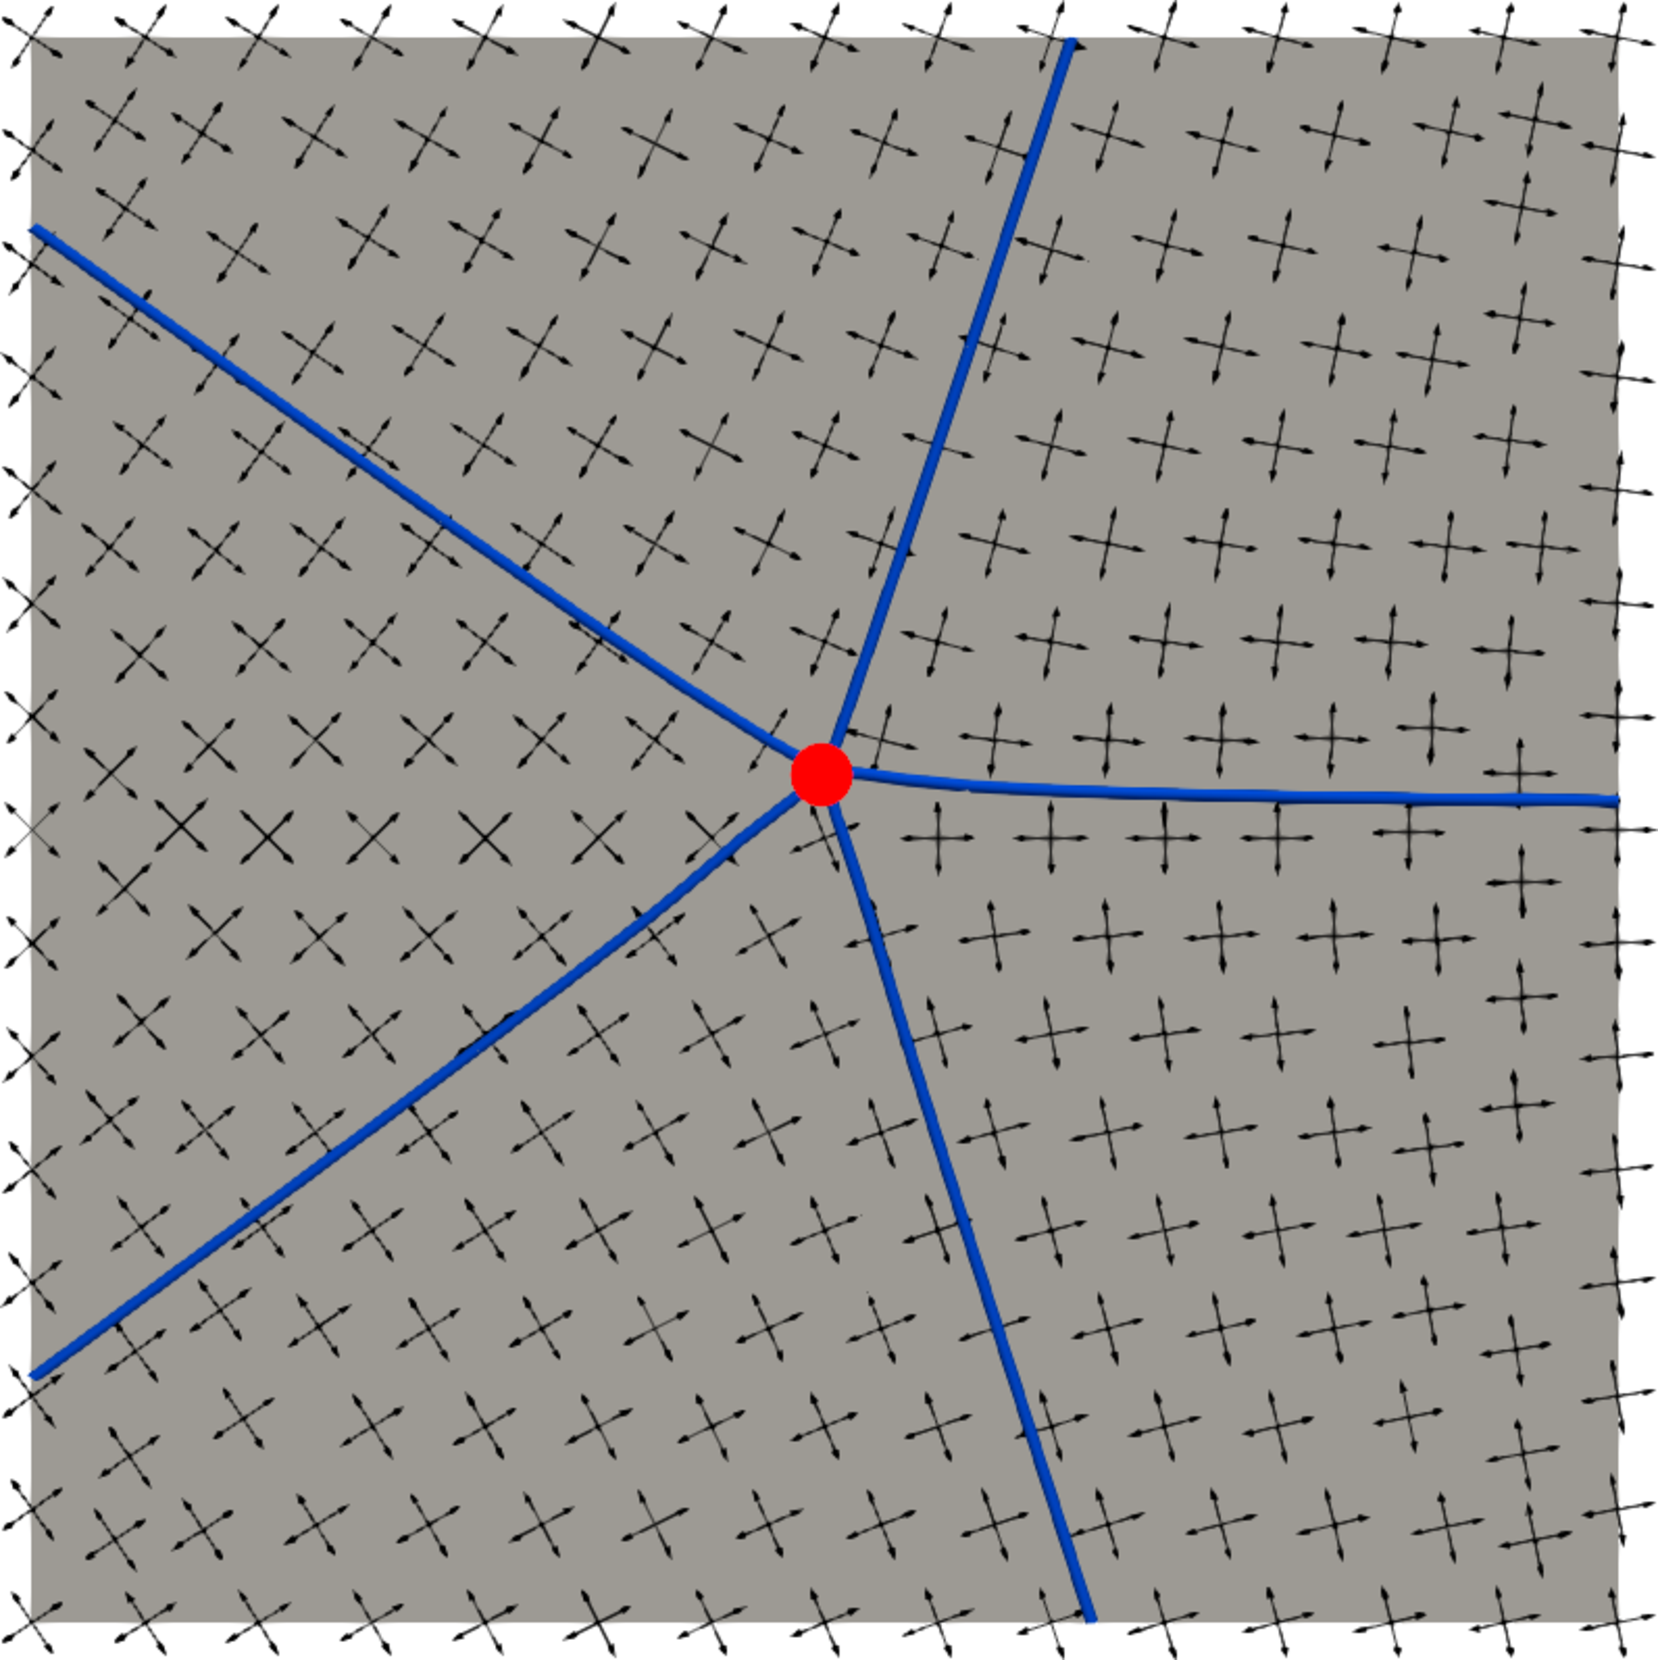
\includegraphics[scale=0.27]{images/sepa_5.pdf}\hspace{0.2cm}
  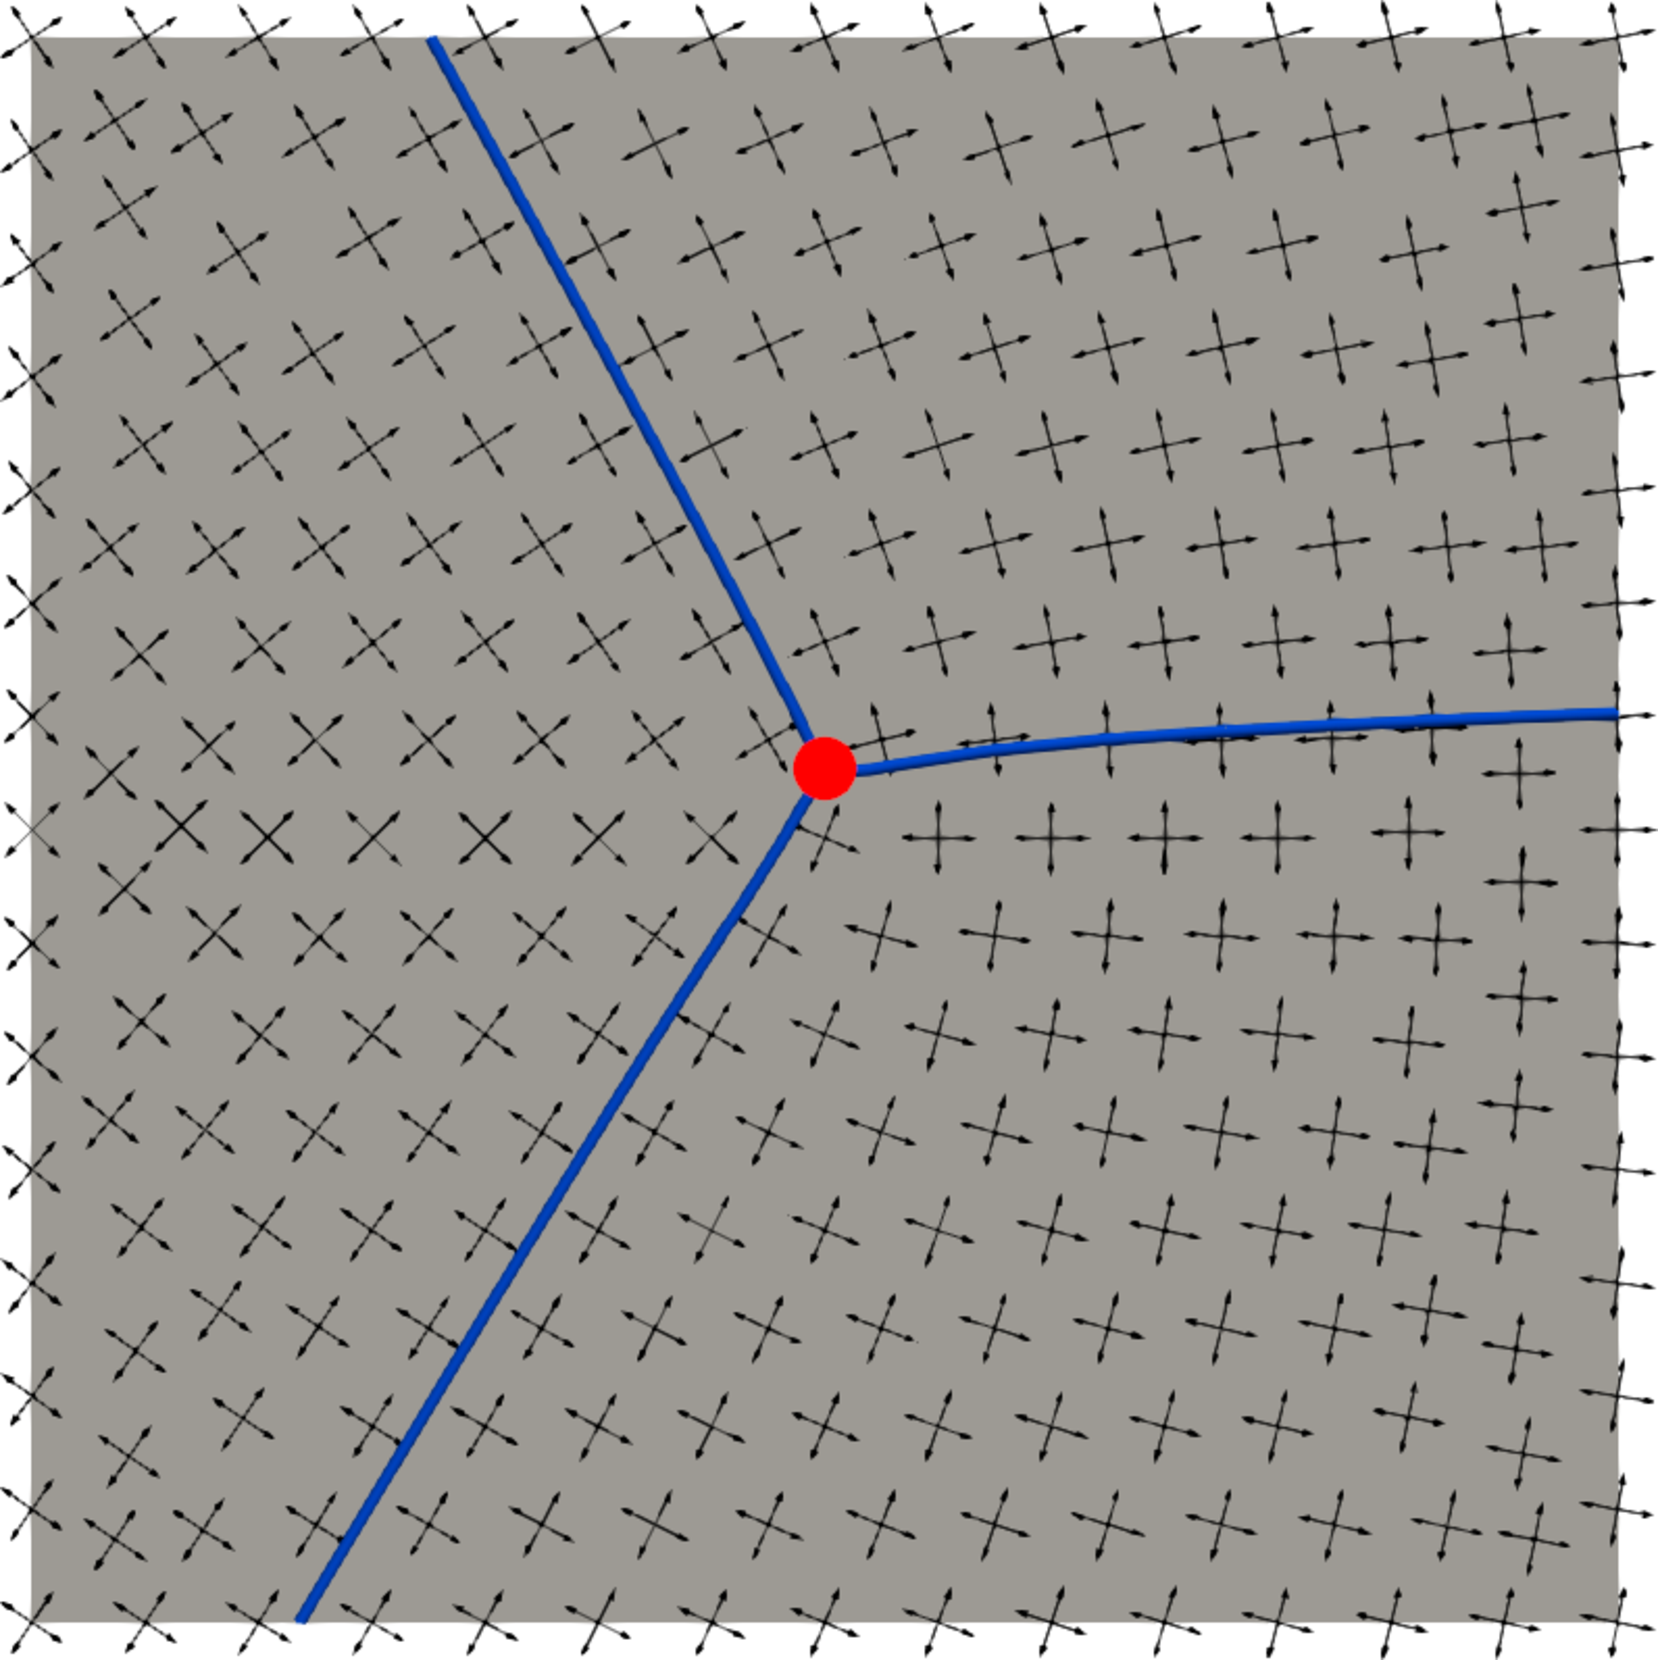
\includegraphics[scale=0.27]{images/sepa_3.pdf}
  \caption{Gauche: Illustration des séparatrices émanant de points singuliers d'indice $-1/4$ (à gauche) et d'indice $1/4$ (à droite).}
  \label{fig:separatrice_illustration}
\end{figure}

\begin{proposition}
\label{prop:loveprop}
Considérons un secteur tel que décrit ci-dessus. Lorsqu'il est traité comme une singularité de bord du secteur, le point $p$ a un indice de $1/4$.
\end{proposition}

\begin{proof}
Supposons que le secteur soit défini par deux séparatrices avec des directions initiales $\overrightarrow{p\gamma(t_i)}$ et $\overrightarrow{p\gamma(t_{i+1})}$, qui sont alignées avec la frontière du secteur. Soit $C$, la paramétrisation de la courbe définie par $p\gamma(t_i)$, $p\gamma(t_{i+1})$ et la partie de $\gamma$ coincé dans le secteur. L'indice de $p$ est alors donné par:
\begin{eqnarray*}
id^\partial_{\bar{u}}(p)&=&\frac{1}{2\pi}\left[\pi-\hat{p}+\lim\limits_{s\rightarrow 0}\int_{s-t_i}^{s-t_{i+1}}d\theta_{\bar{u}}^\gamma\right]\\
&=&\frac{1}{2\pi}\left[\pi-\hat{p}+\left(\hat{p}+\lim\limits_{s\rightarrow 0}\int_{s-t_i}^{s-t_{i+1}}dW_p^\gamma\right)\right]\\
&=&\frac{1}{2\pi}\left[\pi-\frac{\pi}{2}\right]\\
id^\partial_{\bar{u}}(p)&=&\frac{1}{4}.
\end{eqnarray*}
\end{proof}

De manière analogue à ce qui est fait dans \cite{viertel2019approach}, la proposition \ref{prop:loveprop} implique que l'apparence de chaque coin d'un secteur est celle d'un angle droit par rapport au champ de croix.

\begin{comment}
\[\]
commentaires sur les secteurs\\
on retrouve ici la notion de valence évoqué dans l'introduction.
un point sera dit régulier si Ns= autrement dit si id=
reprendre les dessin sur l'illustration des index, tracer les sepatrices pour visulaiser ce qu'est un secteur.
\end{comment}


\section{Méthode de partitionnement à partir d'un champ de croix}

Nous abordons maintenant le cœur de ce chapitre en présentant la méthode de partitionnement de domaine basée sur les champs de croix. Dans un premier temps, nous exposons l'algorithme de partitionnement ainsi que les différentes conditions requises sur le champ de croix, garantissant ainsi que le partitionnement obtenu résulte en un maillage quadrilatéral du domaine de départ. Par la suite, nous analysons en détail les différents algorithmes présentés et fournissons des résultats permettant de garantir leur bon fonctionnement.

\subsection{Principe de la méthode}
\label{subsec:principe_methode}

Considérons un domaine $\Omega$ borné et fermé dans $\mathbb{R}^2$ possédant une frontière $\partial\Omega$ régulière par morceaux. L'algorithme suivant permet de partitionner ce domaine en régions distincts.\\

\RestyleAlgo{ruled}

\begin{algorithm}[H]
\label{alg:algo_main}
\SetKwInOut{Input}{Entrée}
\SetKwInOut{Output}{Sortie}
\Input{$\Omega$ un domaine borné et fermé; Un champ de croix presque-$\mathcal{C}^1$ défini sur $\Omega$ est tel que l'indice des points dans ce champ est égal à $k/4$, où $k\in\mathbb{Z}$ et $k\leq 1$.}
\Output{Partition de $\Omega$ en ensembles de régions.}
\vspace{0.2cm}
1.) Identification des points singuliers du champ de croix,\\\vspace{0.2cm}
2.) Détermination du nombre de séparatrices pour chaque point singulier,\\\vspace{0.2cm}
3.) Intégration des séparatrices,\\\vspace{0.2cm}
4.) Identification des régions.\\\vspace{0.2cm}
\caption{Algorithme de partitionnement}
\end{algorithm}
\vspace{0.5cm}
On considère que l'algorithme a convergé si les séparatrices ne convergent pas vers un cycle limite. Examinons en détail les différentes étapes de cet algorithme pour en comprendre les nuances et les implications:
\vspace{0.5cm}

\begin{enumerate}
\item \textbf{Identification des points singuliers :} l'algorithme commence par identifier les points singuliers dans le champ de croix fourni. Ces points singuliers jouent un rôle critique dans la détermination de la structure du maillage. Ils correspondent à des points $p\in\Omega$, tels que $\bar{u}(p)=0$ (voir la première image de la figure \ref{fig:demi_disc_align_first}).\\
\item \textbf{Détermination du nombre de séparatrices pour chaque point singulier :}
le nombre de lignes de champ provenant de chaque point singulier est directement lié à l'indice du point dans le champ de croix Plus précisément, si $p\in\Omega\backslash\partial\Omega$, alors $N_s(p) = 4 - id_{\bar{u}}(p)$, tandis que si $p\in\partial\Omega$, alors $N_s(p) = 2 - id_{\bar{u}}^\partial(p)$ où $N_s(p)$ représente le nombre de séparatrices associé au point $p$ (voir les propositions \ref{prop:align_sepa_voisinnage} et \ref{prop:align_sepa_voisinnage_bord}).\\
\item \textbf{Intégration des séparatrices :} les séparatrices de chaque point singulier sont initialisé selon la proposition $\ref{prop:stream_from_interior_sing}$ puis intégrées à travers le domaine en utilisant l'équation \eqref{eqn:streamline} (voir la deuxième image de la figure \ref{fig:demi_disc_align_second}). Les directions initiales de ces séparatrices sont déterminées en cherchant des directions alignées avec le champ de croix dans le voisinnage du points singuliers  (voir les propositions \ref{prop:align_sepa_voisinnage} et \ref{prop:align_sepa_voisinnage_bord}).\\
\item \textbf{Identification des régions :} si aucune des séparatrices ne converge vers un cycle limite alors l'algorithme à converger et les séparatrices construites partitionne avec le bord du domaine le domaine en un ensemble fini de régions.\\
\end{enumerate}

Examinons à présent les conditions sur le champ de croix qui permettent, à partir de l'algorithme présenté ci-dessus, d'obtenir un maillage quadrilatéral d'un domaine donné.

\subsubsection*{Construction à partir d'un champ de croix aligné sur le bord de $\Omega$}

Lorsque le champ de croix est aligné par rapport à $\partial\Omega$, on peut montrer (voir le Théorème \ref{thm:theorem1}) que le partionnement issue de l'Algorithme \ref{alg:algo_main} est constitué de régions ayant 4 côtés. Chacune de ces régions peut alors être mailler en quadrilatères en utilisant une méthode de paramétrisation comme l'interpolation transfinie. Par exemple, sur la figure \ref{fig:demi_disc_align}, nous considérons un champ de croix aligné avec le bord du domaine (voir figure \ref{fig:demi_disc_align_first}). Ce champ comporte deux points singuliers intérieurs d'indice $1/4$ chacun, ainsi que deux points singuliers de bord d'indice $1/4$ chacun. L'application de l'algorithme de partitionnement permet d'obtenir le partitionnement présenté sur la figure \ref{fig:demi_disc_align_second}. Chaque région est ensuite maillé sur la figure \ref{fig:demi_disc_align_third}.

\begin{figure}[!h]
\centering
\begin{subfigure}{0.64\textwidth}
    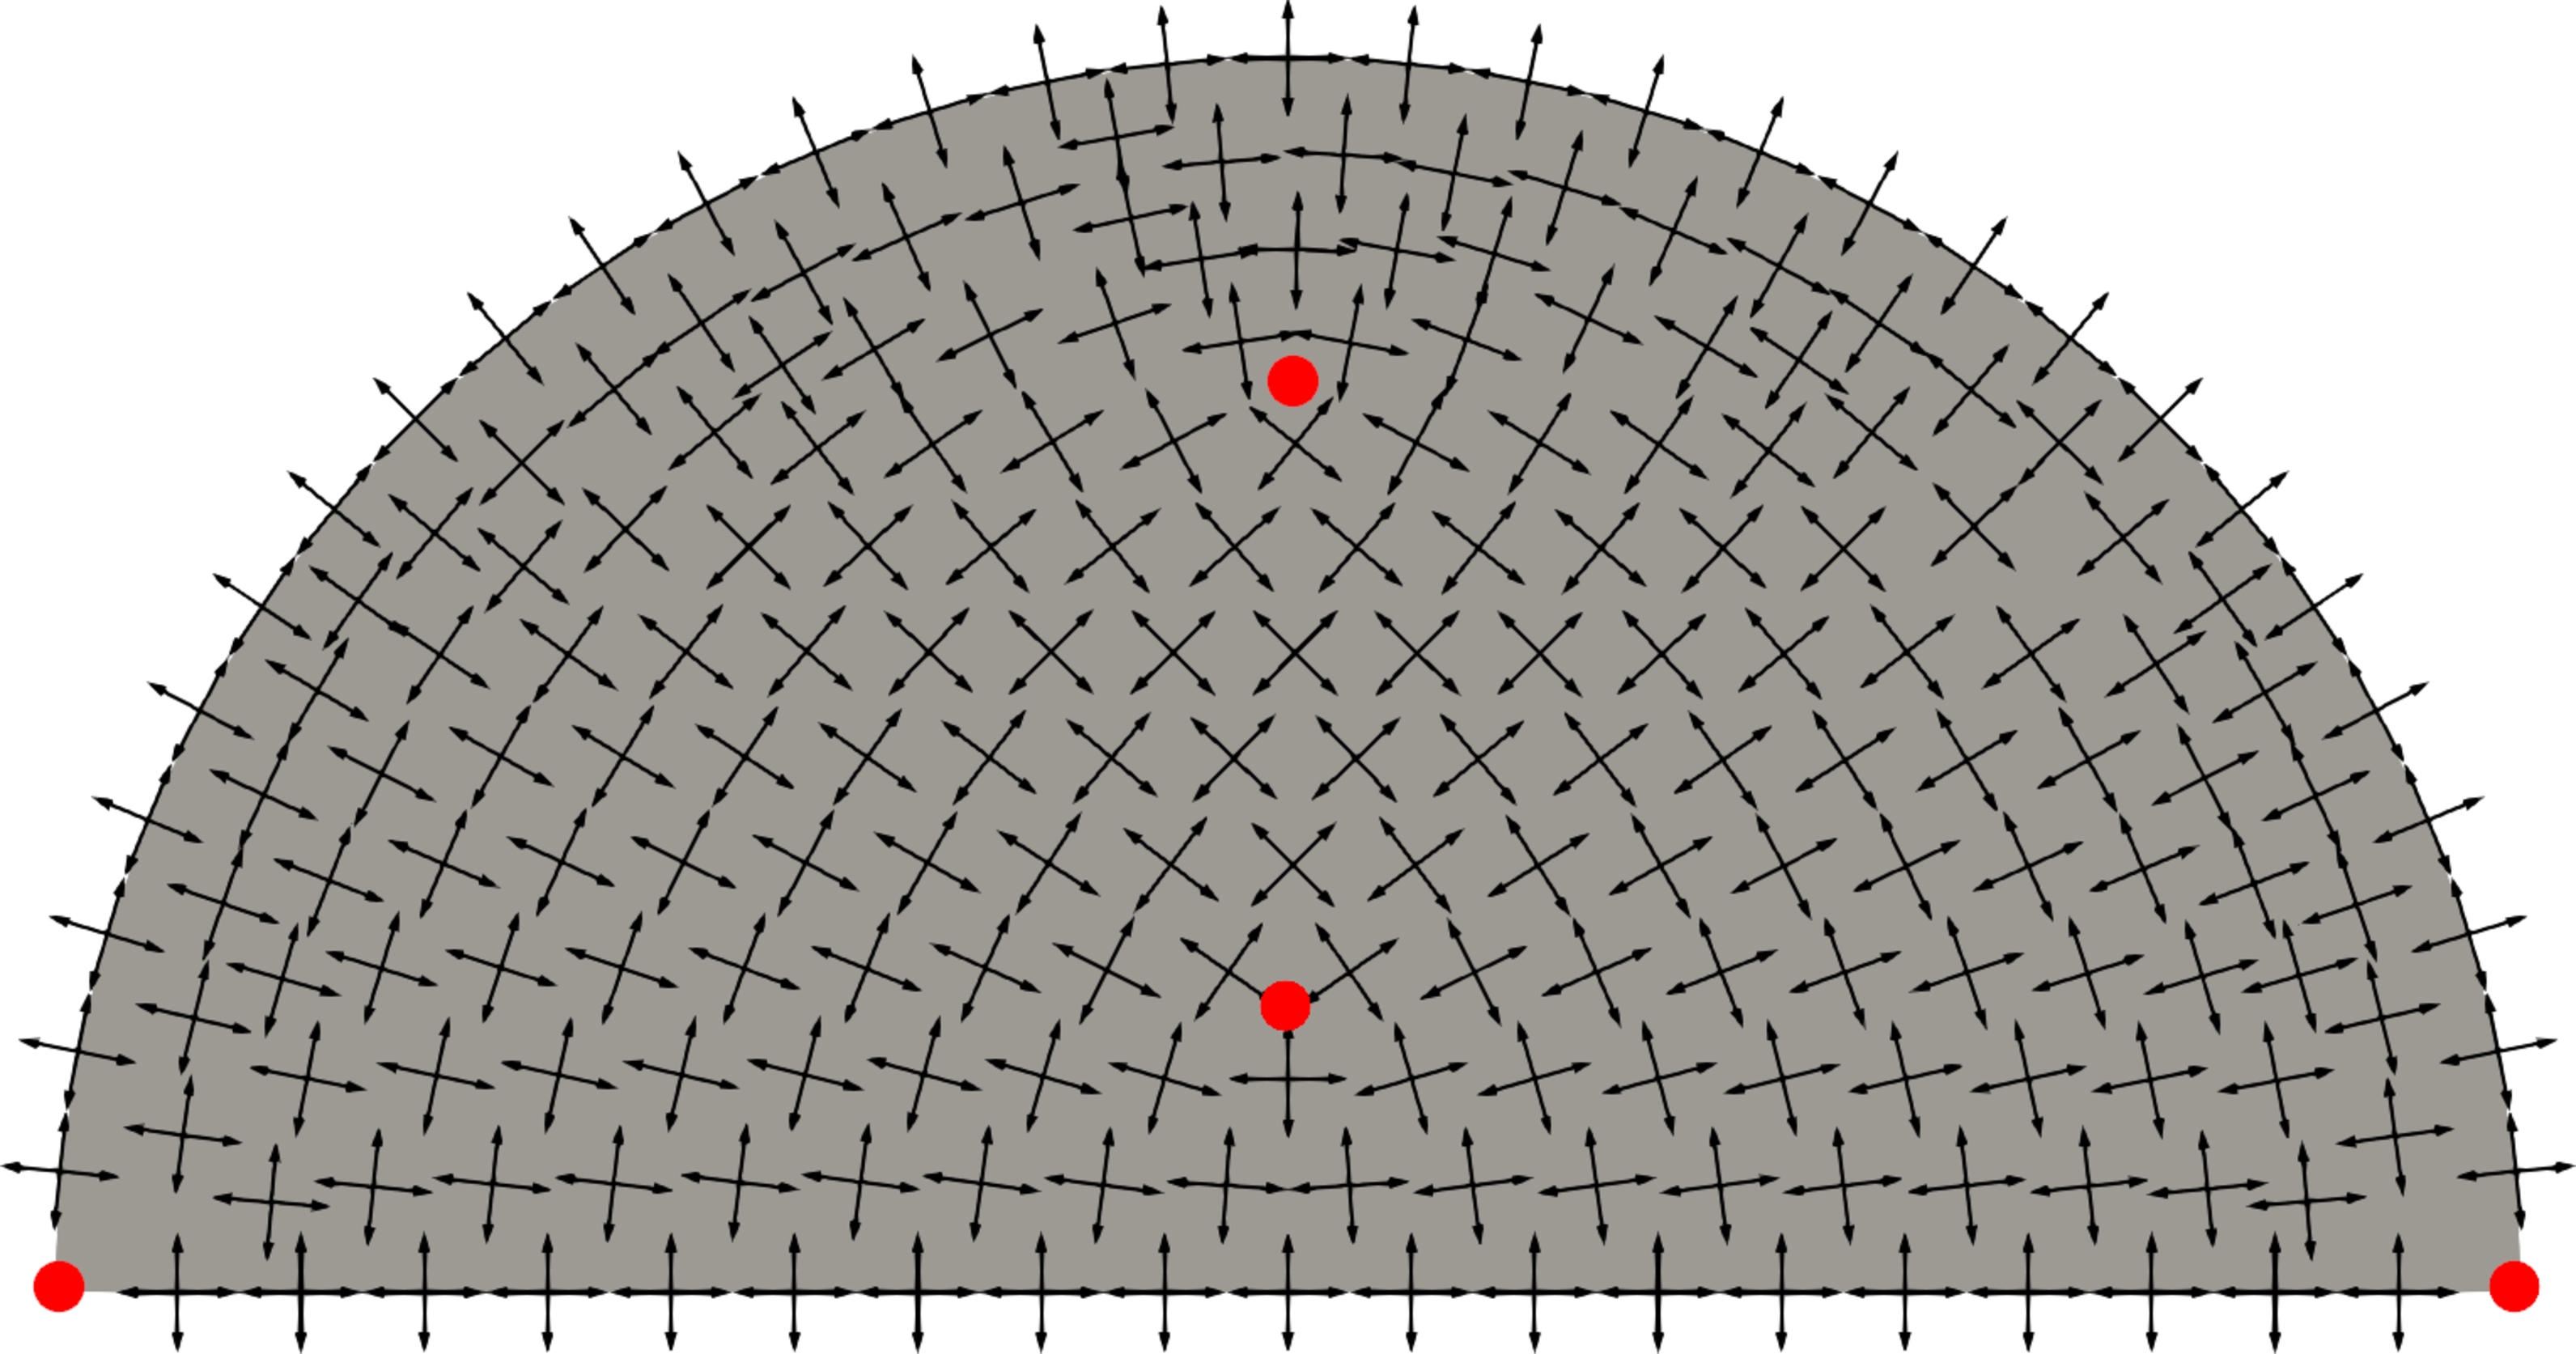
\includegraphics[width=\textwidth]{images/demi_disc_align_first.pdf}
    \caption{Champ de croix aligné sur le bord du domaine (points singuliers en rouge).}
    \label{fig:demi_disc_align_first}
\end{subfigure}
\\[3ex]
\begin{subfigure}{0.64\textwidth}
    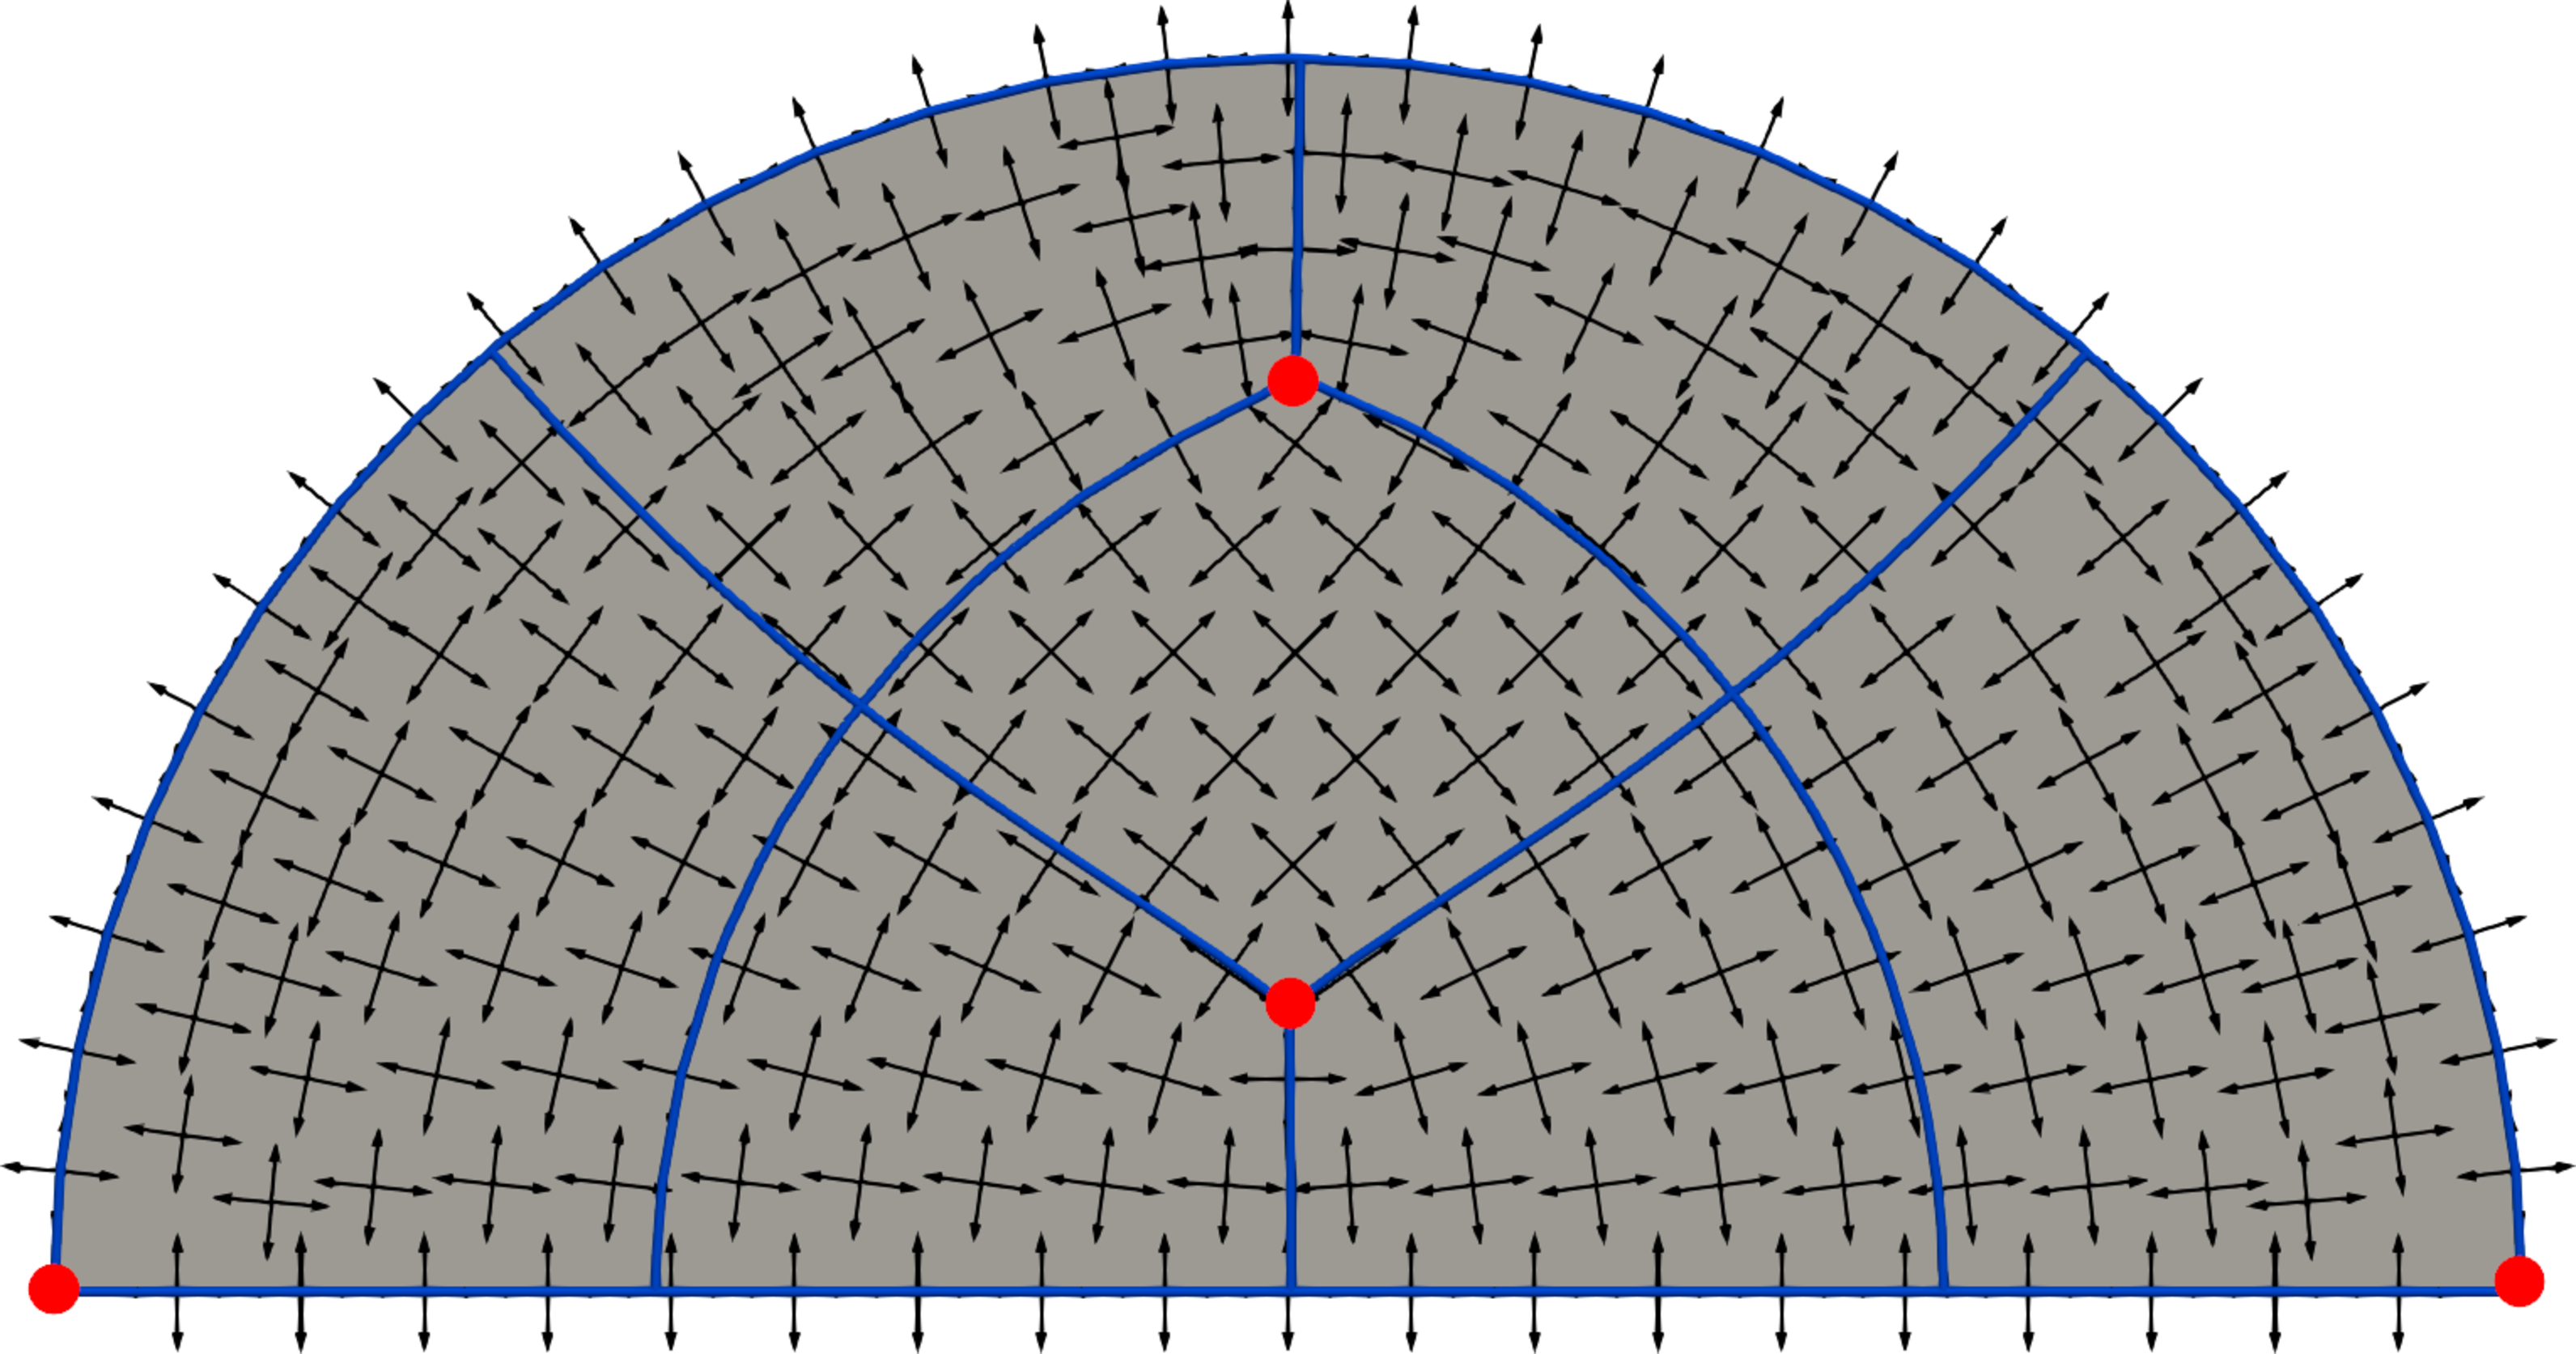
\includegraphics[width=\textwidth]{images/demi_disc_align_second.pdf}
    \caption{Partitionnement du Domaine.}
    \label{fig:demi_disc_align_second}
\end{subfigure}
\\[3ex]
\begin{subfigure}{0.64\textwidth}
    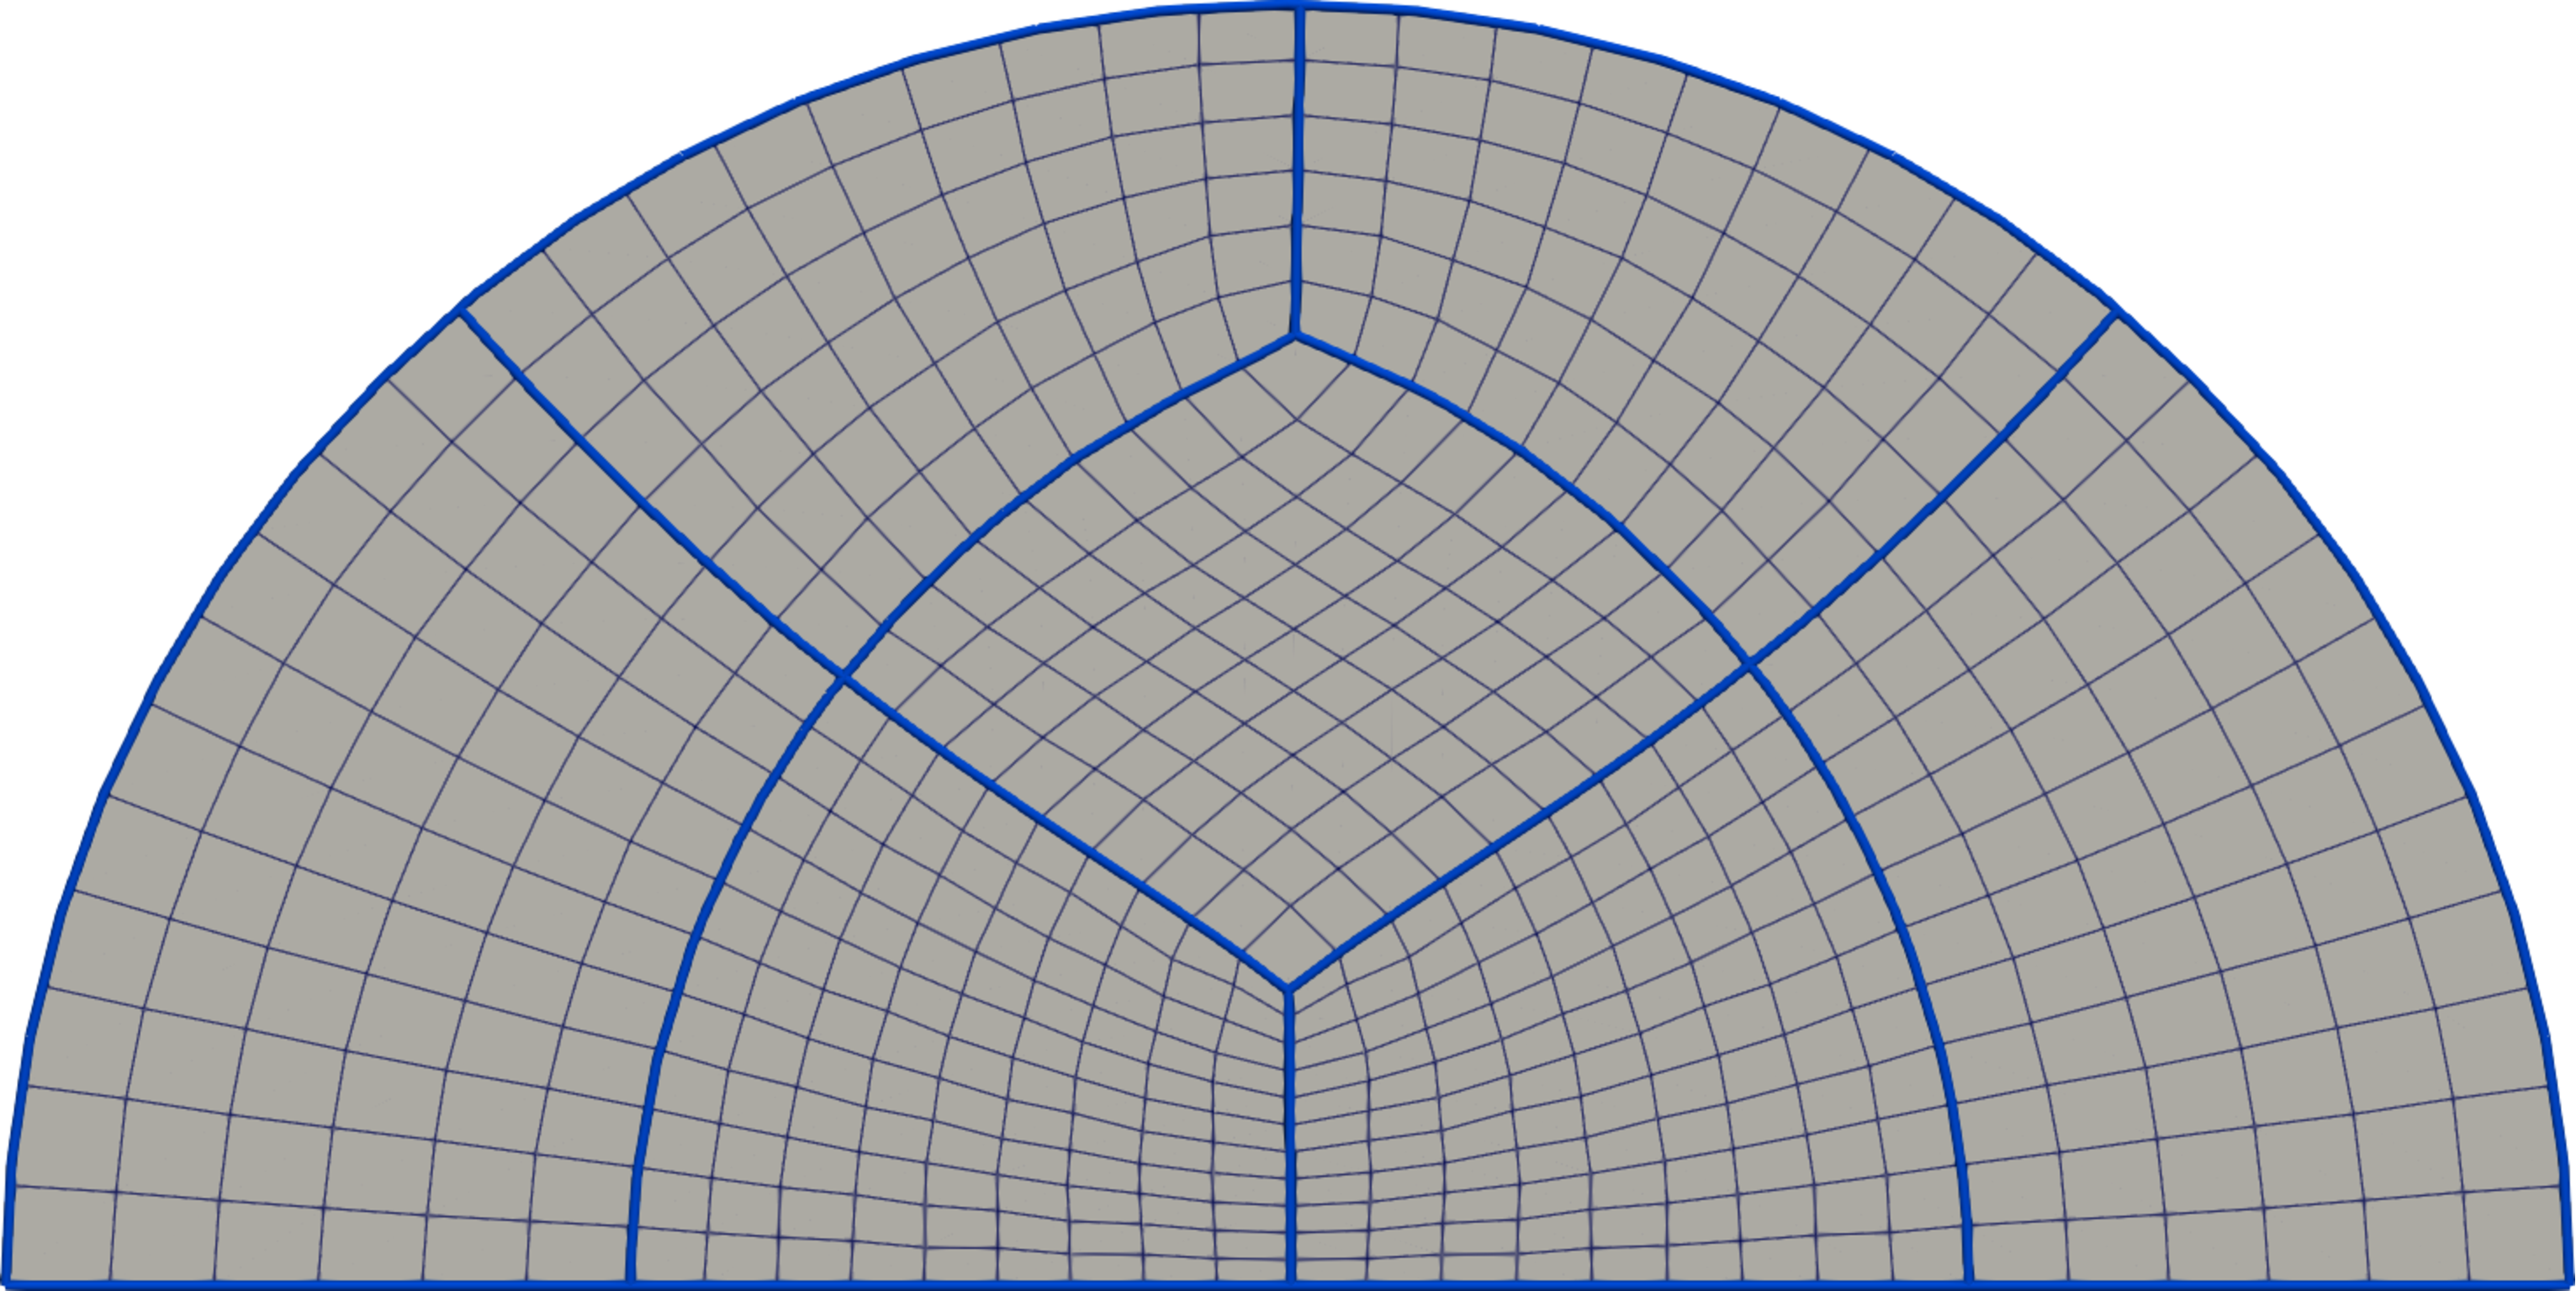
\includegraphics[width=\textwidth]{images/demi_disc_align_third.pdf}
    \caption{Maillage quadilatéral du domaine.}
    \label{fig:demi_disc_align_third}
\end{subfigure}

\caption{Maillage quadrilatéral d'un domaine à partir d'un champ de croix aligné sur le bord du domaine.}
\label{fig:demi_disc_align}
\end{figure}

\subsubsection*{Construction à partir d'un champ de croix non-aligné sur le bord $\Omega$}

Comme indiqué dans l'introduction, notre objectif est de permettre l'utilisation de différents types de champs de croix. Par exemple, un champ de croix peut être construit en prenant le quart de l'angle des vecteurs du champ de gradient d'un mode propre particulier du Laplacien (voir la figure \ref{fig:demiDisc_valProp}). La même construction peut être appliquée aux lignes de niveau.

\begin{figure}[!h]
\centering
\begin{subfigure}{0.65\textwidth}
    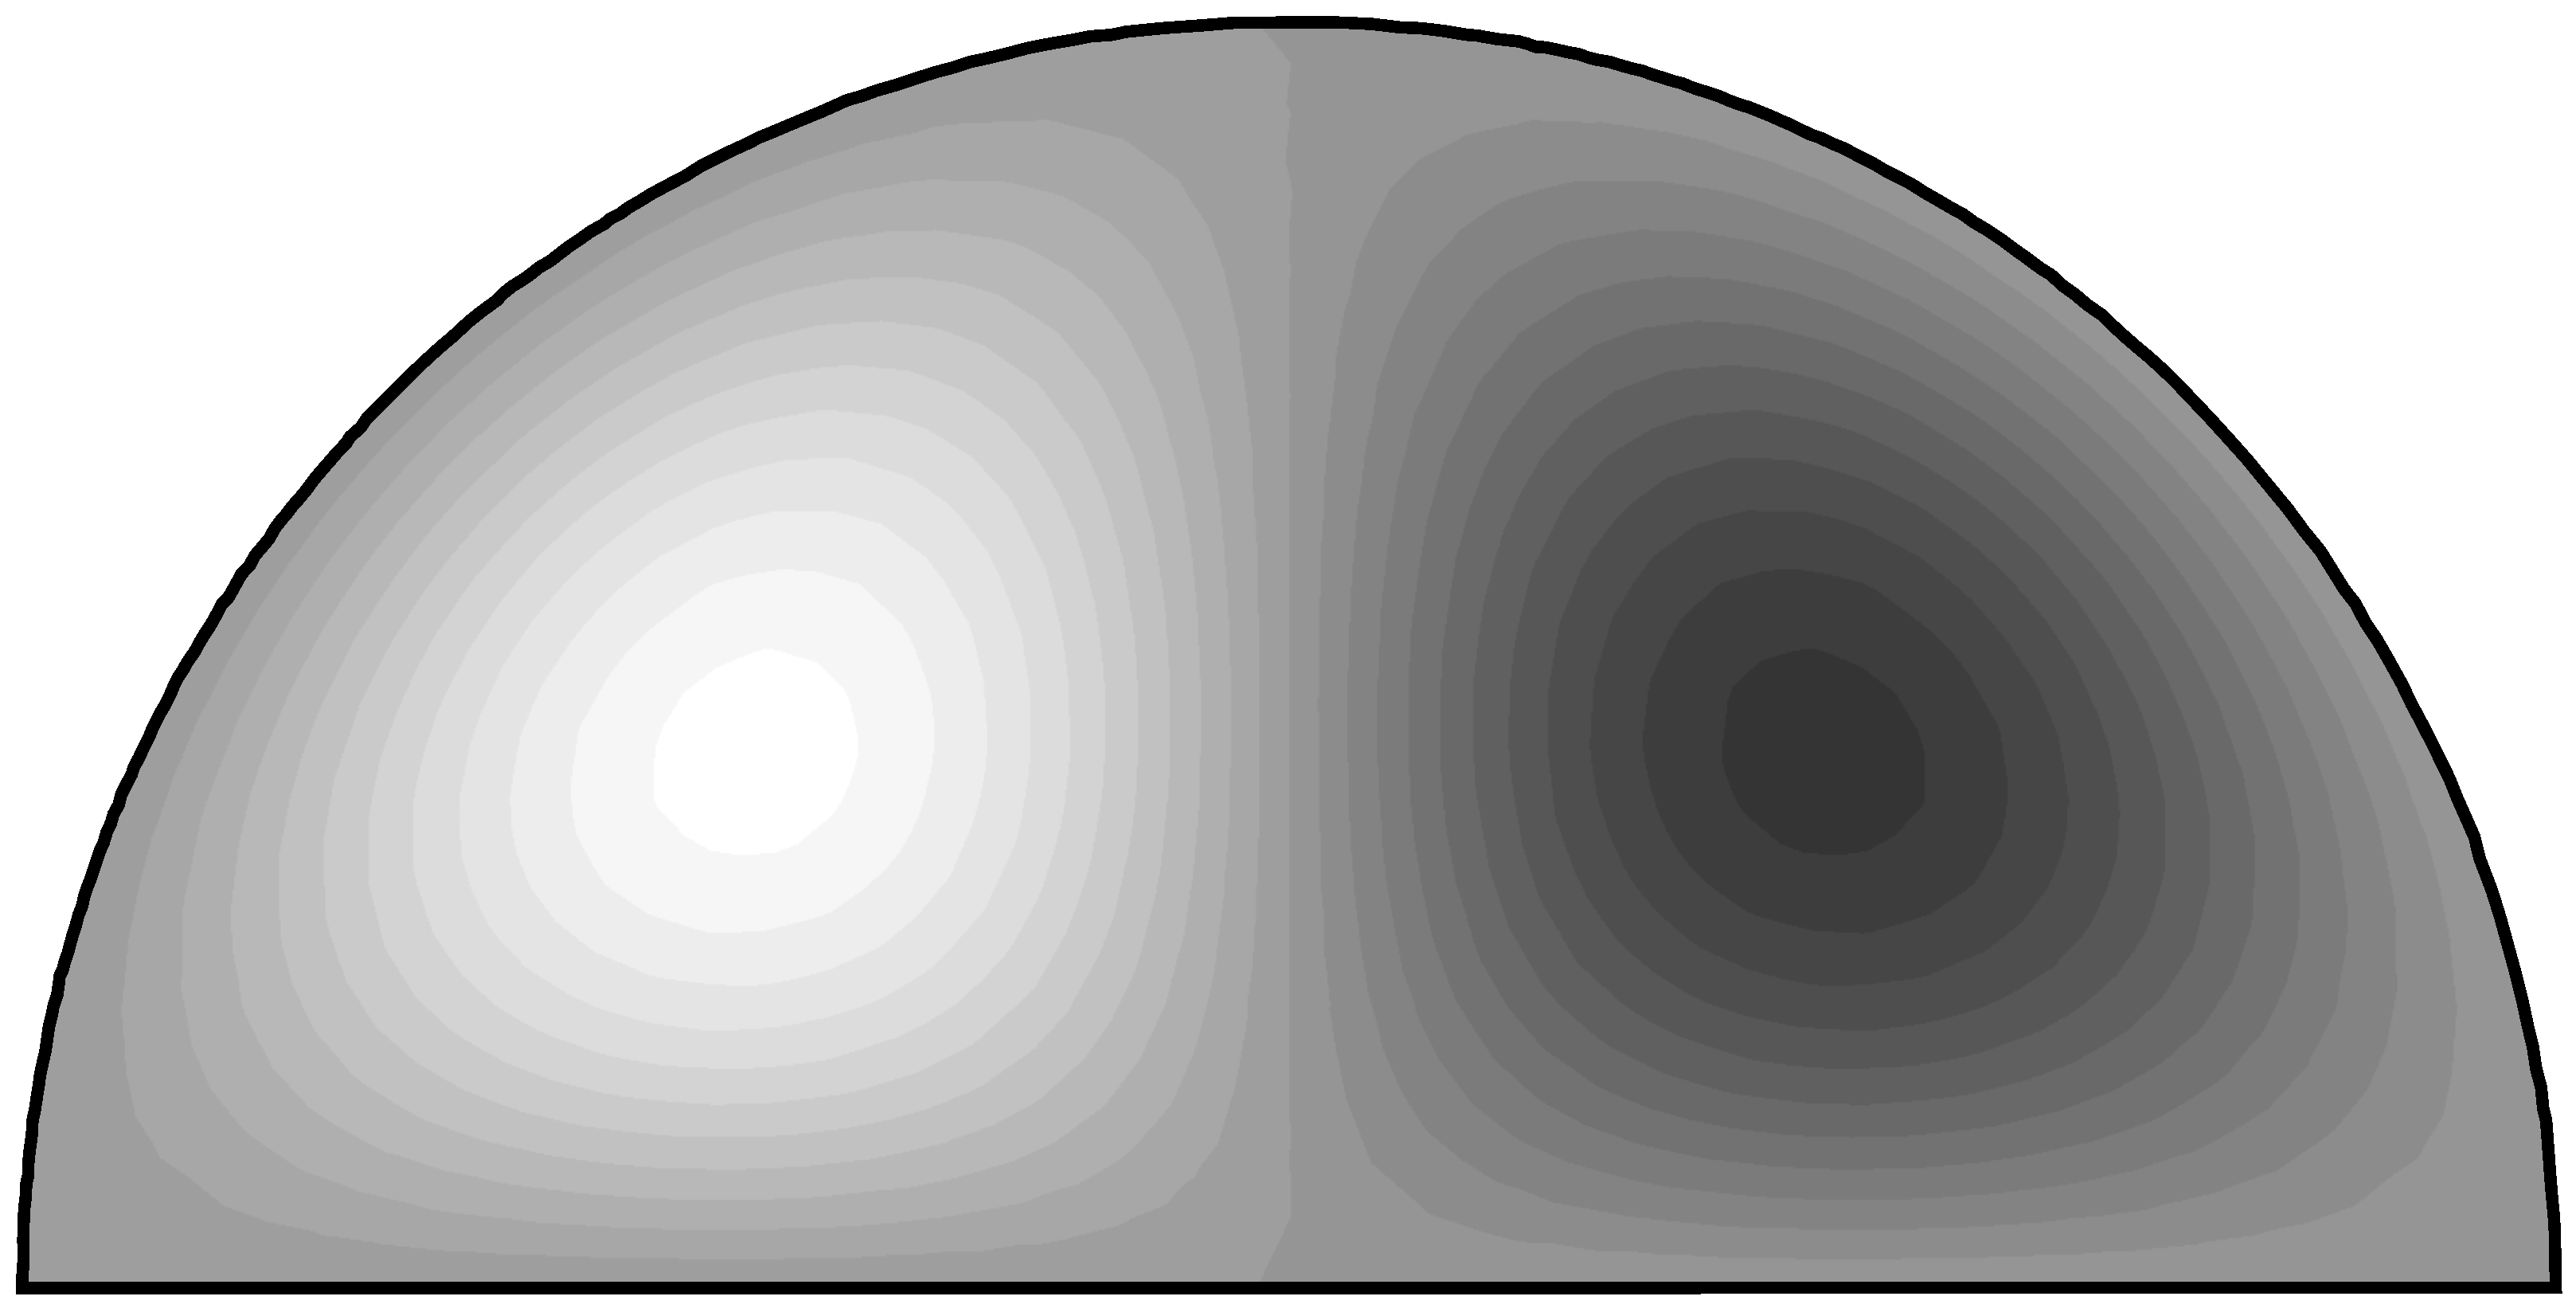
\includegraphics[width=\textwidth]{images/demiDiscValProp.eps}
    \caption{Un mode propre du Laplacien sur le demi disque.}
    \label{fig:demiDiscValPropSheet_first}
\end{subfigure}
\\[3ex]
\begin{subfigure}{0.75\textwidth}
    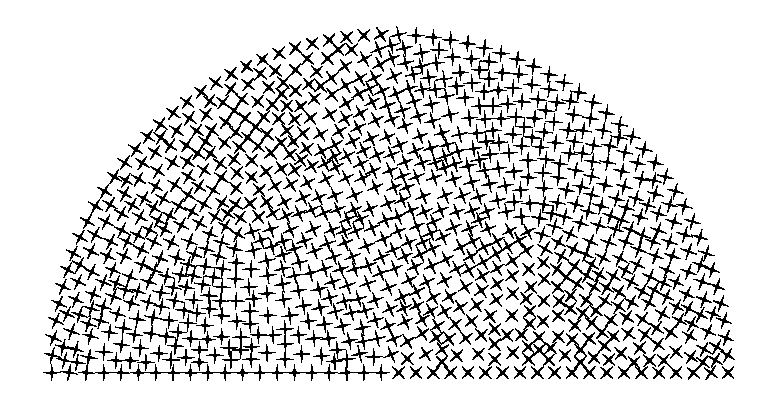
\includegraphics[width=\textwidth]{images/demiDiscValPropSheet.eps}
    \caption{Champ de croix construit à partir du mode propre.}
    \label{fig:demiDiscValPropSheet_second}
\end{subfigure}

\caption{Génération d'un champ de croix à partir d'un mode propre du Laplacien.}
\label{fig:demiDisc_valProp}
\end{figure}

On observe que les extrémas du mode propre coïncident avec les points singuliers correspondants du champ de croix construit. Ces points singuliers sont donc approximativement à une distance égale les uns des autres et de la frontière. Nous visons à conserver cette caractéristique du champ de croix dans le maillage final, ce qui aboutira à une distribution plus uniforme des éléments du maillage. Plus généralement, notre motivation est de choisir d'autres types de champs de croix de manière à ce que le maillage quadrilatéral résultant hérite de certaines propriétés du champ de croix initialement choisi, notamment la position et la nature des points singuliers.

Cependant, lorsqu'un champ de croix, tel que décrit ci-dessus, est utilisé pour diviser le domaine (via l'Algorithme \ref{alg:algo_main}), on constate que certaines régions s'éloignent de la forme quadrilatérale habituelle, comme illustré dans la figure \ref{fig:demiDisc_valProp_mauvaix_decoup}. Cette déviation est due au fait que le champ de croix n'est pas aligné correctement avec les frontières du domaine. Par conséquent, certaines partitions ne possèdent pas quatre côtés.

\begin{figure}[!h]
\centering
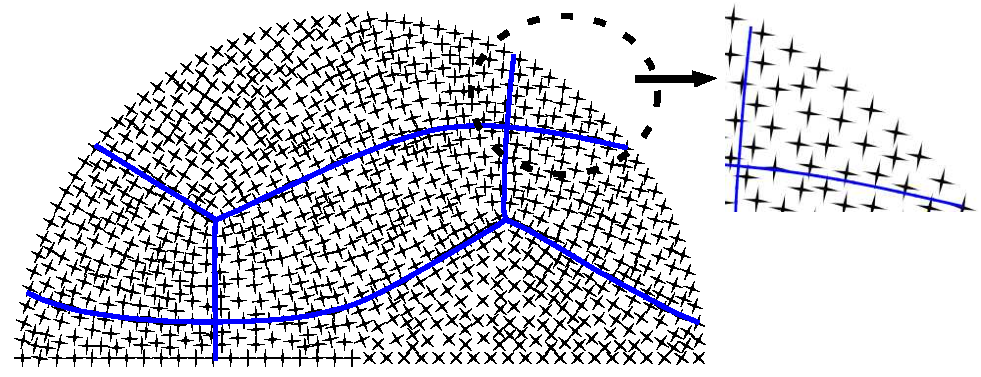
\includegraphics[scale=0.8]{images/gagaga.pdf}
\caption{Découpage invalide obtenue à partir du champ de croix de la figure \ref{fig:demiDisc_valProp}.}
\label{fig:demiDisc_valProp_mauvaix_decoup}
\end{figure}


Pour remédier à cette difficulté, nous introduisons une opération sur le champ de croix appelée \emph{opération d'alignement}. L'objectif est d'ajuster le champ de croix pour qu'il soit aligné avec la frontière du domaine. Pour ce faire, nous cherchons un champ scalaire avec une certaine régularité tel que la rotation du champ de croix initial par rapport à ce champ scalaire donne un nouveau champ de croix aligné avec les frontières du domaine tout en préservant certaines propriétés du champ de croix initial. Dans la suite, nous détaillerons cette opération tout en désignant par \emph{champ d'alignement} le champ scalaire décrit ci-dessus. Pour simplifier la présentation, nous mettons en place l'opération d'alignement dans un premier temps sur un domaine simplement connexe avant de l'étendre aux domaines non-simplement connexes.

\paragraph{Domaine simplement connexe:}
On suppose $\Omega$ simplement connexe. Soit $\bar{u}$ un champ de croix presque-$\mathcal{C}^1$ défini sur $\Omega$ et non-nécessairement aligné sur le bord de $\Omega$ tel que $0<\#\mathcal{S}_{\bar{u}}<\infty$ et pour tout point $p\in\mathcal{S}_{\bar{u}}\backslash\partial\Omega$, $id_{\bar{u}}(p)=k/4$, avec $k\in\mathbb{Z}$ et $k\leq 1$. A priori, une façon simple de réaliser l'opération d'alignement serait de calculer la différence angulaire entre le champ de croix $\bar{u}$ et le champ de croix normal $\bar{N}$ puis de diffuser continûment cette différence angulaire à l'intérieur du domaine. En faisant cela on construirait un champ scalaire régulier sur tout le domaine tel que la rotation du champ de croix par rapport à ce champ scalaire donnerait un champ de croix aligné sur le bord du domaine et n'affectant pas les points singuliers du champ de croix initial en vertu de la proposition $\ref{prop:cont1}$. Un bon candidat pour la diffusion serait alors l'équation de Laplace donné par:\begin{equation}
\left\{
\begin{array}{lcll}
\Delta\phi &=& 0 &\mbox{ dans }\Omega,\\[0.5cm]
\phi(p) &=& \widehat{(\bar{N}(p); \bar{u}(p))}=\theta_{\bar{N}}(p)-\theta_{\bar{u}}(p)&\mbox{ sur } \partial\Omega,
\end{array}
\right.
\label{eqn:first_phi_computation}
\end{equation}
où $\widehat{(\bar{N}(p); \bar{u}(p))}$ représente l'angle entre $\bar{N}(p)$ et $\bar{u}(p)$. En définissant $\bar{v}:=\mathbf{R}(\phi)\bar{u}$, il est évident que $\bar{v}=\bar{N}$ sur $\partial\Omega$, impliquant ainsi que $\bar{v}$ est aligné avec $\partial\Omega$. De plus, grâce à la proposition \ref{prop:relation_u_Rthetau}, nous savons que pour tout $p\in\Omega\backslash\partial\Omega$, $id_{\bar{v}}(p)=id_{\bar{u}}(p)$. Par conséquent, si l'algorithme de partitionnement \ref{alg:algo_main} converge lorsqu'il est appliqué à $\bar{v}$, nous obtenons un partitionnement de $\Omega$ en régions à quatre côtés (voir le Théorème \ref{thm:theorem1}). Cependant, une question demeure en suspens : quelle est la valeur des indices des points situés sur le bord de $\Omega$ dans le champ de croix $\bar{v}$? Cela va dépendre de la représentation angulaire choisie pour $\phi$ à un multiple de $\pi/2$ près dans la condition de bord de l'équation \eqref{eqn:first_phi_computation}.

\begin{figure}[!h]
\centering
\begin{subfigure}{0.65\textwidth}
    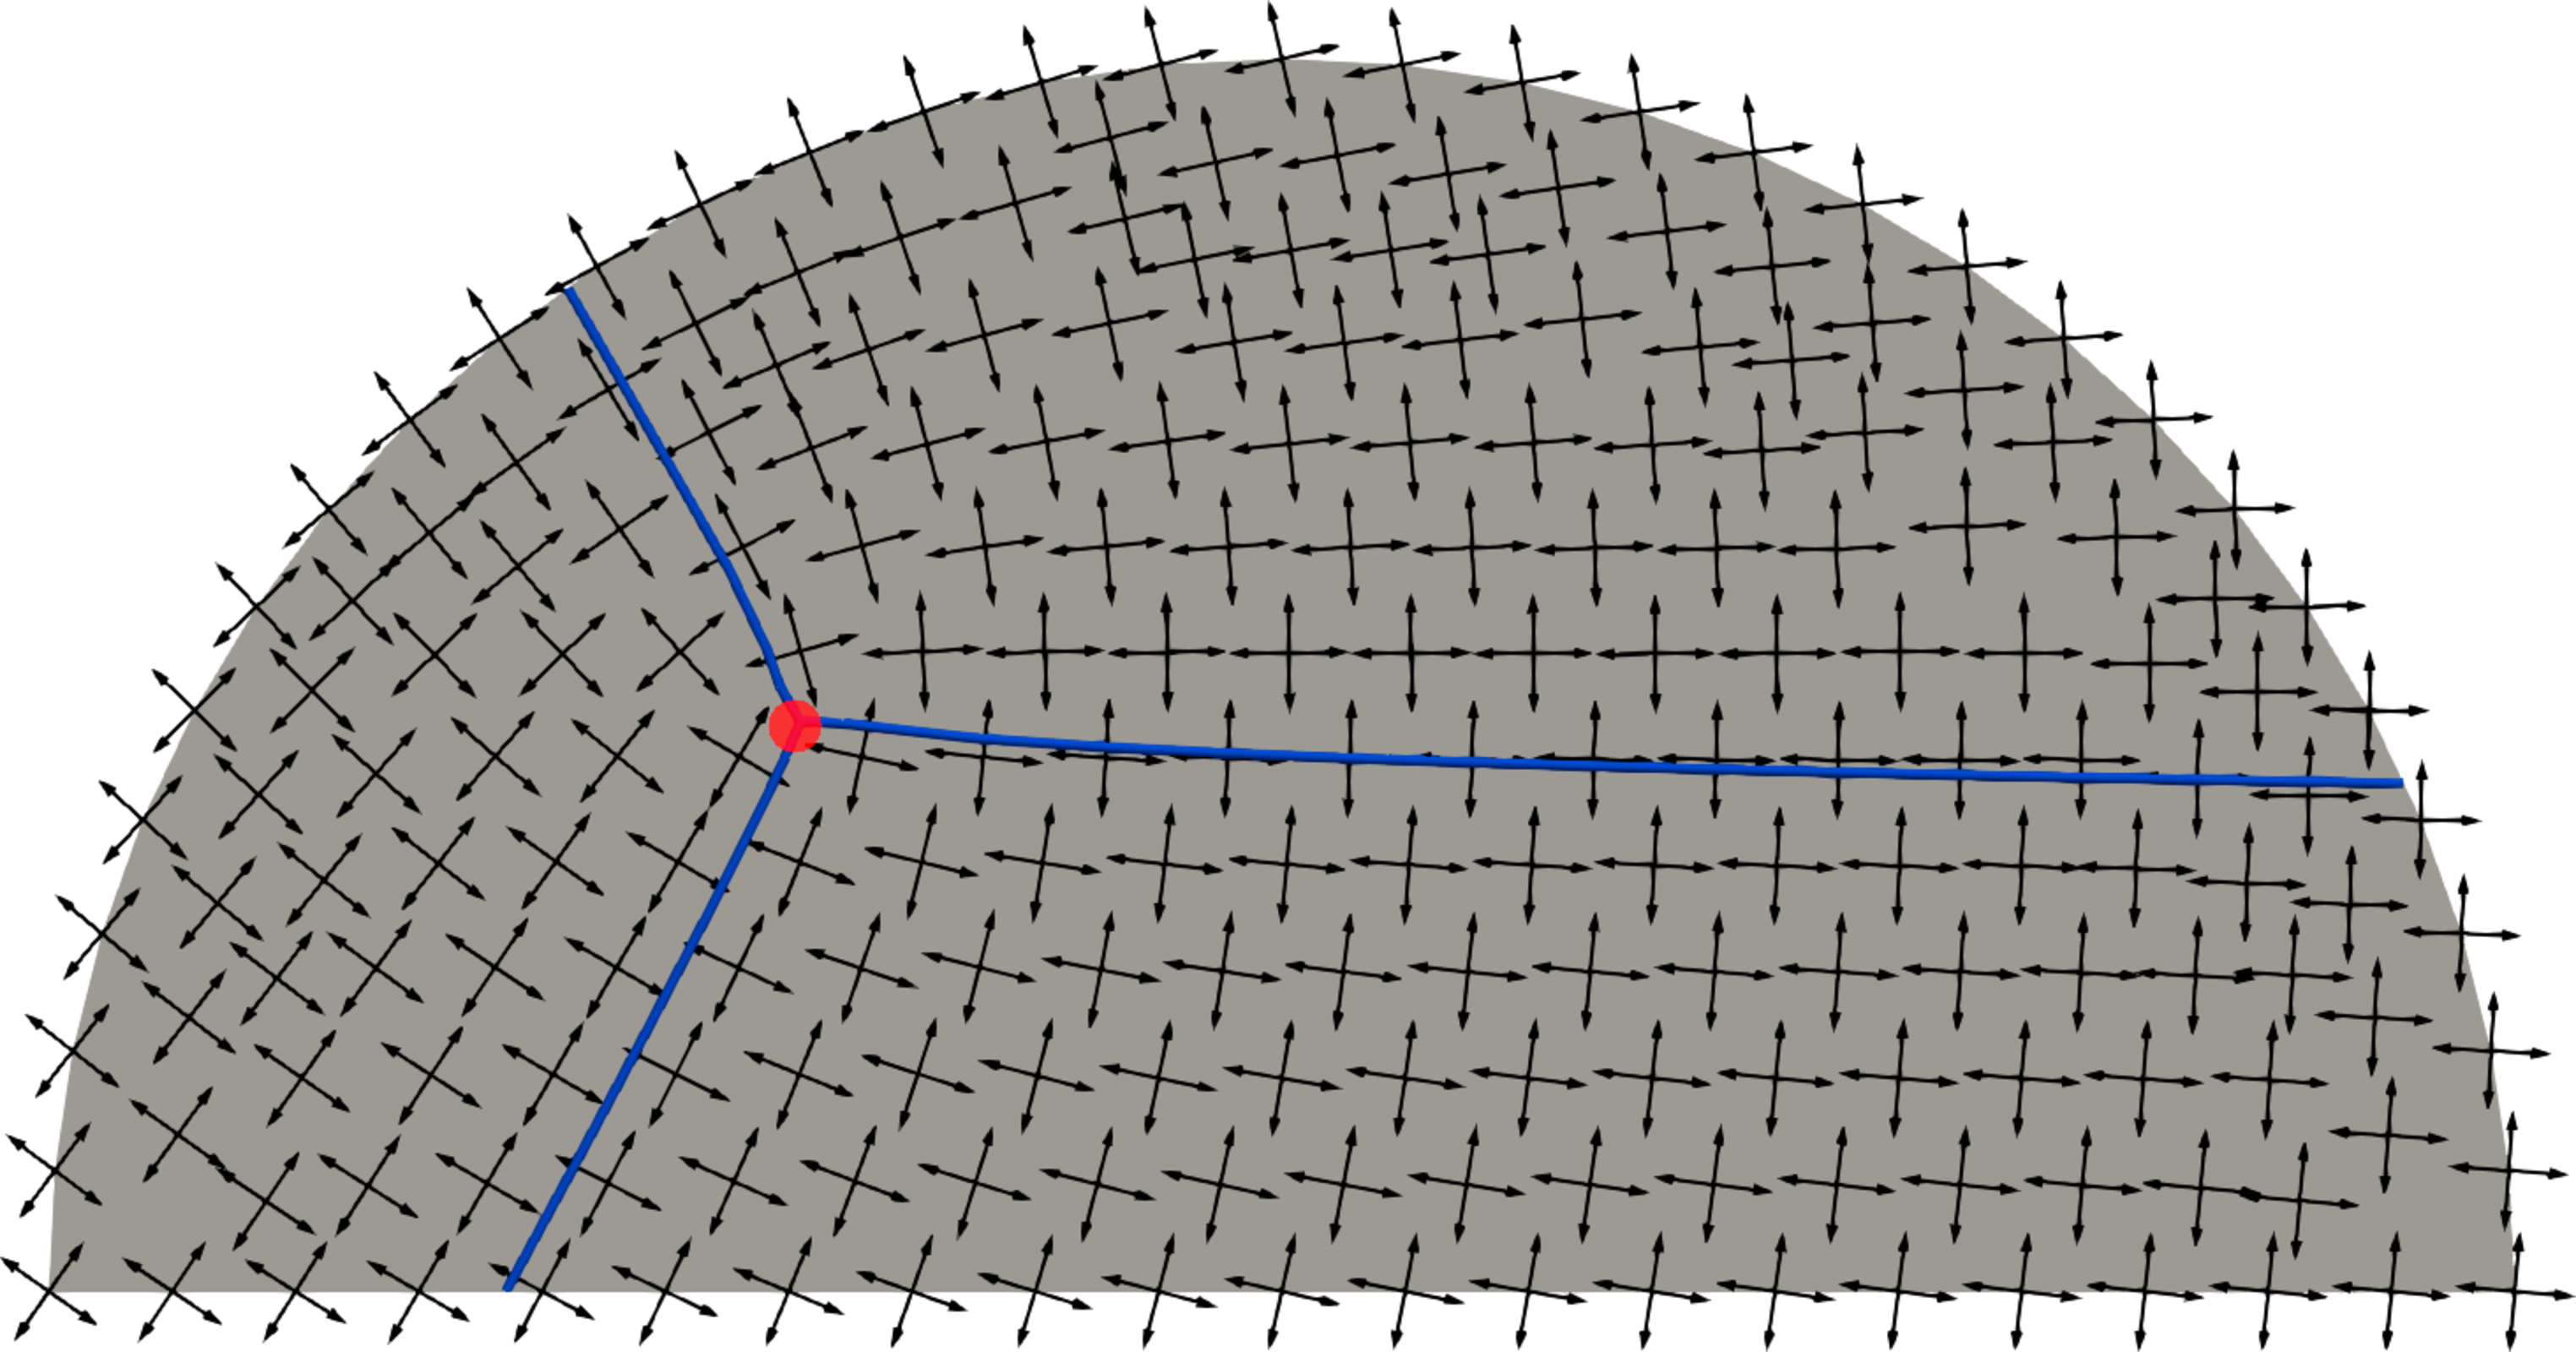
\includegraphics[width=\textwidth]{images/demi_disc_first_phi_first.pdf}
    \caption{Champ de croix initial avec un point singulier interne d'indice $1/4$.}
    \label{fig:demi_disc_first_cond_phi_first}
\end{subfigure}
\\[0.4cm]
\begin{subfigure}{0.65\textwidth}
    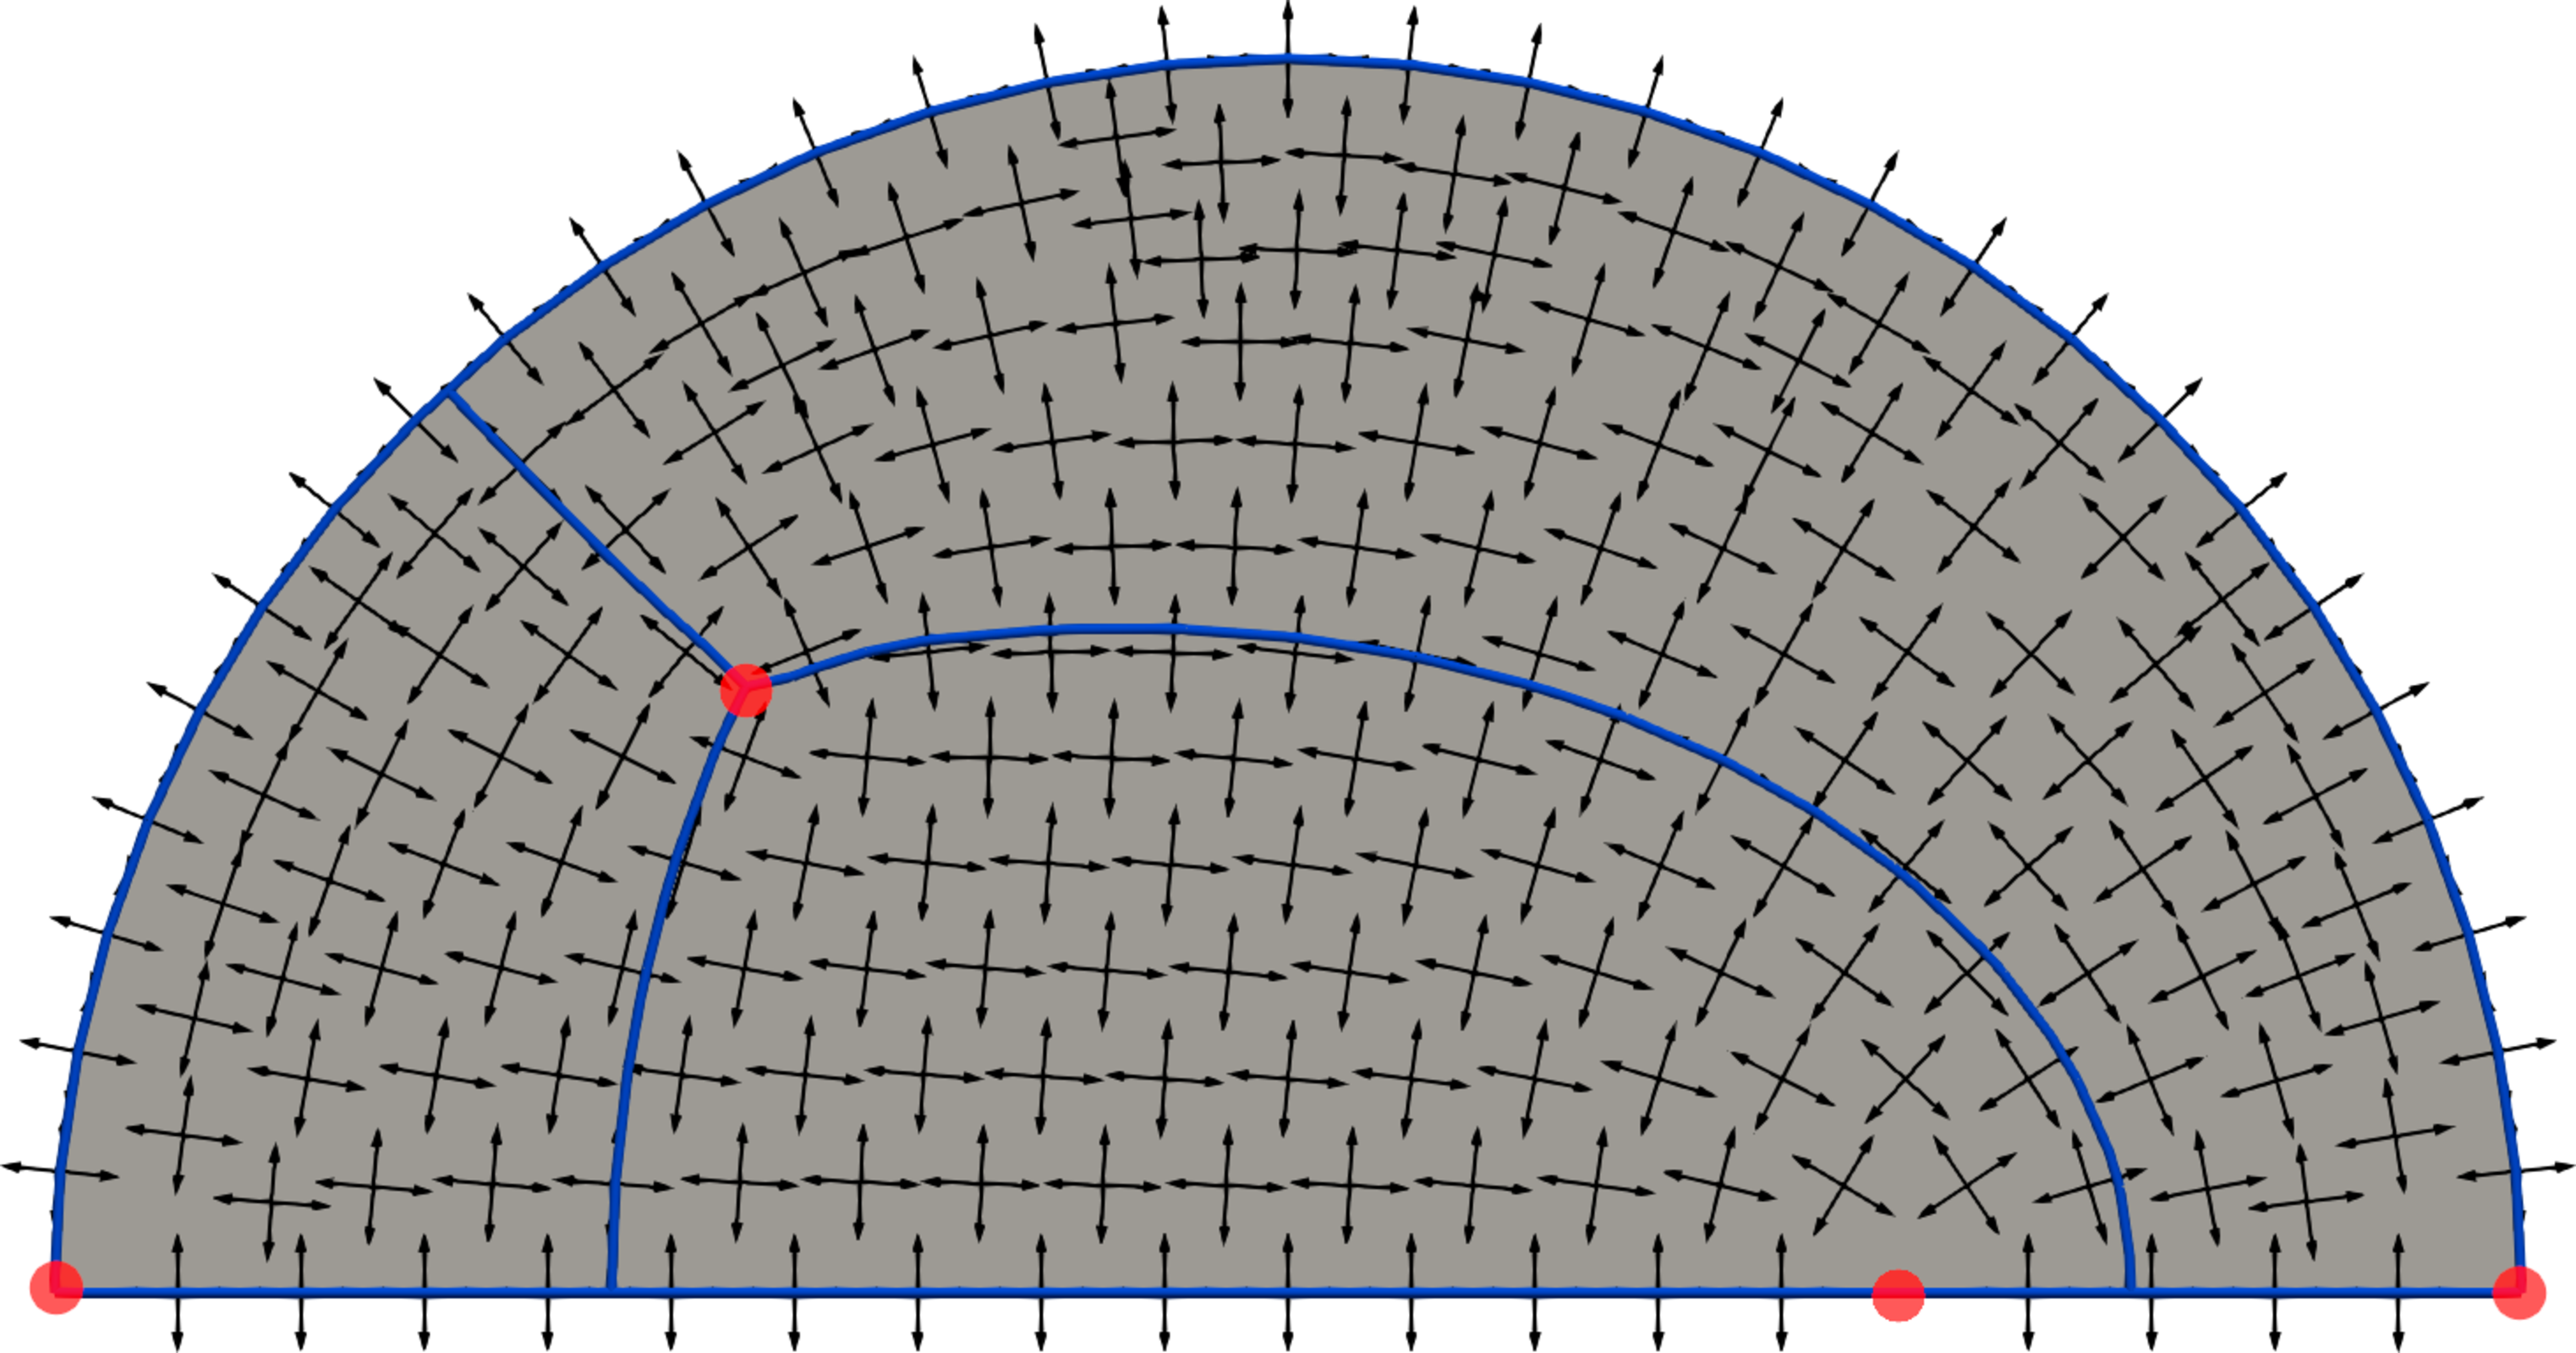
\includegraphics[width=\textwidth]{images/demi_disc_first_phi_second.pdf}
    \caption{Alignement du champ de croix initial sur le bord du domaine et partitionnement du domaine.}
    \label{fig:demi_disc_first_cond_phi_second}
\end{subfigure}
\\[0.4cm]
\begin{subfigure}{0.65\textwidth}
    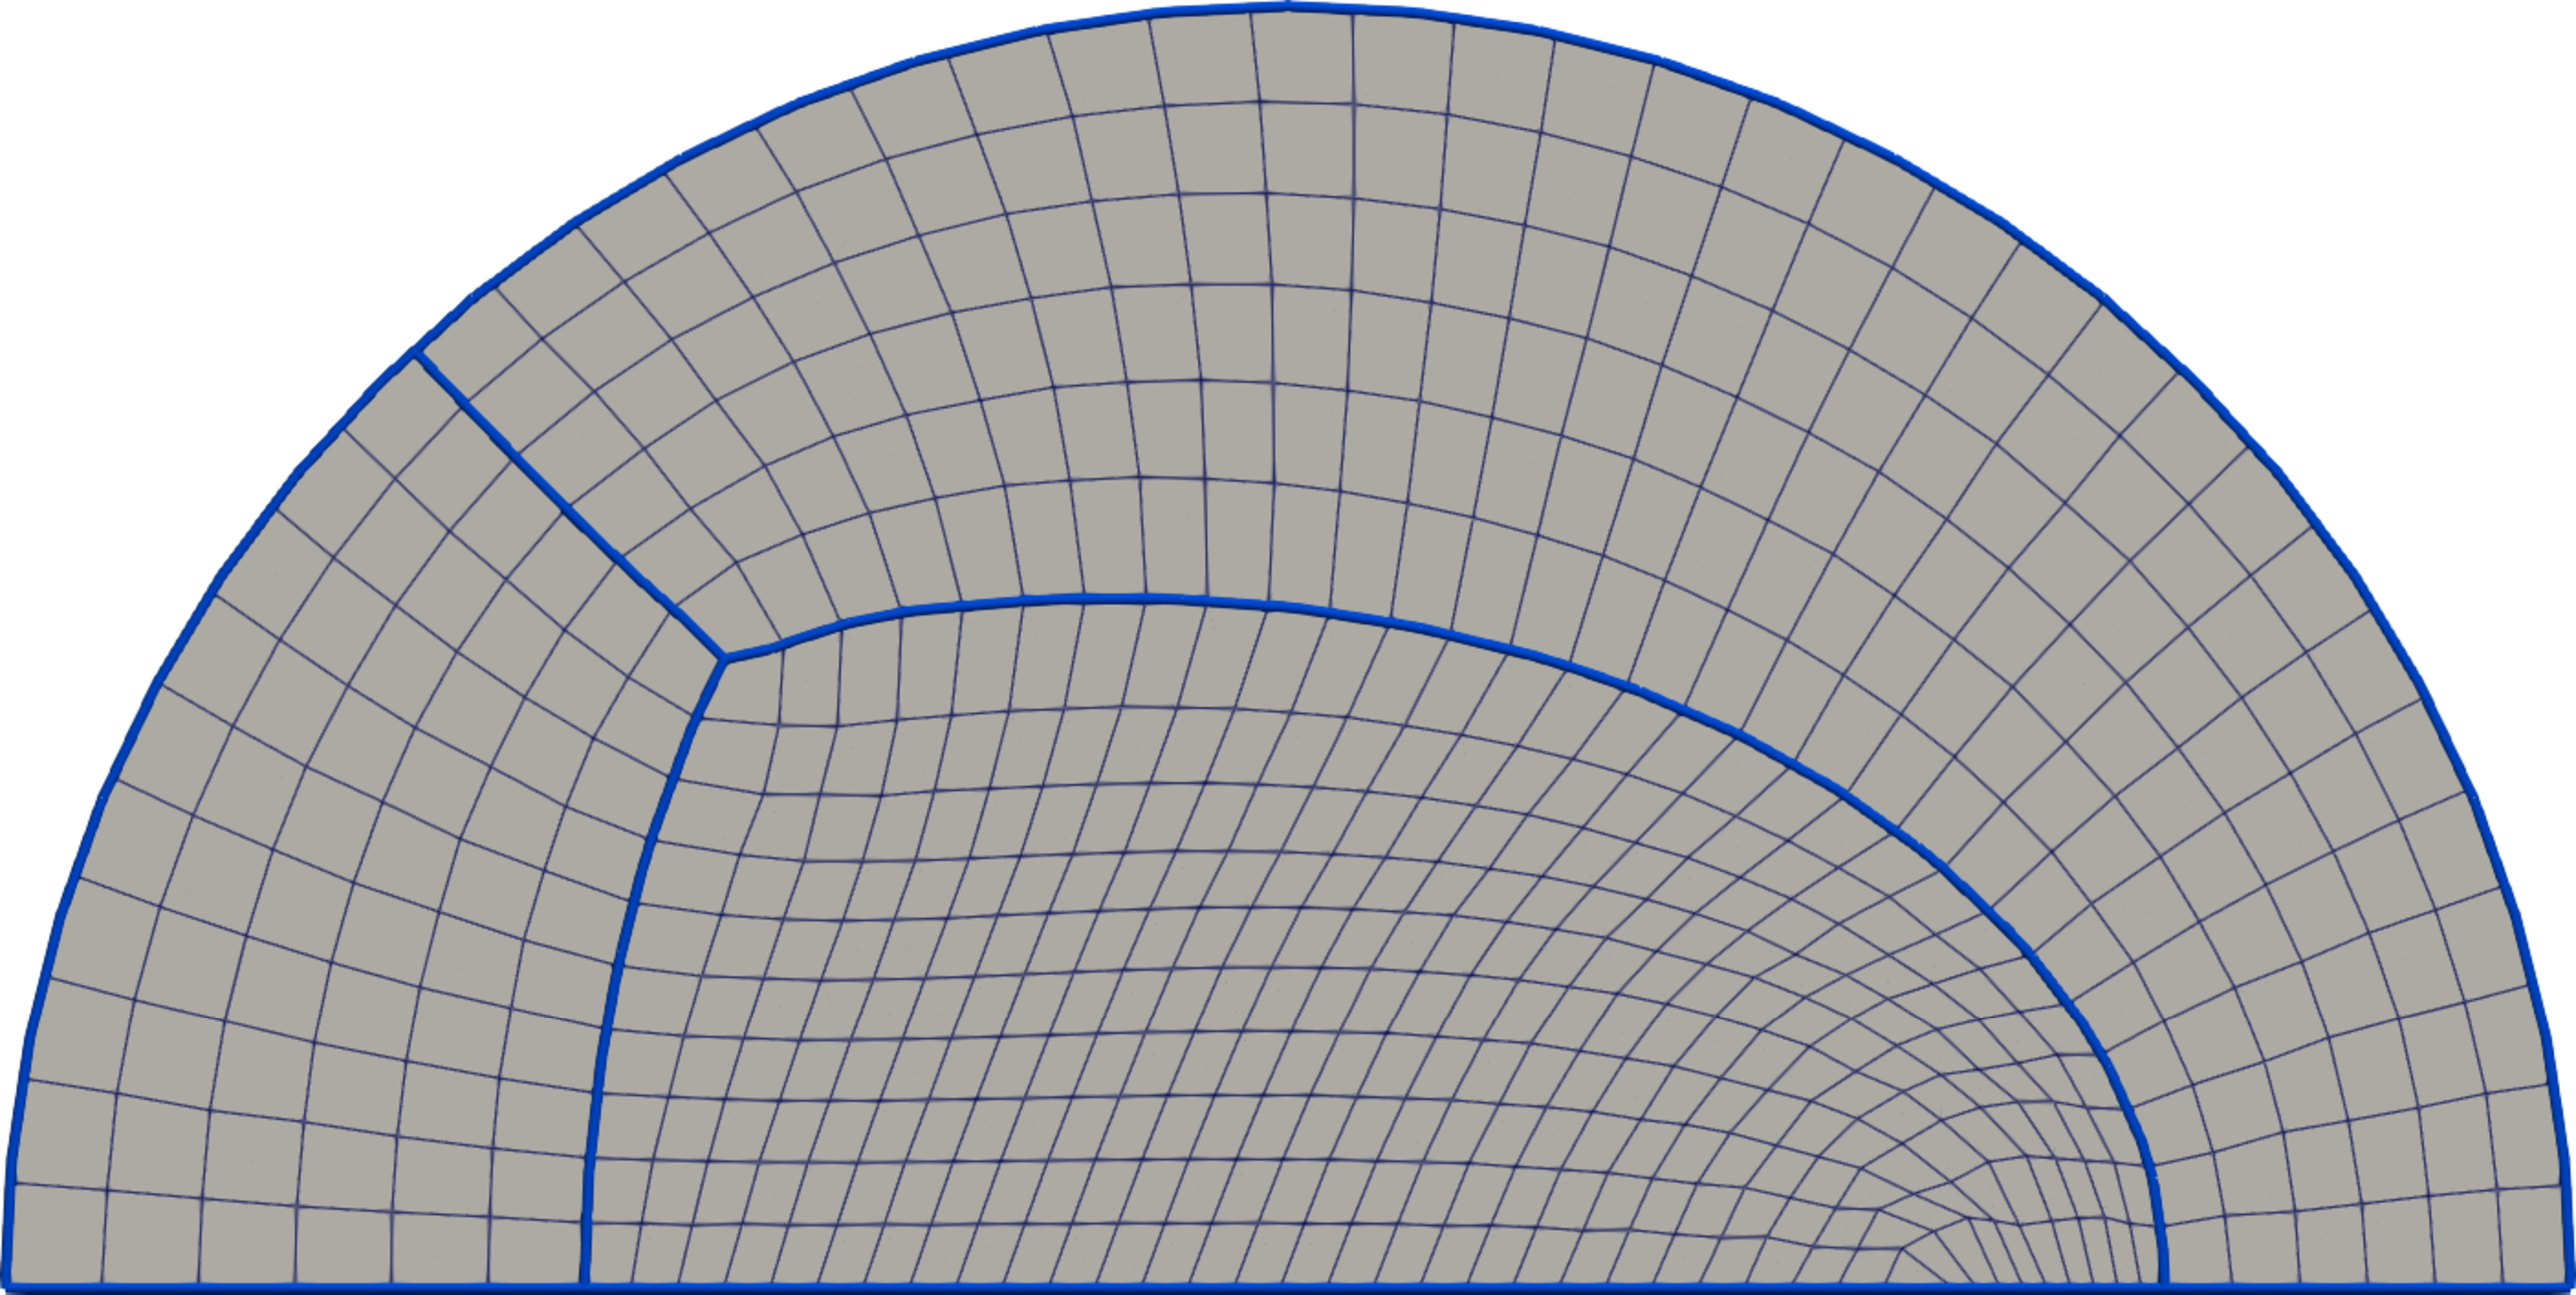
\includegraphics[width=\textwidth]{images/demi_disc_first_phi_third.pdf}
    \caption{Maillage quadilatéral du domaine présentant un quadrangle dégénéré.}
    \label{fig:demi_disc_first_cond_phi_third}
\end{subfigure}

\caption{Illustration de l'opération d'alignement à partir du champ d'angle donné par l'équation \eqref{eqn:first_phi_computation}.}
\label{fig:demi_disc_first_cond_phi}
\end{figure}

En l'état, nous n'avons donc aucun contrôle sur la régularité de cette condition de bord, ce qui entraînera des effets indésirables dans le maillage quadrilatéral construit à partir du partitionnement obtenu. Par exemple, sur la figure \ref{fig:demi_disc_first_cond_phi}, nous considérons un champ de croix initial possédant une singularité d'indice $1/4$ à l'intérieur du domaine (figure \ref{fig:demi_disc_first_cond_phi_first}). Le champ d'alignement est calculé avec l'équation \eqref{eqn:first_phi_computation}, puis le champ de croix $\bar{v}$ est construit. On observe clairement que $\bar{v}$ est bien aligné avec le bord du domaine et conserve la singularité interne du champ de croix initial. Cependant, on remarque l'apparition de singularités de bord dans le champ de croix $\bar{v}$. En appliquant l'algorithme de partitionnement \ref{alg:algo_main} sur $\bar{v}$, le partitionnement obtenu présente des régions à quatre côtés (figure \ref{fig:demi_disc_first_cond_phi_second}) mais, la présence de points singuliers de bord non contrôlés (en termes de positionnement et d'indice) conduit à un maillage quadrilatéral comportant des quadrangles dégénérés (figure \ref{fig:demi_disc_first_cond_phi_third}).


Afin de remédier à cette situation, nous allons modifier le processus d'alignement en ajustant la condition de Dirichlet de l'équation \eqref{eqn:first_phi_computation} et en imposant des conditions sur le champ de croix initial $\bar{u}$.

Pour commencer, nous définissons l'ensemble des points $\partial\Omega$ qui seront les points singuliers du champ de croix final (issu de l'opération d'alignement). Soit $\mathcal{B}$ cet ensemble. À chaque point $p\in\partial\Omega$, nous associons ensuite un paramètre $I_p$ qui satisfait:

\begin{equation}
I_p=
\left\{
\begin{array}{ll}
    \displaystyle\frac{k}{4}\mbox{ avec }k\in\mathbb{Z}\mbox{ et }k\leq 1&\mbox{ si }p\in\mathcal{B},\\[0.5cm]
    0&\mbox{ sinon}.
\end{array}
\right.
\label{eqn:hyp_I_p}
\end{equation}

Un critère a priori pour le choix automatique de ce paramètre sera exposé ultérieurement dans la section \ref{sec:discussion}. Soit $\gamma$, une paramétrisation sur $[0, 1]$ de $\partial\Omega$ dans le sens positif et vérifiant $\gamma(0)=\gamma(1)\notin\mathcal{S}_{\bar{u}}\cup\mathcal{B}$. Nous imposons ensuite la condition suivante sur le champ de croix $\bar{u}$: il existe $\theta_{\bar{u}}^\gamma$ un relèvement continu de $\bar{u}$ le long de $\gamma$ tel que:
\begin{equation}
    \label{eqn:principe_hypothese_u}
    \theta_{\bar{u}}^\gamma(1)-\theta_{\bar{u}}^\gamma(0)=2\pi\chi(\Omega)-2\pi\sum_{p\in\mathcal{B}}I_p.
\end{equation}
L'opération d'alignement est alors formulé de la manière suivante:\\\\
\textbf{Opération d'alignement:} étant donné $\bar{u}$, nous définissons le champ de croix $\bar{v}$ pour tout $p\in\Omega$ par:
\begin{equation}
\bar{v}(p)=
\left\{
\begin{array}{ll}
\mathbf{R}(\phi(p))\bar{u}(p) & \mbox{ si } p\in\Omega\backslash(\mathcal{B}\cup\mathcal{S}_{\bar{u}}),\\[0.5cm]
\bar{N}(p) & \mbox{ si } p\in(\mathcal{S}_{\bar{u}}\cap\partial\Omega)\backslash\mathcal{B},\\[0.5cm]
0 & \mbox{ si } p\in\mathcal{B}.
\end{array}
\right.
\label{eqn:principe_def_v}
\end{equation}
où $\phi:\Omega\longrightarrow\mathbb{R}$ est définie comme la solution de l'équation de Laplace suivante:
\begin{equation}
\left\{
\begin{array}{lcll}
\Delta\phi &=& 0 &\mbox{ dans }\Omega,\\[0.5cm]
\phi(\gamma(t))&=&\theta_{\bar{N}}^\gamma(t)+\mathcal{I}(t)-\theta_{\bar{u}}(\gamma(t))& \mbox{ sur } \gamma^{-1}(\partial\Omega\backslash(\mathcal{B}\cup\mathcal{S}_{\bar{u}})),
\end{array}
\right.
\label{eqn:principe_def_phi}
\end{equation}
où la fonction $\mathcal{I}$ est donnée pour tout $t\in\gamma^{-1}(\partial\Omega\backslash(\mathcal{B}\cup\mathcal{S}_{\bar{u}}))$ par:
$$
\mathcal{I}(t)=\sum_{s\in\gamma^{-1}(\mathcal{B})}\left[\left(\pi-\widehat{\gamma(s)}-2\pi I_{\gamma(s)}\right)-\left(\lim\limits_{r\rightarrow s^+}\theta^{\gamma}_{\bar{N}}(r) - \lim\limits_{r\rightarrow s^-}\theta^{\gamma}_{\bar{N}}(r)\right)\right]\mathbb{1}_{[0, t]}(s),
$$
avec $\widehat{\gamma(s)}$ la mesure de l'ouverture angulaire de la frontière en $\gamma(s)$.

\begin{figure}[!h]
\centering
\begin{subfigure}{0.65\textwidth}
    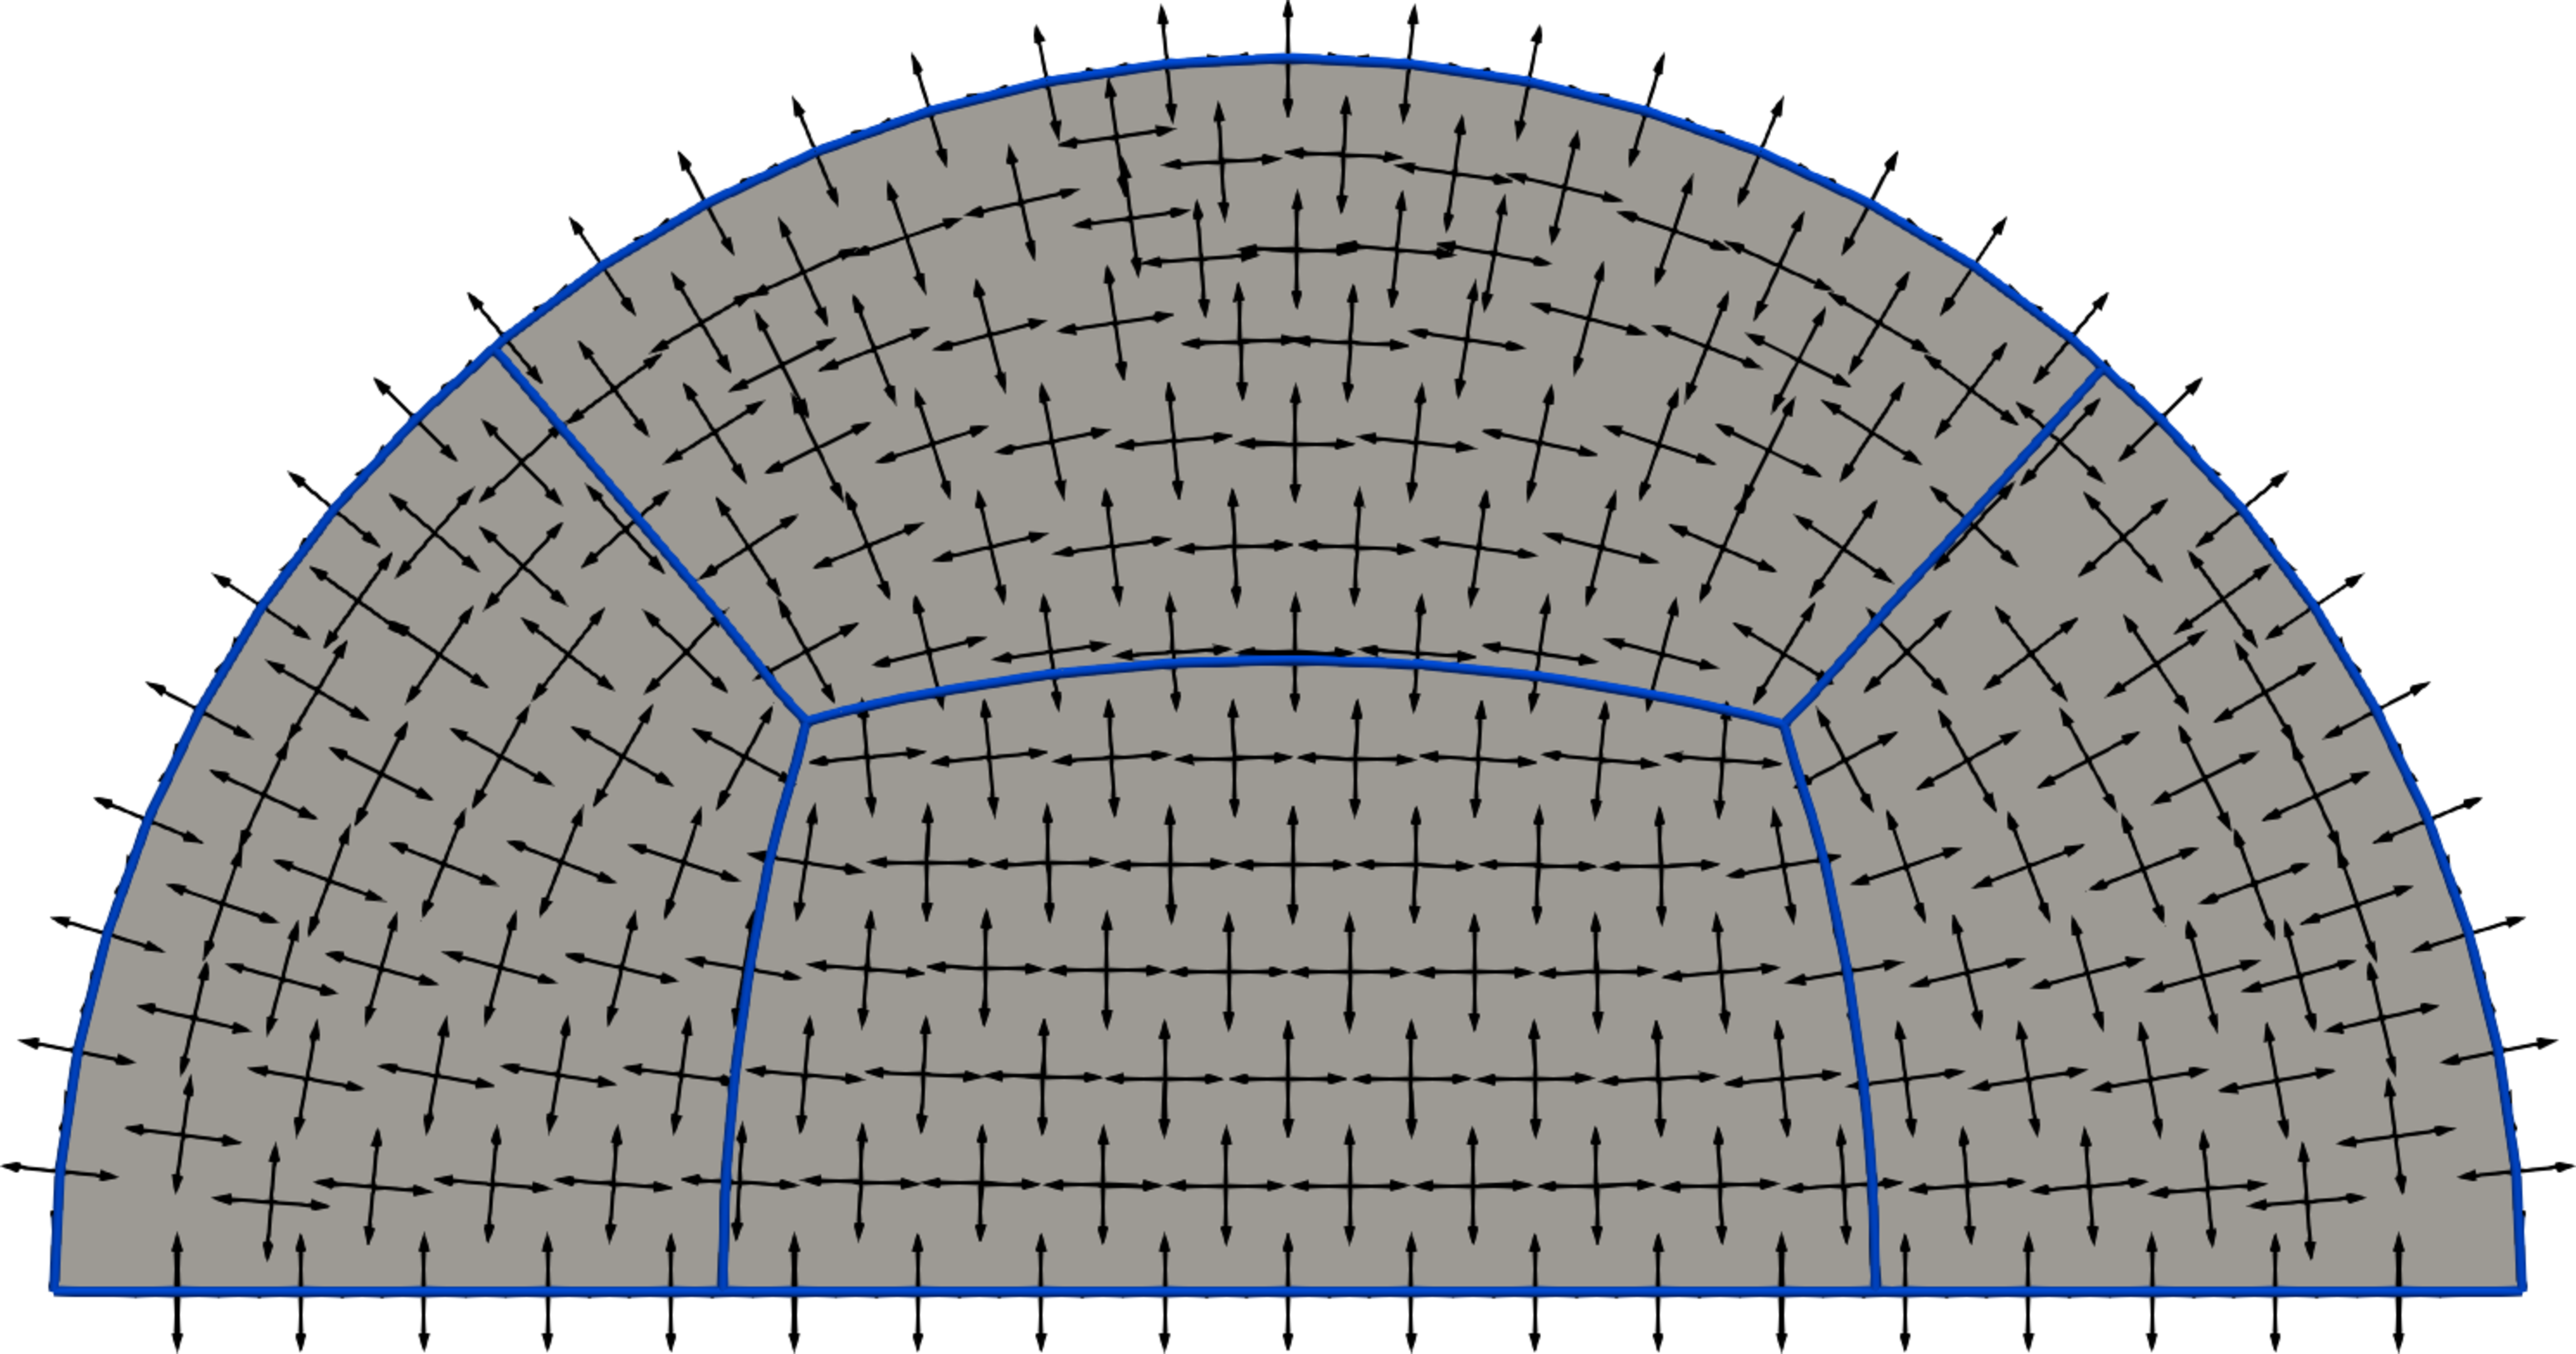
\includegraphics[width=\textwidth]{images/demi_disc_second_phi_first.pdf}
    \caption{Alignement du champ de croix présenté sur la figure \ref{fig:demiDisc_valProp_mauvaix_decoup} sur le bord du domaine et partitionnement du domaine.}
    \label{fig:demi_disc_second_cond_phi_first}
\end{subfigure}
\\[0.3ex]
\begin{subfigure}{0.65\textwidth}
    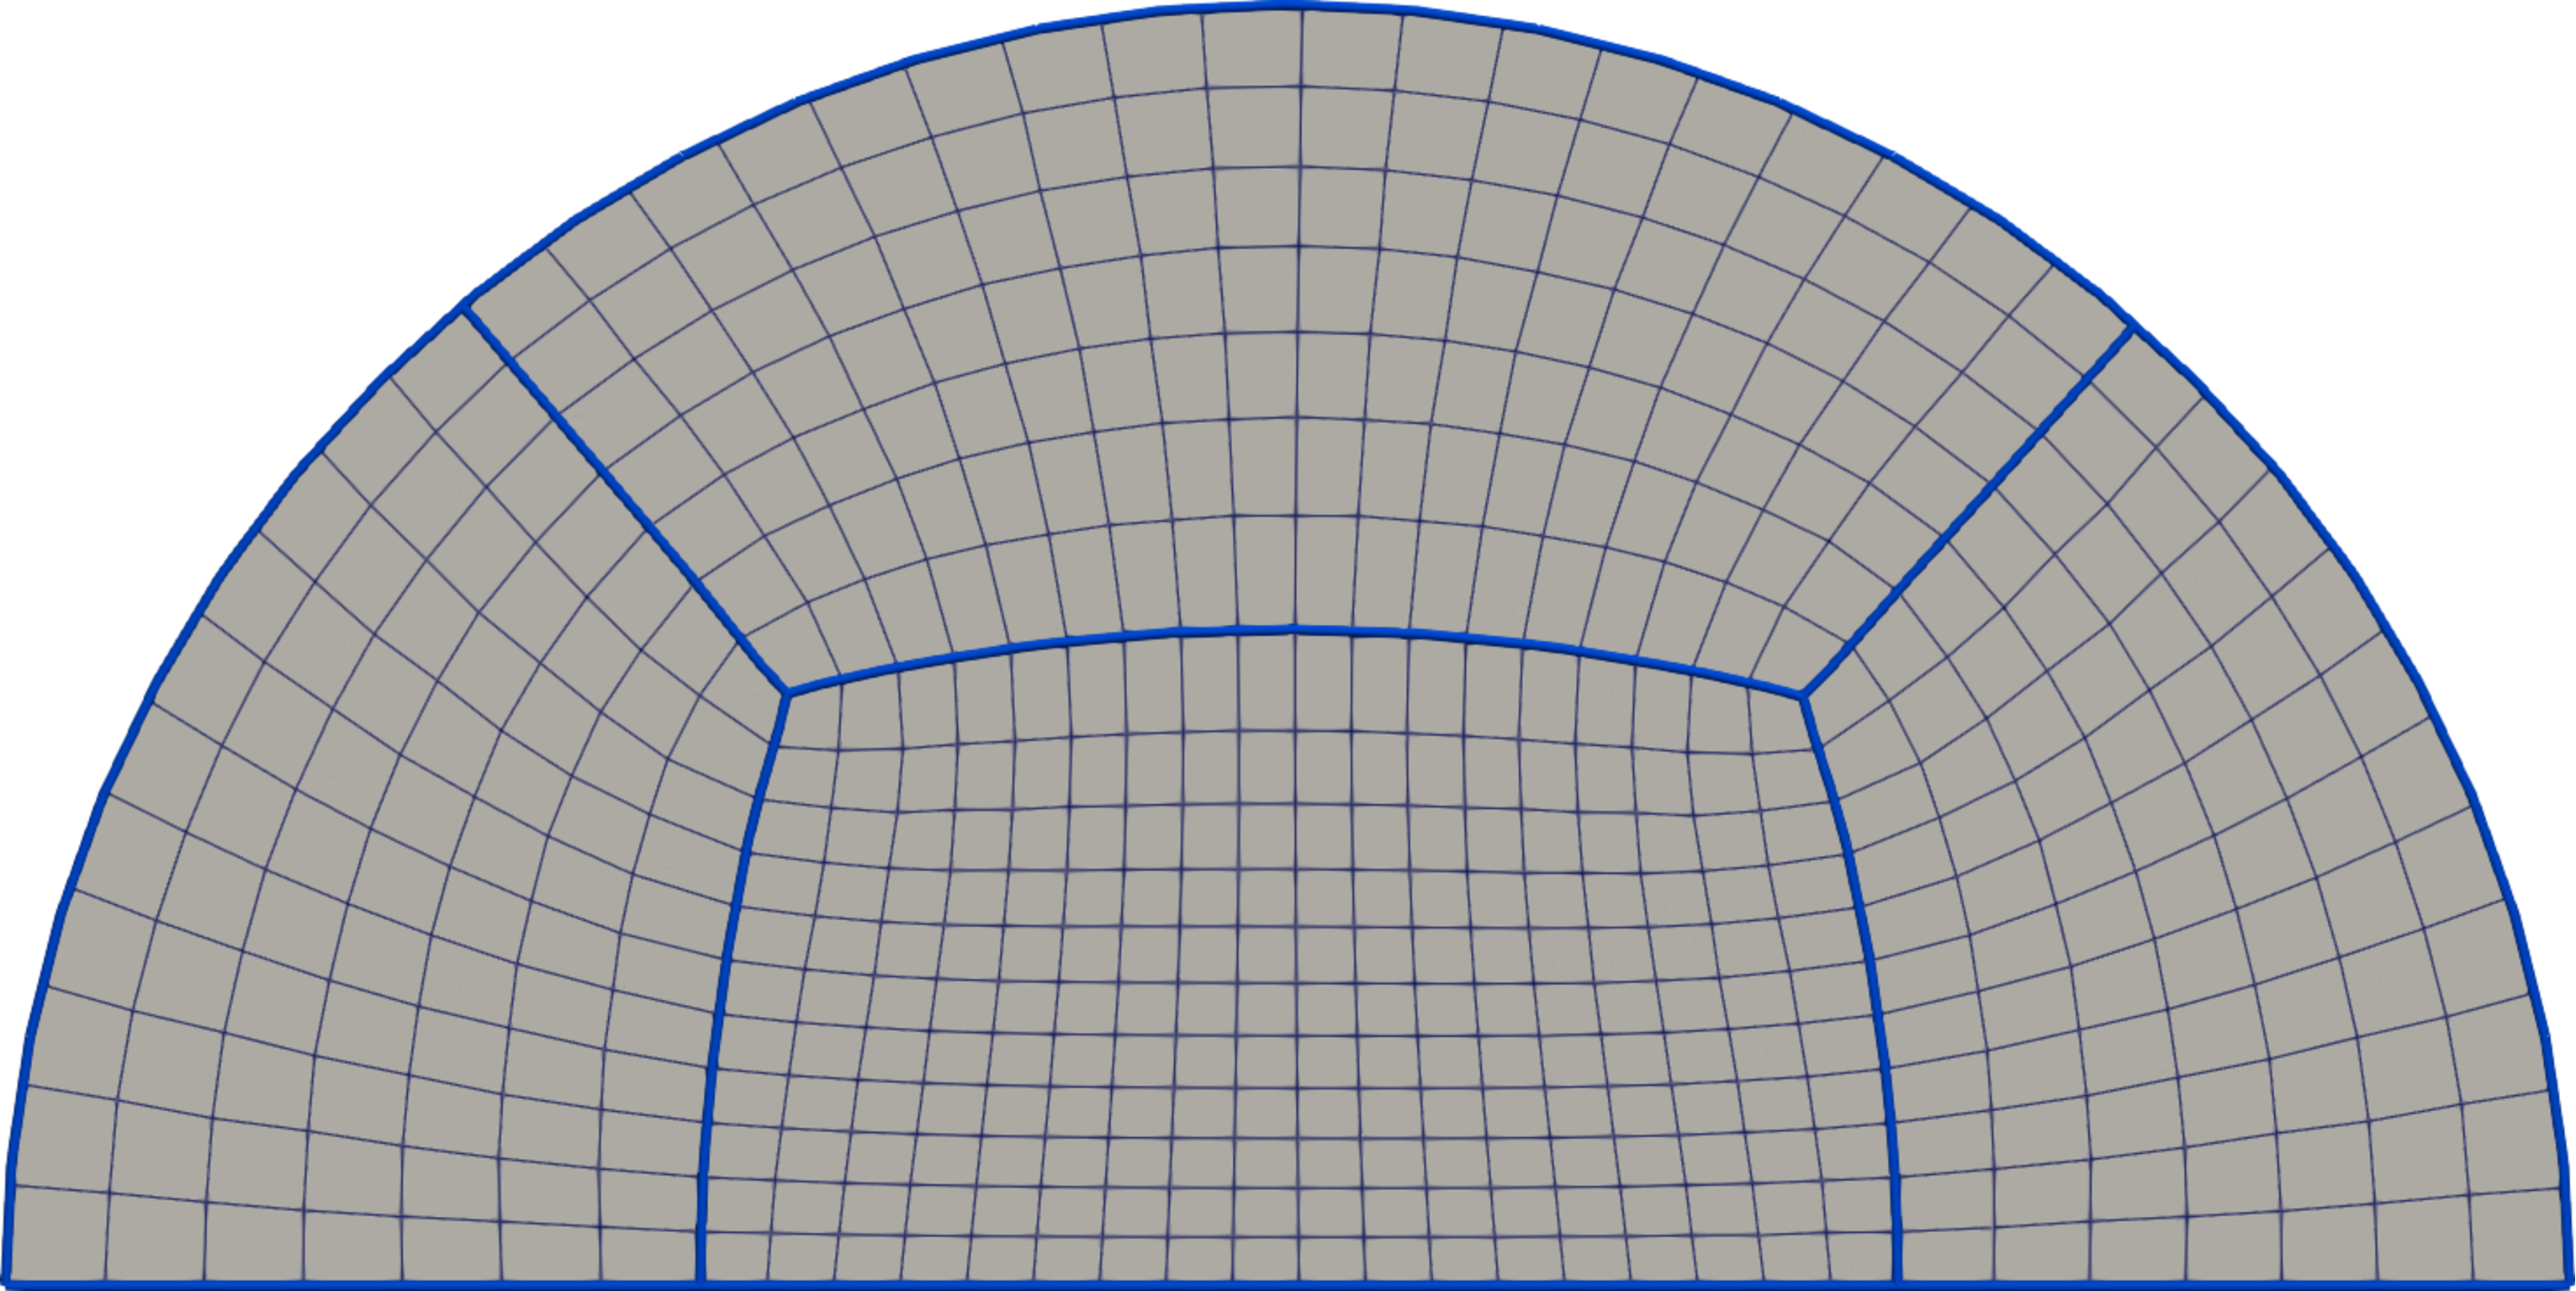
\includegraphics[width=\textwidth]{images/demi_disc_second_phi_second.pdf}
    \caption{Maillage quadrilatéral du domaine.}
    \label{fig:demi_disc_second_cond_phi_second}
\end{subfigure}
\caption{Illustration de l'opération d'alignement à partir du champ d'angle donné par l'équation \eqref{eqn:principe_def_phi}.}
\label{fig:demi_disc_second_cond_phi}
\end{figure}

\begin{remark}
    \[\]
    \vspace{-1cm}
    \begin{enumerate}
        \item On montre (voir le Théorème \ref{thm:theorem2}) que le champ de croix $\bar{v}$ est aligné par rapport à $\partial\Omega$. On se ramène ainsi au cas du champ de croix aligné sur le bord de $\Omega$ et l'application l'algorithme \ref{alg:algo_main} permet d'obtenir un partitionnement de $\Omega$ en régions de quatre côtés lorsque les séparatrices ne convergent pas en cycles limites.\\
        \item Le champ de croix $\bar{v}$ conserve certaines caractéristiques du champ de croix $\bar{u}$. Ainsi $\bar{v}$ est un champ de croix presque-$\mathcal{C}^1$ sur $\Omega$. De plus pour tout $p\in\Omega$, $id_{\bar{v}}(p)=id_{\bar{u}}(p)$ et pour tout $p\in\partial\Omega$, $id^\partial_{\bar{v}}(p)=I_p$.\\
        \item La condition \eqref{eqn:principe_hypothese_u} permet de garantir que $\phi(\gamma(1))-\phi(\gamma(0))=0$ (voir le lemme \ref{lem:marvelous_lemma}) nécessaire pour garantir que le point $p=\gamma(0)=\gamma(1)$ satisfait $id_{\bar{v}}(p)=I_p$.%integrale dphi egale 0 car hypothese sur u garantissant ainsi idv=I Controle on trouve ce qui est prescrit on peut donc evider des quadrangle degenerer en choisissant le bon I en fonction la courbure locale en chaque point
    \end{enumerate}
\end{remark}

 L'algorithme suivant résume le procédé.

\vspace{0.5cm}
\begin{algorithm}[H]
\label{alg:algo_simply_connected}
\SetKwInOut{Input}{Entrée}
\SetKwInOut{Output}{Sortie}
\Input{$\Omega$ un domaine borné et fermé simplement connexe, champ de croix $\bar{u}$ défini sur $\Omega$, ensemble $\mathcal{B}$, paramètre $I(p)$ pour tout $p\in\partial\Omega$.}
\Output{Partition de $\Omega$ en ensembles de régions.}
\vspace{0.2cm}
1.) Calcul du champ d'alignement (voir l'équation \eqref{eqn:principe_def_phi}),\\\vspace{0.2cm}
2.) Calcul du champ de croix $\bar{v}$ (voir l'équation \eqref{eqn:principe_def_v}),\\\vspace{0.2cm}
3.) Application de l'algorithme \ref{alg:algo_main} au champ de croix $\bar{v}$.\\\vspace{0.2cm}
\caption{Algorithme de partitionnement pour un domaine simplement connexe basé sur un champ de croix non aligné}
\end{algorithm}
\vspace{0.5cm}

En appliquant cet algorithme au champ de croix représenté sur la figure \ref{fig:demiDisc_valProp_mauvaix_decoup}, nous obtenons le partitionnement illustré sur la figure \ref{fig:demi_disc_second_cond_phi}. Un autre exemple est présenté sur la figure \ref{fig:rect_demi_disc}. Dans ce cas, le champ de croix initial possède deux points singuliers d'indice $-1/4$. L'ensemble $\mathcal{B}$ correspond aux coins du domaine, auxquels nous avons associé le paramètre $I_p=1/4$ pour tout $p\in\mathcal{B}$.



\begin{figure}[!h]
\centering
\begin{subfigure}{0.58\textwidth}
    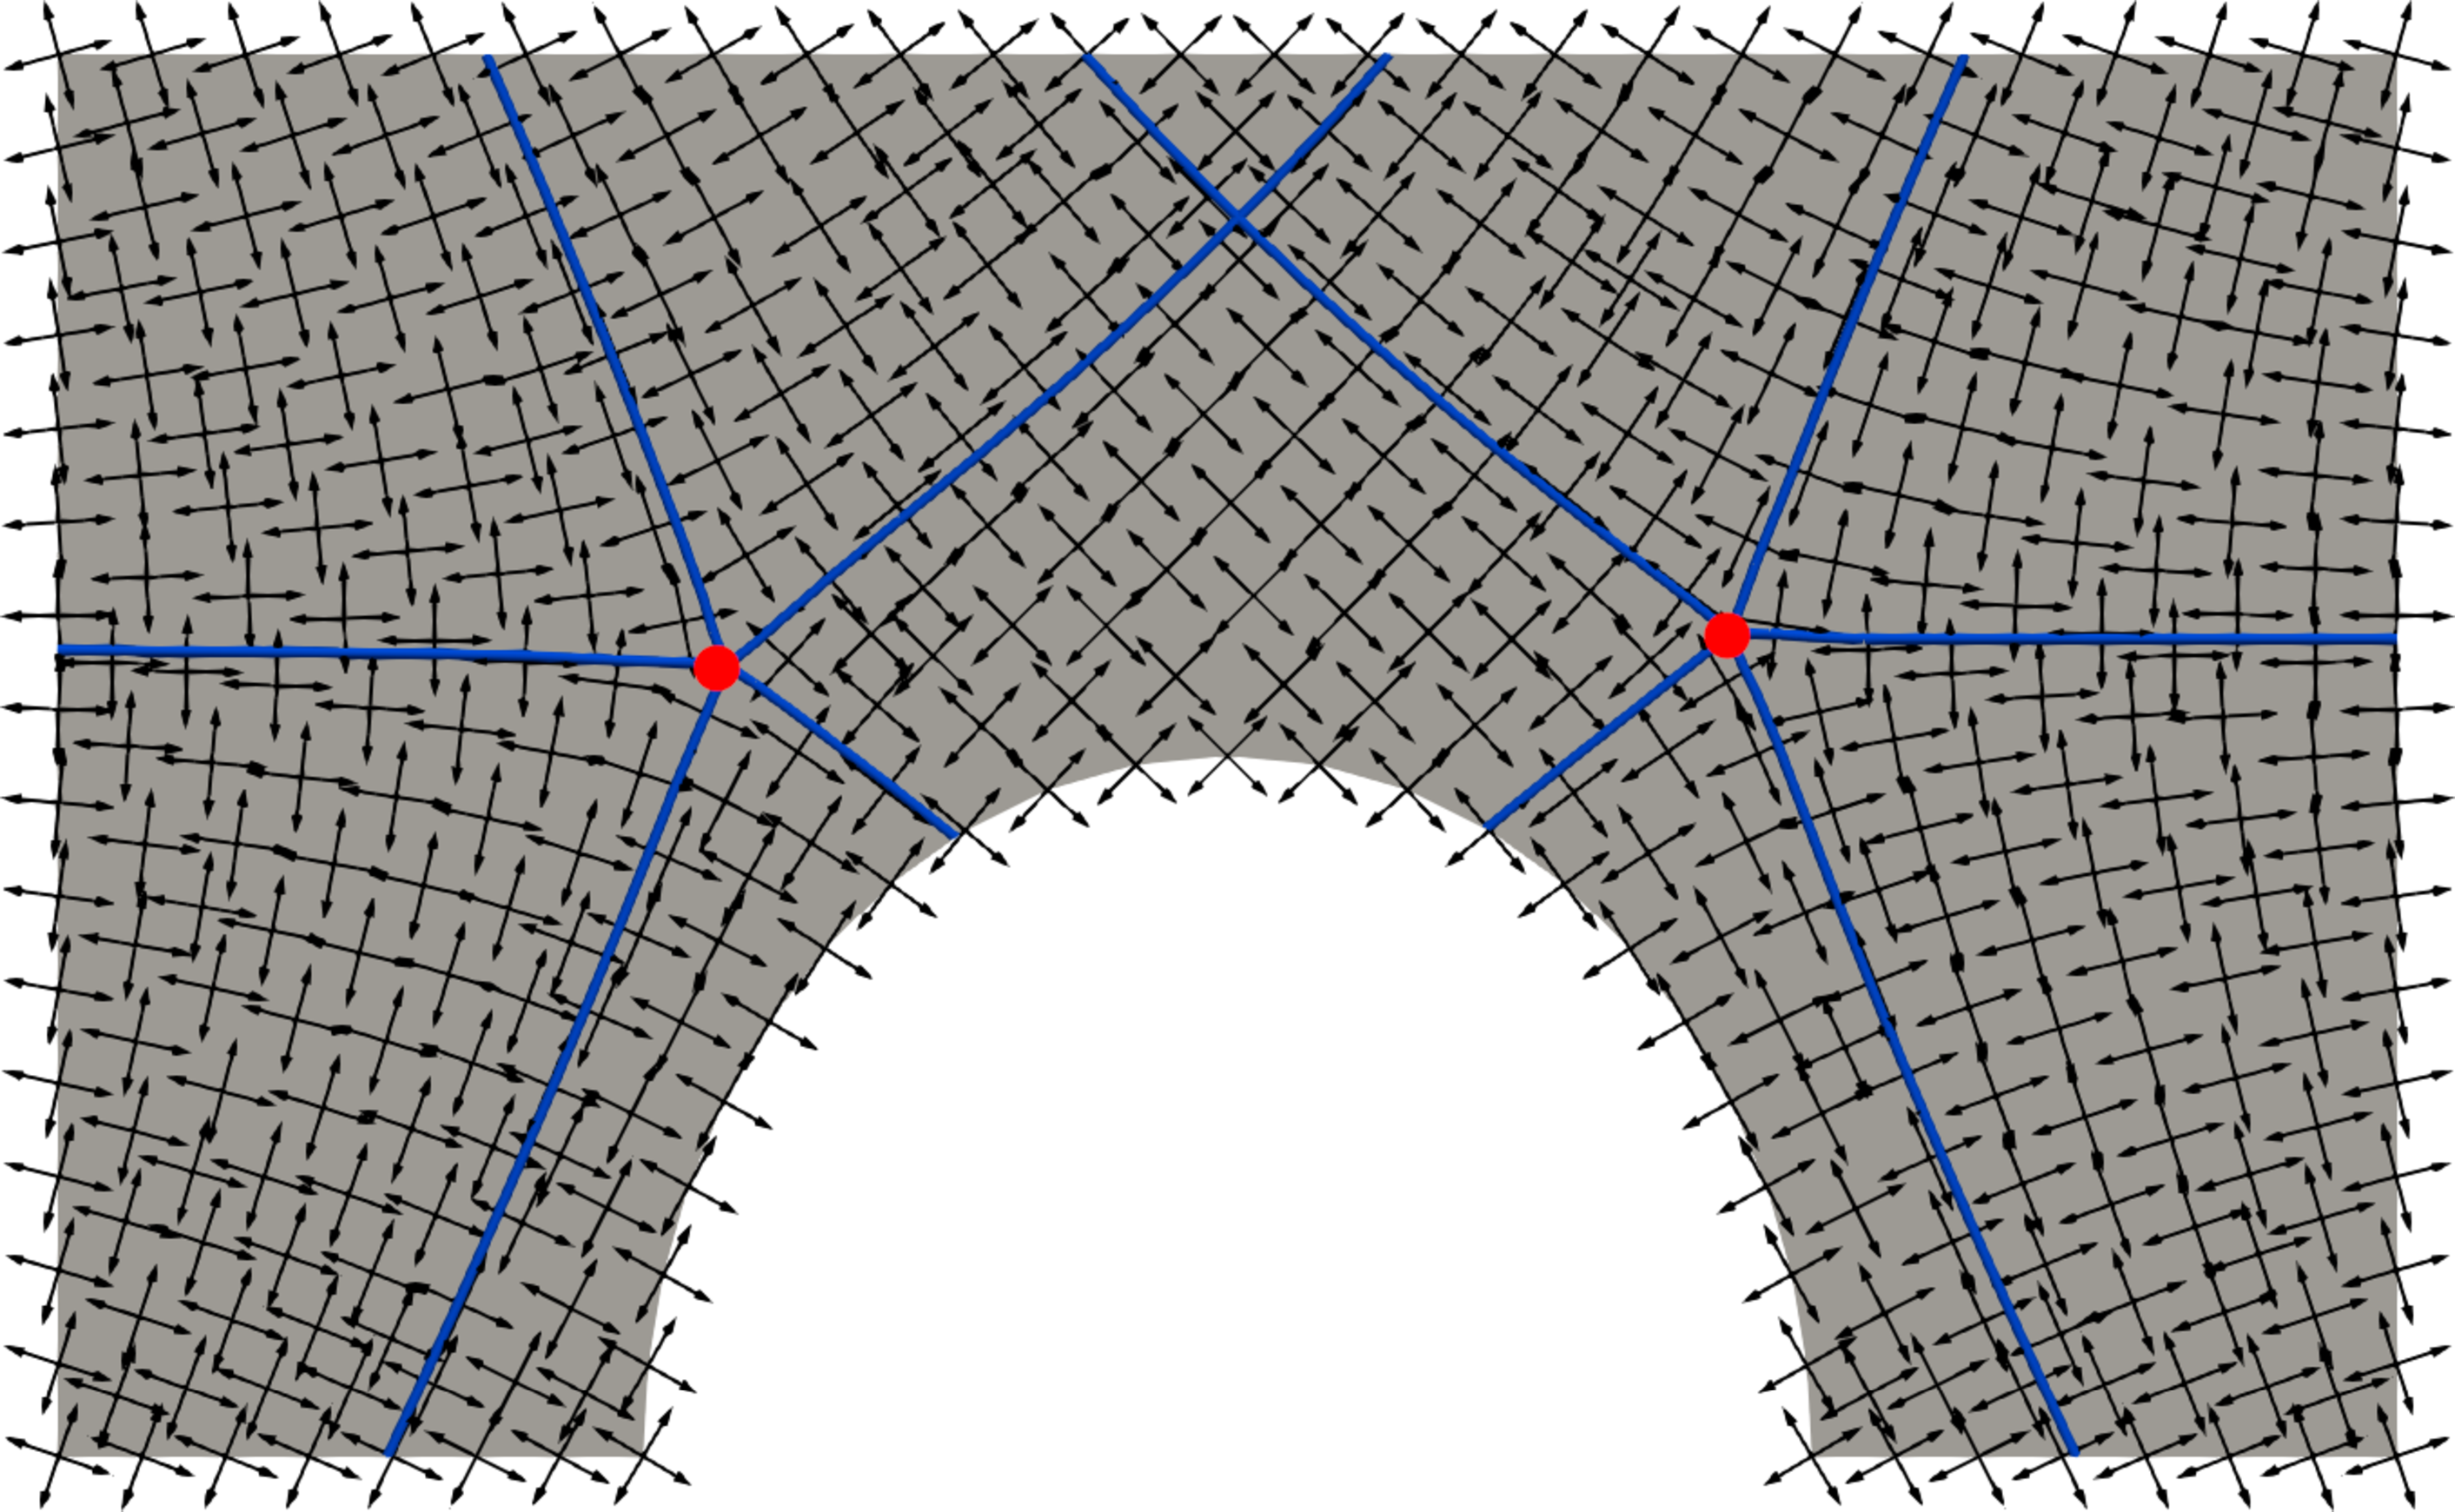
\includegraphics[width=\textwidth]{images/rect_demi_disc_first.pdf}
    \caption{Champ de croix initial avec deux points singuliers internes d'indice $1/4$.}
    \label{fig:rect_demi_disc_first}
\end{subfigure}
\\[0.46cm]
\begin{subfigure}{0.58\textwidth}
    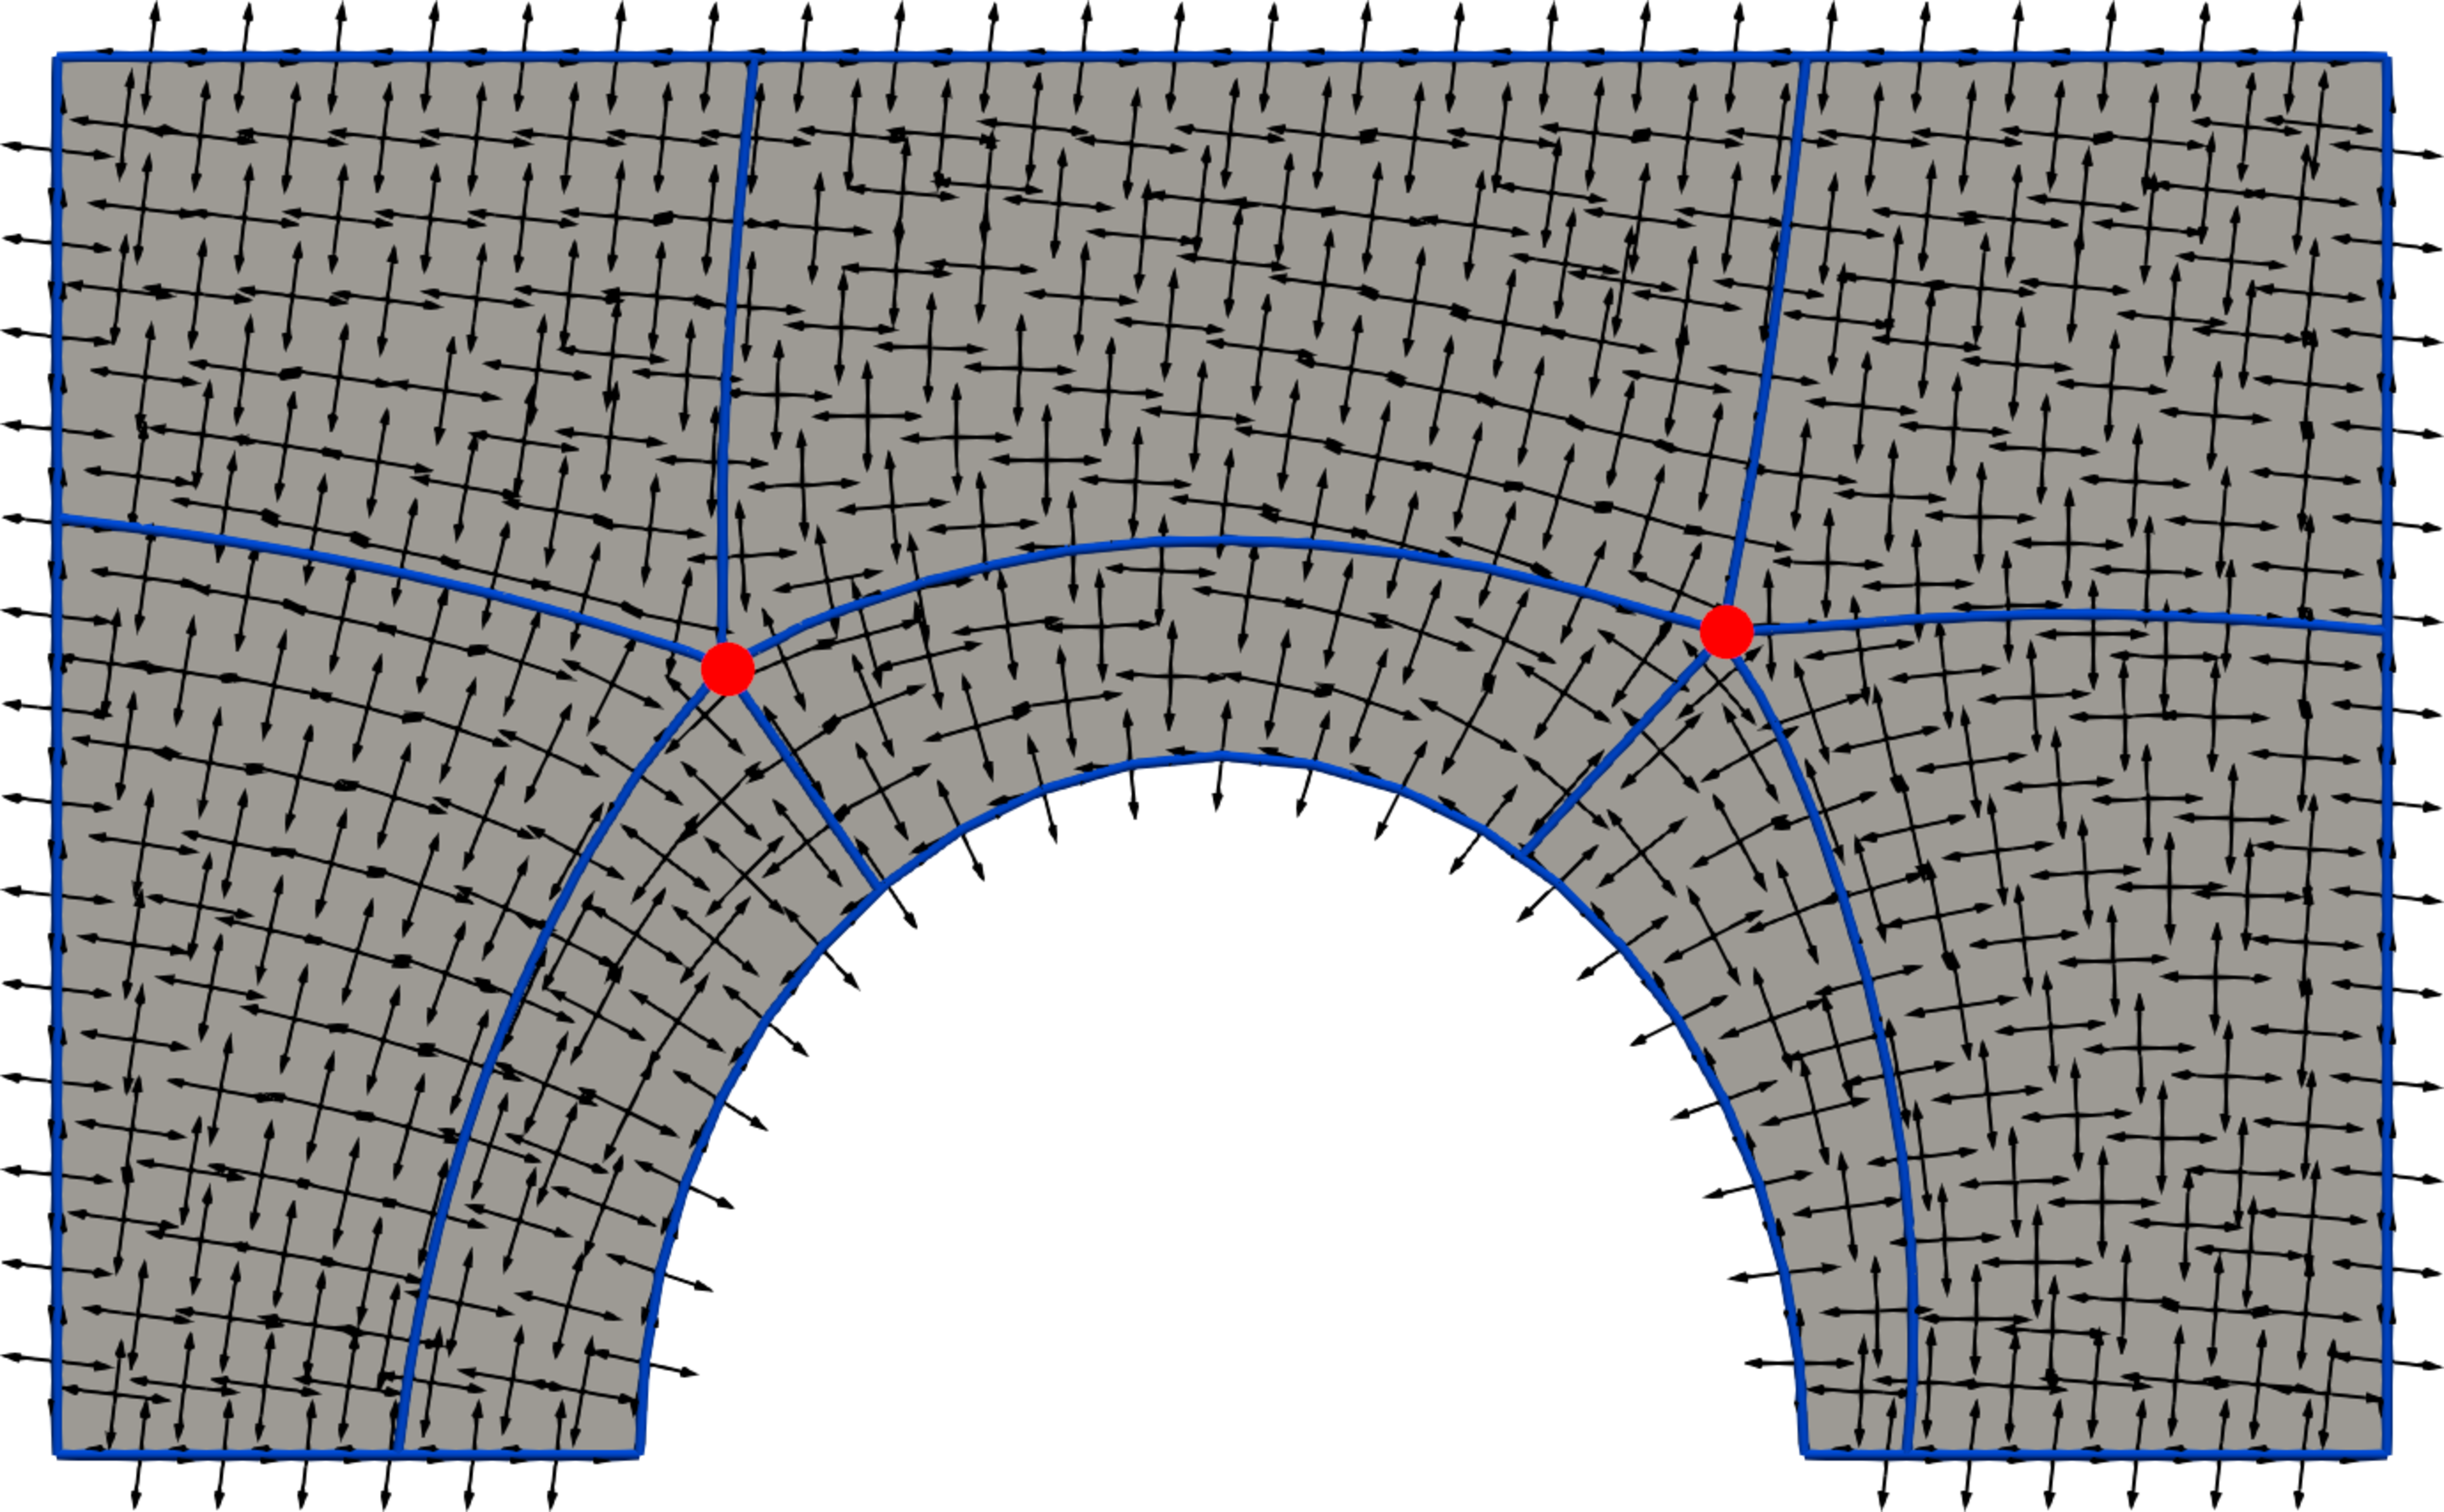
\includegraphics[width=\textwidth]{images/rect_demi_disc_second.pdf}
    \caption{Alignement du champ de croix initial sur le bord du domaine et partitionnement du domaine.}
    \label{fig:rect_demi_disc_second}
\end{subfigure}
\\[0.46cm]
\begin{subfigure}{0.58\textwidth}
    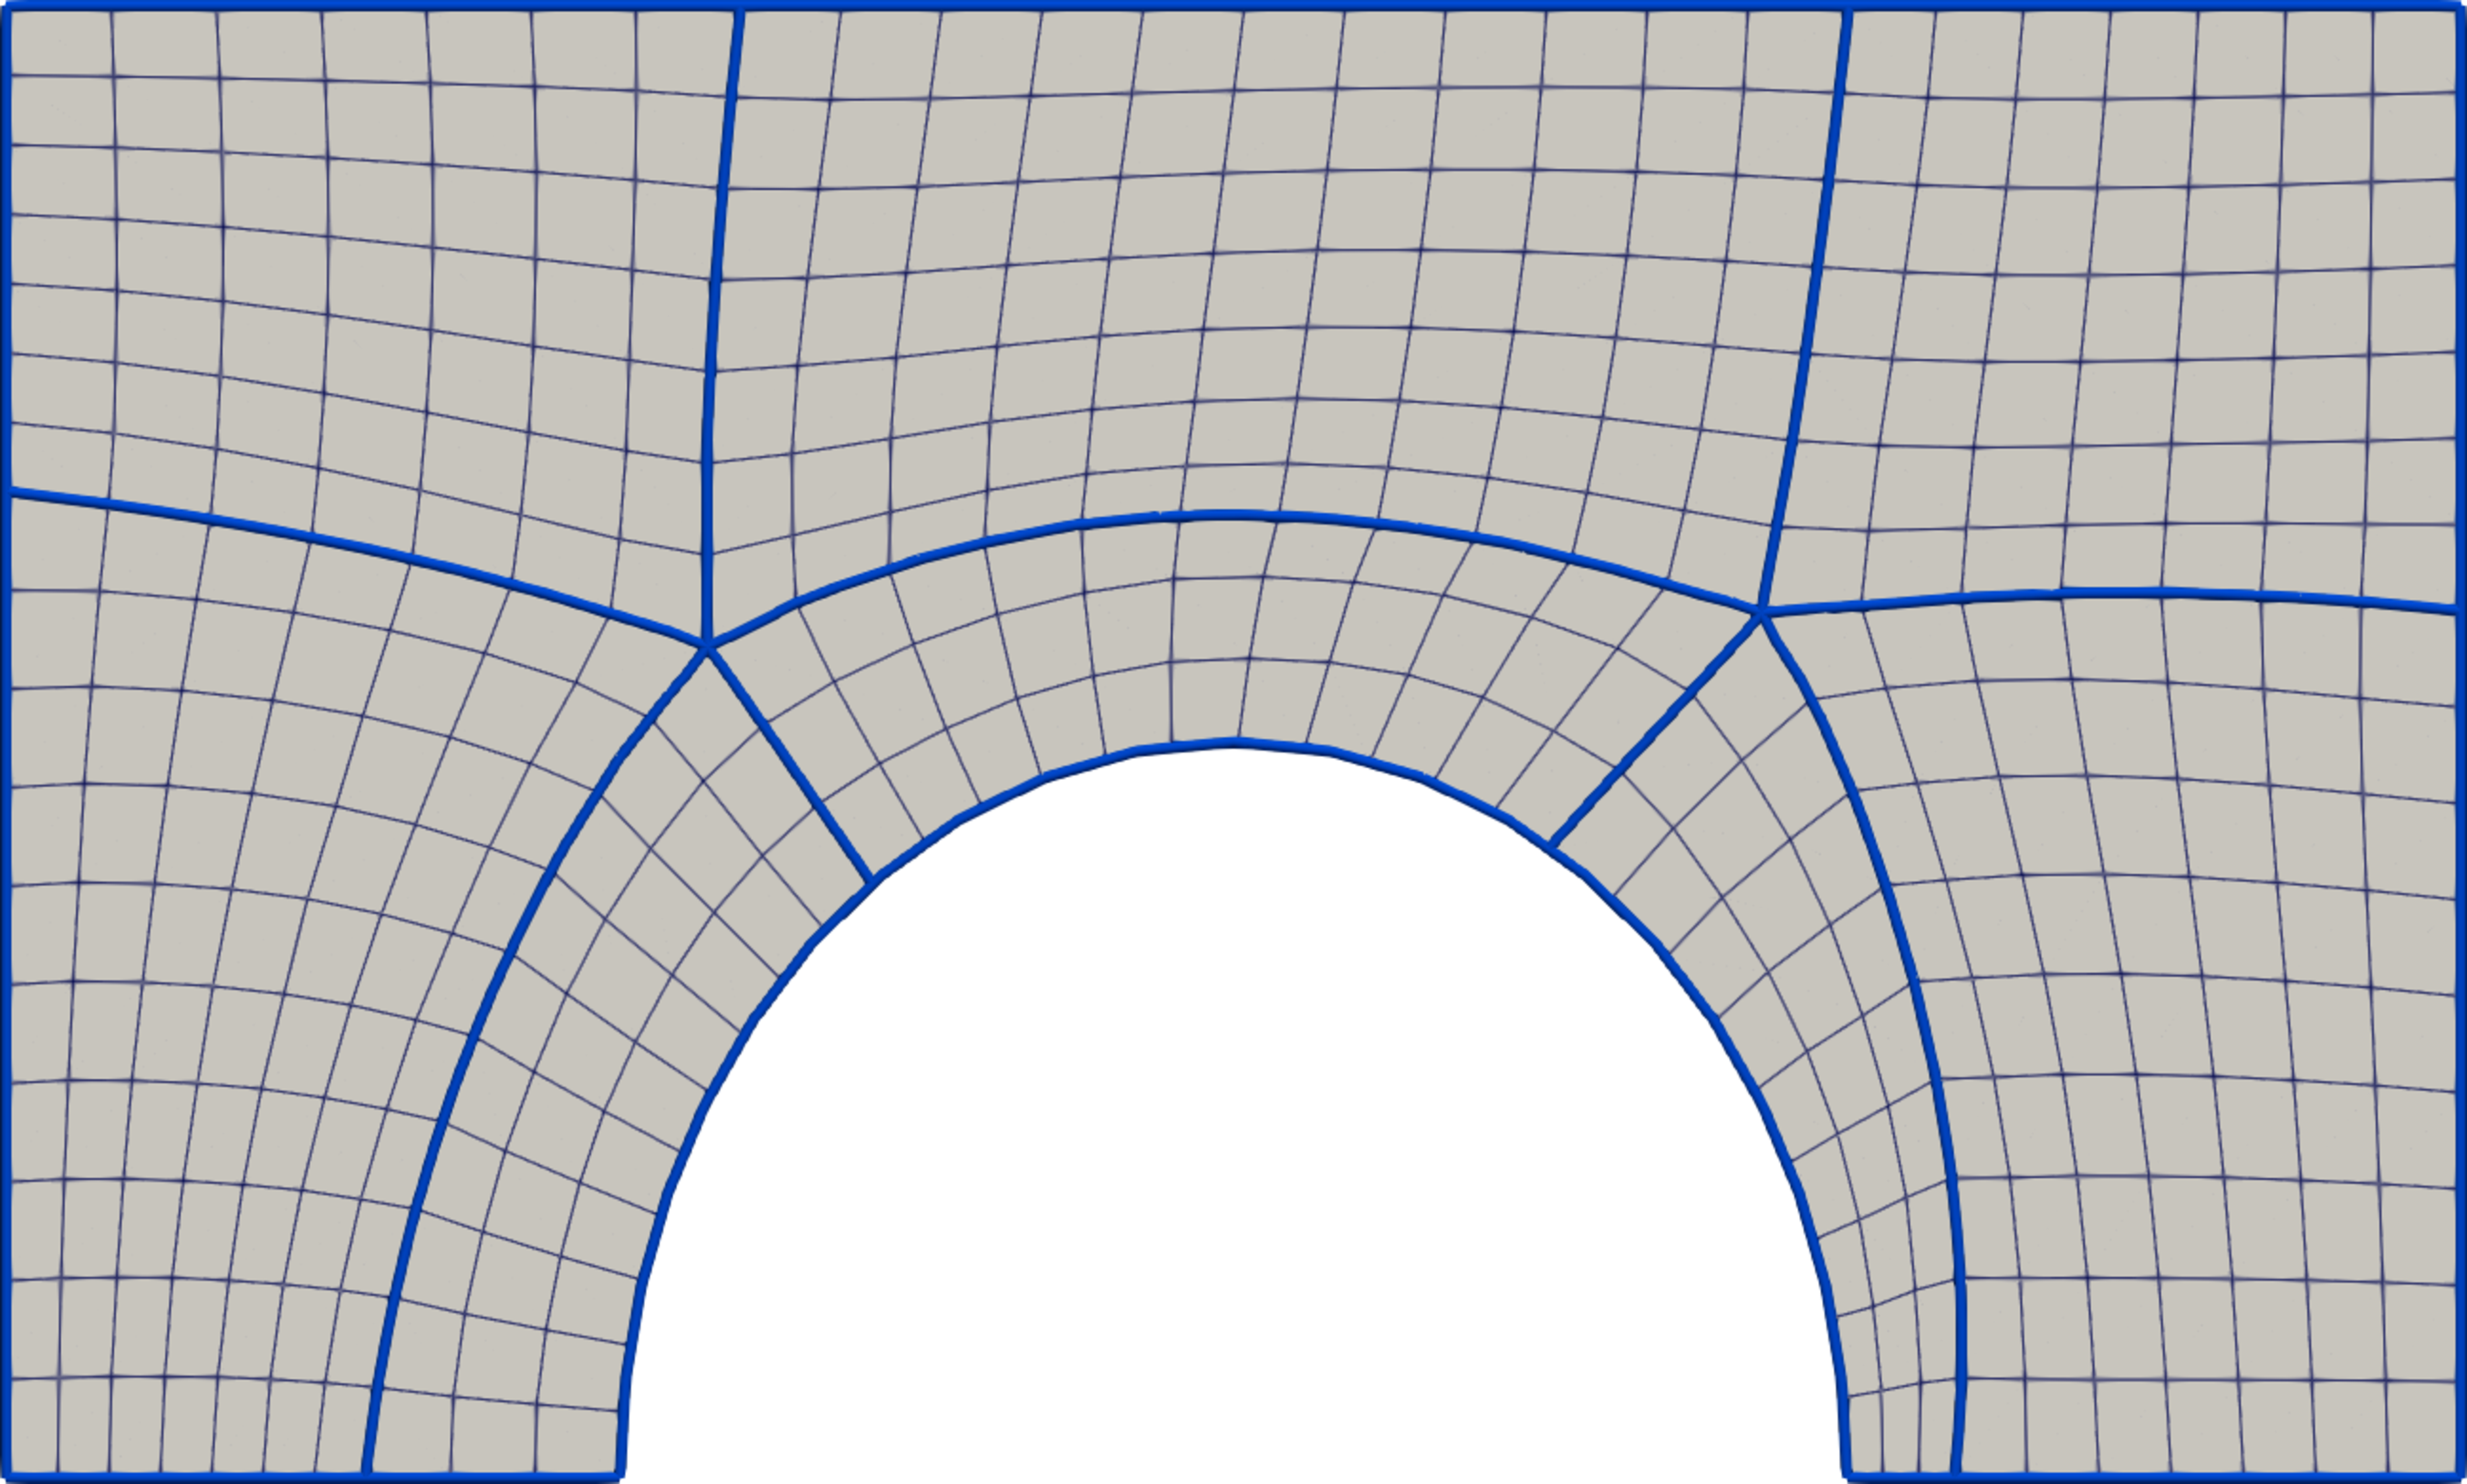
\includegraphics[width=\textwidth]{images/rect_demi_disc_third.pdf}
    \caption{Maillage quadilatéral du domaine présentant un quadrangle dégénéré.}
    \label{fig:rect_demi_disc_third}
\end{subfigure}

\caption{Une autre illustration de l'opération d'alignement à partir du champ d'angle donné.}
\label{fig:rect_demi_disc}
\end{figure}

\paragraph{Domaine non-simplement connexe:}
Nous supposons maintenant que $\Omega$ est un domaine non-simplement connexe. Autrement dit sa frontière $\partial\Omega$ peut potentiellement être constitué de plusieurs composantes connexes. On a donc $\partial\Omega=\cup_i\Gamma_i$, où $\Gamma_i,~i\in\llbracket 0, n_b-1\rrbracket$ désigne les composantes connexes de $\partial\Omega$ et $n_b$ le nombre de composantes connexes de $\partial\Omega$. Pour tout $i\in\llbracket0, n_b-1\rrbracket$, on note $\gamma_i$ la paramétrisation de $\Gamma_i$ sur $[0, 1]$ dans le sens positif. Soit $\bar{u}$ un champ de croix presque-$\mathcal{C}^1$ défini sur $\Omega$ et non-nécessairement aligné sur le bord de $\Omega$ tel que $0<\#\mathcal{S}_{\bar{u}}<\infty$ et pour tout point $p\in\mathcal{S}_{\bar{u}}\backslash\partial\Omega$, $id_{\bar{u}}(p)=k/4$, avec $k\in\mathbb{Z}$ et $k\leq 1$. En appliquant le processus présenté dans la partie précédente, la condition \eqref{eqn:principe_hypothese_u} devient:

\begin{equation}
    \sum_{i=0}^{n_b-1}\left(\theta_{\bar{u}}^{\gamma_i}(1)-\theta_{\bar{u}}^{\gamma_i}(0)\right)=2\pi\chi(\Omega)-2\pi\sum_{p\in\mathcal{B}}I_p.
    \label{eqn:principe_hypothese_u_prime}
\end{equation}
Cependant, cette condition ne permet pas de garantir que, pour tout $i\in\llbracket0, n_b-1\rrbracket$, $\phi(\gamma_i(1))-\phi(\gamma_i(0))=0$, ce qui est essentiel pour s'assurer que pour tout $p\in\partial \Omega$, $id_{\bar{v}}(p)= I_p$. C'est notamment ce qu'on observe sur l'exemple de la figure \ref{fig:carre_demi_disc_vide_mauvais}. Sur cet exemple, le champ de croix initial vérifie la condition \eqref{eqn:principe_hypothese_u_prime}. Elle contient deux points singuliers internes, chacun ayant un indice de $-1/4$. L'ensemble $\mathcal{B}$ se compose, d'une part, des quatre coins du bord carré où chaque coin a un paramètre $I_p$ fixé à $1/4$, et d'autre part, des deux coins du demi-disque où chaque coin a un paramètre $I_p$ fixé à $-1/4$. Le champ d'alignement est calculé avec l'équation \eqref{eqn:first_phi_computation}, puis le champ de croix $\bar{v}$ est construit. On observe clairement que $\bar{v}$ est bien aligné avec le bord du domaine et conserve les singularités internes du champ de croix initial. Cependant, on remarque l'apparition de singularités de bord dans le champ de croix $\bar{v}$. En appliquant l'algorithme de partitionnement \ref{alg:algo_main} sur $\bar{v}$, le partitionnement obtenu présente des régions à quatre côtés (figure \ref{fig:carre_demi_disc_vide_mauvais_second}) mais, la présence de points singuliers de bord non contrôlés (en termes de positionnement et d'indice) conduit à un maillage quadrilatéral comportant des quadrangles dégénérés (figure \ref{fig:carre_demi_disc_vide_mauvais_third}).

\begin{figure}[!h]
\centering
\begin{subfigure}{0.495\textwidth}
    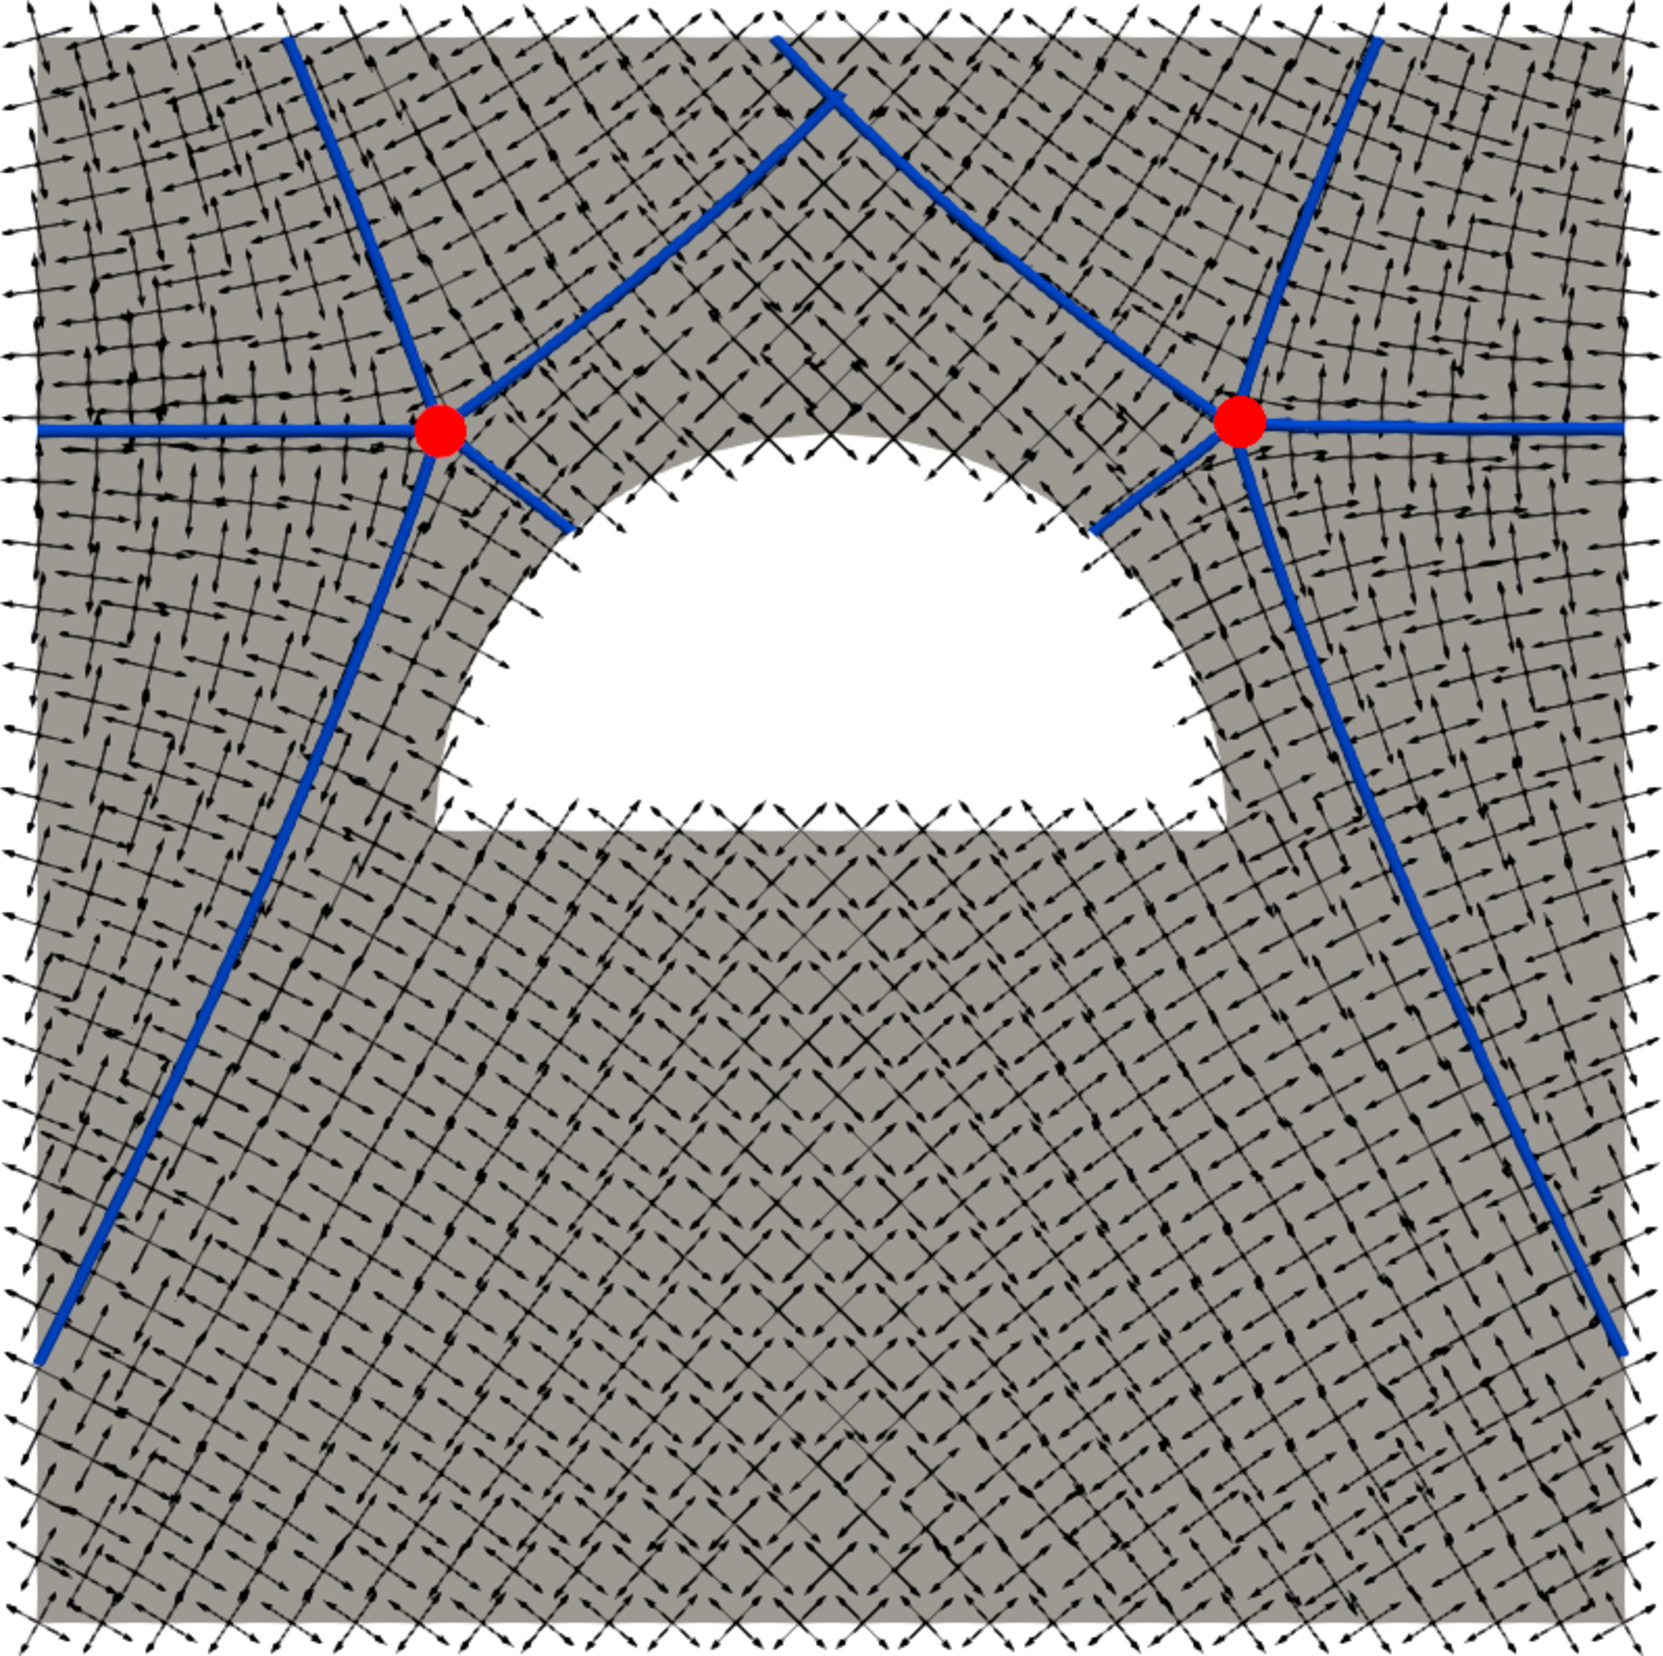
\includegraphics[width=\textwidth]{images/carre_demi_disc_vide_mauvais_first.pdf}
    \caption{Champ de croix initial avec deux points singuliers internes, chacun d'indice $1/4$ et vérifiant l'équation \ref{eqn:principe_hypothese_u_prime}.}
    \label{fig:carre_demi_disc_vide_mauvais_first}
\end{subfigure}
\hfill
\begin{subfigure}{0.495\textwidth}
    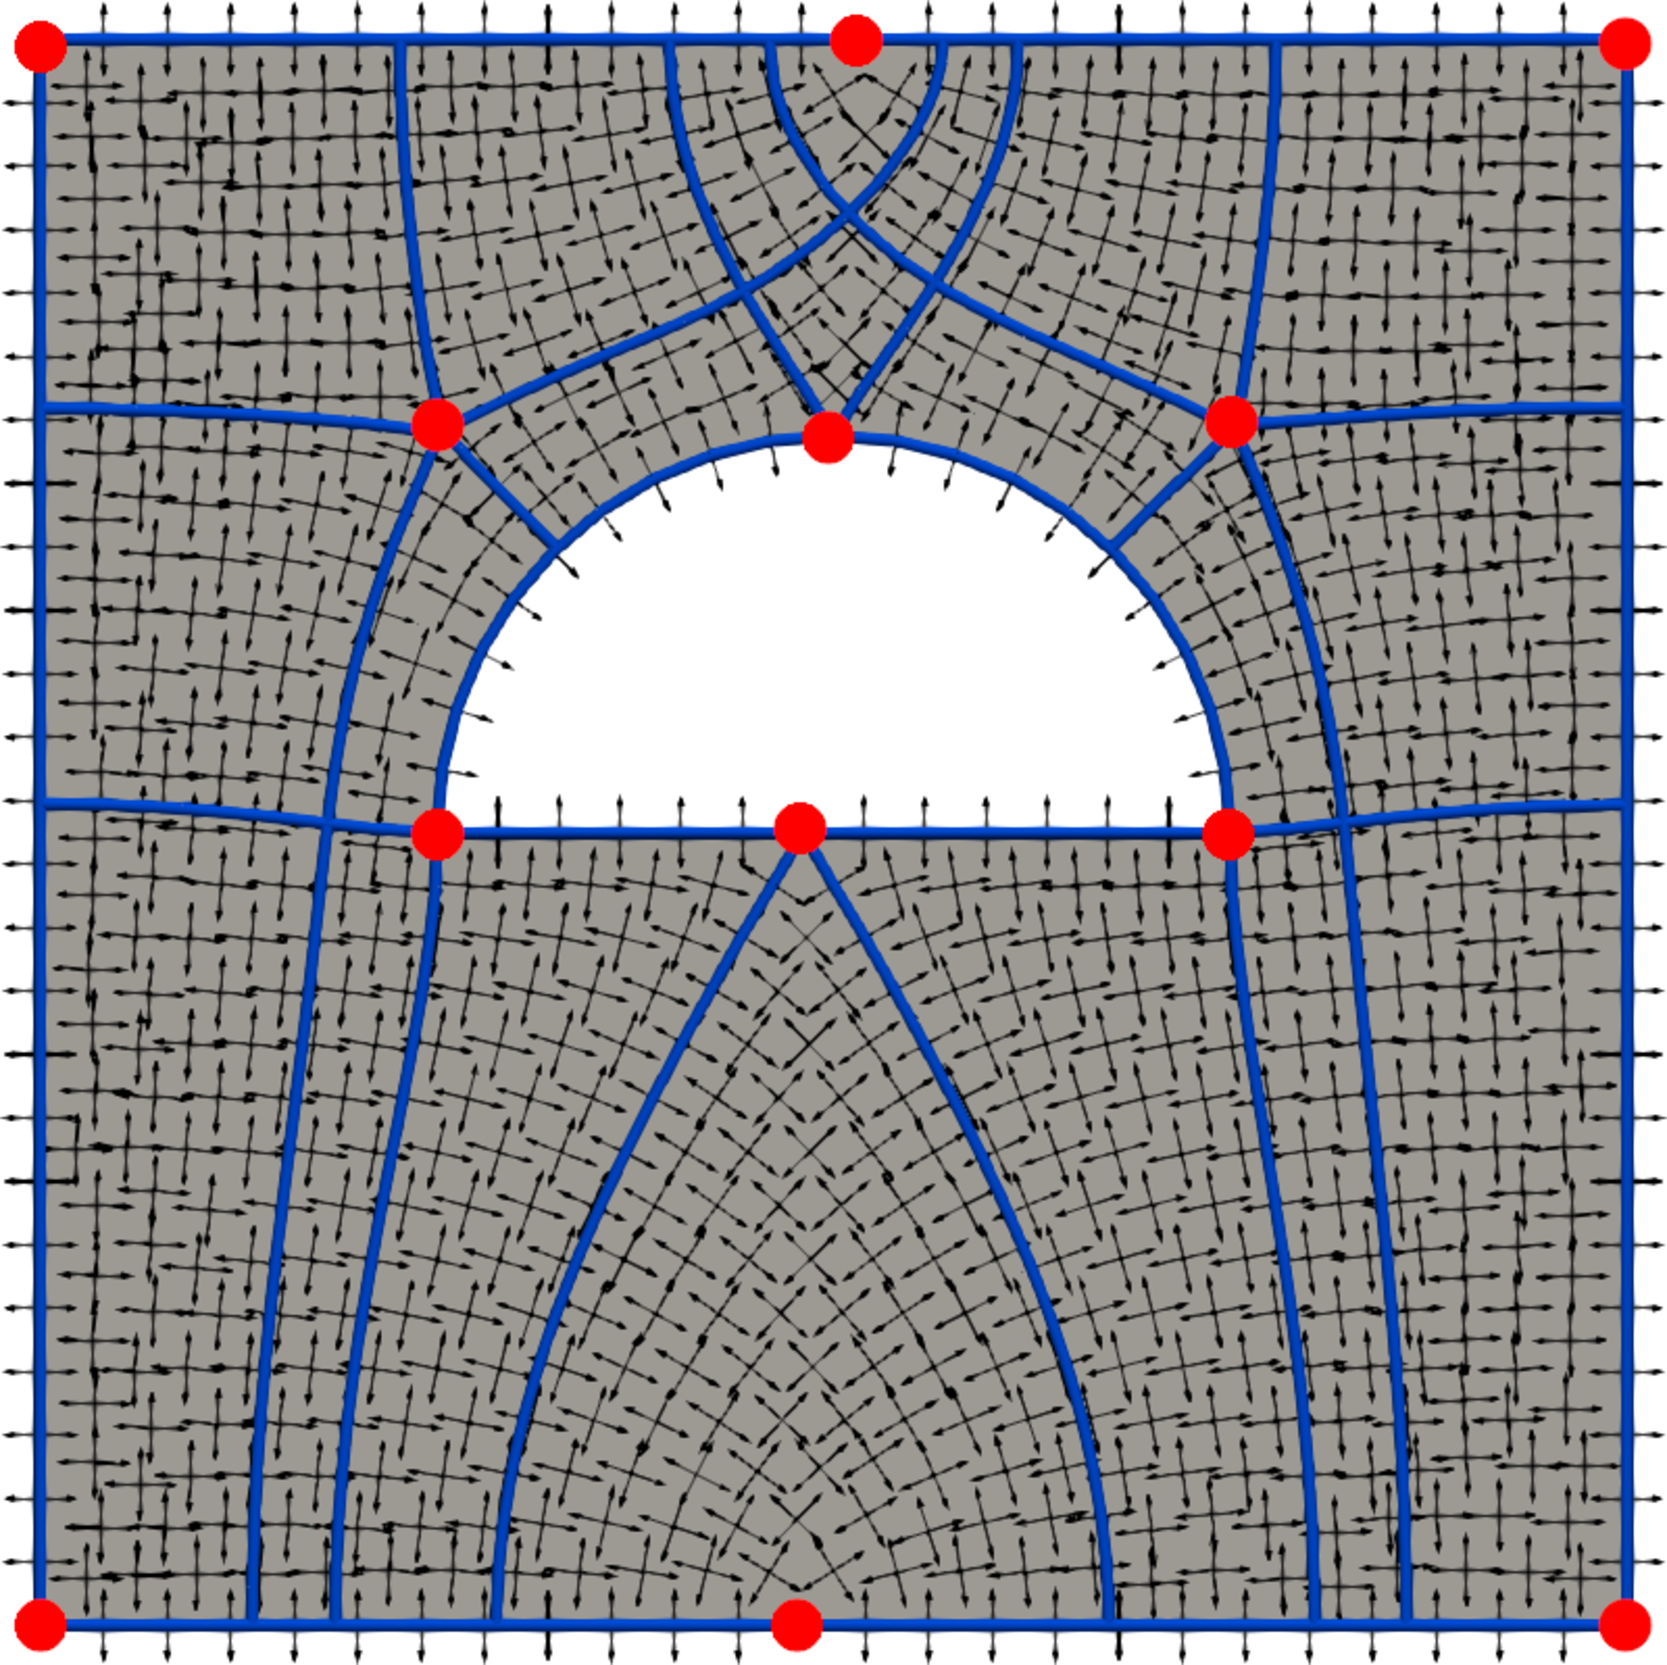
\includegraphics[width=\textwidth]{images/carre_demi_disc_vide_mauvais_second.pdf}
    \caption{Alignement du champ de croix initial sur le bord du domaine et partitionnement du domaine.}
    \label{fig:carre_demi_disc_vide_mauvais_second}
\end{subfigure}
\\[0.2cm]
\begin{subfigure}{0.5\textwidth}
    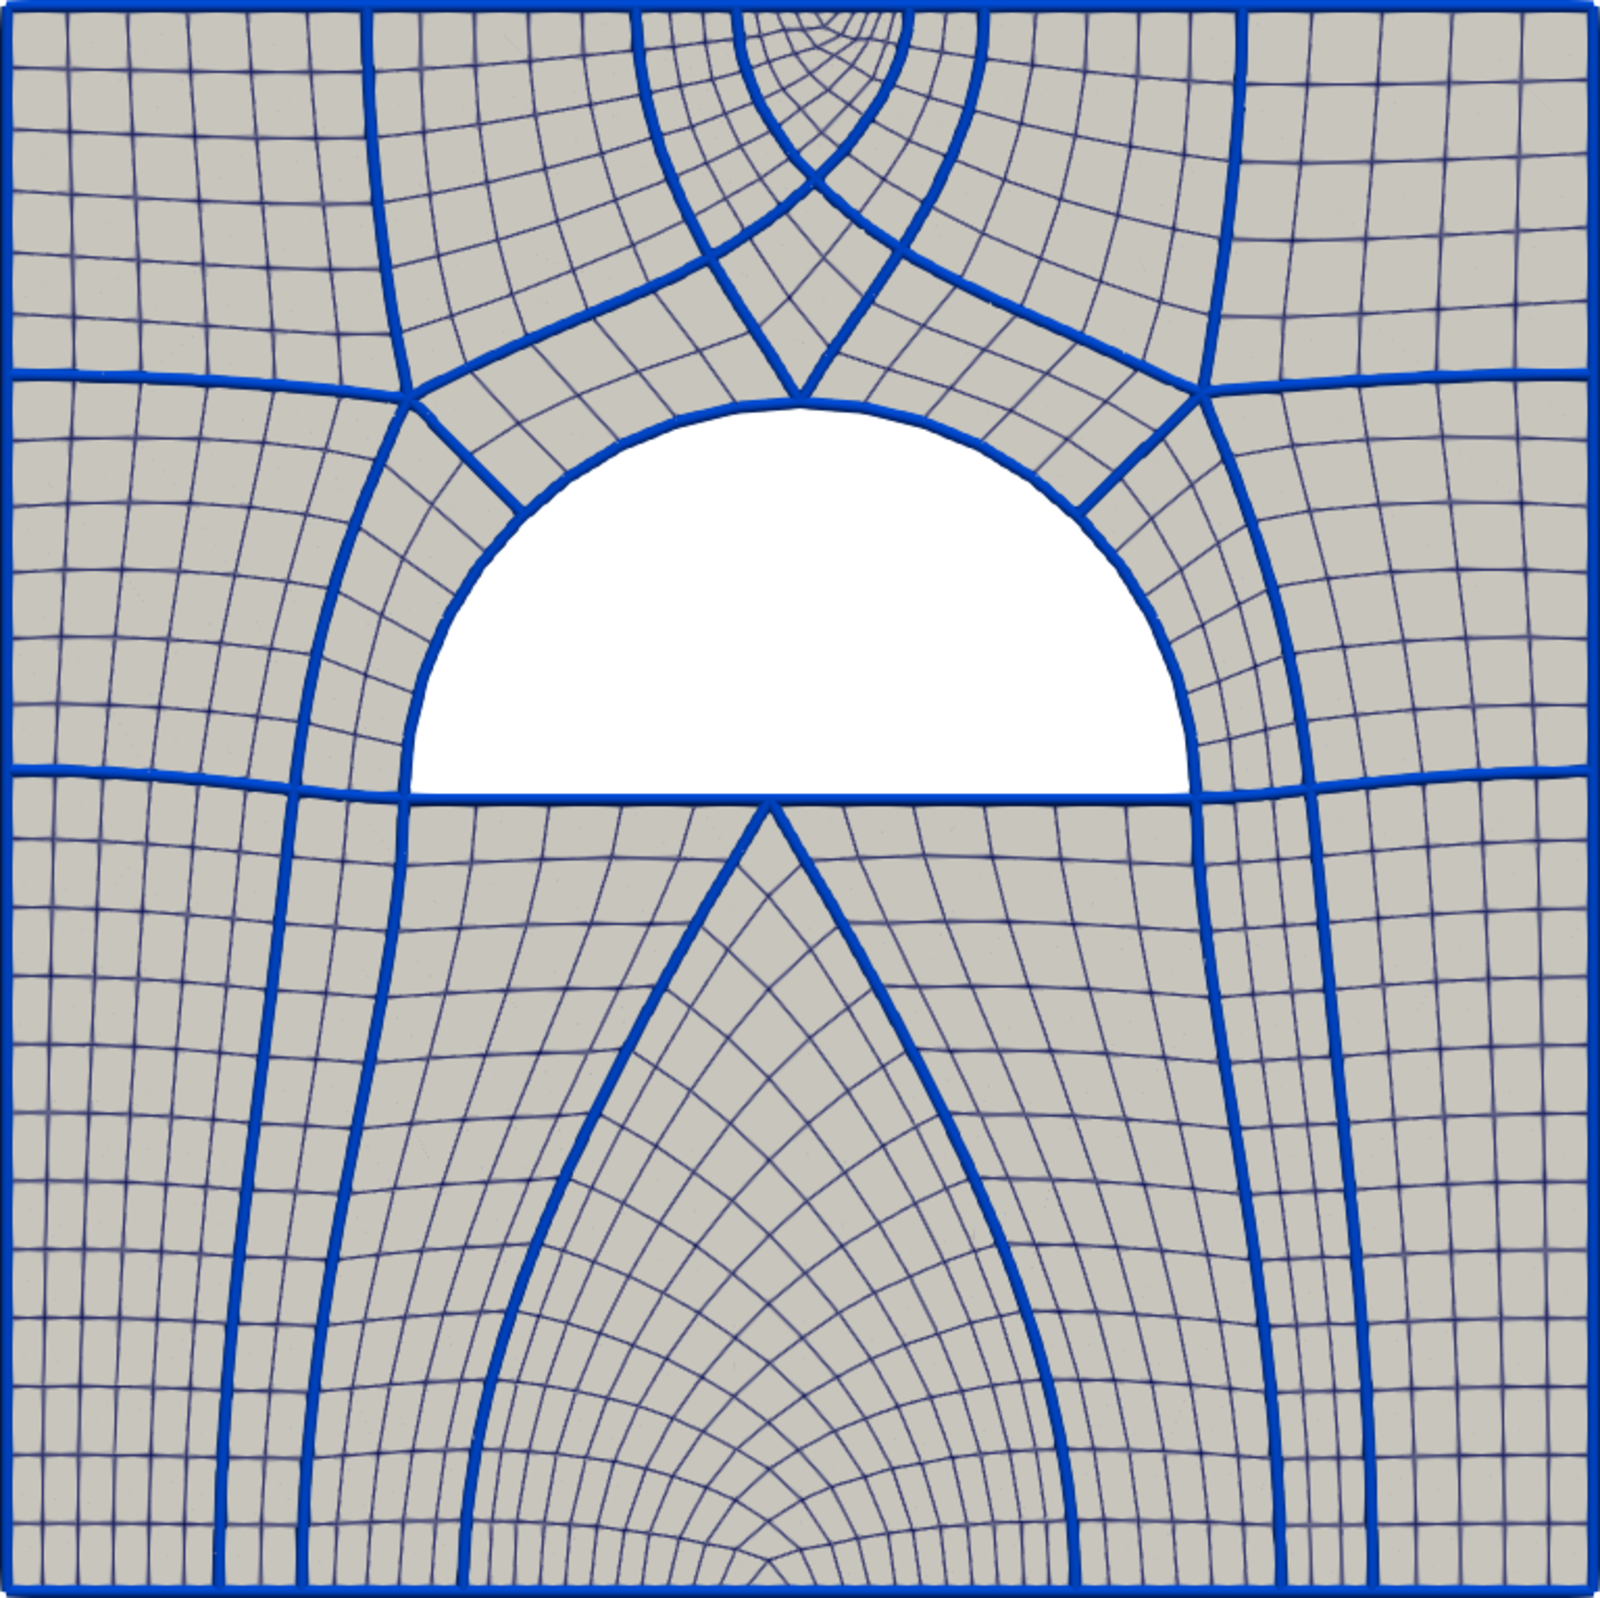
\includegraphics[width=\textwidth]{images/carre_demi_disc_vide_mauvais_third.pdf}
    \caption{Maillage quadilatéral du domaine présentant des quadrangles dégénérés.}
    \label{fig:carre_demi_disc_vide_mauvais_third}
\end{subfigure}
\caption{Illustration de l'opération d'alignement sur un domaine non-simplement connexe à partir d'un champ de croix vérifiant la condition \eqref{eqn:principe_hypothese_u_prime}.}
\label{fig:carre_demi_disc_vide_mauvais}
\end{figure}
Pour surmonter cette limitation, nous modifions la conditions à imposer sur le champ de croix initial $\bar{u}$ de la manière suivante:
\begin{equation}
    \left\{
    \begin{array}{lcll}
    \theta_{\bar{u}}^{\gamma_0}(1)-\theta_{\bar{u}}^{\gamma_0}(0)&=&2\pi-2\pi\displaystyle\sum_{p\in\mathcal{B}\cap\Gamma_0}I_p,&\mbox{ sur }\Gamma_0\\\\
    \theta_{\bar{u}}^{\gamma_i}(1)-\theta_{\bar{u}}^{\gamma_i}(0)&=&-2\pi-2\pi\displaystyle\sum_{p\in\mathcal{B}\cap\Gamma_i}I_p,&\mbox{ sur }\Gamma_i,~\forall i\in\llbracket 1, n_b-1\rrbracket.
    \end{array}
    \right.
    \label{eqn:principe_hypothese_u_second}
\end{equation}
où $\Gamma_0$ désigne le bord extérieur de $\Omega$. En supposant que le champ de croix $\bar{u}$ vérifie cette condition, la condition de bord de l'équation \eqref{eqn:principe_def_phi} devient:
$$
\phi(\gamma_i(t))=\theta_{\bar{N}}^{\gamma_i}(t)+\mathcal{I}(t)-\theta_{\bar{u}}^{\gamma_i}(t) \mbox{ sur } \gamma_i^{-1}(\Gamma_i\backslash(\mathcal{B}\cup\mathcal{S}_{\bar{u}})),~\forall i\in\llbracket 0, n_b-1\rrbracket.
$$
\begin{remark}
    On montre (voir le Théorème \ref{thm:theorem3}) que le champ de croix $\bar{v}$ (résultant de l'opération d'alignement) est aligné par rapport à $\partial\Omega$. De plus pour tout $p\in\Omega\backslash\partial\Omega$, $id_{\bar{v}}(p)=id_{\bar{u}}(p)$ et pour tout $p\in\partial\Omega$, $id_{\bar{v}}(p)=I_p$.
\end{remark}
La figure \ref{fig:carre_demi_disc_vide_bon} donne une illustration de la construction d'un maillage quadrilatéral sur un domaine non-simplement connexe à partir d'un champ de croix vérifiant la condition \ref{eqn:principe_hypothese_u_second}. La figure \ref{LS89} donne une représentation visuelle supplémentaire.

\begin{figure}[!h]
\centering
\begin{subfigure}{0.495\textwidth}
    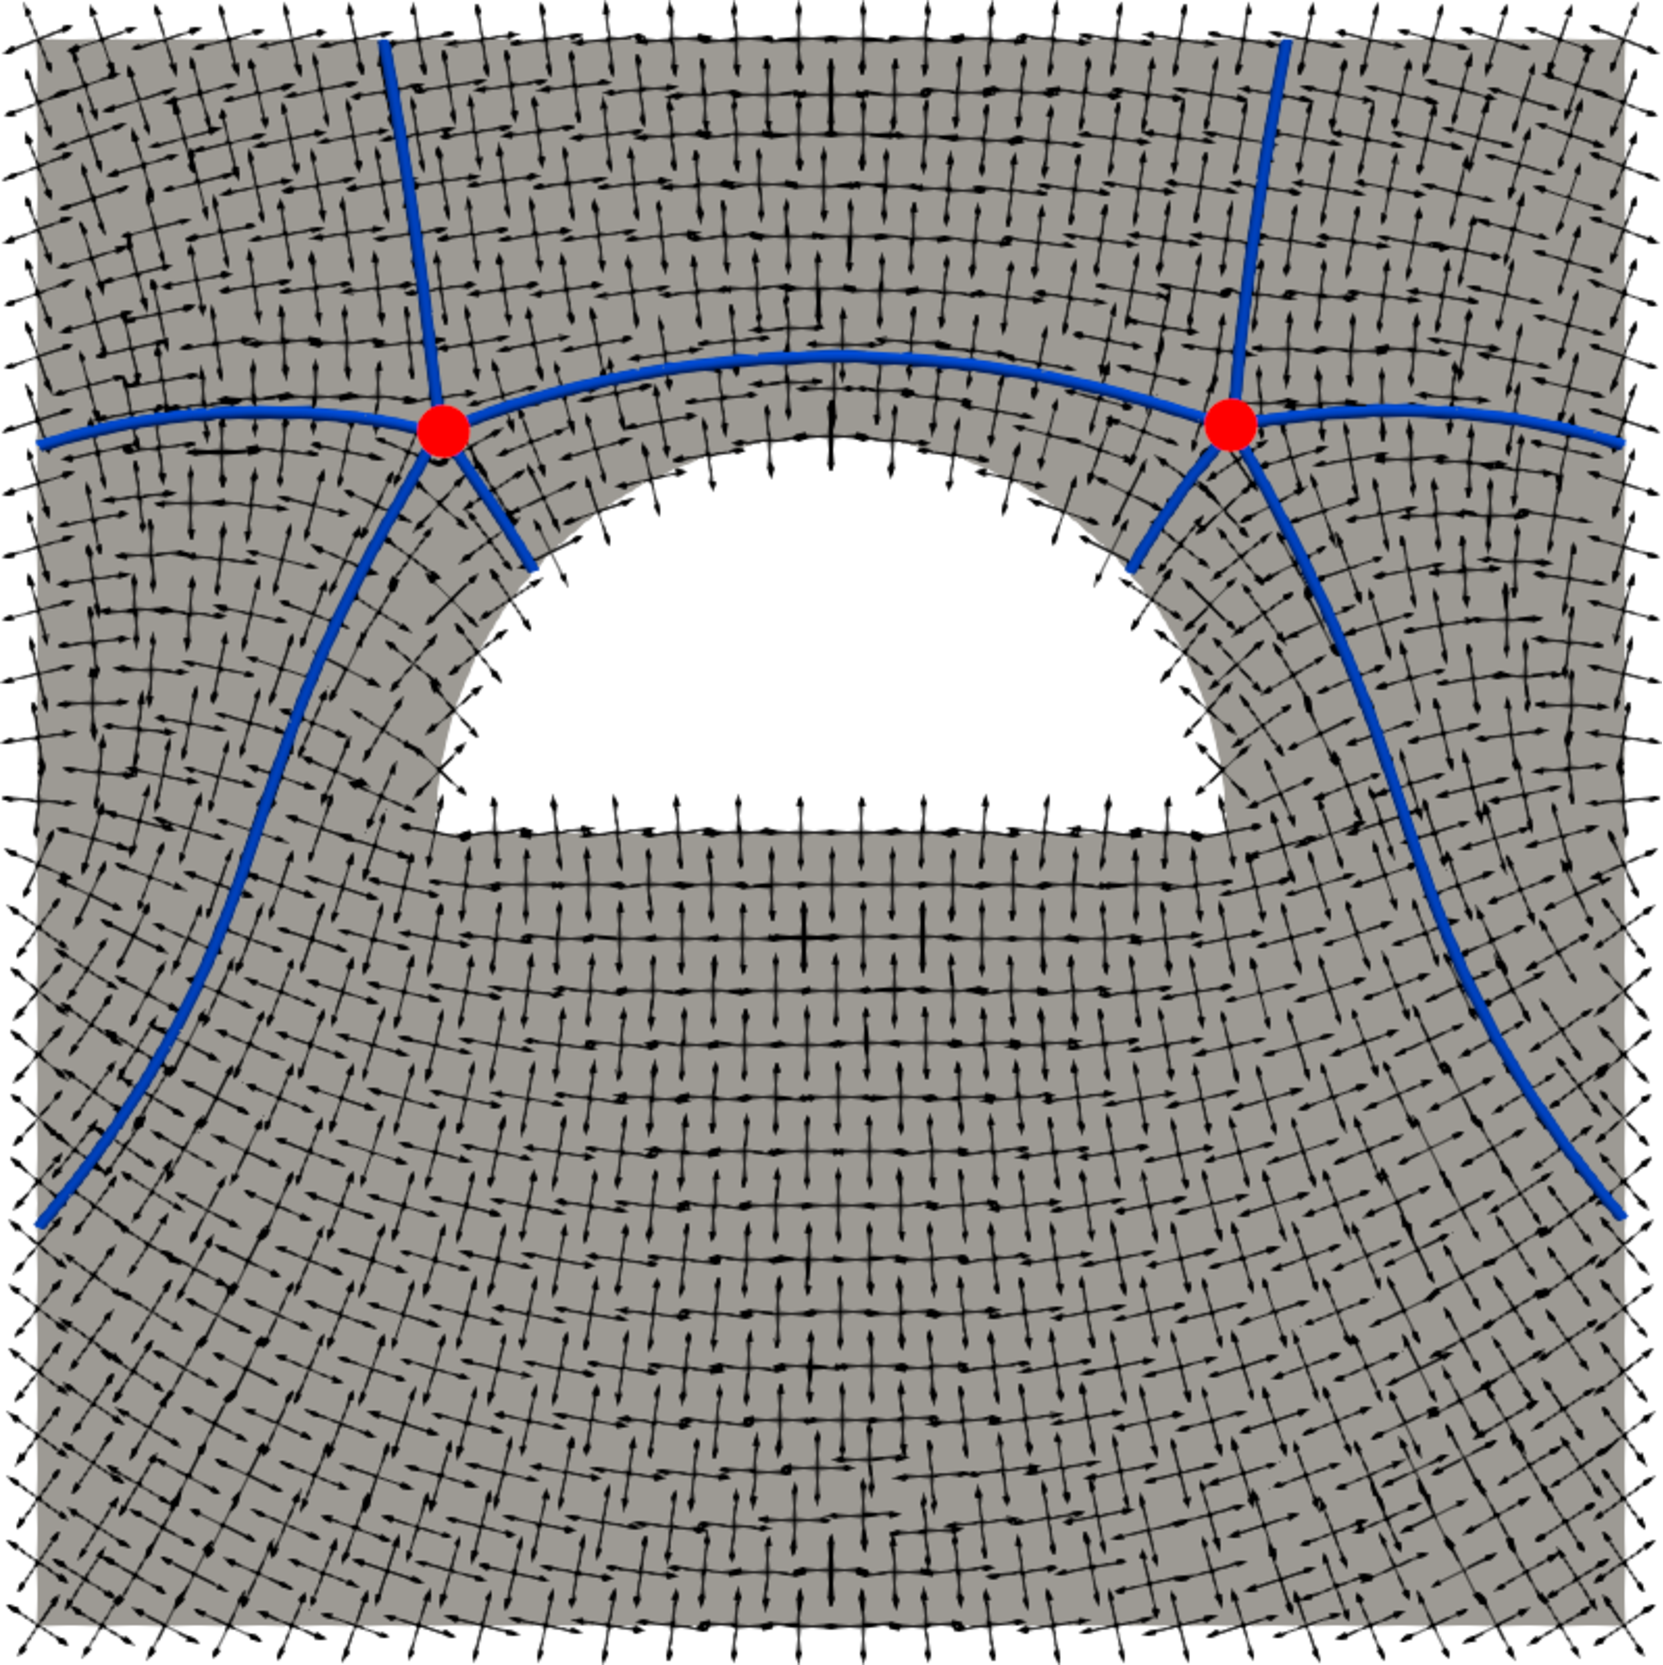
\includegraphics[width=\textwidth]{images/carre_demi_disc_vide_bon_first.pdf}
    \caption{Champ de croix initial avec deux points singuliers internes, chacun d'indice $1/4$ et vérifiant l'équation \ref{eqn:principe_hypothese_u_second}.}
    \label{fig:carre_demi_disc_vide_bon_first}
\end{subfigure}
\hfill
\begin{subfigure}{0.495\textwidth}
    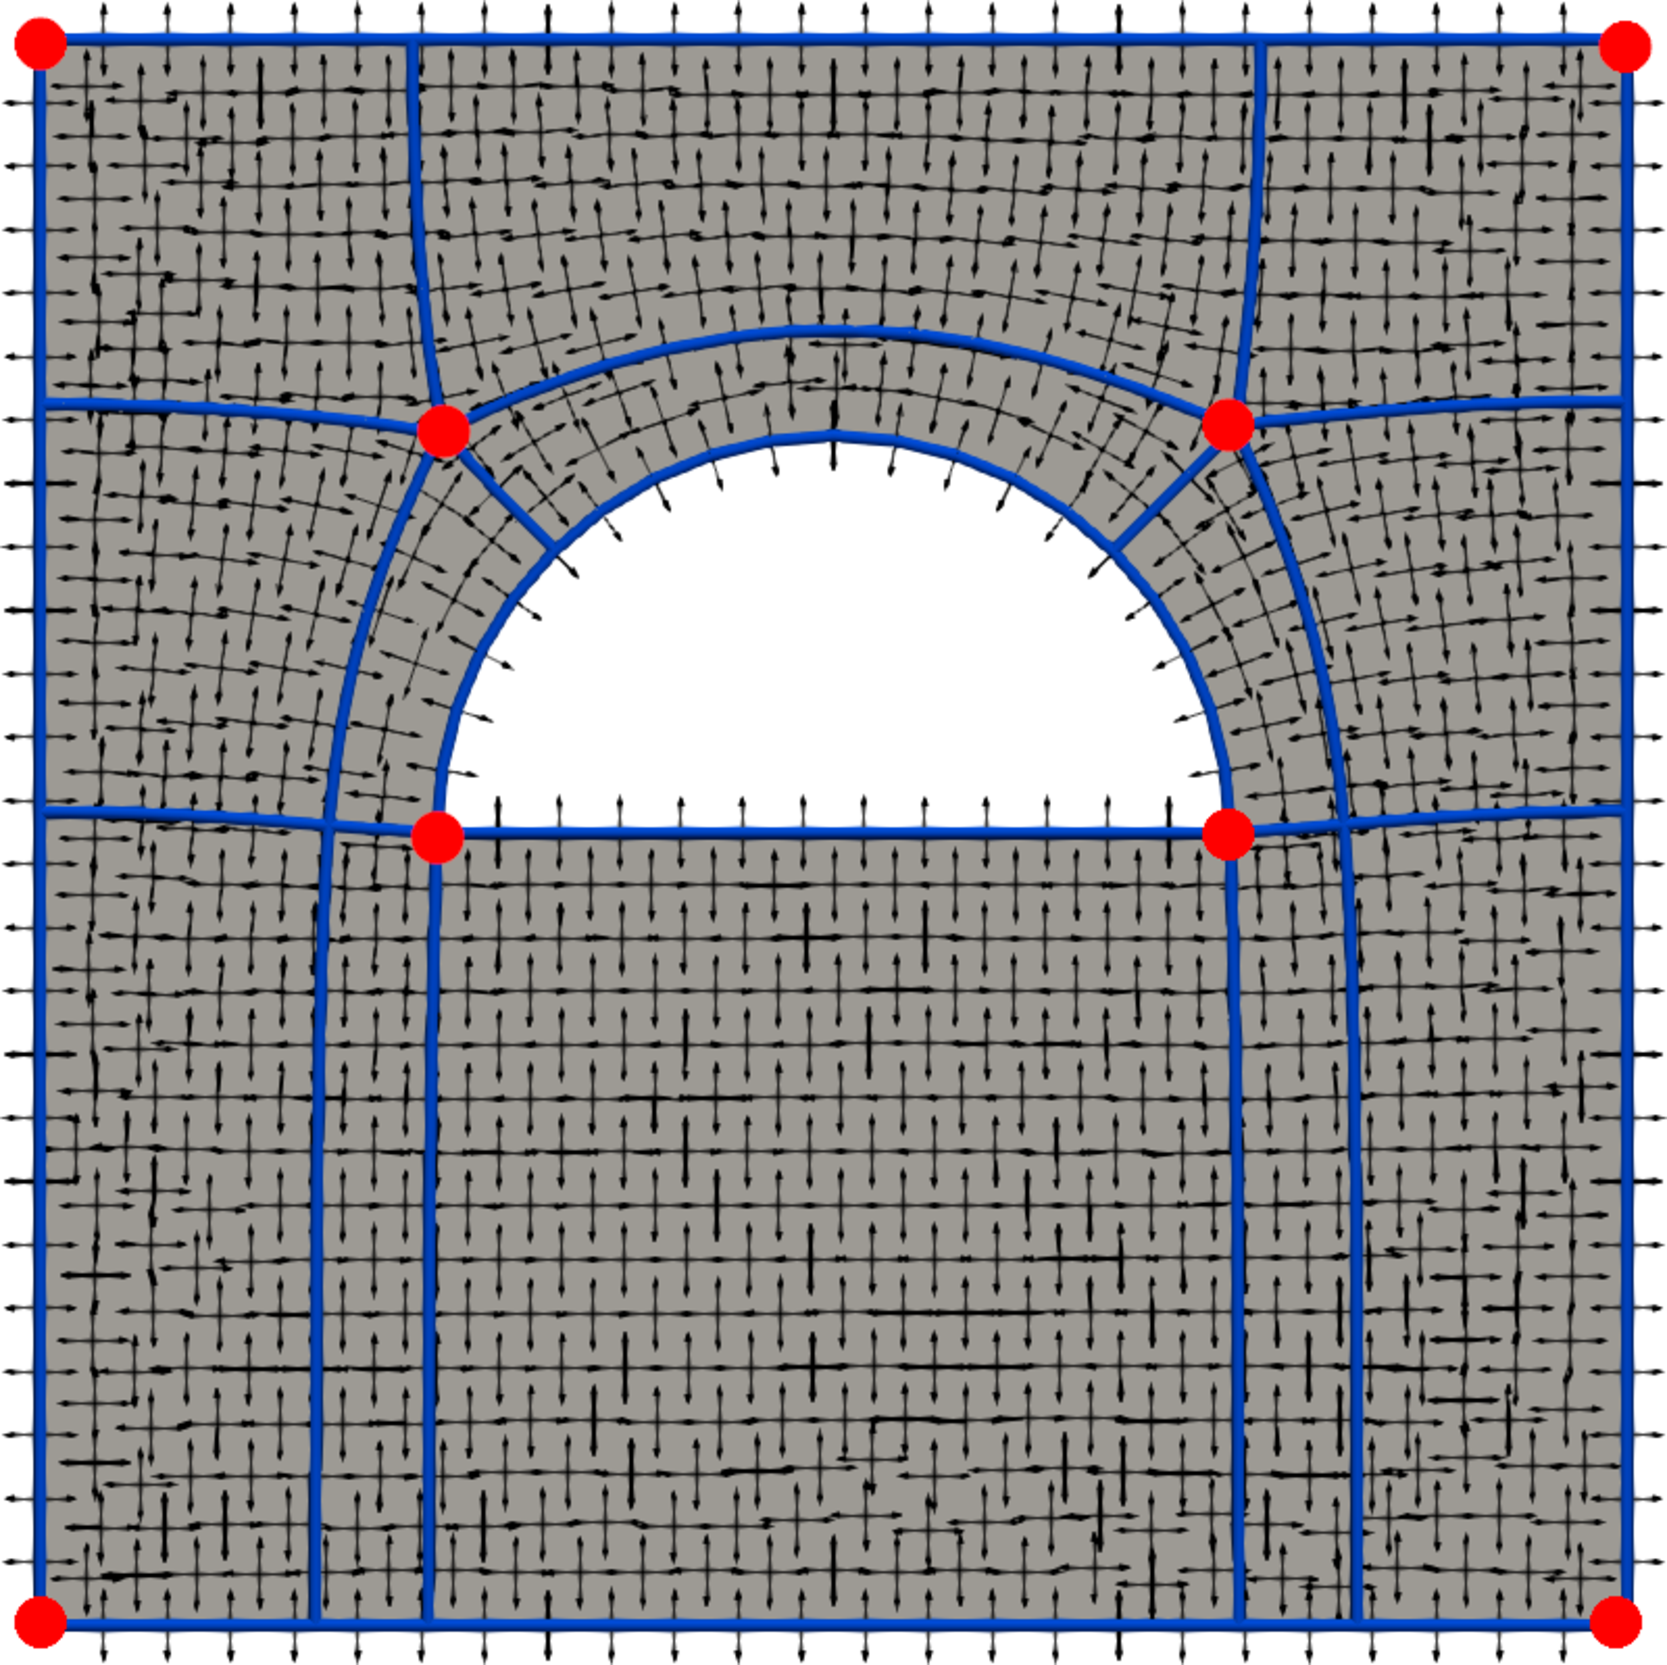
\includegraphics[width=\textwidth]{images/carre_demi_disc_vide_bon_second.pdf}
    \caption{Alignement du champ de croix initial sur le bord du domaine et partitionnement du domaine.}
    \label{fig:carre_demi_disc_vide_bon_second}
\end{subfigure}
\\[0.8cm]
\begin{subfigure}{0.5\textwidth}
    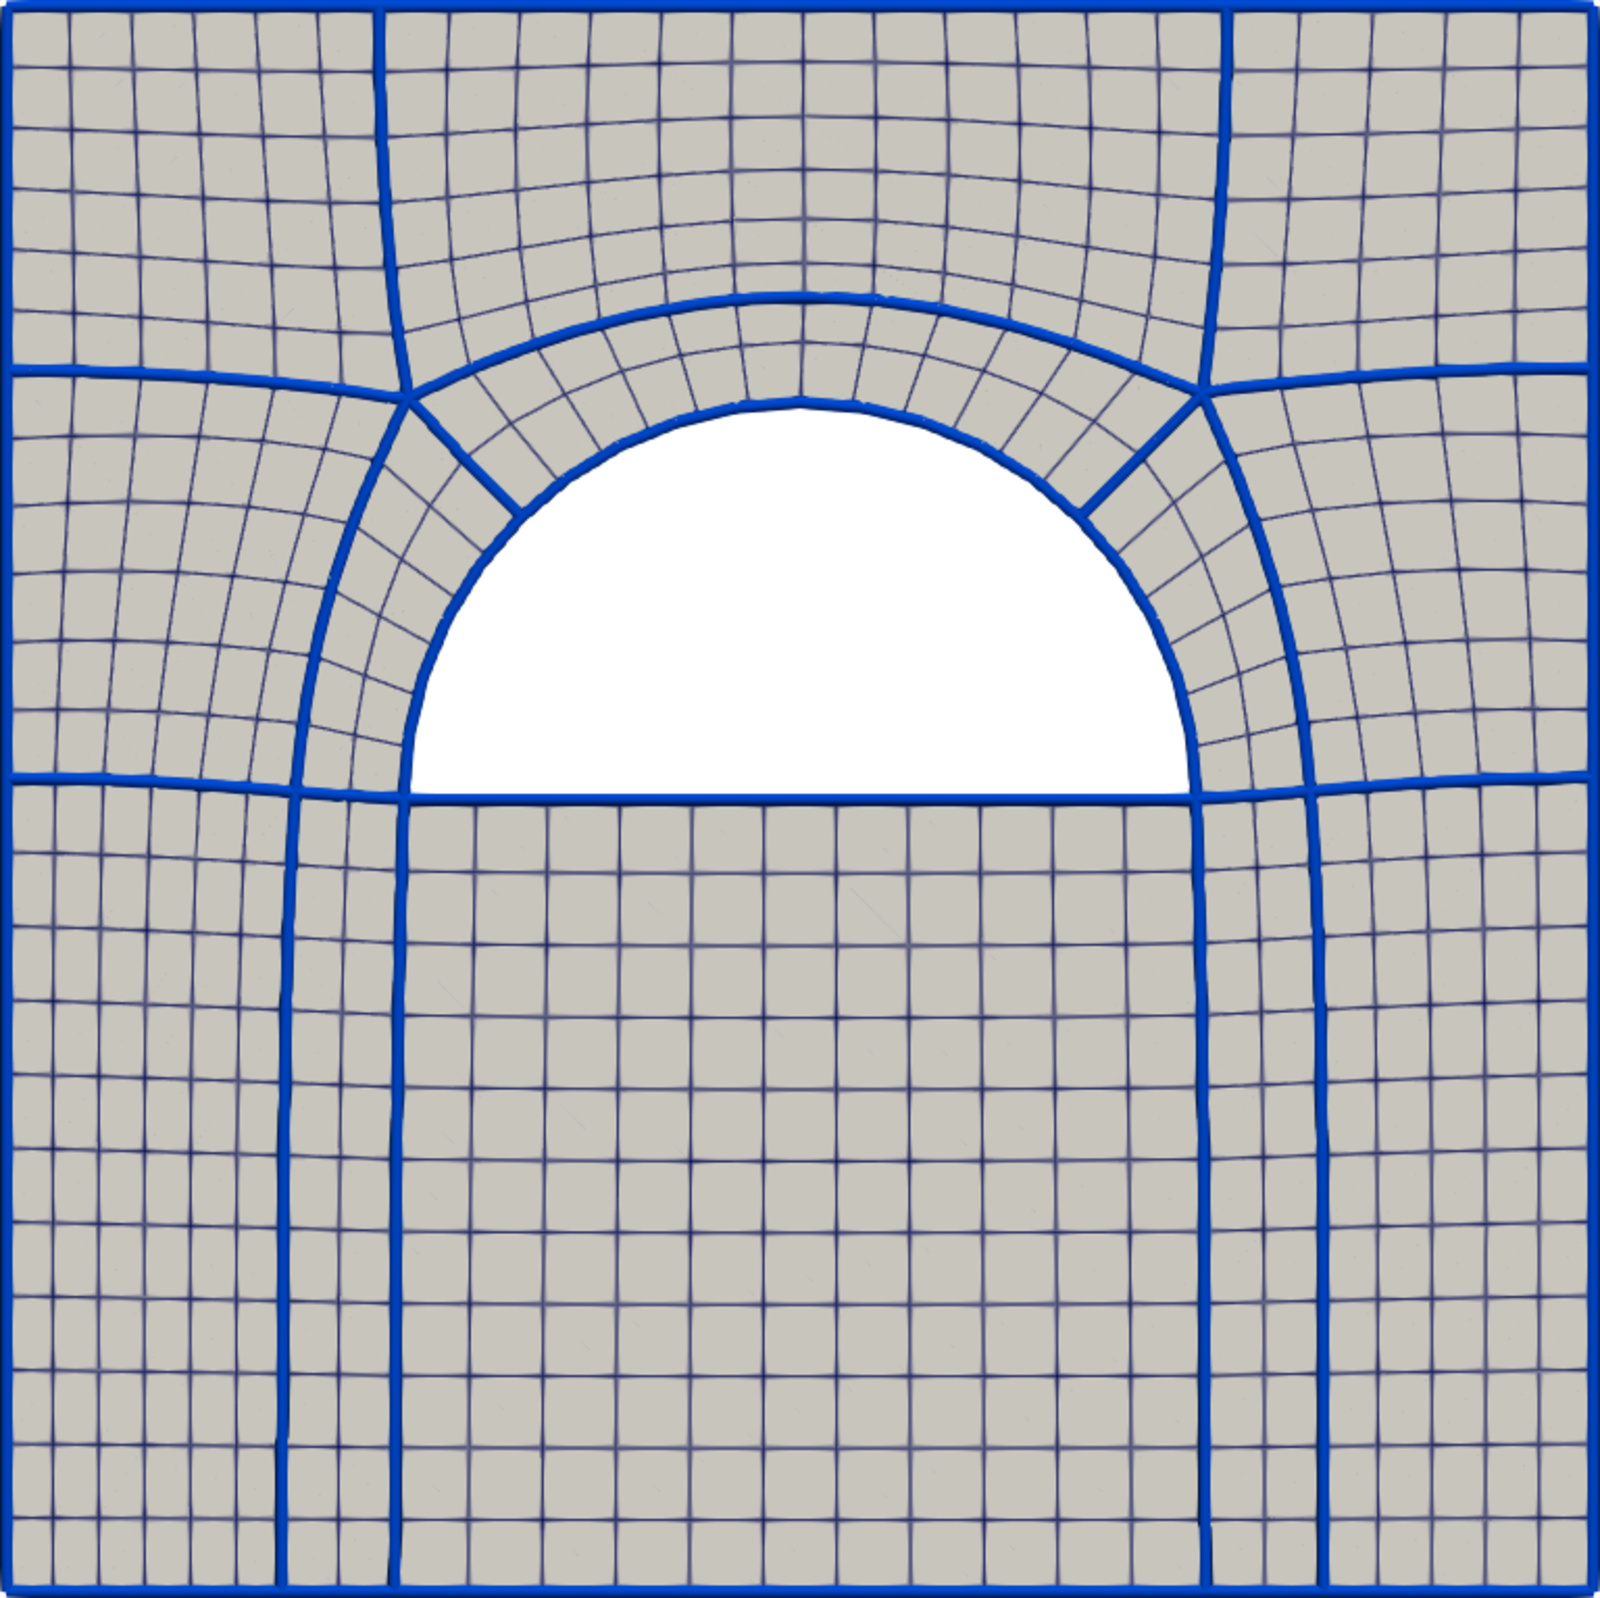
\includegraphics[width=\textwidth]{images/carre_demi_disc_vide_bon_third.pdf}
    \caption{Maillage quadilatéral du domaine.}
    \label{fig:carre_demi_disc_vide_bon_third}
\end{subfigure}
\caption{Illustration de l'opération d'alignement sur un domaine non-simplement connexe à partir d'un champ de croix vérifiant la condition \eqref{eqn:principe_hypothese_u_second}.}
\label{fig:carre_demi_disc_vide_bon}
\end{figure}

\paragraph{Correction d'un champ de croix ne vérifiant pas la condition \ref{eqn:principe_hypothese_u_second}:} D'après nos observations expérimentales, alors qu'il est relativement aisé de construire des champs de croix conformes à la formule \eqref{eqn:principe_hypothese_u_prime}, la génération de champs de croix respectant la formule \eqref{eqn:principe_hypothese_u_second} de manière simple et efficiente s'avère plus complexe. Par exemple le champ de croix illustré sur la figure \ref{fig:carre_demi_disc_vide_mauvais_first} vérifie \eqref{eqn:principe_hypothese_u_prime} mais pas \eqref{eqn:principe_hypothese_u_second}). Face à cette problématique, nous proposons une solution alternative en introduisant un processus de correction visant à modifier un champ de croix existant, $\bar{u}$ (vérifiant \ref{eqn:principe_hypothese_u_prime}), de manière à ce qu'il respecte la condition \eqref{eqn:principe_hypothese_u_second}. Cette démarche implique l'identification d'un champ d'angle $\omega$ permettant de définir un champ de croix corrigé, $\bar{u}_c$, à travers l'expression $\bar{u}_c:=\mathbf{R}(\omega)\bar{u}$, satisfaisant ainsi :
\begin{equation}
    \left\{
    \begin{array}{lcll}
    \theta_{\bar{u}_c}^{\gamma_0}(1)-\theta_{\bar{u}_c}^{\gamma_0}(0)&=&2\pi-2\pi\displaystyle\sum_{p\in\mathcal{B}\cap\Gamma_0}I_p,&\mbox{ sur }\Gamma_0\\\\
    \theta_{\bar{u}_c}^{\gamma_i}(1)-\theta_{\bar{u}_c}^{\gamma_i}(0)&=&-2\pi-2\pi\displaystyle\sum_{p\in\mathcal{B}\cap\Gamma_i}I_p,&\mbox{ sur }\Gamma_i,~\forall i\in\llbracket 1, n_b-1\rrbracket.
    \end{array}
    \right.
\end{equation}
De ce fait, le champ de croix corrigé $\bar{u}_c$ répond à la condition \eqref{eqn:principe_hypothese_u_second}. En appliquant le processus d'alignement à $\bar{u}_c$ ainsi que l'algorithme de partitionnement au champ résultant, nous parvenons à générer un maillage quadrilatéral du domaine initial. La construction du champ d'angle $\omega$ peut être effectuée selon diverses méthodes. Selon la méthode choisie, elle peut influencer les points singuliers de $\bar{u}$ et de l'ensemble $\mathcal{B}$ dans le maillage final. Nous reviendrons sur sa construction dans les parties suivantes (voir la section \ref{sec:discussion}).  L'algorithme \ref{alg:algo_non_simply_connected} résume la méthode de génération de maillage sur un domaine non-simplement connexe.

\vspace{0.5cm}
\begin{algorithm}[H]
\label{alg:algo_non_simply_connected}
\SetKwInOut{Input}{Entrée}
\SetKwInOut{Output}{Sortie}
\Input{$\Omega$ un domaine borné et fermé, champ de croix $\bar{u}$ défini sur $\Omega$, ensemble $\mathcal{B}$, paramètre $I(p)$ pour tout $p\in\partial\Omega$.}
\Output{Partition de $\Omega$ en ensembles de régions.}
\vspace{0.2cm}
1.) Correction du champ de croix si nécessaire,\\\vspace{0.2cm}
1.) Calcul du champ d'alignement,\\\vspace{0.2cm}
2.) Calcul du champ de croix $\bar{v}$,\\\vspace{0.2cm}
3.) Application de l'algorithme \ref{alg:algo_main} au champ de croix $\bar{v}$.\\\vspace{0.2cm}
\caption{Algorithme de partitionnement pour un domaine non-simplement connexe basé sur un champ de croix non aligné}
\end{algorithm}
\vspace{0.5cm}

\begin{figure}[!h]
\centering
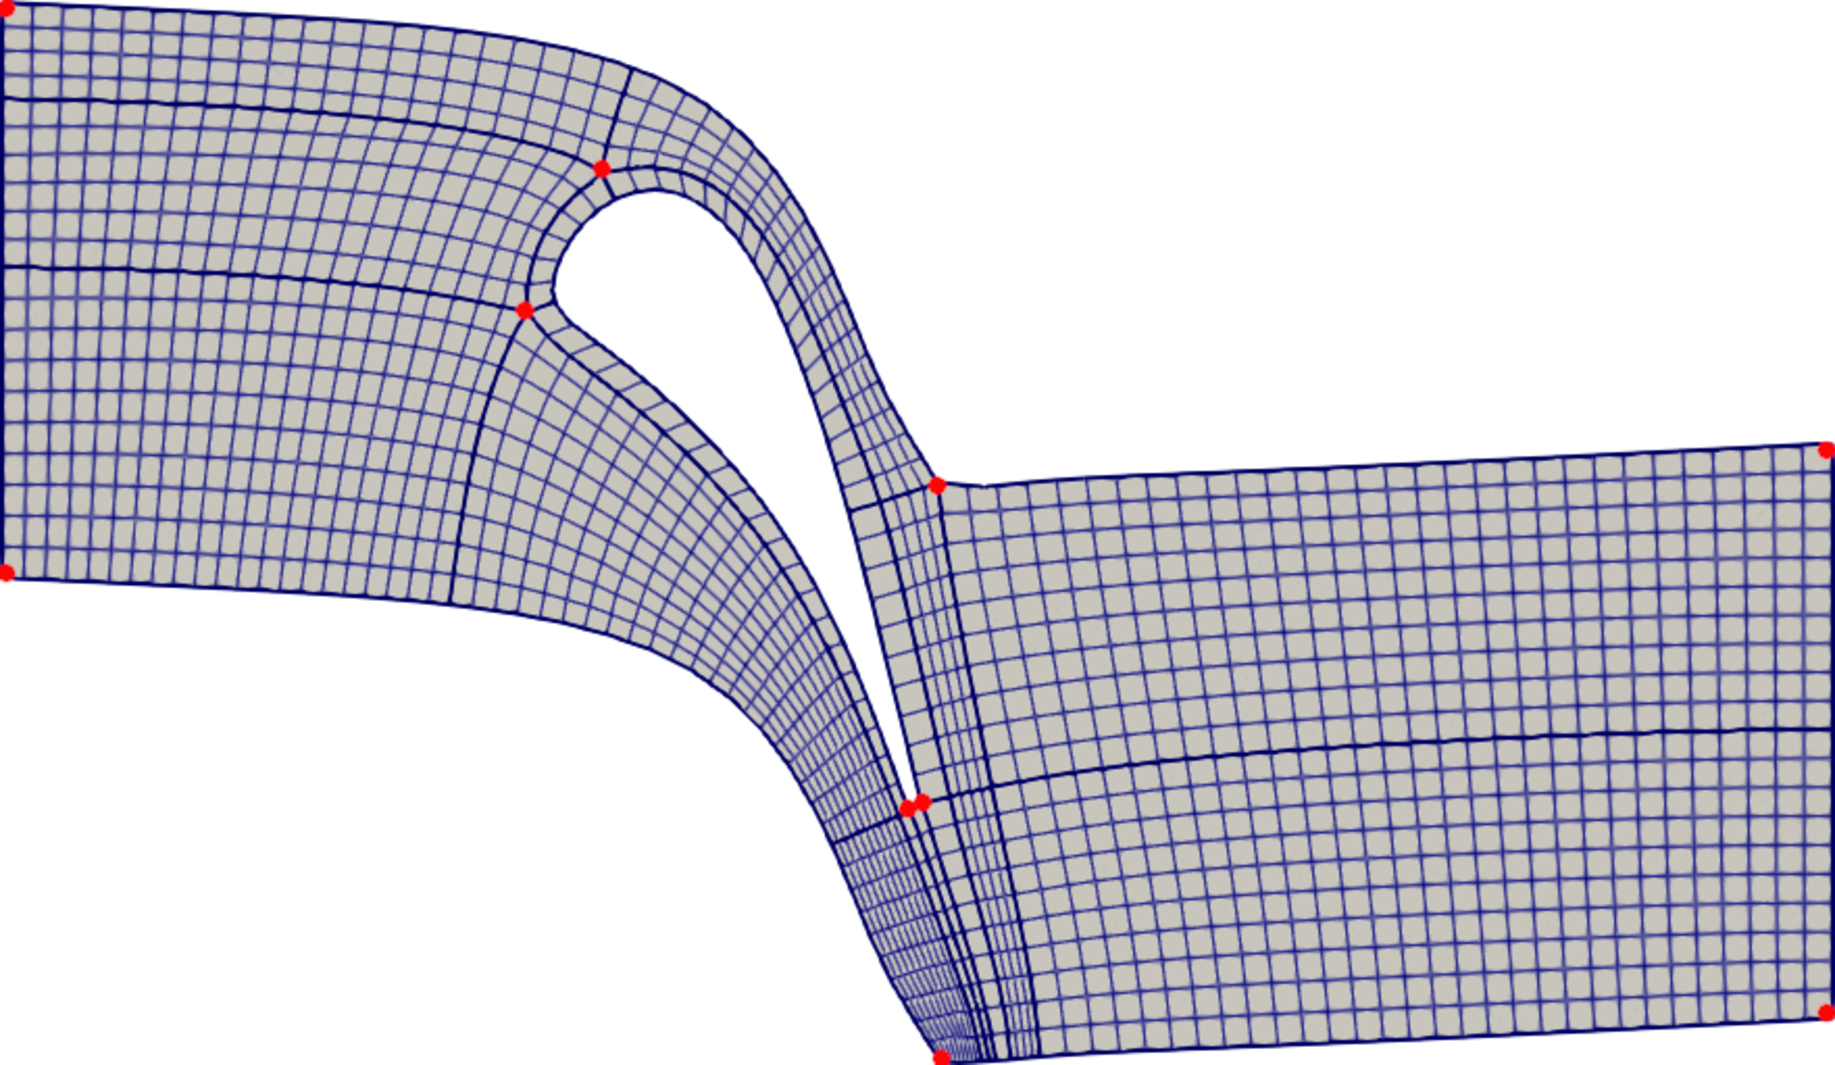
\includegraphics[scale=0.5]{images/LS89_bis.pdf}
\caption{Maillage du LS89 blade (géométrie détaillée dans \cite{gourdain2010advanced}).}
\label{LS89}
\end{figure}

\subsection{Etude de la méthode}
\label{subsec:etude_de_la_methode}
Dans la section précédente, nous avons exposé des algorithmes qui, sous certaines conditions, permettent de subdiviser un domaine en régions à quatres côtés. Dans cette partie, nous allons présenter plusieurs résultats visant à garantir l'efficacité de ces méthodes. Commençons par le cas où le champ de croix est aligné avec le bord du domaine. Nous avons le résultat suivant:
\begin{theorem}
\label{thm:theorem1}
Soit $\Omega$ un domaine borné et fermé dans $\mathbb{R}^2$ avec une frontière régulière par morceau et soit $\bar{u}$ un champ de croix presque-$\mathcal{C}^1$ aligné avec $\partial\Omega$ tel que $0<\#\mathcal{S}_{\bar{u}}<\infty$ et pour tout $p\in\Omega$, $id_{\bar{u}}(p)=k/4$ où $k\in\mathbb{Z}$ et $k\leq 1$. Si l'algorithme de partitionnement \ref{alg:algo_main} appliqué à $\bar{u}$ converge alors le partitionnement résultant est une décomposition de $\Omega$ en régions à quatre côtés.
\end{theorem}

\begin{proof}
Selon les propositions \ref{prop:stream_from_interior_sing} et \ref{prop:stream_from_bord_sing}, chaque point singulier de $u$ donne lieu à un nombre fini de séparatrices. Étant donné que ces séparatrices ne convergent pas vers des cycles limites, elles doivent soit se terminer en un point singulier, soit intersecter la frontière de $\Omega$. En conséquence, les séparatrices de $\bar{u}$ divisent $\Omega$ en régions qui ne contiennent aucun point singulier et qui sont délimitées par des séparatrices.

Soit $\mathcal{R}$ l'une de ces régions. Selon le Théorème de Poincaré-Hopf, on a $\chi(\mathcal{R})=\sum_{i=1}^{n_c} id_{\bar{u}}(c_i)$, où $(c_i)_{i\in\llbracket1,n_c\rrbracket}$ désigne les coins de $\mathcal{R}$ (c'est à dire les points d'intersections des séparatrices formant la région $\mathcal{R}$) et $n_c$ est le nombre de coins. $\chi(\mathcal{R})\geq0$ car, d'après la proposition \ref{prop:loveprop}, nous avons $id_{\bar{u}}(c_i)=1/4>0$ pour chaque coin $c_i$ de $\mathcal{R}$. De plus, on sait que $\chi(\mathcal{R}) = 2 - 2g - b$, où $g$ représente le genre de $\mathcal{R}$ et $b$ le nombre de composantes connexes de $\partial\mathcal{R}$. Comme $\mathcal{R}$ est une partie du plan, on a $g = 0$, ce qui implique que $\chi(\mathcal{R})\in\{0, 1\}$.
\begin{itemize}
\item $\chi(\mathcal{R})=0$: dans ce cas on a $n_c=0$ et $\mathcal{R}=\Omega$. Cela mène à une contradiction puisque, selon les hypothèses du théorème on a $\#\mathcal{S}_{\bar{u}}>0$.
\item $\chi(\mathcal{R})=1$: cela implique que :
$$1=\sum_{i=1}^{n_c}id_u(c_i)=\sum_{i=1}^{n_c}\frac{1}{4}\Longrightarrow n_c=4.$$
Ainsi, $\mathcal{R}$ est une région à quatre côtés.
\end{itemize}
\end{proof}

\paragraph{\'Etude de l'opération d'alignement}

Soit $\Omega$ un domaine fermé et borné dans $\mathbb{R}^2$ avec une frontière lisse par morceaux. Supposons dans un premier temps que $\Omega$ est simplement connexe. Soit $\mathcal{B}\subset\partial\Omega$ un ensemble de point isolé de $\partial\Omega$ et $I_p$ un paramètre associé à chaque point $p\in\Omega$ tel que:
\begin{equation}
I_p=
\left\{
\begin{array}{ll}
\displaystyle\frac{k}{4}\mbox{ avec }k\in\mathbb{Z}\mbox{ et }k\leq 1& \mbox{ si } p\in\mathcal{B}\\[0.5cm]
0& \mbox{ sinon }
\end{array}
\right.
\label{eqn:etude_def_I}
\end{equation}
Soit $\bar{u}$ un champ de croix presque-$\mathcal{C}^1$ défini sur $\Omega$, non nécessairement aligné sur $\partial\Omega$, tel que $0<\#\mathcal{S}_{\bar{u}}<\infty$ et pour tout point $p\in\mathcal{S}_{\bar{u}}\backslash\partial\Omega$, $id_{\bar{u}}(p)=k/4$, avec $k\in\mathbb{Z}$ et $k\leq 1$. On suppose de plus qu'il existe $\theta_{\bar{u}}^\gamma$ un relèvement continu de $\bar{u}$ le long de $\gamma$ tel que:
\begin{equation}
    \label{eqn:etude_hypothese_u}
    \theta_{\bar{u}}^\gamma(1)-\theta_{\bar{u}}^\gamma(0)=2\pi\chi(\Omega)-2\pi\sum_{p\in\mathcal{B}}I_p.
\end{equation}
où $\gamma$ est une paramétrisation sur $[0, 1]$ de $\partial\Omega$ orientée positivement et vérifiant $\gamma(0)=\gamma(1)\notin\mathcal{B}\cup\mathcal{S}_{\bar{N}}\cup\mathcal{S}_{\bar{u}}$.
Soit $\phi$, la fonction définie par l'équation de Laplace suivant:
\begin{equation}
\left\{
\begin{array}{lcll}
\Delta\phi &=& 0 &\mbox{ dans }\Omega,\\[0.5cm]
\phi(\gamma(t))&=&\theta_{\bar{N}}^\gamma(t)+\mathcal{I}(t)-\theta_{\bar{u}}(\gamma(t))& \mbox{ sur } \gamma^{-1}(\partial\Omega\backslash(\mathcal{B}\cup\mathcal{S}_{\bar{N}}\cup\mathcal{S}_{\bar{u}})),
\end{array}
\right.
\label{eqn:etude_def_phi}
\end{equation}
où la fonction $\mathcal{I}$ est donnée pour tout $t\in\gamma^{-1}(\partial\Omega\backslash(\mathcal{B}\cup\mathcal{S}_{\bar{N}}\cup\mathcal{S}_{\bar{u}}))$ par:
$$
\mathcal{I}(t)=\sum_{s\in\gamma^{-1}(\mathcal{B}\cup\mathcal{S}_{\bar{N}})}\left[\left(\pi-\widehat{\gamma(s)}-2\pi I_{\gamma(s)}\right)-\left(\lim\limits_{r\rightarrow s^+}\theta^{\gamma}_{\bar{N}}(r) - \lim\limits_{r\rightarrow s^-}\theta^{\gamma}_{\bar{N}}(r)\right)\right]\mathbb{1}_{[0, t]}(s),
$$
avec $\widehat{\gamma(s)}$ la mesure de l'ouverture angulaire de la frontière en $\gamma(s)$. Nous avons alors le lemme suivant:

\begin{lemma}
    \label{lem:marvelous_lemma}
    $\phi(\gamma(1))-\phi(\gamma(0))=0$.
\end{lemma}
\begin{proof}
    $$
    \begin{array}{lcl}
        \phi(\gamma(1))-\phi(\gamma(0))&=&\theta^\gamma_{\bar{N}}(1)+\mathcal{I}(1)-\theta_{\bar{u}}(\gamma(1))-(\theta^\gamma_{\bar{N}}(0)+\mathcal{I}(0)-\theta_{\bar{u}}(\gamma(0)))\\\\
        &=&(\theta^\gamma_{\bar{N}}(1)-\theta_{\bar{N}}^\gamma(0))+(\mathcal{I}(1)-\mathcal{I}(0))-(\theta_{\bar{u}}(\gamma(1))-\theta_{\bar{u}}(\gamma(0))
    \end{array}
    $$
    En posant $\gamma^{-1}(\mathcal{B}\cup\mathcal{S}_{\bar{N}})=\{t_1,\dots,t_{n_t}\}$ avec $n_t\in\mathbb{N}^*$ et $t_1<\dots<t_{n_t}$, on a:
    $$
    \begin{array}{lcl}
        \theta_{\bar{N}}^\gamma(1)-\theta^\gamma_{\bar{N}}(0)&=&\theta_{\bar{N}}^\gamma(t_1^-)-\theta_{\bar{N}}^\gamma(0)+\displaystyle\sum_{i=2}^{n_t}\left(\theta_{\bar{N}}^\gamma(t_i^-)-\theta_{\bar{N}}^\gamma(t_{i-1}^+)\right)+\theta_{\bar{N}}^\gamma(0)\\[0.7cm]
        &&+\theta_{\bar{N}}^\gamma(1)-\theta_{\bar{N}}^\gamma(t_{n_t}^-)+\displaystyle\sum_{i=1}^{n_t}\left(\theta_{\bar{N}}^\gamma(t_i^+)-\theta_{\bar{N}}^\gamma(t_i^-)\right)-\theta_{\bar{N}}^\gamma(0)\\[0.7cm]
        &=&\displaystyle\int_0^1d\theta_{\bar{N}}^\gamma+\displaystyle\sum_{i=1}^{n_t}\left(\theta_{\bar{N}}^\gamma(t_i^+)-\theta_{\bar{N}}^\gamma(t_i^-)\right)\\[0.7cm]
        \theta_{\bar{N}}^\gamma(1)-\theta^\gamma_{\bar{N}}(0)&=&\displaystyle\int_0^1d\theta_{\bar{N}}^\gamma+\displaystyle\sum_{s\in\gamma^{-1}(\mathcal{B}\cup\mathcal{S}_{\bar{N}})}\left(\theta_{\bar{N}}^\gamma(s^+)-\theta_{\bar{N}}^\gamma(s^-)\right)
    \end{array}
    $$
    Remarquons aussi que puisque $\mathcal{I}(0)=0$, on a:
    $$
    \mathcal{I}(1)-\mathcal{I}(0)=\sum_{s\in\gamma^{-1}(\mathcal{B}\cup\mathcal{S}_{\bar{N}})}\left[\left(\pi-\widehat{\gamma(s)}-2\pi I_{\gamma(s)}\right)-\left(\theta^{\gamma}_{\bar{N}}(s^+)-\theta^{\gamma}_{\bar{N}}(s^-)\right)\right].
    $$
    Il vient alors que:
    $$
    \phi(\gamma(1))-\phi(\gamma(0))=\displaystyle\int_0^1d\theta_{\bar{N}}^\gamma+\sum_{s\in\gamma^{-1}(\mathcal{B}\cup\mathcal{S}_{\bar{N}})}\left(\pi-\widehat{\gamma(s)}-2\pi I_{\gamma(s)}\right)-(\theta_{\bar{u}}^\gamma(1)-\theta_{\bar{u}}^\gamma(0)).
    $$
    Autrement dit,
    $$
    \begin{array}{lcl}
        \phi(\gamma(1))-\phi(\gamma(0))&=&\displaystyle\sum_{i=1}^{n_t}\int_{t_i}^{t_{i+1}}d\theta_{\bar{N}}^\gamma+\sum_{s\in\gamma^{-1}(\mathcal{B})}\left(\pi-\widehat{\gamma(s)}\right)\\[0.7cm]
        &&-\displaystyle\left(\sum_{s\in\gamma^{-1}(\mathcal{B}\cup\mathcal{S}_{\bar{N}})}2\pi I_{\gamma(s)}+(\theta_{\bar{u}}^\gamma(1)-\theta_{\bar{u}}^\gamma(0))\right)
    \end{array}
    $$
    où on a posé $t_{n_t+1}:=t_1$. D'après le théorème des tangentes tournantes \cite{hopf1935drehung, rotskoff2010gauss}, on sait que :
    $$
    \displaystyle\sum_{i=1}^{n_t}\left(\theta_{\bar{N}}^\gamma(t_{i+1})-\theta_{\bar{N}}^\gamma(t_i)\right)+\sum_{s\in\gamma^{-1}(\mathcal{B}\cup\mathcal{S}_{\bar{N}})}\left(\pi-\widehat{\gamma(s)}\right)=2\pi.
    $$
    On obtient alors en utilisant la condition \eqref{eqn:etude_hypothese_u}
    $$
    \phi(\gamma(1))-\phi(\gamma(0))=2\pi-2\pi\chi(\Omega).
    $$
    Autrement dit,
    $$
    \phi(\gamma(1))-\phi(\gamma(0))=0.
    $$
\end{proof}
L'opération d'alignement consiste à calculer le champ de croix $\bar{v}$ défini pour tout $p\in\Omega$ par:
\begin{equation}
\bar{v}(p)=
\left\{
\begin{array}{ll}
\mathbf{R}(\phi(p))\bar{u}(p) & \mbox{ si } p\in\Omega\backslash(\mathcal{B}\cup\mathcal{S}_{\bar{N}}\cup\mathcal{S}_{\bar{u}}),\\[0.5cm]
\bar{N}(p) & \mbox{ si } p\in(\mathcal{S}_{\bar{u}}\cap\partial\Omega)\backslash(\mathcal{B}\cup\mathcal{S}_{\bar{N}}),\\[0.5cm]
0 & \mbox{ si } p\in\mathcal{B}\cup\mathcal{S}_{\bar{N}}.
\end{array}
\right.
\label{eqn:etude_def_v}
\end{equation}
Nous avons alors le théorème suivant:
\begin{theorem}
\label{thm:theorem2}
Le champ de croix $\bar{v}$ est presque-$\mathcal{C}^1$ sur $\Omega$ et aligné avec $\partial\Omega$. De plus, pour tout $p\in\Omega$, on a:
\begin{equation}
id_{\bar{v}}(p)=
\left\{
\begin{array}{ll}
    id_{\bar{u}}(p) & \mbox{ si } p\in\Omega\backslash\partial\Omega,\\\\
    I_p & \mbox{ sinon }.
\end{array}
\right.
\end{equation}
\end{theorem}

\begin{proof}
    Du fait que la fonction $\phi$ définie par l'équation \eqref{eqn:etude_def_phi} est de classe $\mathcal{C}^1$ sur $\Omega\backslash(\mathcal{B}\cup\mathcal{S}_{\bar{N}}\cup(\mathcal{S}_{\bar{u}}\cap\partial\Omega)))$, le champ $\bar{v}$ est presque-$\mathcal{C}^1$ sur $\Omega$. Cela découle immédiatement de la proposition \ref{prop:cont1}, étant donné que $\bar{u}$ est presque-$\mathcal{C}^1$ sur $\Omega$.

    De plus, $\bar{v}$ est aligné avec $\partial\Omega$. En effet, $\bar{v}(p)=0$ pour tout $p\in\mathcal{B}\cup\mathcal{S}_{\bar{N}}$ et $\bar{v}(p)=\bar{N}(p)$ pour tout $p\in(\mathcal{S}_{\bar{u}}\cap\partial\Omega)\backslash(\mathcal{B}\cup\mathcal{S}_{\bar{N}})$. Par ailleurs, pour tout $p\in\partial\Omega\backslash(\mathcal{B}\cup\mathcal{S}_{\bar{N}}\cup\mathcal{S}_{\bar{u}})$ on a:
    $$\theta_{\bar{v}}(\gamma(t_p))=\phi(\gamma(t_p))+\theta_{\bar{u}}^\gamma(t_p)+k\frac{\pi}{2}=\theta_{\bar{N}}^\gamma(t_p)+\mathcal{I}(t_p)-\theta_{\bar{u}}^\gamma(t_p)+\theta_{\bar{u}}^\gamma(t_p)+k\frac{\pi}{2},$$
    où $t_p\in[0,1]$ tel que $\gamma(t_p)=p$ et $k\in\mathbb{Z}$. Or pour tout $s\in\gamma^{-1}(\mathcal{B}\cup\mathcal{S}_{\bar{N}})\cap[0, t_p]$ on a:
    $$
    \lim\limits_{r\rightarrow s^+}\theta^{\gamma}_{\bar{N}}(r) - \lim\limits_{r\rightarrow s^-}\theta^{\gamma}_{\bar{N}}(r)\equiv(\pi-\widehat{\gamma(s)})\pmod{\frac{\pi}{2}}.
    $$
    Il vient alors que:
    $$
    \theta_{\bar{v}}(\gamma(t_p))=\theta_{\bar{N}}^{\gamma}(t_p)+\displaystyle\sum_{s\in\gamma^{-1}(\mathcal{B}\cup\mathcal{S}_{\bar{N}})}\left[\left(\pi-\widehat{\gamma(s)}-m_s\frac{\pi}{2}\right)-\left(\pi-\widehat{\gamma(s)}+k_s\frac{\pi}{2}\right)\right]\mathbb{1}_{[0, t_p]}(s)+k\frac{\pi}{2},
    $$
    où $k_s\in\mathbb{Z}$ et où on a posé $I_{\gamma(s)}=m_s/4$ avec $m_s\in\mathbb{Z}$ et $m_s\leq1$. Autrement dit, on a:
    $$
    \theta_{\bar{v}}(\gamma(t_p))=\theta_{\bar{N}}^\gamma(t_p)+\displaystyle\sum_{s\in\gamma^{-1}(\mathcal{B}\cup\mathcal{S}_{\bar{N}})}\left[-m_s\frac{\pi}{2}+k_s\frac{\pi}{2}\right]\mathbb{1}_{[0, t_p]}(s)+k\frac{\pi}{2}$$
    et donc:
    $$
    \theta_{\bar{v}}(\gamma(t_p))\equiv\theta_{\bar{N}}^\gamma(t_p)\pmod{\frac{\pi}{2}}.
    $$
    Ce qui implique que $\bar{v}(p)=\bar{N}(p)$. On conclut alors que $\bar{v}$ est aligné avec $\partial\Omega$.\\\\
    Nous calculons maintenant pour tout $p\in\Omega$, l'indice de $p$ dans le champ $\bar{v}$. Ainsi, on a:\\
    \begin{itemize}
        \item[$\bullet$] Si $p\in\Omega\backslash\partial\Omega$, $id_{\bar{v}}(p)=id_{\bar{u}}(p)$ selon la proposition \ref{prop:relation_u_Rthetau}, car la fonction $\phi$ définie par l'équation \eqref{eqn:etude_def_phi} est de classe $\mathcal{C}^1$ sur $\Omega\backslash\partial\Omega$.\\
        \item[$\bullet$] Si $p\in\partial\Omega\backslash\{\gamma(0)\}$ (sachant que $\gamma(0)=\gamma(1)$), on a:
        $$
        id^\partial_{\bar{v}}(p)=\frac{1}{2\pi}\left[\pi-\widehat{p}+\displaystyle\lim\limits_{s\rightarrow 0}\int_s^{1-s}d\theta_{\bar{v}}^{\mathcal{C}}\right]=\frac{1}{2\pi}\left(\pi-\widehat{p}+(\theta_{\bar{v}}^{\mathcal{C}}(1)-\theta_{\bar{v}}^{\mathcal{C}}(0))\right),
        $$
        où $\mathcal{C}$ est un lacet paramétré sur $[0, 1]$ tel que $\mathcal{C}(0)=p=\mathcal{C}(1)$ et les vecteurs $\mathcal{C}'(0)$ et $\mathcal{C}'(1)$ sont tangents à $\partial\Omega$. De plus, $\mathcal{C}$ n'englobe aucun autre point singulier de $\bar{u}$. Soit $t_p\in]0, 1[$ tel que $\gamma(t_p)=p$. On a:
        $$
        id^\partial_{\bar{v}}(p)=\frac{1}{2\pi}\left[\pi-\widehat{p}+\left(\theta_{\bar{v}}^\gamma(t_p^-)-\theta_{\bar{v}}^\gamma(t_p^+)\right)\right]
        $$
        où on a noté $\lim_{t\rightarrow t_p^+}\theta^\gamma_{\bar{v}}(t)=\theta^\gamma_{\bar{v}}(t_p^+)$ et $\lim_{t\rightarrow t_p^-}\theta^\gamma_{\bar{v}}(t)=\theta_{\bar{v}}^\gamma(t_p^-)$. Autrement dit, on a:
        $$
        \begin{array}{lcl}
        id^\partial_{\bar{v}}(p)&=&\displaystyle\frac{1}{2\pi}\left[\pi-\widehat{p}+\left(\phi(\gamma(t_p^-))+\theta_{\bar{u}}^\gamma(t_p^-)-\phi(\gamma(t_p^+))-\theta_{\bar{u}}^\gamma(t_p^+)\right)\right]\\\\
        &=&\displaystyle\frac{1}{2\pi}\left[\pi-\widehat{p}+\left(\theta_{\bar{N}}^\gamma(t_p^-)-\theta_{\bar{N}}^\gamma(t_p^+)\right)+\left(\mathcal{I}(t_p^-)-\mathcal{I}(t_p^+)\right)\right]
        \end{array}
        $$
        Remarquons que:
        \begin{eqnarray*}
            \mathcal{I}(t_p^+)-\mathcal{I}(t_p^-)&=&\sum_{s\in\gamma^{-1}(\mathcal{B}\cup\mathcal{S}_{\bar{N}})\cap[0, t_p]}\left[\left(\pi-\widehat{\gamma(s)}-2\pi I_{\gamma(s)}\right)-\left(\theta^{\gamma}_{\bar{N}}(s^+) - \theta^{\gamma}_{\bar{N}}(s^-)\right)\right]\\\\
            &&-\sum_{s\in\gamma^{-1}(\mathcal{B}\cup\mathcal{S}_{\bar{N}})\cap[0, t_p[}\left[\left(\pi-\widehat{\gamma(s)}-2\pi I_{\gamma(s)}\right)-\left(\theta^{\gamma}_{\bar{N}}(s^+) - \theta^{\gamma}_{\bar{N}}(s^-)\right)\right]\\\\
            &=&\left(\pi-\widehat{p}-2\pi I_p\right)-\left(\theta^{\gamma}_{\bar{N}}(t_p^+) - \theta^{\gamma}_{\bar{N}}(t_p^-)\right)
        \end{eqnarray*}
        Il vient alors que:
        \begin{eqnarray*}
        id^\partial_{\bar{v}}(p)&=&\displaystyle\frac{1}{2\pi}\left[\pi-\widehat{p}-\left(\theta^{\gamma}_{\bar{N}}(t_p^+) - \theta^{\gamma}_{\bar{N}}(t_p^-)\right)-\left(\pi-\widehat{p}-2\pi I_p\right)+\left(\theta^{\gamma}_{\bar{N}}(t_p^+) - \theta^{\gamma}_{\bar{N}}(t_p^-)\right)\right]\\\\
        &=&\displaystyle\frac{1}{2\pi}\left[\pi-\widehat{p}-\left(\pi-\widehat{p}-2\pi I_p\right)\right]
        \end{eqnarray*}
        Par conséquent, $id^\partial_{\bar{v}}(p)=I_p$.\\
        \item[$\bullet$] Supposons maintenant que $p=\gamma(0)=\gamma(1)$. Puisque $\bar{v}$ est aligné par rapport à $\partial\Omega$, en appliquant le théorème de Poincaré-Hopf à $\bar{v}$, on obtient :
        $$
        \sum_{q\in\Omega} id_{\bar{v}}(q)+\sum_{q\in\partial\Omega\backslash\partial\Omega} id^\partial_{\bar{v}}(q)=\chi(\Omega).
        $$
        % BIEN SUR ICI ON PEUT DIRE QUE LA SOMME DES ID_V= SOMME DES ID_U MAIS CE N'EST PAS DE CA ON A BESOIN. oN A BESOIN DE THETA_U_1-THETA_U_0 ET ON NE SAIT PAS MONTRER QUE SOMME DES ID_U=THETA_U_1-THETA_U_0 A CAUSE DE THETA_U^GAMMA
        Sachant que $\sum_{q\in\Omega\backslash\partial\Omega}id_{\bar{v}}(q)=\theta_{\bar{v}}^\gamma(1)-\theta_{\bar{v}}^\gamma(0)$ (puisqu'il sagit du nombre de fois que $\bar{v}$ tourne sur lui même le long de $\gamma$), il vient que :
        $$
        \phi(\gamma(1))-\phi(\gamma(0))+\left(\theta_{\bar{u}}^\gamma(1)-\theta_{\bar{u}}^\gamma(0)\right)+\sum_{q\in\partial\Omega}id_{\bar{v}}^\gamma(q)=\chi(\Omega)
        $$
        D'après le lemme \ref{lem:marvelous_lemma}, $\phi(\gamma(1))-\phi(\gamma(0))=0$. On a donc:
        $$
        \theta_{\bar{u}}^\gamma(1)-\theta_{\bar{u}}^\gamma(0)+\sum_{q\in\partial\Omega} id^\partial_{\bar{v}}(q)=\chi(\Omega).
        $$
        Or d'après ce qui précède, pour tout $q\in\partial\Omega\backslash\{p\}$, on a $id_{\bar{v}}^\gamma(q)=I_q$. Par conséquent:
        $$
        \theta_{\bar{u}}^\gamma(1)-\theta_{\bar{u}}^\gamma(0)+\sum_{q\in\partial\Omega\backslash\{p\}}I_q + id^\partial_{\bar{v}}(p) + I_p - I_p =\chi(\Omega).
        $$
        Autrement dit,
        $$
        id^\partial_{\bar{v}}(p) - I_p =\chi(\Omega)-\left[\left(\theta_{\bar{u}}^\gamma(1)-\theta_{\bar{u}}^\gamma(0)\right)+\sum_{q\in\partial\Omega} I_q\right]
        $$
        Finalement, en utilisant la condition \eqref{eqn:etude_hypothese_u}, on obtient:
        $$
        id^\partial_v(p)=I_p.
        $$
    \end{itemize}
\end{proof}

Nous donnons maintenant la généralisation du théorème précédent aux domaines non-simplement connexe. On suppose que $\Omega$ est borné et fermé et que $\partial\Omega=\cup_i\Gamma_i$, où $\Gamma_i,~i\in\llbracket 0, n_b-1\rrbracket$ désigne les composantes connexes de $\partial\Omega$ et $n_b$ le nombre de composantes connexes de $\partial\Omega$. Dans ce cas, nous modifions la condition \eqref{eqn:etude_hypothese_u} comme suit:
\begin{equation}
    \left\{
    \begin{array}{lcll}
    \theta_{\bar{u}}^{\gamma_0}(1)-\theta_{\bar{u}}^{\gamma_0}(0)&=&2\pi-2\pi\displaystyle\sum_{p\in(\mathcal{B}\cup\mathcal{S}_{\bar{N}})\cap\Gamma_0}I_p,&\mbox{ sur }\Gamma_0\\\\
    \theta_{\bar{u}}^{\gamma_i}(1)-\theta_{\bar{u}}^{\gamma_i}(0)&=&-2\pi-2\pi\displaystyle\sum_{p\in(\mathcal{B}\cup\mathcal{S}_{\bar{N}})\cap\Gamma_i}I_p,&\mbox{ sur }\Gamma_i,~\forall i\in\llbracket 1, n_b-1\rrbracket.
    \end{array}
    \right.
    \label{eqn:etude_hypothese_u_second}
\end{equation}
où pour tout $i\in\llbracket0, n_b-1\rrbracket$, $\gamma_i$ est une paramétrisation sur $[0, 1]$ de $\Gamma_i$ orientée positivement et vérifiant $\gamma_i(0)=\gamma_i(1)\notin\mathcal{B}\cup\mathcal{S}_{\bar{N}}\cup\mathcal{S}_{\bar{u}}$. L'équation \eqref{eqn:etude_def_phi} devient alors:
\begin{equation}
\left\{
\begin{array}{lcll}
\Delta\phi &=& 0 &\mbox{ dans }\Omega,\\[0.5cm]
\phi(\gamma_i(t))&=&\theta_{\bar{N}}^{\gamma_i}(t)+\mathcal{I}(t)-\theta_{\bar{u}}^{\gamma_i}(t) & \mbox{ sur } \gamma_i^{-1}(\Gamma_i\backslash(\mathcal{B}\cup\mathcal{S}_{\bar{N}}\cup\mathcal{S}_{\bar{u}})),~\forall i\in\llbracket 0, n_b-1\rrbracket.
\end{array}
\right.
\label{eqn:etude_def_phi_second}
\end{equation}
où la fonction $\mathcal{I}$ est donnée pour tout $i\in\llbracket0, n_b-1\rrbracket$, et pour tout $t\in{\gamma_i}^{-1}(\Gamma_i\backslash(\mathcal{B}\cup\mathcal{S}_{\bar{N}}\cup\mathcal{S}_{\bar{u}}))$ par:
$$
\mathcal{I}(t)=\sum_{s\in{\gamma_i}^{-1}((\mathcal{B}\cup\mathcal{S}_{\bar{N}})\cap\Gamma_i)}\left[\left(\pi-\widehat{\gamma_i(s)}-2\pi I_{\gamma_i(s)}\right)-\left(\lim\limits_{r\rightarrow s^+}\theta^{\gamma_i}_{\bar{N}}(r) - \lim\limits_{r\rightarrow s^-}\theta^{\gamma_i}_{\bar{N}}(r)\right)\right]\mathbb{1}_{[0, t]}(s),
$$
avec $\widehat{\gamma_i(s)}$ la mesure de l'ouverture angulaire de la frontière en $\gamma_i(s)$. Nous avons alors le lemme suivant:

\begin{lemma}
    Pour tout $i\in\llbracket0, n_b-1\rrbracket$, $\phi(\gamma_i(1))-\phi(\gamma_i(0))=0$.
    \label{lem:marvelous_lemma_second}
\end{lemma}
\begin{proof}
De façon analogue a ce qui est fait dans la preuve du lemme \ref{lem:marvelous_lemma}, on a pour tout $i\in\llbracket 0, n_b-1\rrbracket$:
$$
\begin{array}{lcl}
    \phi(\gamma_i(1))-\phi(\gamma_i(0))&=&\displaystyle\sum_{i=1}^{n_t}\int_{t_i}^{t_{i+1}}d\theta_{\bar{N}}^{\gamma_i}+\sum_{s\in{\gamma_i}^{-1}((\mathcal{B}\cup\mathcal{S}_{\bar{N}})\cap\Gamma_i)}\left(\pi-\widehat{\gamma_i(s)}\right)\\\\
    &&-\displaystyle\left(\sum_{s\in{\gamma_i}^{-1}((\mathcal{B}\cup\mathcal{S}_{\bar{N}})\cap\Gamma_i)}2\pi I_{\gamma_i(s)}+(\theta_{\bar{u}}^{\gamma_i}(1)-\theta_{\bar{u}}^{\gamma_i}(0))\right)
\end{array}
$$
    où on a posé $t_{n_t+1}:=t_1$. D'après le théorème des tangentes tournantes \cite{hopf1935drehung, rotskoff2010gauss}, on sait que :
    $$
    \left\{
    \begin{array}{ll}
    \displaystyle\sum_{i=1}^{n_t}\left(\theta_{\bar{N}}^{\gamma_0}(t_{i+1})-\theta_{\bar{N}}^{\gamma_0}((t_i)\right)+\sum_{s\in{\gamma_0}^{-1}((\mathcal{B}\cup\mathcal{S}_{\bar{N}})\cap\Gamma_0)}\left(\pi-\widehat{\gamma_0(s)}\right)=2\pi.\\\\
    \displaystyle\sum_{i=1}^{n_t}\left(\theta_{\bar{N}}^{\gamma_i}(t_{j+1})-\theta_{\bar{N}}^{\gamma_i}(t_j)\right)+\sum_{s\in{\gamma_i}^{-1}((\mathcal{B}\cup\mathcal{S}_{\bar{N}})\cap\Gamma_i)}\left(\pi-\widehat{\gamma_i(s)}\right)=-2\pi&\mbox{ si }i\in\llbracket1, n_b-1\rrbracket.
    \end{array}
    \right.
    $$
    On obtient alors en utilisant la condition \eqref{eqn:etude_hypothese_u_second}
    $$
    \left\{
    \begin{array}{lcl}
    \phi(\gamma_0(1))-\phi(\gamma_0(0))&=&2\pi-\displaystyle\sum_{s\in{\gamma_0}^{-1}((\mathcal{B}\cup\mathcal{S}_{\bar{N}})\cap\Gamma_0)}\left(\pi-\widehat{\gamma_0(s)}\right)\\\\
    &&+\displaystyle\sum_{s\in{\gamma_0}^{-1}((\mathcal{B}\cup\mathcal{S}_{\bar{N}})\cap\Gamma_0)}\left(\pi-\widehat{\gamma_0(s)}\right)-2\pi,\\\\
    \phi(\gamma_i(1))-\phi(\gamma_i(0))&=&-2\pi-\displaystyle\sum_{s\in{\gamma_i}^{-1}((\mathcal{B}\cup\mathcal{S}_{\bar{N}})\cap\Gamma_i)}\left(\pi-\widehat{\gamma_i(s)}\right)\\\\
    &&+\displaystyle\sum_{s\in{\gamma_i}^{-1}((\mathcal{B}\cup\mathcal{S}_{\bar{N}})\cap\Gamma_i)}\left(\pi-\widehat{\gamma_i(s)}\right)+2\pi, \mbox{si }i\in\llbracket 1, n_b-1\rrbracket.
    \end{array}
    \right.
    $$
    Autrement dit,
    $$
    \forall i\in\llbracket 0, n_b-1\rrbracket,\mbox{ on a }\phi(\gamma_i(1))-\phi(\gamma_i(0))=0.
    $$
\end{proof}
De manière similaire à la procédure précédente, le champ de croix $\bar{v}$ obtenu à partir de l'opération d'alignement est défini pour tout $p\in\Omega$ par:
\begin{equation}
\bar{v}(p)=
\left\{
\begin{array}{ll}
\mathbf{R}(\phi(p))\bar{u}(p) & \mbox{ si } p\in\Omega\backslash(\mathcal{B}\cup\mathcal{S}_{\bar{N}}\cup\mathcal{S}_{\bar{u}}),\\[0.5cm]
\bar{N}(p) & \mbox{ si } p\in(\mathcal{S}_{\bar{u}}\cap\partial\Omega)\backslash(\mathcal{B}\cup\mathcal{S}_{\bar{N}}),\\[0.5cm]
0 & \mbox{ si } p\in\mathcal{B}\cup\mathcal{S}_{\bar{N}}.
\end{array}
\right.
\label{eqn:etude_def_v_second}
\end{equation}
On a alors le théorème suivant:
\begin{theorem}
\label{thm:theorem3}
Le champ de croix $\bar{v}$ est presque-$\mathcal{C}^1$ sur $\Omega$ et aligné avec $\partial\Omega$. De plus, pour tout $p\in\Omega$, on a:
\begin{equation}
id_{\bar{v}}(p)=
\left\{
\begin{array}{ll}
    id_{\bar{u}}(p) & \mbox{ si } p\in\Omega\backslash\partial\Omega,\\\\
    I_p & \mbox{ sinon }.
\end{array}
\right.
\end{equation}
\end{theorem}
\begin{proof}
    Du fait que la fonction $\phi$ définie par l'équation \eqref{eqn:etude_def_phi_second} est de classe $\mathcal{C}^1$ sur $\Omega\backslash(\mathcal{B}\cup\mathcal{S}_{\bar{N}}\cup(\mathcal{S}_{\bar{u}}\cap\partial\Omega))$, le champ $\bar{v}$ est presque-$\mathcal{C}^1$ sur $\Omega$. Cela découle immédiatement de la proposition \ref{prop:cont1}, étant donné que $\bar{u}$ est presque-$\mathcal{C}^1$ sur $\Omega$.

    De plus, $\bar{v}$ est aligné avec $\partial\Omega$. En effet, $\bar{v}(p)=0$ pour tout $p\in\mathcal{B}\cup\mathcal{S}_{\bar{N}}$ et $\bar{v}(p)=\bar{N}(p)$ pour tout $p\in(\mathcal{S}_{\bar{u}}\cap\partial\Omega)\backslash(\mathcal{B}\cup\mathcal{S}_{\bar{N}})$. Par ailleurs, pour tout $p\in\partial\Omega\backslash(\mathcal{B}\cup\mathcal{S}_{\bar{N}}\cup\mathcal{S}_{\bar{u}})$, $\exists i\in\llbracket0, n_b-1\rrbracket$ tel que $p\in\Gamma_i\backslash(\mathcal{B}\cup\mathcal{S}_{\bar{N}}\cup\mathcal{S}_{\bar{u}})$ et on a:
    $$\theta_{\bar{v}}(\gamma_i(t_p))=\phi(\gamma_i(t_p))+\theta_{\bar{u}}^{\gamma_i}(t_p)+k\frac{\pi}{2}=\theta_{\bar{N}}^{\gamma_i}(t_p)+\mathcal{I}(t_p)-\theta_{\bar{u}}^{\gamma_i}(t_p)+\theta_{\bar{u}}^{\gamma_i}(t_p)+k\frac{\pi}{2},$$
    où $t_p\in[0,1]$ tel que $\gamma_i(t_p)=p$ et $k\in\mathbb{Z}$. Or pour tout $s\in{\gamma_i}^{-1}((\mathcal{B}\cup\mathcal{S}_{\bar{N}})\cap\Gamma_i)\cap[0, t_p]$ on a
    $$
    \lim_{r\rightarrow s^+}\theta^{\gamma_i}_{\bar{N}}(r) - \lim_{r\rightarrow s^-}\theta^{\gamma_i}_{\bar{N}}(r)\equiv(\pi-\widehat{\gamma(s)})\pmod{\frac{\pi}{2}}.
    $$
    Il vient alors que:
    $$
    \theta_{\bar{v}}(\gamma_i(t_p))=\theta_{\bar{N}}^{\gamma_i}(t_p)+\displaystyle\sum_{s\in{\gamma_i}^{-1}((\mathcal{B}\cup\mathcal{S}_{\bar{N}})\cap\Gamma_i)}\left[\left(\pi-\widehat{\gamma_i(s)}-m_s\frac{\pi}{2}\right)-\left(\pi-\widehat{\gamma_i(s)}+k_s\frac{\pi}{2}\right)\right]\mathbb{1}_{[0, t_p]}(s)+k\frac{\pi}{2},
    $$
    où $k_s\in\mathbb{Z}$ et où on a posé $I_{\gamma_i(s)}=m_s/4$ avec $m_s\in\mathbb{Z}$ et $m_s\leq1$. Autrement dit, on a:
    $$
    \theta_{\bar{v}}(\gamma_i(t_p))=\theta_{\bar{N}}^{\gamma_i}(t_p)+\displaystyle\sum_{s\in{\gamma_i}^{-1}(\mathcal{B}\cup\mathcal{S}_{\bar{N}})}\left[-m_s\frac{\pi}{2}+k_s\frac{\pi}{2}\right]\mathbb{1}_{[0, t_p]}(s)+k\frac{\pi}{2}$$
    et donc:
    $$
    \theta_{\bar{v}}(\gamma_i(t_p))\equiv\theta_{\bar{N}}^{\gamma_i}(t_p)\pmod{\frac{\pi}{2}}.
    $$
    Ce qui implique que $\bar{v}(p)=\bar{N}(p)$. On conclut alors que $\bar{v}$ est aligné avec $\partial\Omega$.\\\\
    Nous calculons maintenant pour tout $p\in\Omega$, l'indice de $p$ dans le champ $\bar{v}$. Ainsi, on a:\\
    \begin{itemize}
        \item[$\bullet$] Si $p\in\Omega\backslash\partial\Omega$, $id_{\bar{v}}(p)=id_{\bar{u}}(p)$ selon la proposition \ref{prop:relation_u_Rthetau}, car la fonction $\phi$ définie par l'équation \eqref{eqn:etude_def_phi} est de classe $\mathcal{C}^1$ sur $\Omega\backslash\partial\Omega$.\\
        \item[$\bullet$] Si $p\in\Gamma_i\backslash\{\gamma_i(0)\}$ (sachant que $\gamma_i(0)=\gamma_i(1)$) avec $i\in\llbracket0, n_b-1\rrbracket$, on a:
        $$
        id^\partial_{\bar{v}}(p)=\frac{1}{2\pi}\left[\pi-\widehat{p}+\displaystyle\lim\limits_{s\rightarrow 0}\int_s^{1-s}d\theta_{\bar{v}}^{\mathcal{C}}\right]=\frac{1}{2\pi}\left(\pi-\widehat{p}+(\theta_{\bar{v}}^{\mathcal{C}}(1)-\theta_{\bar{v}}^{\mathcal{C}}(0))\right),
        $$
        où $\mathcal{C}$ est un lacet paramétré sur $[0, 1]$ tel que $\mathcal{C}(0)=p=\mathcal{C}(1)$ et les vecteurs $\mathcal{C}'(0)$ et $\mathcal{C}'(1)$ sont tangents à $\partial\Omega$. De plus, $\mathcal{C}$ n'englobe aucun autre point singulier de $\bar{u}$. Soit $t_p\in]0, 1[$ tel que $\gamma_i(t_p)=p$. On a:
        $$
        id^\partial_{\bar{v}}(p)=\frac{1}{2\pi}\left[\pi-\widehat{p}+\left(\theta_{\bar{v}}^{\gamma_i}(t_p^-)-\theta_{\bar{v}}^{\gamma_i}(t_p^+)\right)\right]
        $$
        où on a noté $\lim_{t\rightarrow t_p^+}\theta^{\gamma_i}_{\bar{v}}(t)=\theta^{\gamma_i}_{\bar{v}}(t_p^+)$ et $\lim_{t\rightarrow t_p^-}\theta^{\gamma_i}_{\bar{v}}(t)=\theta_{\bar{v}}^{\gamma_i}(t_p^-)$. Autrement dit, on a:
        $$
        \begin{array}{lcl}
        id^\partial_{\bar{v}}(p)&=&\displaystyle\frac{1}{2\pi}\left[\pi-\widehat{p}+\left(\phi(\gamma_i(t_p^-))+\theta_{\bar{u}}^{\gamma_i}(t_p^-)-\phi(\gamma_i(t_p^+))-\theta_{\bar{u}}^{\gamma_i}(t_p^+)\right)\right]\\\\
        &=&\displaystyle\frac{1}{2\pi}\left[\pi-\widehat{p}+\left(\theta_{\bar{N}}^{\gamma_i}(t_p^-)-\theta_{\bar{N}}^{\gamma_i}(t_p^+)\right)+\left(\mathcal{I}(t_p^-)-\mathcal{I}(t_p^+)\right)\right]
        \end{array}
        $$
        Remarquons que:
        $$
        \begin{array}{ll}
            \mathcal{I}(t_p^+)-\mathcal{I}(t_p^-)=&\displaystyle\sum_{s\in{\gamma_i}^{-1}((\mathcal{B}\cup\mathcal{S}_{\bar{N}})\cap\Gamma_i)\cap[0, t_p]}\left[\left(\pi-\widehat{\gamma_i(s)}-2\pi I_{\gamma_i(s)}\right)-\left(\theta^{\gamma_i}_{\bar{N}}(s^+) - \theta^{\gamma_i}_{\bar{N}}(s^-)\right)\right]\\\\
            &-\displaystyle\sum_{s\in{\gamma_i}^{-1}((\mathcal{B}\cup\mathcal{S}_{\bar{N}})\cap\Gamma_i)\cap[0, t_p[}\left[\left(\pi-\widehat{\gamma_i(s)}-2\pi I_{\gamma_i(s)}\right)-\left(\theta^{\gamma_i}_{\bar{N}}(s^+) - \theta^{\gamma_i}_{\bar{N}}(s^-)\right)\right]\\\\
            \mathcal{I}(t_p^+)-\mathcal{I}(t_p^-)=&\left(\pi-\widehat{p}-2\pi I_p\right)-\left(\theta^{\gamma_i}_{\bar{N}}(t_p^+) - \theta^{\gamma_i}_{\bar{N}}(t_p^-)\right)
        \end{array}
        $$
        Il vient alors que:
        \begin{eqnarray*}
        id^\partial_{\bar{v}}(p)&=&\displaystyle\frac{1}{2\pi}\left[\pi-\widehat{p}-\left(\theta^{\gamma_i}_{\bar{N}}(t_p^+) - \theta^{\gamma_i}_{\bar{N}}(t_p^-)\right)-\left(\pi-\widehat{p}-2\pi I_p\right)+\left(\theta^{\gamma_i}_{\bar{N}}(t_p^+) - \theta^{\gamma_i}_{\bar{N}}(t_p^-)\right)\right]\\\\
        &=&\displaystyle\frac{1}{2\pi}\left[\pi-\widehat{p}-\left(\pi-\widehat{p}-2\pi I_p\right)\right]
        \end{eqnarray*}
        Par conséquent, $id^\partial_{\bar{v}}(p)=I_p$.\\
        \item[$\bullet$] Supposons maintenant que $p\in\Gamma_i$ tel que $p=\gamma_i(0)=\gamma_i(1)$ avec $i\in\llbracket0, n_b-1\rrbracket$. De ce qui précède, il ressort que $\bar{v}$ est aligné par rapport à $\partial\Omega$ donc aligné sur $\Gamma_i$. Par conséquent, d'après le théorème des tangentes tournantes \cite{hopf1935drehung, rotskoff2010gauss}, on a:
        $$
        \left\{
        \begin{array}{ll}
         \displaystyle\int_0^1 d\theta_{\bar{v}}^{\gamma_0}+\sum_{s\in{\gamma_0}^{-1}((\mathcal{B}\cup\mathcal{S}_{\bar{N}})\cap\Gamma_0)}\left(\pi-\widehat{\gamma_0(s)}\right)=2\pi&\mbox{ si }i=0,\\\\
        \displaystyle\int_0^1 d\theta_{\bar{v}}^{\gamma_i}+\sum_{s\in{\gamma_i}^{-1}((\mathcal{B}\cup\mathcal{S}_{\bar{N}})\cap\Gamma_i)}\left(\pi-\widehat{\gamma_i(s)}\right)=-2\pi&\mbox{ si }i\in\llbracket 1, n_b-1\rrbracket.
        \end{array}
        \right.
        $$
        Ce qui est équivalent à
        $$
        \left\{
        \begin{array}{lcl}
         2\pi&=&\displaystyle\int_0^1 d\theta_{\bar{v}}^{\gamma_0}+\displaystyle\sum_{s\in{\gamma_0}^{-1}((\mathcal{B}\cup\mathcal{S}_{\bar{N}})\cap\Gamma_0)}\left(\theta^{\gamma_0}_{\bar{v}}(s^+)-\theta^{\gamma_0}_{\bar{v}}(s^-)\right)\\\\
         &&+\displaystyle\sum_{s\in{\gamma_0}^{-1}((\mathcal{B}\cup\mathcal{S}_{\bar{N}})\cap\Gamma_0)}\left(\pi-\widehat{\gamma_0(s)}\right)-\displaystyle\sum_{s\in{\gamma_0}^{-1}((\mathcal{B}\cup\mathcal{S}_{\bar{N}})\cap\Gamma_0)}\left(\theta^{\gamma_0}_{\bar{v}}(s^+)-\theta^{\gamma_0}_{\bar{v}}(s^-)\right),\\\\
         &&\mbox{ si }i=0,\\\\
        -2\pi&=&\displaystyle\int_0^1 d\theta_{\bar{v}}^{\gamma_i}+\displaystyle\sum_{s\in{\gamma_i}^{-1}((\mathcal{B}\cup\mathcal{S}_{\bar{N}})\cap\Gamma_i)}\left(\theta^{\gamma_i}_{\bar{v}}(s^+) - \theta^{\gamma_i}_{\bar{v}}(s^-)\right)\\\\
        &&+\displaystyle\sum_{s\in{\gamma_i}^{-1}((\mathcal{B}\cup\mathcal{S}_{\bar{N}})\cap\Gamma_i)}\left(\pi-\widehat{\gamma_i(s)}\right)-\displaystyle\sum_{s\in{\gamma_i}^{-1}((\mathcal{B}\cup\mathcal{S}_{\bar{N}})\cap\Gamma_i)}\left(\theta^{\gamma_i}_{\bar{v}}(s^+)-\theta^{\gamma_i}_{\bar{v}}(s^-)\right),\\\\
        &&\mbox{ si }i\in\llbracket 1, n_b-1\rrbracket.
        \end{array}
        \right.
        $$
        Autrement dit,
        $$
        \left\{
        \begin{array}{ll}
        \theta_{\bar{v}}^{\gamma_0}(1)-\theta_{\bar{v}}^{\gamma_0}(0)+
         \displaystyle\sum_{s\in{\gamma_0}^{-1}((\mathcal{B}\cup\mathcal{S}_{\bar{N}})\cap\Gamma_0)}id^\partial_{\bar{v}}(\gamma_0(s))=2\pi&\mbox{ si }i=0,\\\\
        \theta_{\bar{v}}^{\gamma_i}(1)-\theta_{\bar{v}}^{\gamma_i}(0)+
         \displaystyle\sum_{s\in{\gamma_i}^{-1}((\mathcal{B}\cup\mathcal{S}_{\bar{N}})\cap\Gamma_i)}id^\partial_{\bar{v}}(\gamma_i(s))=-2\pi&\mbox{ si }i\in\llbracket 1, n_b-1\rrbracket.
        \end{array}
        \right.
        $$
        On a donc:
        $$
        \left\{
        \begin{array}{r}
        \phi(\gamma_0(1))-\phi(\gamma_0(0))+\left(\theta_{\bar{u}}^{\gamma_0}(1)-\theta_{\bar{u}}^{\gamma_0}(0)\right)+
         \displaystyle\sum_{s\in{\gamma_0}^{-1}((\mathcal{B}\cup\mathcal{S}_{\bar{N}})\cap\Gamma_0)}id^\partial_{\bar{v}}(\gamma_0(s))=2\pi\\\\
         \mbox{ si }i=0,\\\\
        \phi(\gamma_i(1))-\phi(\gamma_i(0))+\left(\theta_{\bar{u}}^{\gamma_i}(1)-\theta_{\bar{u}}^{\gamma_i}(0)\right)+
         \displaystyle\sum_{s\in{\gamma_i}^{-1}((\mathcal{B}\cup\mathcal{S}_{\bar{N}})\cap\Gamma_i)}id^\partial_{\bar{v}}(\gamma_i(s))=-2\pi\\\\
         \mbox{ si }i\in\llbracket 1, n_b-1\rrbracket.
        \end{array}
        \right.
        $$
        D'après le lemme \ref{lem:marvelous_lemma_second}, $\phi(\gamma_i(1))-\phi(\gamma_i(0))=0$ pour tout $i\in\llbracket0, n_b-1\rrbracket$. On a donc:
        $$
        \left\{
        \begin{array}{ll}
        \theta_{\bar{u}}^{\gamma_0}(1)-\theta_{\bar{u}}^{\gamma_0}(0)+
         \displaystyle\sum_{q\in(\mathcal{B}\cup\mathcal{S}_{\bar{N}})\cap\Gamma_0}id^\partial_{\bar{u}}(q)=2\pi&\mbox{ si }i=0,\\\\
        \theta_{\bar{u}}^{\gamma_i}(1)-\theta_{\bar{u}}^{\gamma_i}(0)+
         \displaystyle\sum_{q\in(\mathcal{B}\cup\mathcal{S}_{\bar{N}})\cap\Gamma_i}id^\partial_{\bar{v}}(q)=-2\pi&\mbox{ si }i\in\llbracket 1, n_b-1\rrbracket.
        \end{array}
        \right.
        $$
        Or d'après ce qui précède, pour tout $q\in\partial\Omega\backslash\{p\}$, on a $id_{\bar{v}}^\gamma(q)=I_q$. Par conséquent:
        $$
        \left\{
        \begin{array}{ll}
        \theta_{\bar{u}}^{\gamma_0}(1)-\theta_{\bar{u}}^{\gamma_0}(0)+
         \displaystyle\sum_{q\in\Gamma_0\backslash\{p\}}
         I_q+ id^\partial_{\bar{v}}(p)+I_p-I_p=2\pi&\mbox{ si }i=0,\\\\
        \theta_{\bar{u}}^{\gamma_i}(1)-\theta_{\bar{u}}^{\gamma_i}(0)+
         \displaystyle\sum_{q\in\Gamma_i\backslash\{p\}}I_q+ id^\partial_{\bar{v}}(p)+I_p-I_p=-2\pi&\mbox{ si }i\in\llbracket 1, n_b-1\rrbracket.
        \end{array}
        \right.
        $$
        Autrement dit,
         $$
        \left\{
        \begin{array}{ll}
         id^\partial_{\bar{v}}(p)-I_p=2\pi-\left[\left(\theta_{\bar{u}}^{\gamma_0}(1)-\theta_{\bar{u}}^{\gamma_0}(0)\right)+\displaystyle\sum_{q\in\Gamma_0} I_q\right]&\mbox{ si }i=0,\\\\
         id^\partial_{\bar{v}}(p)-I_p=-2\pi-\left[\left(\theta_{\bar{u}}^{\gamma_i}(1)-\theta_{\bar{u}}^{\gamma_i}(0)\right)+\displaystyle\sum_{q\in\Gamma_i} I_q\right]&\mbox{ si }i\in\llbracket 1, n_b-1\rrbracket.
        \end{array}
        \right.
        $$
        Finalement, en utilisant la condition \eqref{eqn:etude_hypothese_u_second}, on obtient:
        $$
        id^\partial_v(p)=I_p.
        $$
    \end{itemize}
\end{proof}

En cas de non-conformité du champ de croix $\bar{u}$ à la condition \eqref{eqn:etude_hypothese_u_second}, nous introduisons un processus de correction visant à obtenir un champ de croix satisfaisant cette condition. Considérons $\bar{u}$ comme un champ de croix presque-$\mathcal{C}^1$ défini sur $\Omega$, sans nécessité d'alignement sur $\partial\Omega$, tel que $0<\#\mathcal{S}_{\bar{u}}<\infty$ et pour tout point $p\in\mathcal{S}_{\bar{u}}\backslash\partial\Omega$, $id_{\bar{u}}(p)=k/4$, avec $k\in\mathbb{Z}$ et $k\leq 1$. On suppose de plus qu'il existe $\theta_{\bar{u}}^\gamma$ un relèvement continu de $\bar{u}$ tel que:
\begin{equation}
    \displaystyle\sum_{i=0}^{n_b-1}\left(\theta_{\bar{u}}^{\gamma_i}(1)-\theta_{\bar{u}}^{\gamma_i}(0)\right)=2\pi\chi(\Omega)-2\pi\sum_{p\in\mathcal{B}\cup\mathcal{S}_{\bar{N}}}I_p.
\end{equation}
où pour tout $i\in\llbracket0, n_b-1\rrbracket$, $\gamma_i$ est une paramétrisation sur $[0, 1]$ de $\Gamma_i$ orientée positivement et vérifiant $\gamma_i(0)=\gamma_i(1)\notin\mathcal{B}\cup\mathcal{S}_{\bar{N}}\cup\mathcal{S}_{\bar{u}}$.
Soit $\bar{w}$ un champ de croix presque-$\mathcal{C}^1$ définit sur $\Omega$ et vérifiant:
\begin{equation}
    \left\{
    \begin{array}{lcll}
    \theta_{\bar{w}}^{\gamma_0}(1)-\theta_{\bar{w}}^{\gamma_0}(0)&=&\theta_{\bar{u}}^{\gamma_0}(0)-\theta_{\bar{u}}^{\gamma_0}(1)+2\pi\left(1-\displaystyle\sum_{p\in(\mathcal{B}\cup\mathcal{S}_{\bar{N}})\cap\Gamma_0}I_p\right),&\mbox{ sur }\Gamma_0\\\\
    \theta_{\bar{w}}^{\gamma_i}(1)-\theta_{\bar{w}}^{\gamma_i}(0)&=&\theta_{\bar{u}}^{\gamma_i}(0)-\theta_{\bar{u}}^{\gamma_i}(1)-2\pi\left(1+\displaystyle\sum_{p\in(\mathcal{B}\cup\mathcal{S}_{\bar{N}})\cap\Gamma_i}I_p\right),&\mbox{ sur }\Gamma_i,\\\\
    &&&~\forall i\in\llbracket 1, n_b-1\rrbracket.
    \end{array}
    \right.
    \label{eqn:etude_hypothese_w}
\end{equation}

Dans la section \ref{sec:discussion}, nous aborderons les diverses approches pour la construction d'un tel champ de croix

\begin{proposition}
    Le champ de croix $\bar{u}_c$ défini par $\bar{u}_c:=\mathbf{R}(\theta_{\bar{w}})\bar{u}$ est presque-$\mathcal{C}^1$ sur $\Omega$ et vérifie la condition \eqref{eqn:etude_hypothese_u_second}.
\end{proposition}

\begin{proof}
$\bar{w}$ étant presque-$\mathcal{C}^1$ sur $\Omega$, il s'ensuit que $\bar{u}_c$ est presque-$\mathcal{C}^1$ sur $\Omega$ d'après la proposition \ref{prop:cont1}.
De plus, on a:
    $$
    \left\{
    \begin{array}{lcll}
    \theta_{\bar{u}_c}^{\gamma_0}(1)-\theta_{\bar{u}_c}^{\gamma_0}(0)&=&\theta_{\bar{w}}^{\gamma_0}(1)+\theta_{\bar{u}}^{\gamma_0}(1)-\theta_{\bar{w}}^{\gamma_0}(0)-\theta_{\bar{u}}^{\gamma_0}(0),&\mbox{sur }\Gamma_0\\\\
    \theta_{\bar{u}_c}^{\gamma_i}(1)-\theta_{\bar{u}_c}^{\gamma_i}(0)&=&\theta_{\bar{w}}^{\gamma_i}(1)+\theta_{\bar{u}}^{\gamma_i}(1)-\theta_{\bar{w}}^{\gamma_i}(0)-\theta_{\bar{u}}^{\gamma_i}(0),&\mbox{sur }\Gamma_i,~\forall i\in\llbracket 1, n_b-1\rrbracket.
    \end{array}
    \right.
    $$
    En utilisant l'hypothèse \eqref{eqn:etude_hypothese_w}, on obtient:
    $$
    \left\{
    \begin{array}{lcl}
    \theta_{\bar{u}_c}^{\gamma_0}(1)-\theta_{\bar{u}_c}^{\gamma_0}(0)&=&-\left(\theta_{\bar{u}}^{\gamma_0}(1)-\theta_{\bar{u}}^{\gamma_0}(0)\right)+2\pi\left(1-\displaystyle\sum_{p\in(\mathcal{B}\cup\mathcal{S}_{\bar{N}})\cap\Gamma_0}I_p\right)\\\\
    &&+\left(\theta_{\bar{u}}^{\gamma_0}(1)-\theta_{\bar{u}}^{\gamma_0}(0)\right)\mbox{ sur }\Gamma_0\\\\
    \theta_{\bar{u}_c}^{\gamma_i}(1)-\theta_{\bar{u}_c}^{\gamma_i}(0)&=&-\left(\theta_{\bar{u}}^{\gamma_i}(1)-\theta_{\bar{u}}^{\gamma_i}(0)\right)-2\pi\left(1+\displaystyle\sum_{p\in(\mathcal{B}\cup\mathcal{S}_{\bar{N}})\cap\Gamma_i}I_p\right)\\\\
    &&+\left(\theta_{\bar{u}}^{\gamma_i}(1)-\theta_{\bar{u}}^{\gamma_i}(0)\right)\mbox{ sur }\Gamma_i,~\forall i\in\llbracket 1, n_b-1\rrbracket.
    \end{array}
    \right.
    $$
    Autrement dit,
    $$
    \left\{
    \begin{array}{lcll}
    \theta_{\bar{u}_c}^{\gamma_0}(1)-\theta_{\bar{u}_c}^{\gamma_0}(0)&=&2\pi-2\pi\displaystyle\sum_{p\in(\mathcal{B}\cup\mathcal{S}_{\bar{N}})\cap\Gamma_0}I_p&\mbox{ sur }\Gamma_0\\\\
    \theta_{\bar{u}_c}^{\gamma_i}(1)-\theta_{\bar{u}_c}^{\gamma_i}(0)&=&-2\pi-2\pi\displaystyle\sum_{p\in(\mathcal{B}\cup\mathcal{S}_{\bar{N}})\cap\Gamma_i}I_p&\mbox{ sur }\Gamma_i,~\forall i\in\llbracket 1, n_b-1\rrbracket.
    \end{array}
    \right.
    $$
    D'où le résultat.
\end{proof}

Après cela, l'opération d'alignement peut être exécutée sur le champ $\bar{u}_c$, aboutissant au champ de croix $\bar{v}$ défini pour tout $p\in\Omega$ par :
\begin{equation}
\bar{v}(p)=
\left\{
\begin{array}{ll}
\mathbf{R}(\phi(p))\bar{u}_c(p) & \mbox{ si } p\in\Omega\backslash(\mathcal{B}\cup\mathcal{S}_{\bar{N}}\cup(\mathcal{S}_{\bar{u}_c}\cap\partial\Omega)),\\[0.5cm]
\bar{N}(p) & \mbox{ si } p\in(\mathcal{S}_{\bar{u}_c}\cap\partial\Omega)\backslash(\mathcal{B}\cap\mathcal{S}_{\bar{N}}),\\[0.5cm]
0 & \mbox{ si } p\in\mathcal{B}\cup\mathcal{S}_{\bar{N}}.
\end{array}
\right.
\label{eqn:etude_def_v_third}
\end{equation}

où $\phi$ est donné par:
\begin{equation}
\left\{
\begin{array}{lcll}
\Delta\phi &=& 0 &\mbox{ dans }\Omega,\\[0.5cm]
\phi(\gamma_i(t))&=&\theta_{\bar{N}}^{\gamma_i}(t)+\mathcal{I}(t)-\theta_{\bar{u}_c}^{\gamma_i}(t) & \mbox{ sur } \gamma_i^{-1}(\Gamma_i\backslash(\mathcal{B}\cup\mathcal{S}_{\bar{N}}\cup\mathcal{S}_{\bar{u}_c})),~\forall i\in\llbracket 0, n_b-1\rrbracket.
\end{array}
\right.
\label{eqn:etude_def_phi_third}
\end{equation}

On a alors le théorème suivant:
\begin{theorem}
\label{thm:theorem4}
Le champ de croix $\bar{v}$ est presque-$\mathcal{C}^1$ sur $\Omega$ et aligné avec $\partial\Omega$. Si de plus $\mathcal{S}_{\bar{w}}=\emptyset$, alors on a $\mathcal{S}_{\bar{v}}\backslash\partial\Omega=\mathcal{S}_{\bar{u}}\backslash\partial\Omega$ et pour tout $p\in\Omega$, on a:
\begin{equation}
id_{\bar{v}}(p)=
\left\{
\begin{array}{ll}
    id_{\bar{u}}(p) & \mbox{ si } p\in\Omega\backslash\partial\Omega,\\\\
    I_p & \mbox{ sinon }.
\end{array}
\right.
\end{equation}
\end{theorem}

\begin{proof}
Du fait que $\bar{u}_c$ est presque-$\mathcal{C}^1$ sur $\Omega$, il en découle que $\bar{v}$ est également presque-$\mathcal{C}^1$ sur $\Omega$, conformément à la proposition \ref{prop:cont1}. De plus, comme $\bar{u}_c$ satisfait la condition \eqref{eqn:etude_hypothese_u_second}, l'application du théorème \ref{thm:theorem3} permet d'affirmer que $\bar{v}$ est aligné par rapport à $\partial\Omega$.


Supposons maintenant que $\mathcal{S}_{\bar{w}}=\emptyset$. Dans ce cas, $\theta_{\bar{w}}$ est une fonction de classe $\mathcal{C}^1$ sur $\Omega$ et d'après la proposition \ref{prop:cont1}, on a $\mathcal{S}_{\bar{u}_c}=\mathcal{S}_{\bar{u}}$. Le même argument permet d'avoir $\mathcal{S}_{\bar{v}}\backslash\partial\Omega=\mathcal{S}_{\bar{u}_c}\backslash\partial\Omega$ (puisque $\phi$ est de classe $\mathcal{C}^1$ dans $\Omega\backslash\partial\Omega$) et donc de conclure que $\mathcal{S}_{\bar{v}}=\mathcal{S}_{\bar{u}}$.

Finalement, sachant que le champ de croix $\bar{u}_c$ satisfait la condition \eqref{eqn:etude_hypothese_u_second} l'application du théorème \ref{thm:theorem3} à ce dernier permet de garantir que pour tout $p\in\Omega$, on a:
\begin{equation}
id_{\bar{v}}(p)=
\left\{
\begin{array}{ll}
    id_{\bar{u}_c}(p) & \mbox{ si } p\in\Omega\backslash\partial\Omega,\\\\
    I_p & \mbox{ sinon }.
\end{array}
\right.
\end{equation}
Par conséquent l'application de la proposition \ref{prop:relation_u_Rthetau} permet d'avoir (puisque $\theta_{\bar{w}}$ est de classe $\mathcal{C}^1$),
\begin{equation}
id_{\bar{v}}(p)=
\left\{
\begin{array}{ll}
    id_{\bar{u}}(p) & \mbox{ si } p\in\Omega\backslash\partial\Omega,\\\\
    I_p & \mbox{ sinon }.
\end{array}
\right.
\end{equation}
\end{proof}



\section{Discussions}
\label{sec:discussion}

Dans cette section, nous procédons à un examen approfondi de certains détails et implications de la méthode présentée précédemment. Nous analysons en détail les aspects spécifiques de cette approche et explorons leurs implications dans le contexte de notre travail.

\subsection{Sur la signification pratique de l'hypothèse $0<\#\mathcal{S}_{\bar{u}}<\infty$}

L'hypothèse $0<\#\mathcal{S}_{\bar{u}}<\infty$, telle que présentée dans le théorème \ref{thm:theorem1}, revêt une importance significative pour la mise en œuvre pratique d'un code basé sur notre travail. Elle qu'il faut que le champ de croix doit avoir au moins un poins singulier dans le domaine de calcul. Autrement dit, la présence d'un point singulier est essentielle pour le processus de partitionnement du domaine, même si le champ de croix satisfait toutes les autres hypothèses énoncées dans le théorème \ref{thm:theorem1}.

Pour illustrer ce point (voir figure \ref{fig:anneau}), considérons l'exemple d'un domaine en forme d'anneau avec un champ de croix radial. Un tel champ de croixne comporte aucun point singulier. Par conséquent l'application de l'algorithme de partitionnement ne produit qu'une région correspondant au domaine de départ (voir figure \ref{fig:anneau}). L'introduction d'un point singulier de bord sur le champ de croix permet de résoudre ce problème. En introduisant, par exemple, une singularité d'indice 0 sur l'une des frontières du domaine (voir figure \ref{fig:anneau}), une séparatrice est créée, permettant ainsi un maillage complet du domaine.

\begin{figure}[!h]
\centering
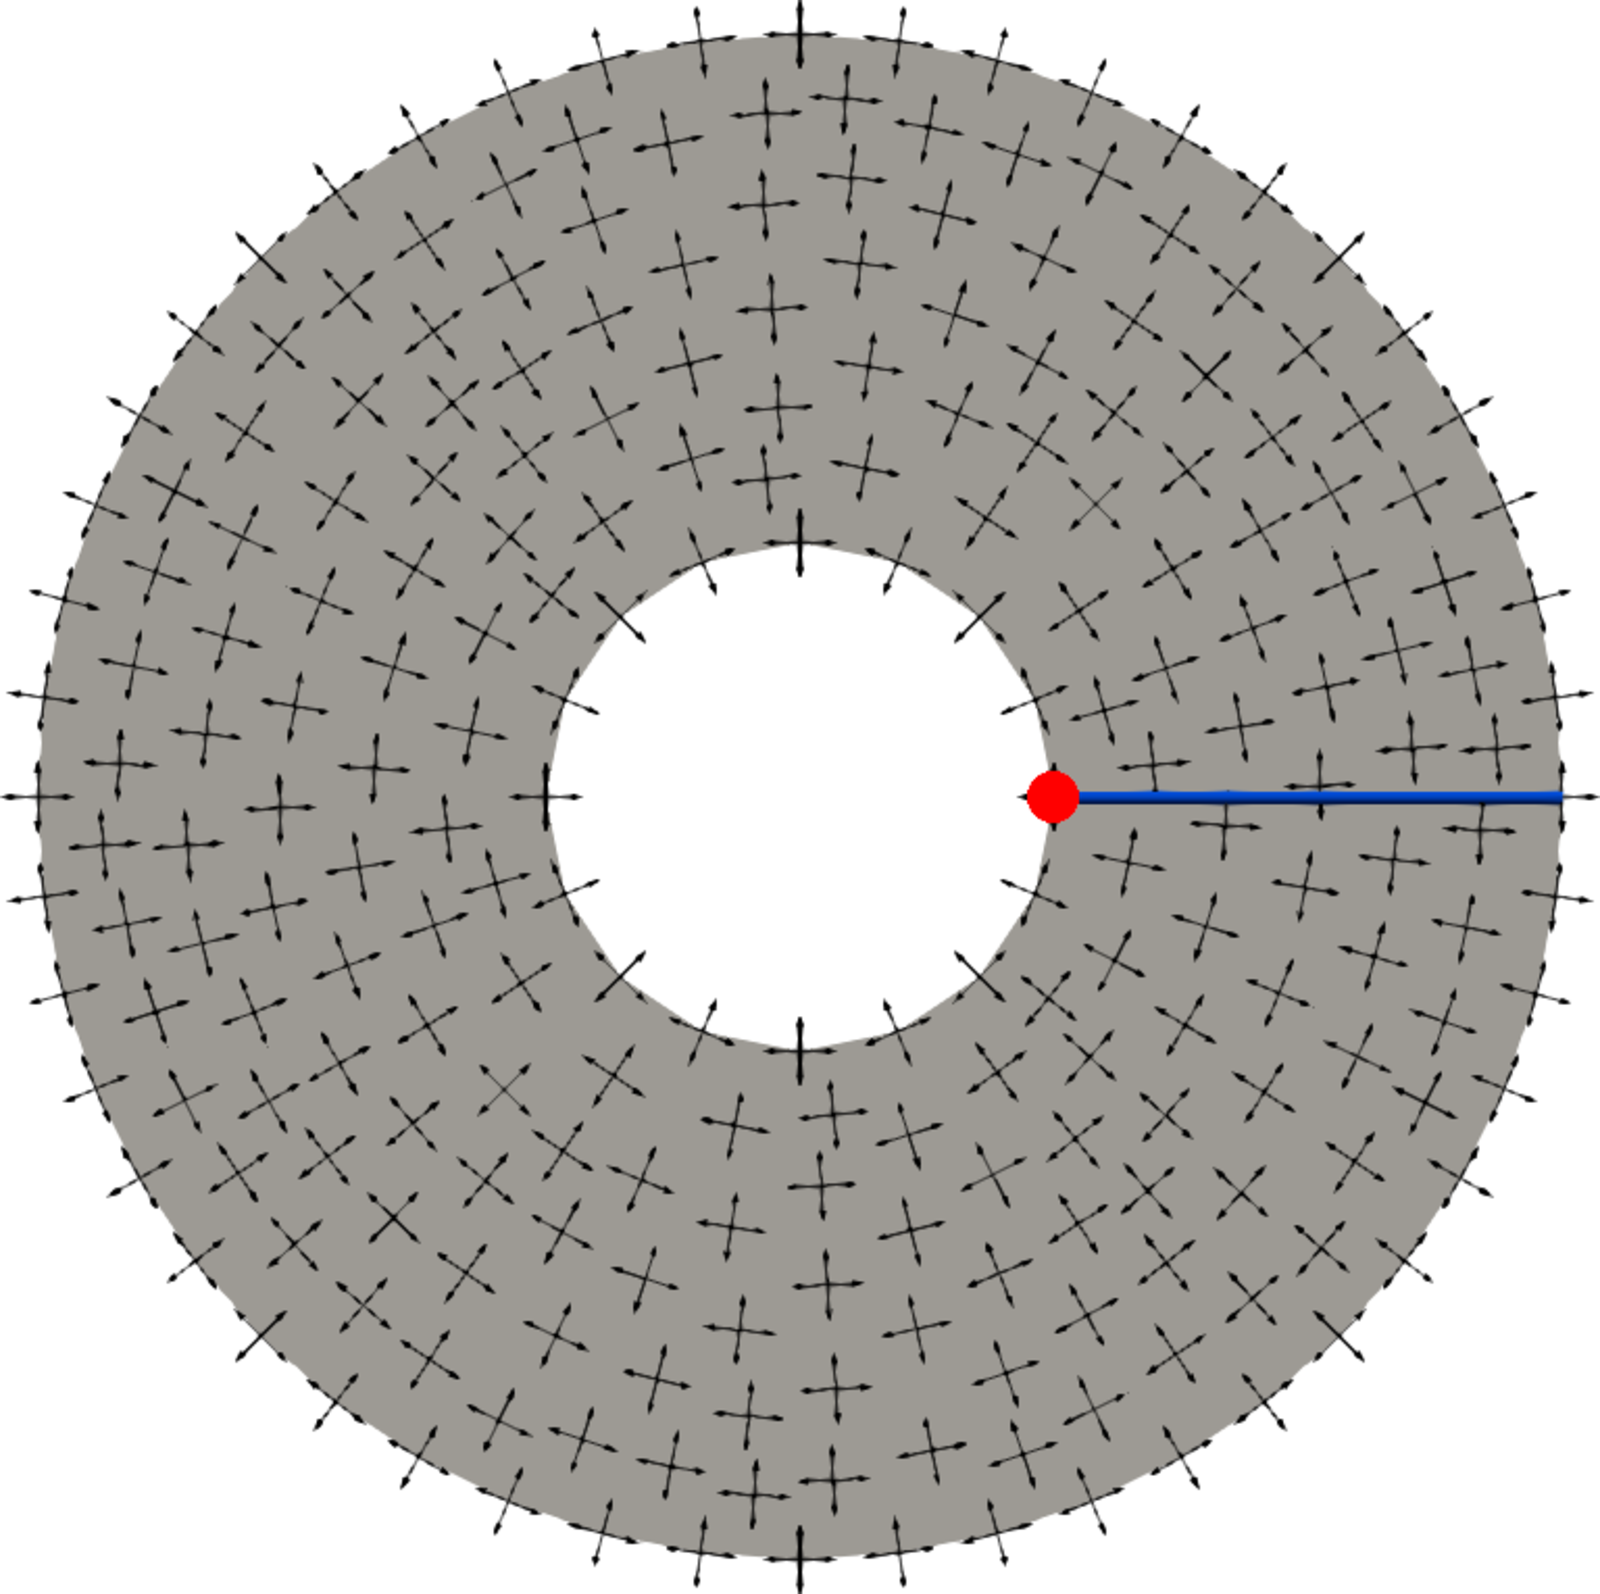
\includegraphics[scale=0.3]{images/anneau_cross.pdf}\hfill
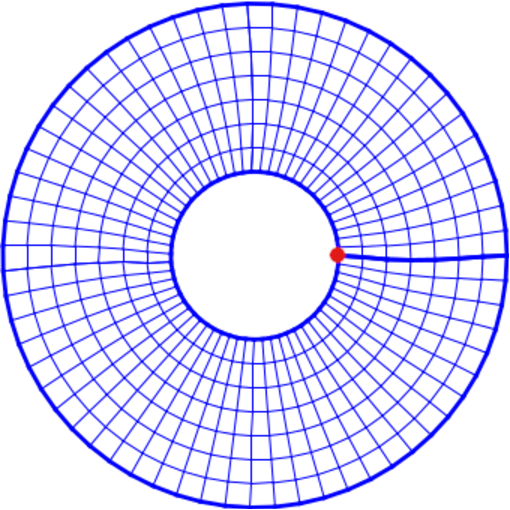
\includegraphics[scale=0.89]{images/anneau_mail.pdf}
\caption{Illustration du maillage quadrilatéral d'un anneau à partir d'un champ de croix radial.}
\label{fig:anneau}
\end{figure}

\subsection{Sur la conservation des propriétés du champ de croix initial}

À l'origine de notre travail, notre objectif principal était de générer des maillages quadrilatéraux pour des domaines en utilisant des champs de croix existants, tout en préservant leurs propriétés caractéristiques intrinsèques. Parmi ces caractéristiques, la forme globale du champ revêt une importance particulière. Par exemple, un champ de croix dérivé de la vitesse d'un fluide possède une forme spécifique à cet écoulement. La préservation de cette forme aurait permis d'obtenir des maillages alignés avec la dynamique fluide, offrant ainsi une adaptabilité aux propriétés physiques étudiées.

Malheureusement, notre méthode actuelle ne semble pas préserver efficacement cette caractéristique. L'approche que nous avons élaborée, basée sur l'alignement par un champ d'angle global du domaine, altère considérablement la forme du champ de croix initial. Cette altération ne permet pas de conserver les orientations spécifiques présentes dans le champ de croix initial. Cependant, notre méthode parvient à maintenir la localisation des points singuliers du champ de croix initial ainsi que leurs indices.

\subsection{Sur les singularités de bord}

Il est parfois obligatoire pour les simulations numériques de délimiter des parties de la frontière du domaine avec des nœuds physiques. C'est particulièrement le cas lors de l'application de conditions aux limites morcelées. Lorsque ces nœuds ne coïncident pas avec les nœuds géométriques (comme les coins), une manière de prendre en compte cette information serait de les considérer dans le champ de croix comme des points singuliers de bord.

La présence d'une singularité en bordure indique une rotation locale du champ de croix associée à la normale sortante. La quantification de cette rotation fournit la valeur de l'indice associé à la singularité (voir l'équation \eqref{eqn:Indexboundary}). Dans la littérature, les associations (angle de coin - indice) proposées tendent à minimiser la rotation du champ sur la frontière afin de maintenir le champ de croix à l'intérieur du domaine aussi lisse que possible. La distribution conventionnelle proposée dans la littérature correspond aux valeurs du tableau \ref{tabul} avec différentes tolérances autour des angles donnés (voir les détails dans \cite{macq2020ginzburg}).

\begin{table}[!h]
\centering
\begin{tabular}{|c|c|c|c|}
\hline
\multirow{2}{*}{angle} & \multirow{2}{*}{$\simeq\pi/2$} & \multirow{2}{*}{$\simeq\pi$} & \multirow{2}{*}{$\simeq3\pi/2$} \\
&&&\\
\hline
\multirow{2}{*}{index} & \multirow{2}{*}{$1/4$}   & \multirow{2}{*}{$0$}   & \multirow{2}{*}{$-1/4$}\\
&&&\\
\hline
\multirow{2}{*}{$N_s$} & \multirow{2}{*}{2}   & \multirow{2}{*}{3}   & \multirow{2}{*}{4}   \\
&&&\\
\hline
&&&\\
&&&\\
\multirow{2}{*}{Illustration} & \multirow{2}{*}{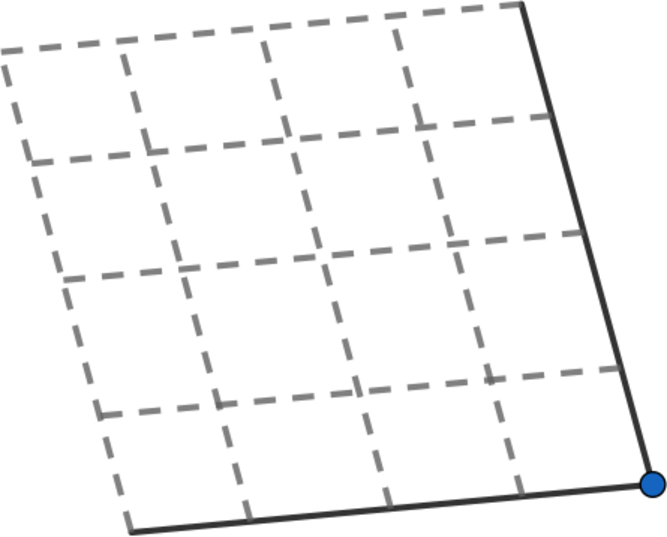
\includegraphics[scale=0.25]{images/geogebra-export_1.pdf}}   & \multirow{2}{*}{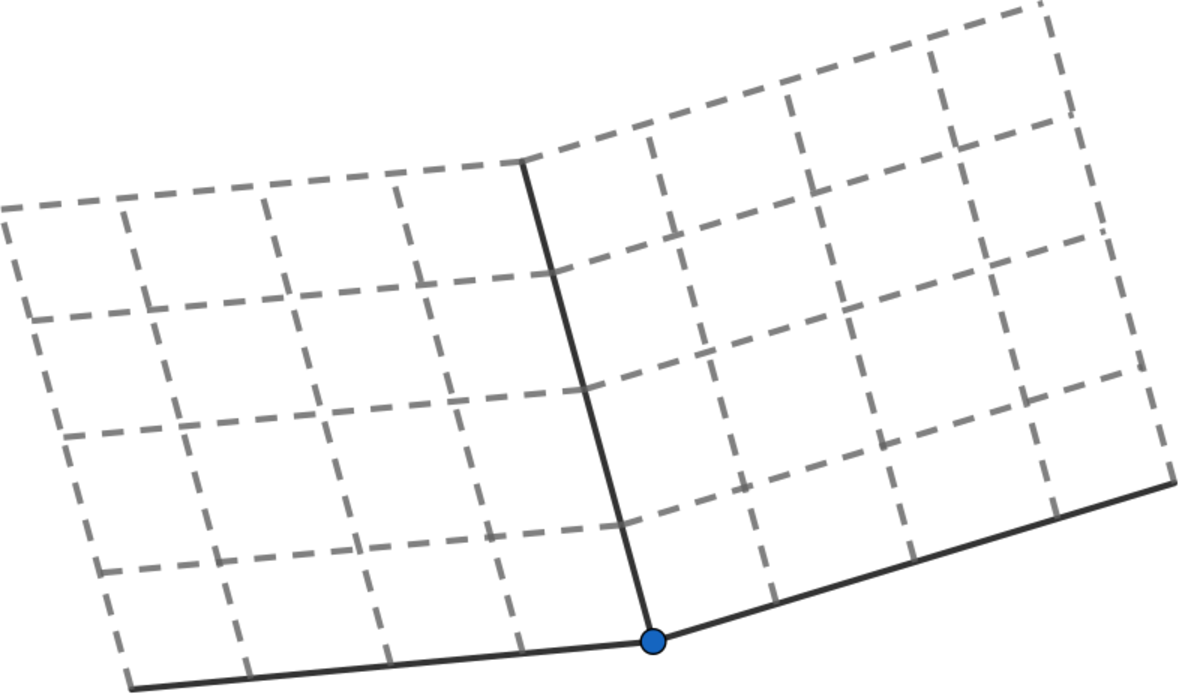
\includegraphics[scale=0.2]{images/geogebra-export_2.pdf}}   & \multirow{2}{*}{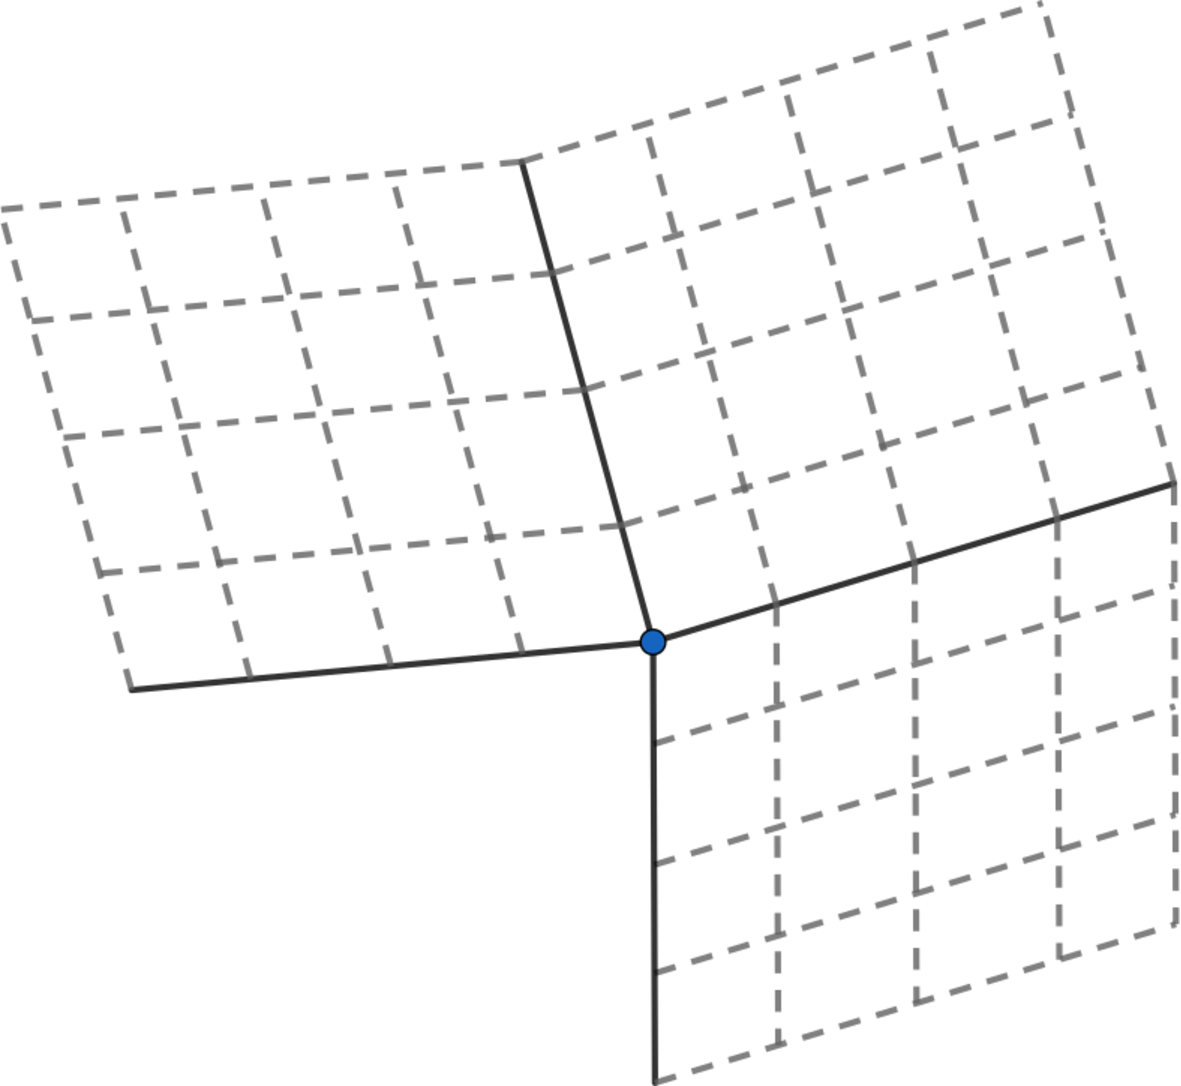
\includegraphics[scale=0.2]{images/geogebra-export_3.pdf}}   \\
&                          &                        &                           \\
&&&\\
&&&\\
&&&\\
&&&\\
&&&\\
&&&\\
&&&\\
\hline
\end{tabular}
\caption{Distribution usuelle d'angles-index de singularités de bord.}
\label{tabul}
\end{table}

Dans notre travail, nous gérons les points singuliers de bord lors de l'opération d'alignement du champ de croix initial par rapport au bord du domaine à mailler. Ces points sont spécifiés dans l'ensemble $\mathbf{B}$ et à chaque point $p\in\mathcal{B}$ est associé un paramètre $I_p$ représentant l'indice du point et donc son influence sur la rotation locale du champ. Cette approche offre la possibilité de définir, en un point quelconque du bord, un indice arbitraire, indépendemment de la valeur de l'angle formé par le bord au point considéré. Deux cas pratique peuvent être envisager pour la mise en oeuvre pratique de cette approche. Nous présentons ces deux possibilités sur les figures \ref{fig:demiDisc_sing_bord_first} et \ref{fig:demiDisc_sing_bord_second} \ref{fig:demiDisc_sing_bord_third}.

Sur la figure \ref{fig:demiDisc_sing_bord_first}, on se donne un champ de croix aligné le long du bord du domaine, comprenant trois points singuliers de bord d'indice $1/4$ et un point singulier interne d'indice $1/4$. Le maillage associé à ce champ de croix est également représenté sur cette figure. Ensuite, l'un des points singuliers de bord est déplacé en préservant son indice via l'opération d'alignement, comme illustré sur la figure \ref{fig:demiDisc_sing_bord_second}. Notons que puisque le champ de croix est déjà aligné par rapport au bord du domaine, le champ d'alignement utilisé dans cette opération est presque-partout nul.

Sur la figure \ref{fig:demiDisc_sing_bord_second}, le champ de croix initial présente trois points singuliers internes d'indice $1/4$, tandis que l'ensemble $\mathcal{B}$ est composé de trois points singuliers de bord d'indices $1/4$. Après l'opération d'alignement, le champ de croix final contient à la fois les singularités initialement présentes et celles spécifiées le long du bord du domaine via l'ensemble $\mathcal{B}$, comme illustré sur la figure \ref{fig:demiDisc_sing_bord_third}. Le maillage associé à ce champ de croix est également présenté sur cette figure.


\begin{figure}[!h]
\centering
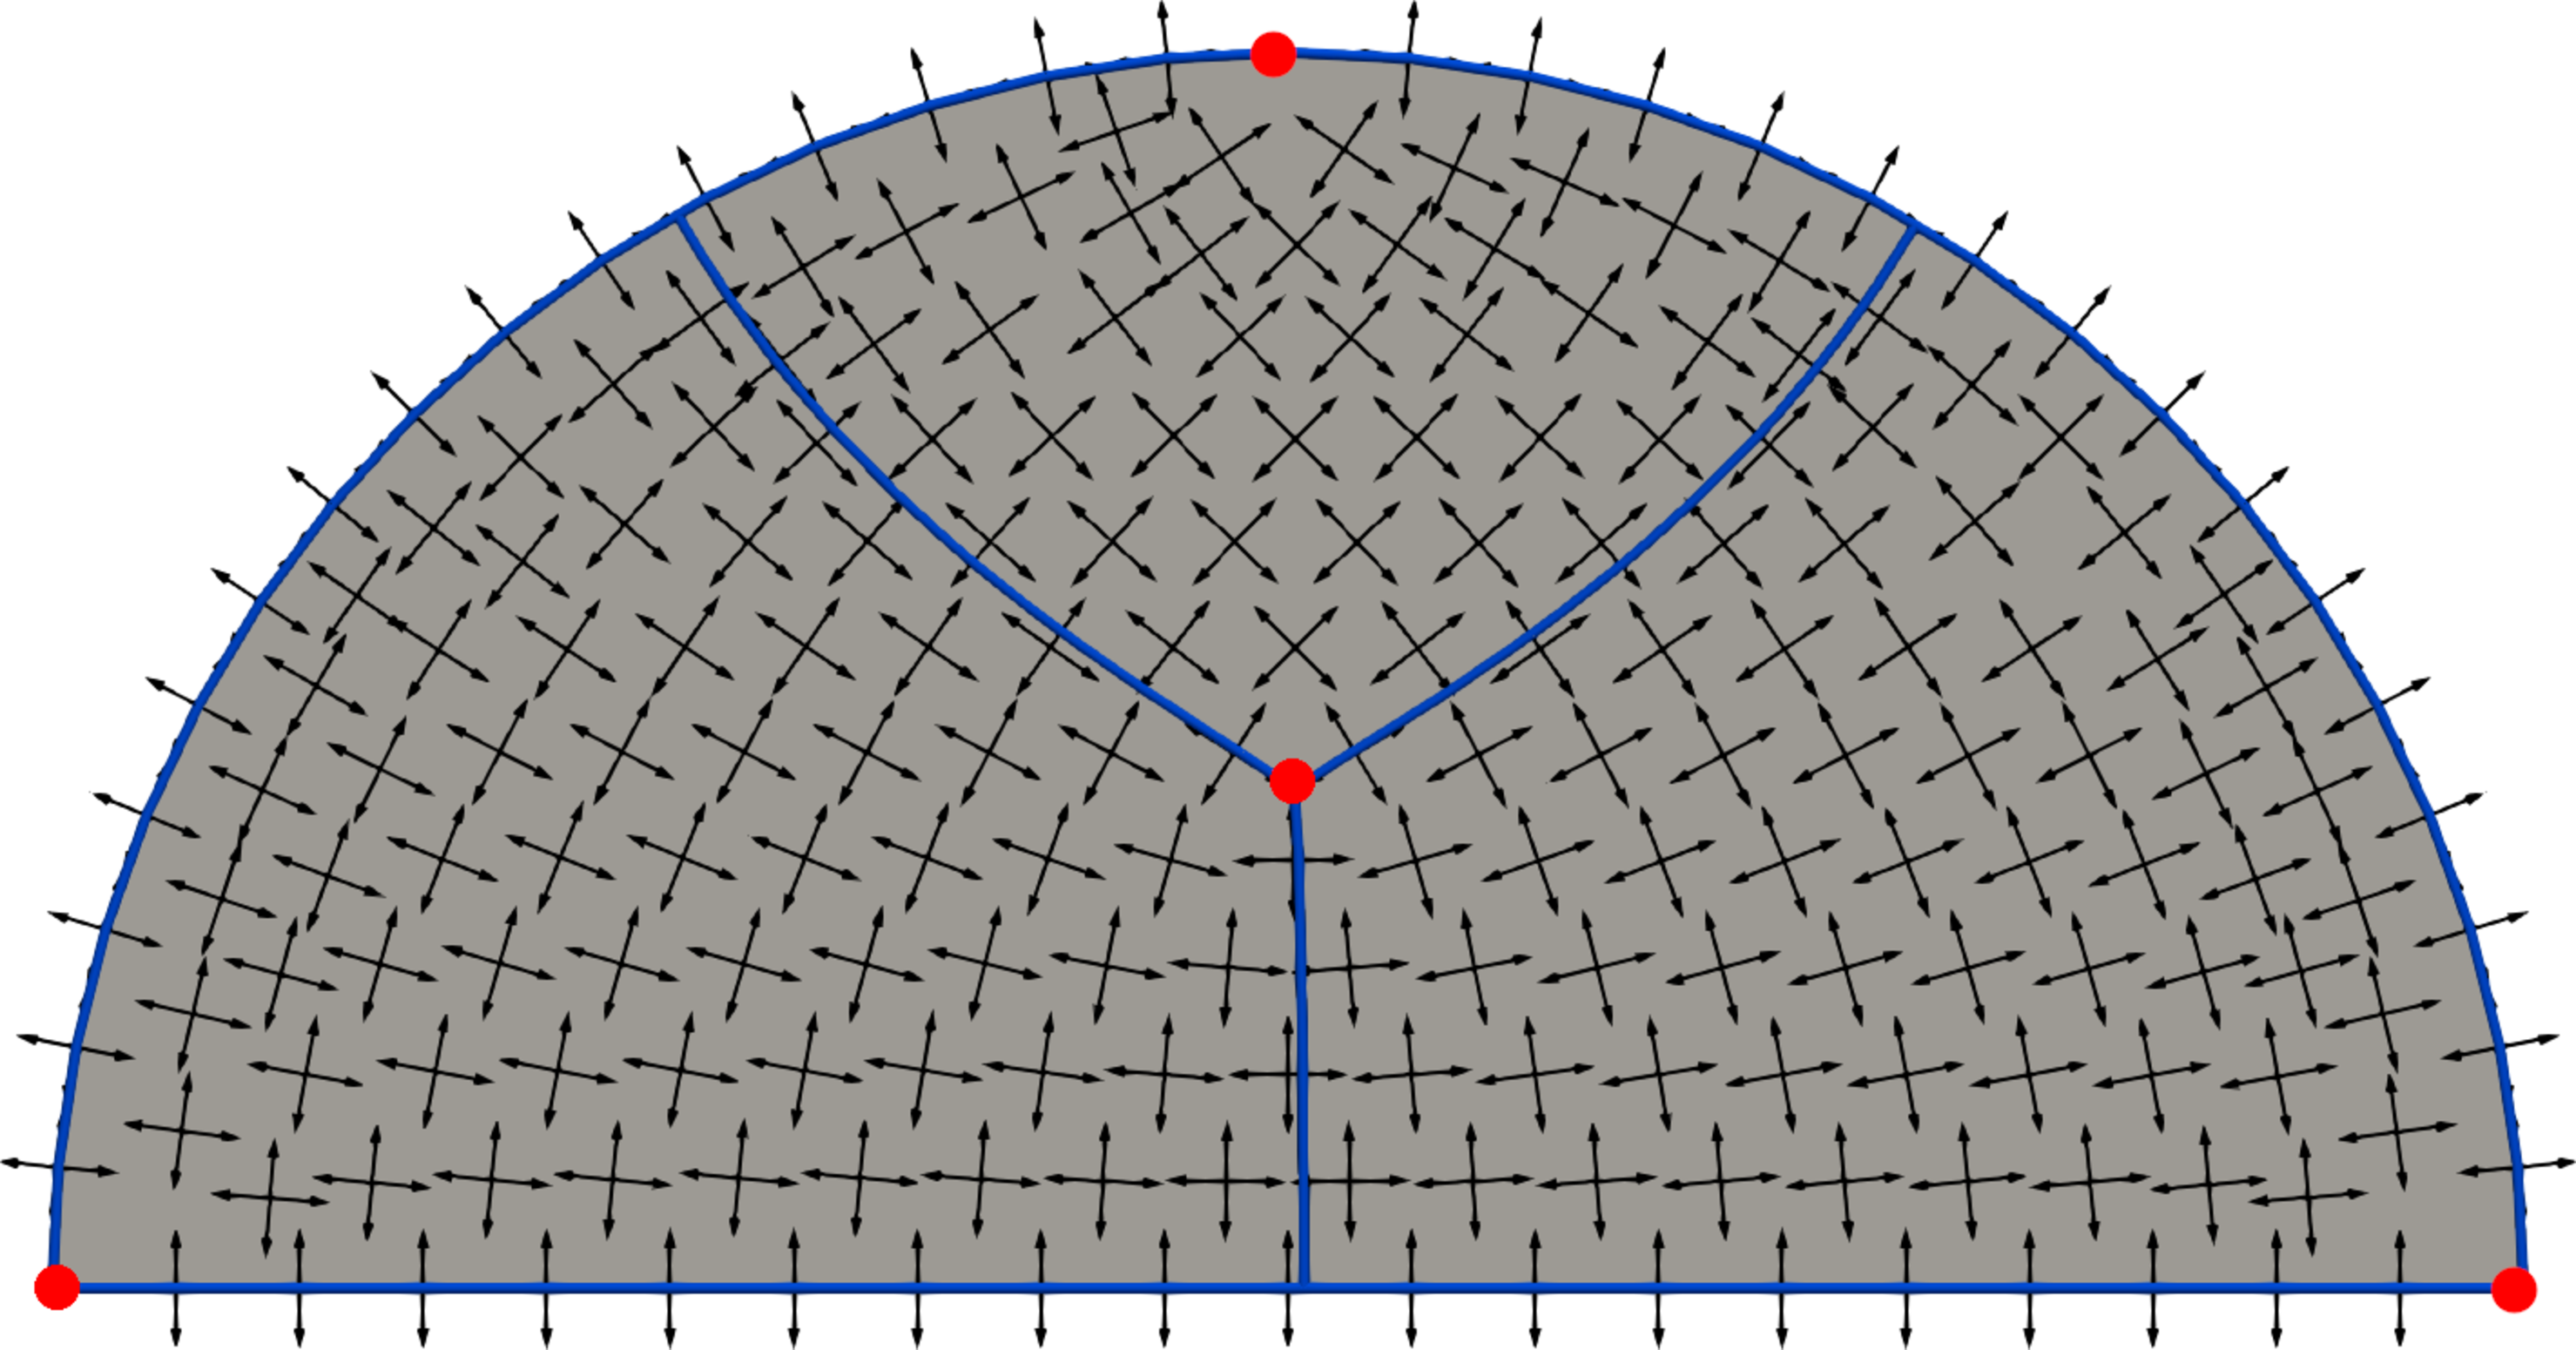
\includegraphics[scale=0.24]{images/yo_1.pdf}\\[0.5cm]
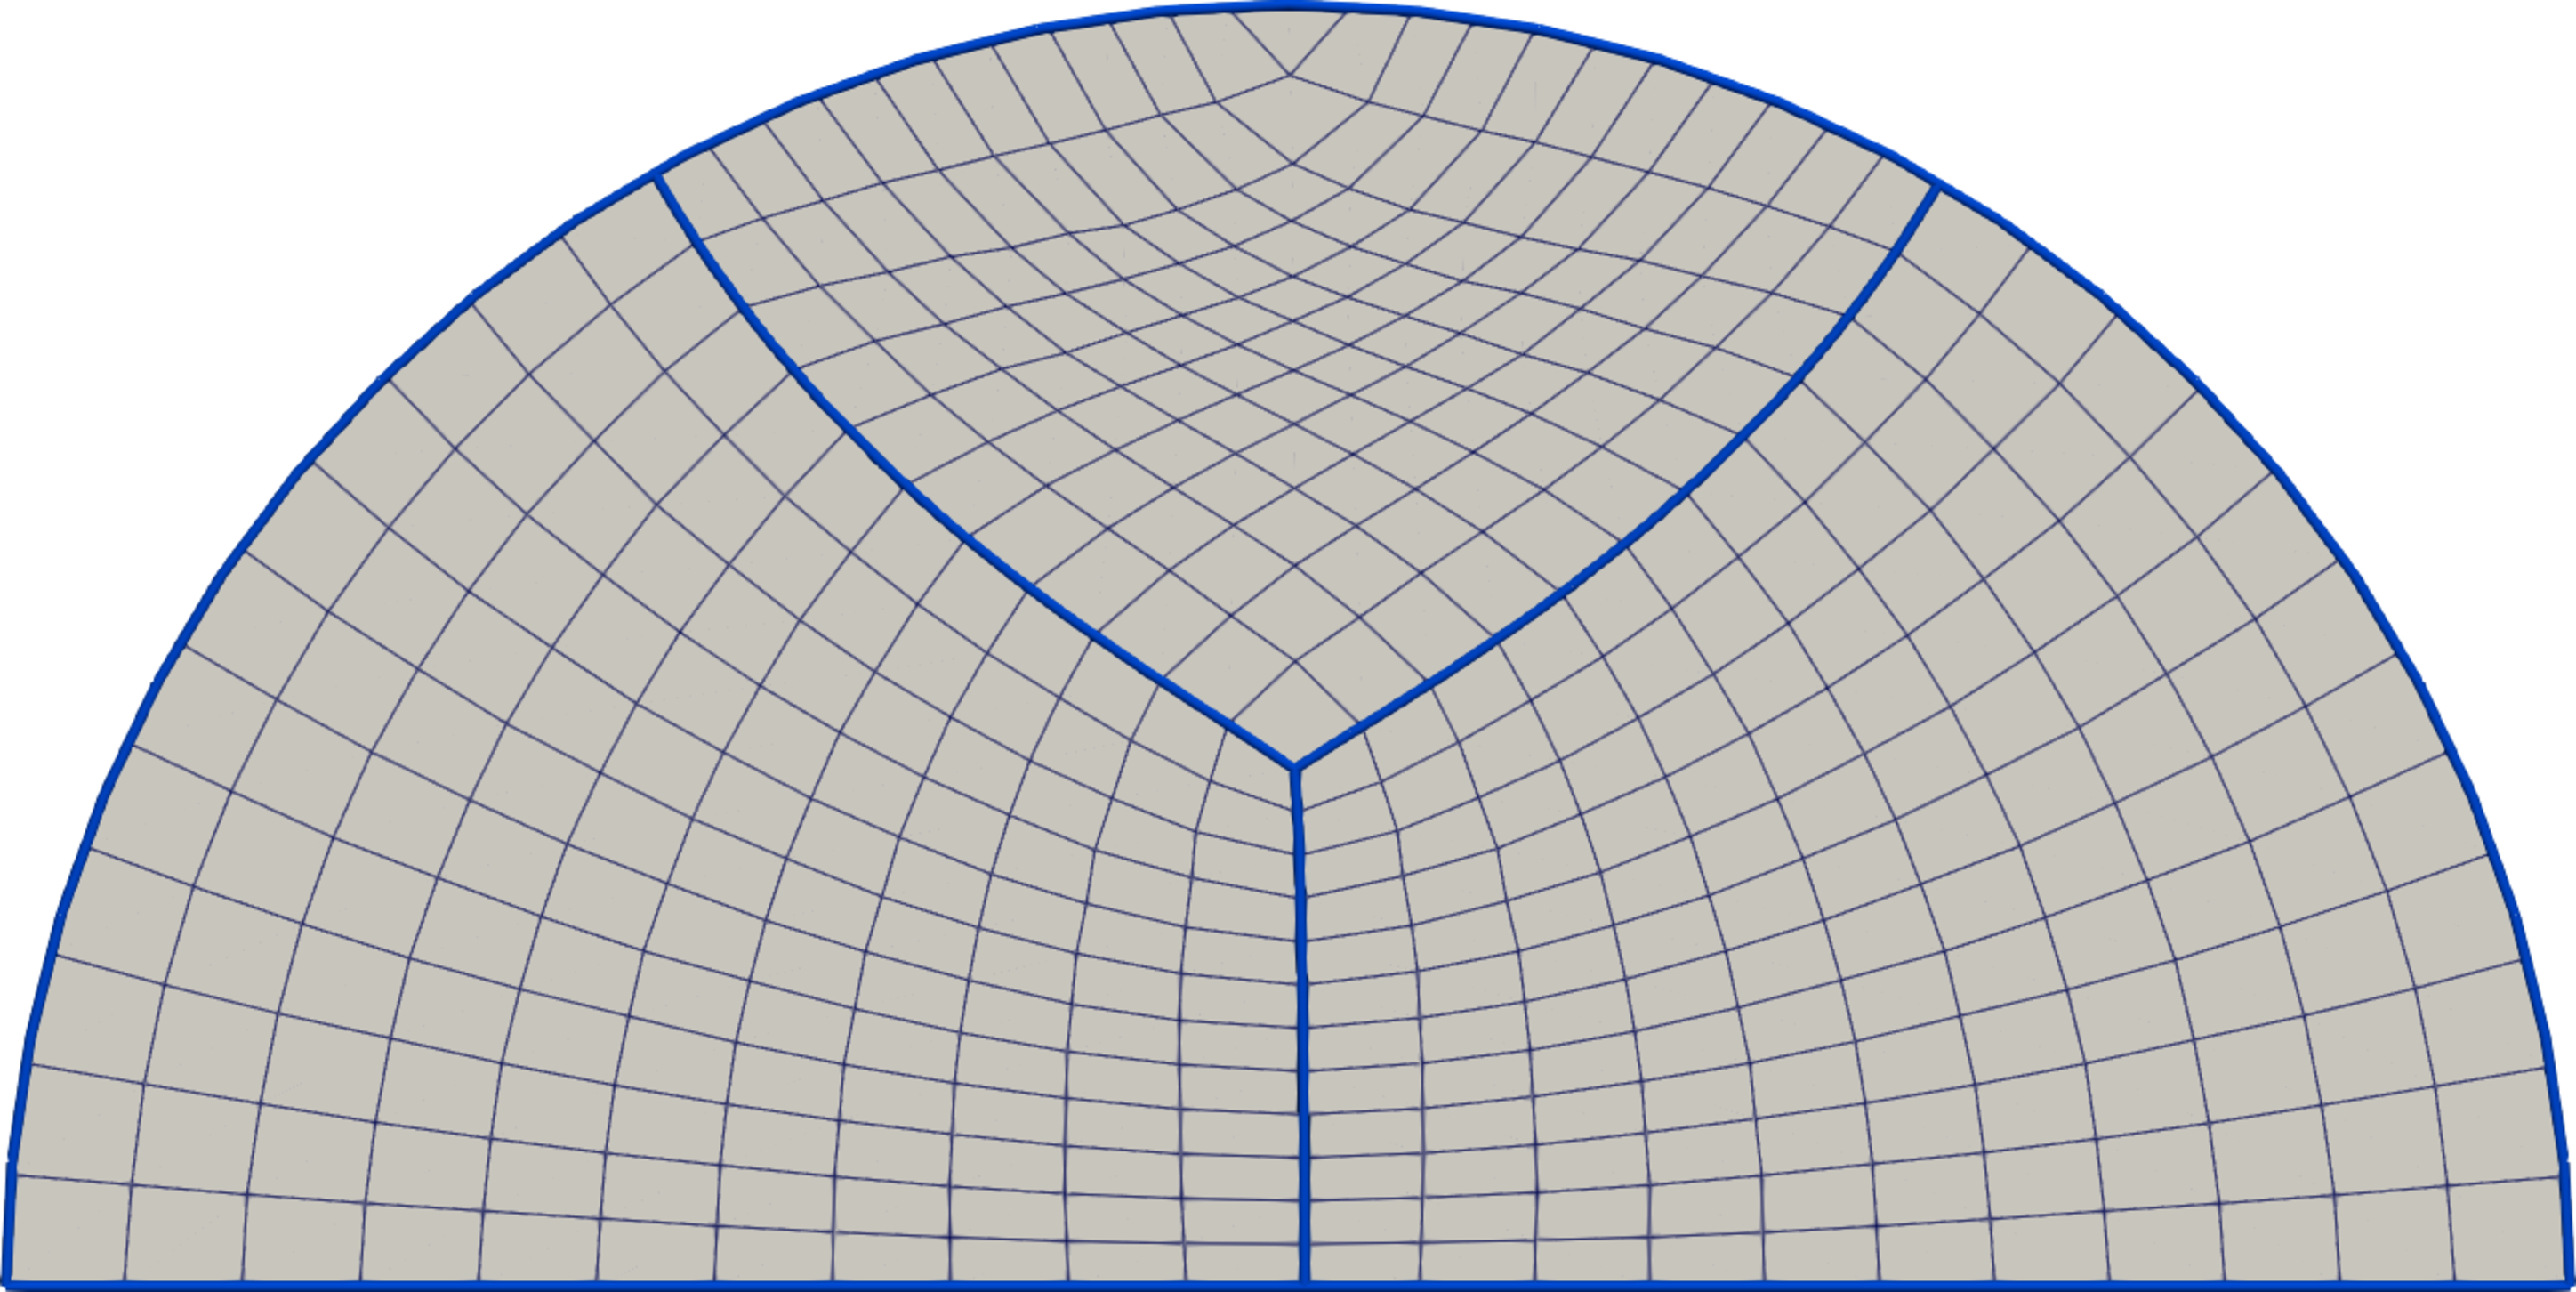
\includegraphics[scale=0.24]{images/yo_2.pdf}
\caption{Maillage du demi disque avec trois points singuliers d'indices $1/4$ sur le bord du domaine.}
\label{fig:demiDisc_sing_bord_first}
\end{figure}

\begin{figure}[!h]
\centering
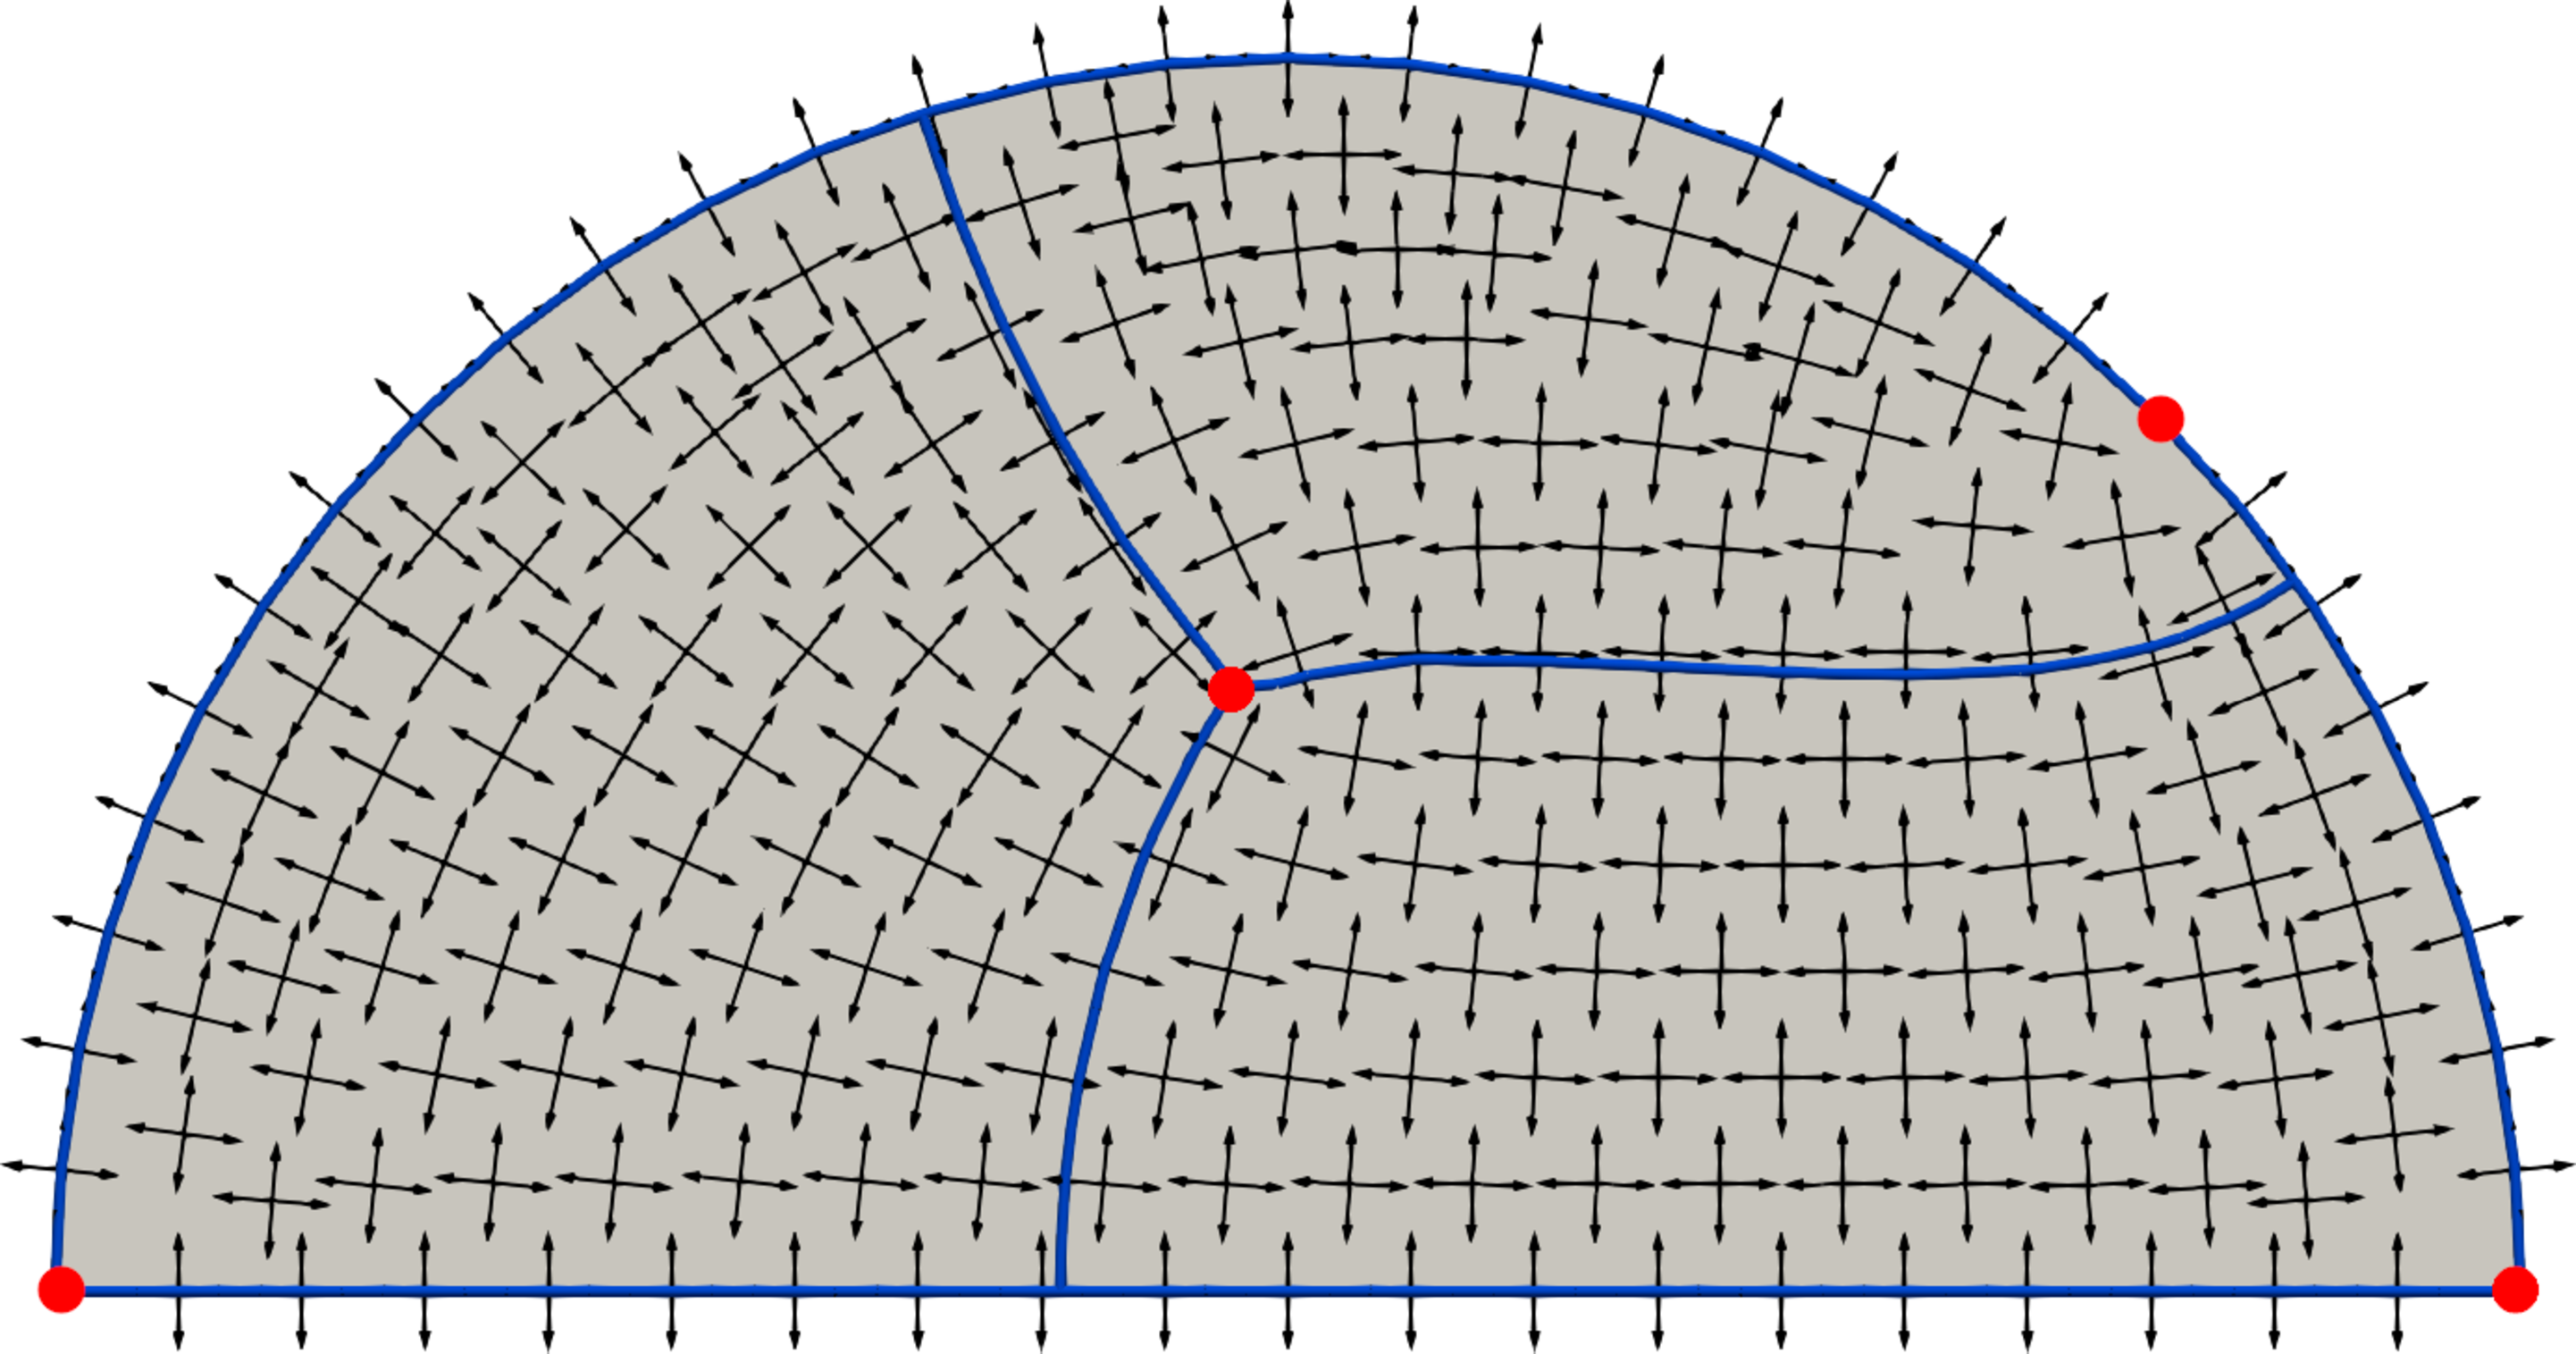
\includegraphics[scale=0.24]{images/yo_11.pdf}\\[0.5cm]
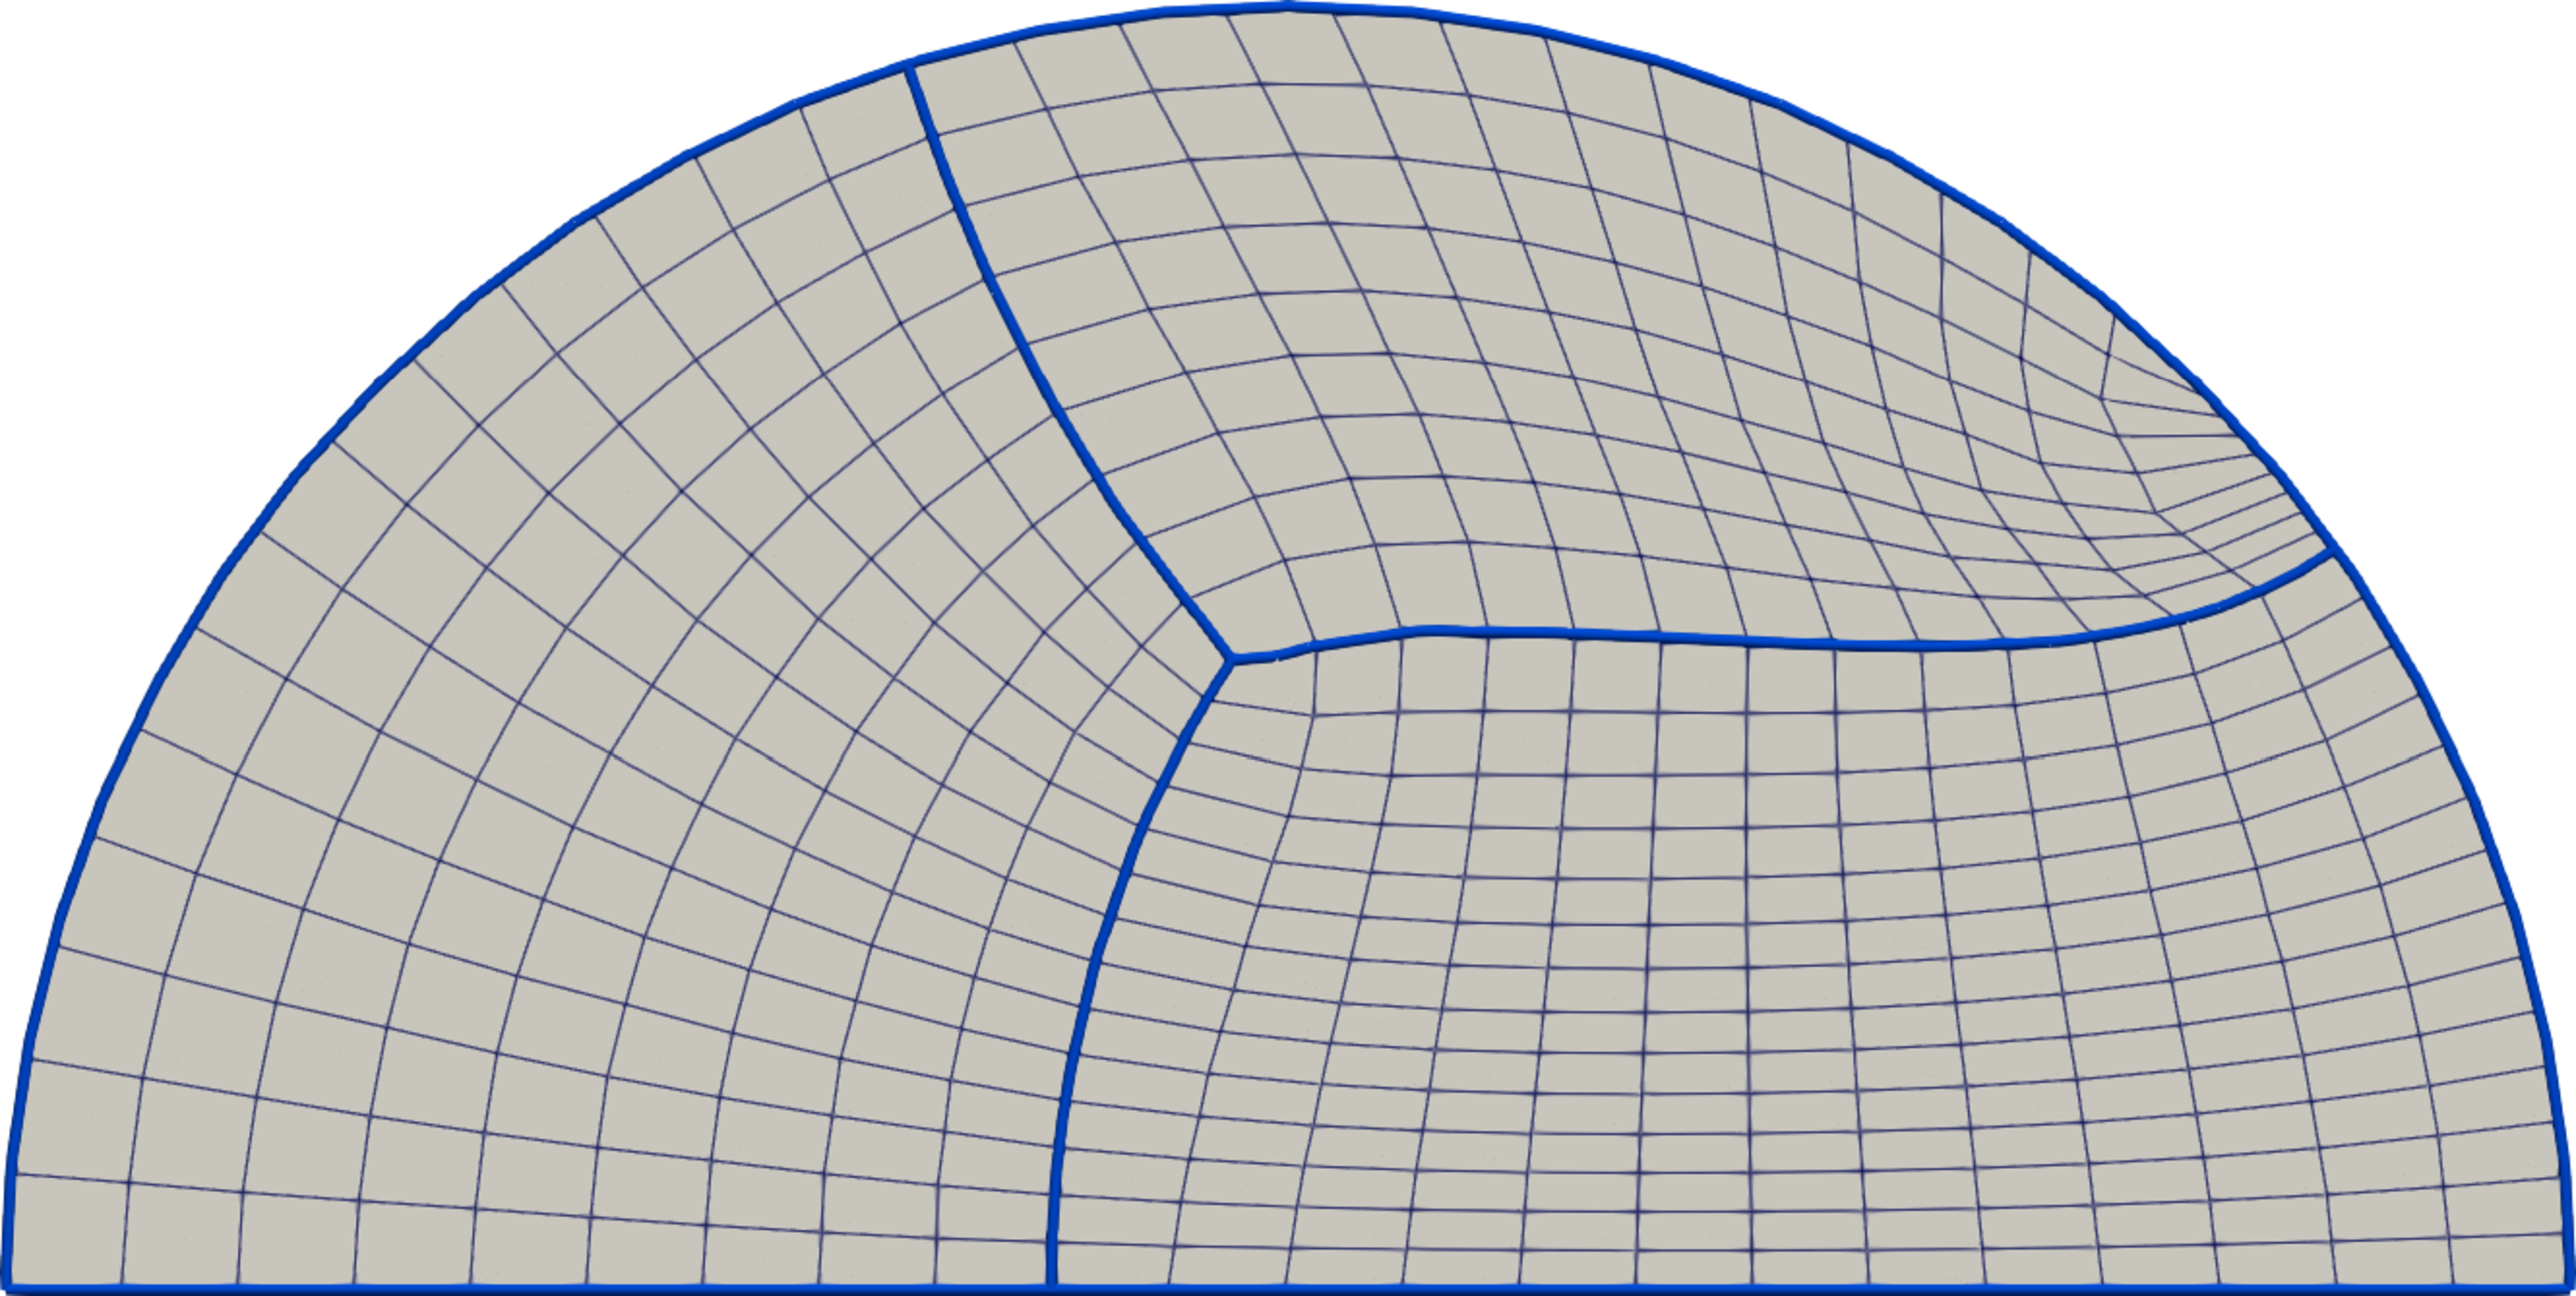
\includegraphics[scale=0.24]{images/yo_12.pdf}
\caption{Maillage du demi disque avec trois points singuliers d'indices $1/4$ sur le bord du domaine.}
\label{fig:demiDisc_sing_bord_second}
\end{figure}

\begin{figure}[!h]
\centering
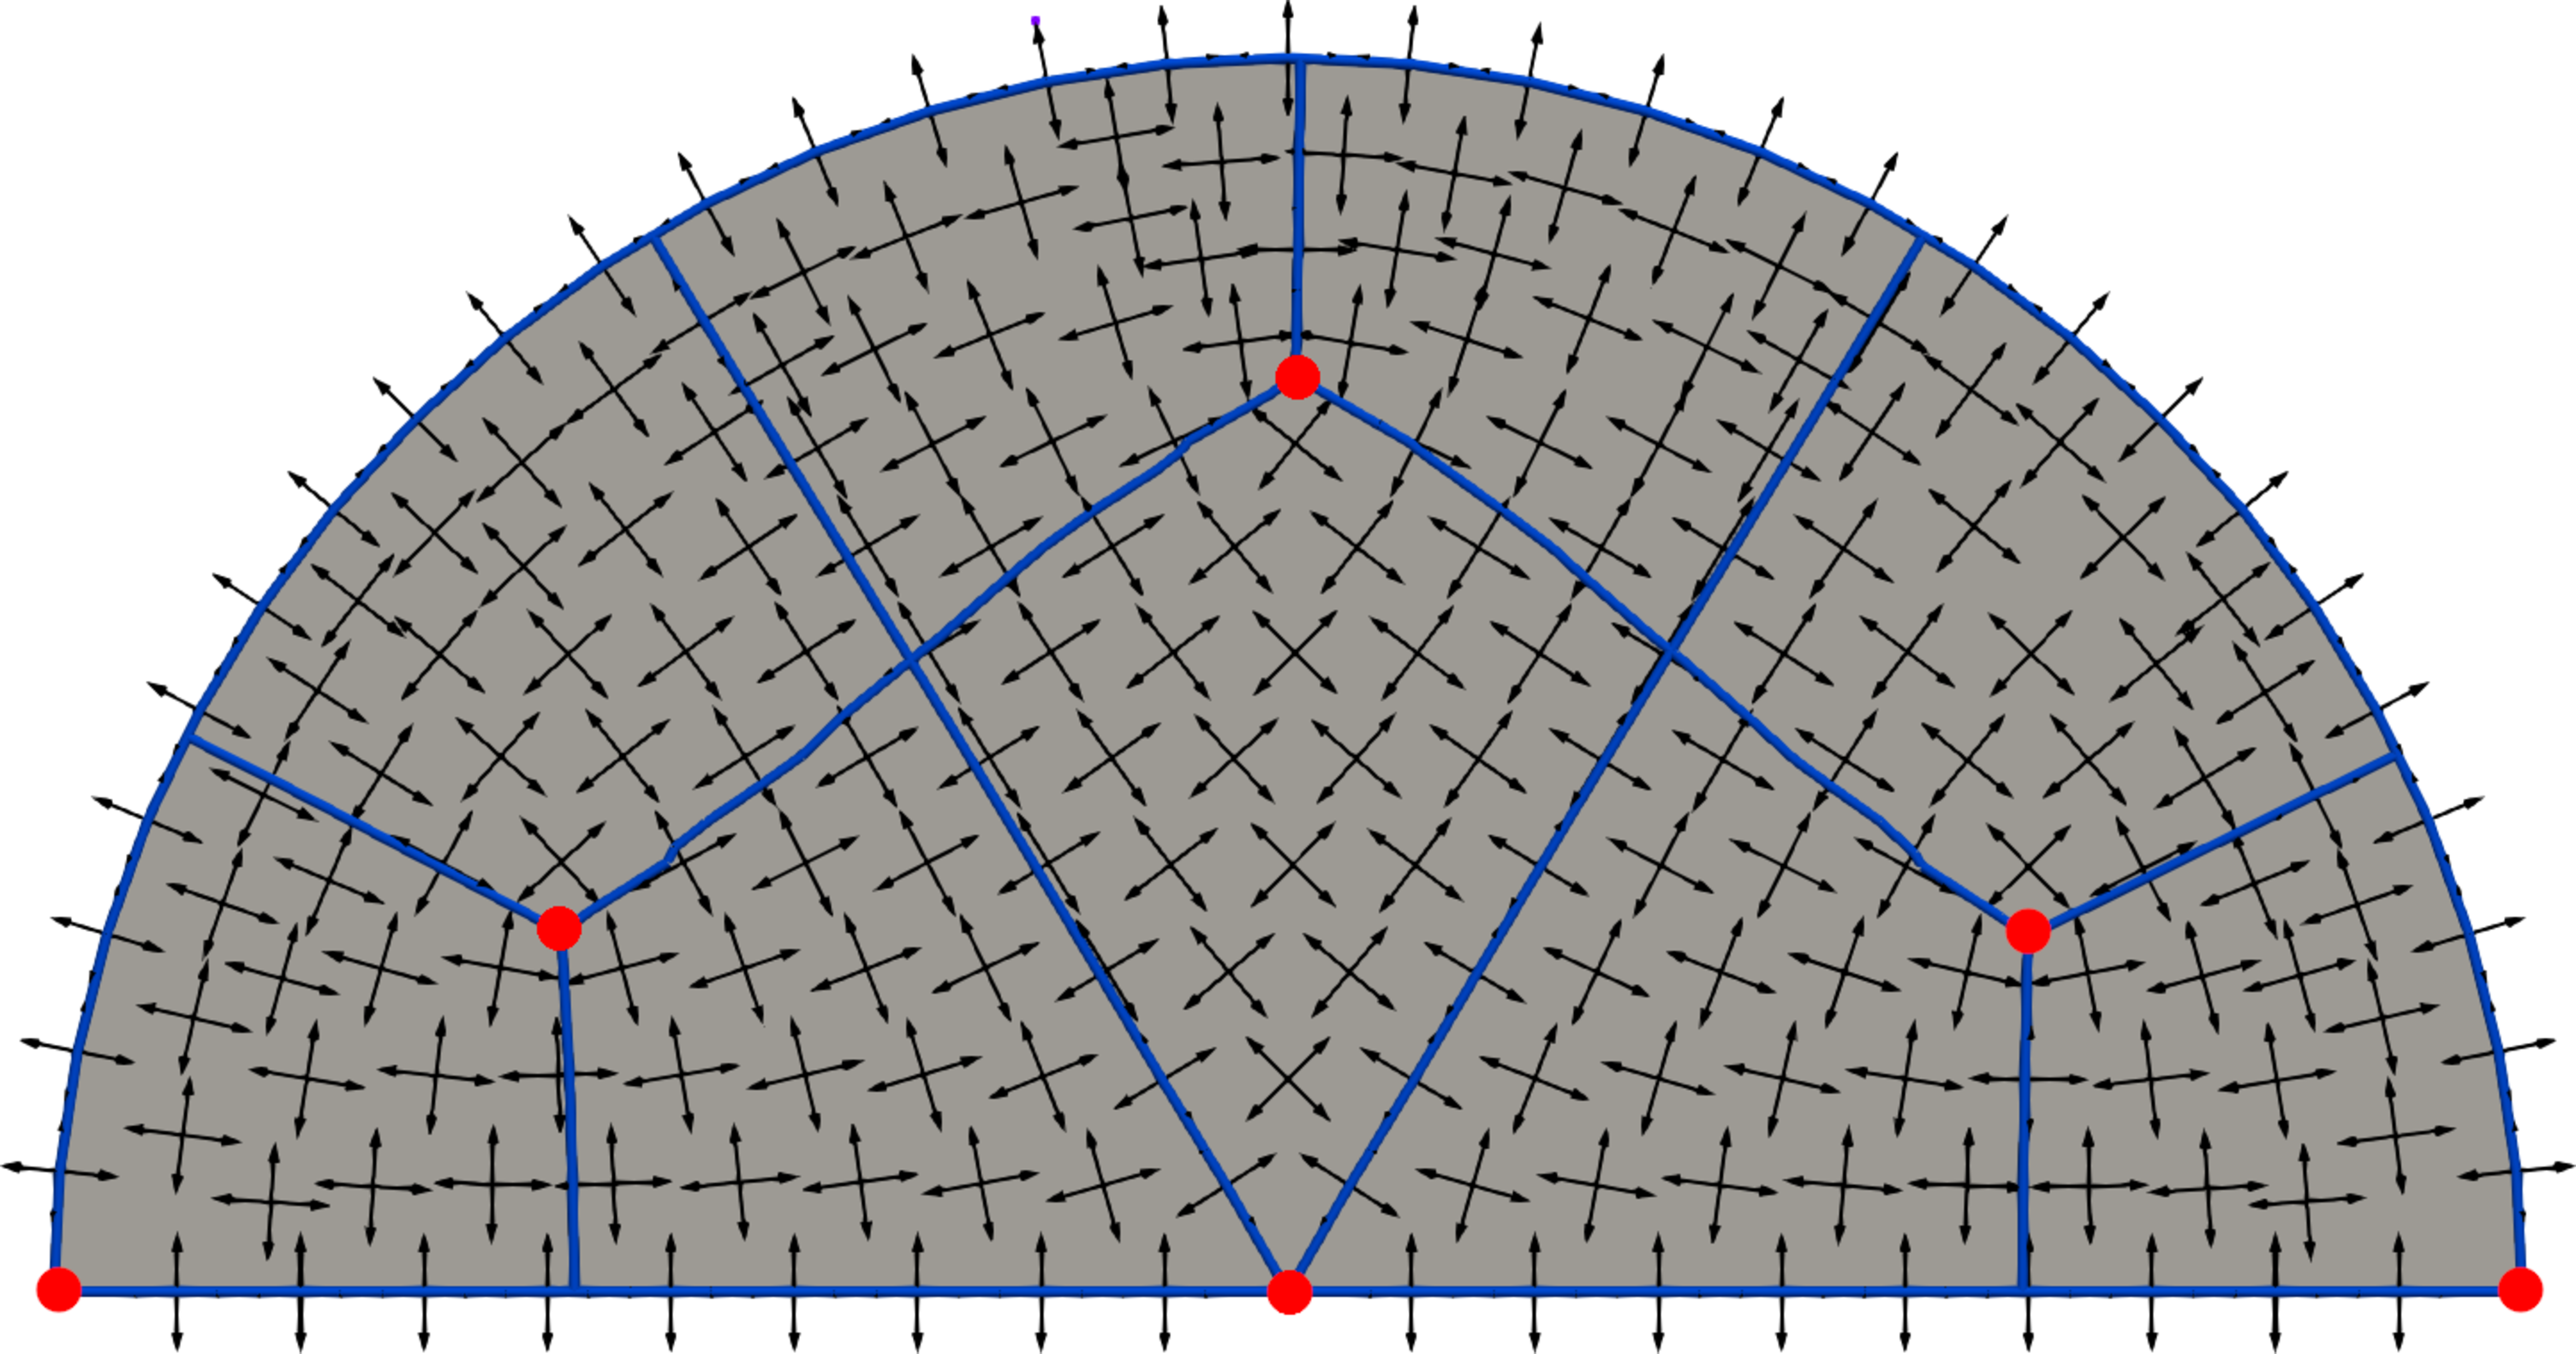
\includegraphics[scale=0.24]{images/yo_3.pdf}\\[0.5cm]
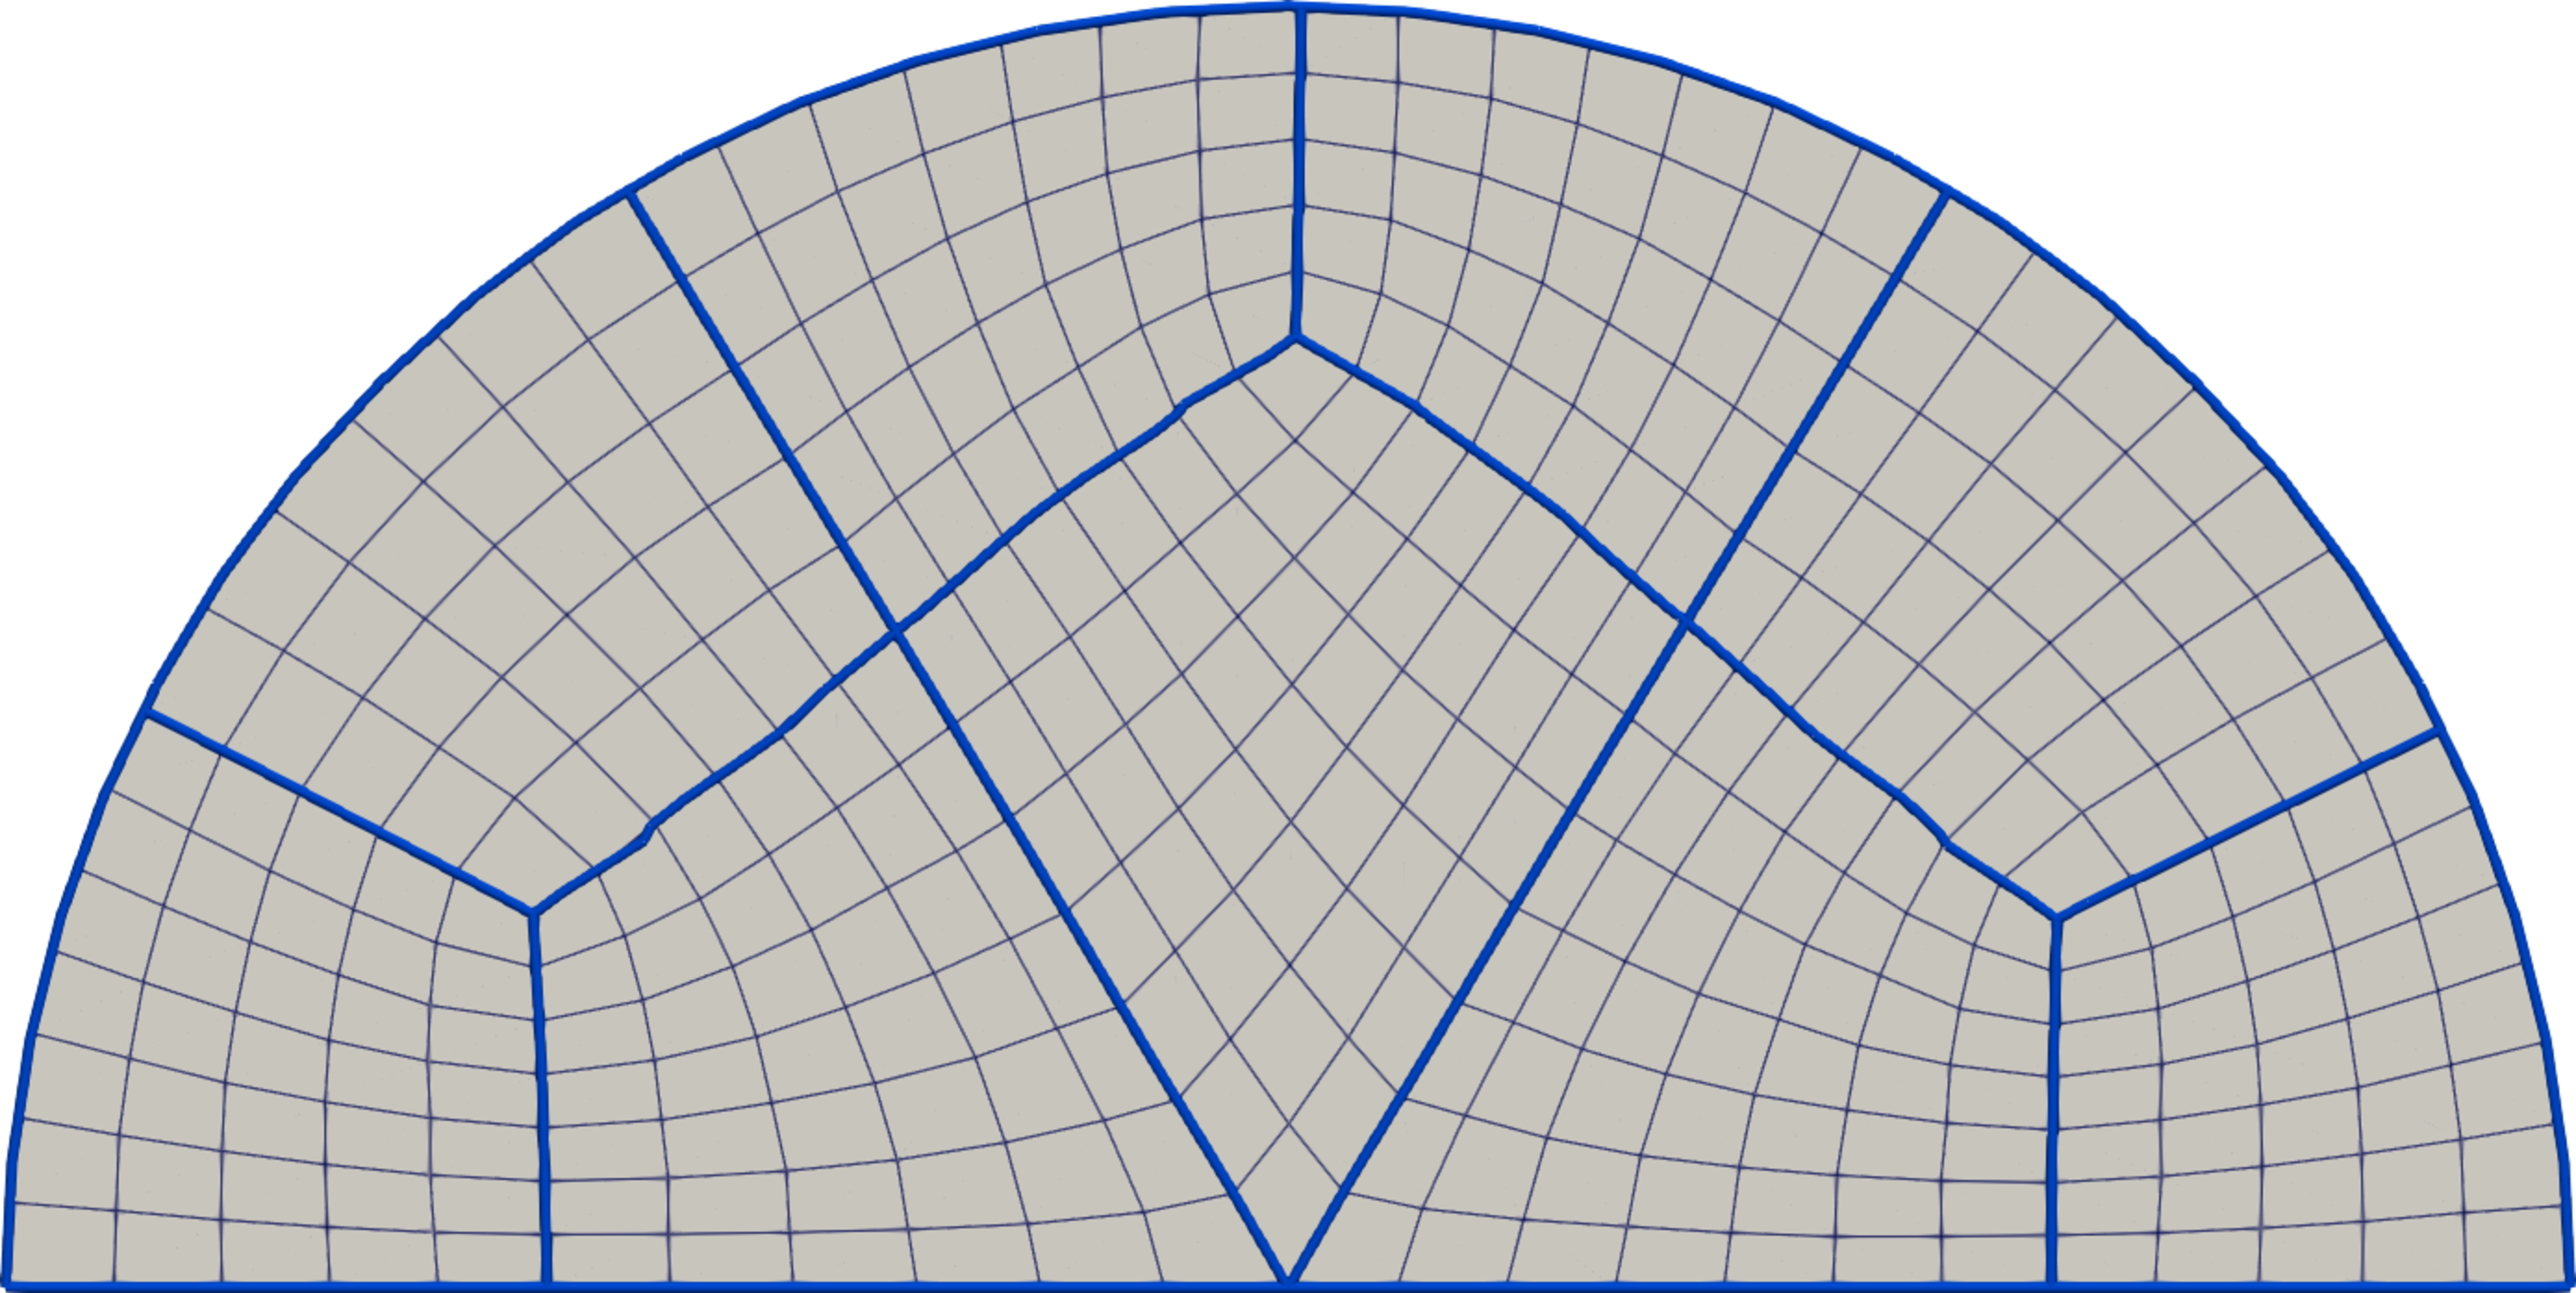
\includegraphics[scale=0.24]{images/yo_4.pdf}
\caption{Déplacement d'un point singulier sur le bord du domaine dans le champ de croix illustré sur la figure \ref{fig:demiDisc_sing_bord_second}.}
\label{fig:demiDisc_sing_bord_third}
\end{figure}

\begin{comment}
\begin{figure}[!h]
\centering
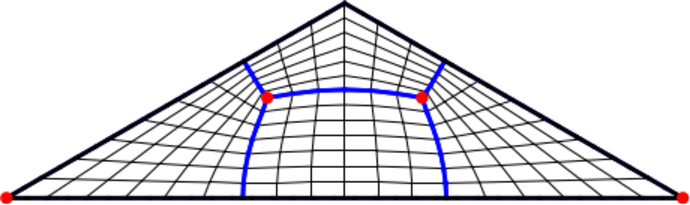
\includegraphics[scale=0.5]{images/mesh_quad_4.pdf}
%\caption{ Boundary (black), Separatrices (blue), Singularity (red) }
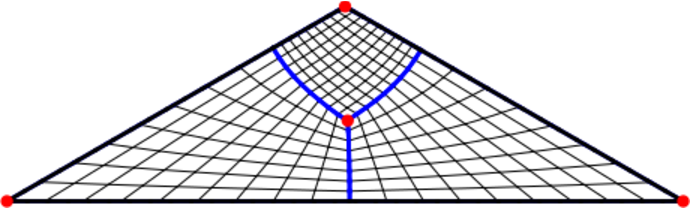
\includegraphics[scale=0.5]{images/mesh_quad_5.pdf}
\caption{En haut : 2 points singuliers internes d'indice 1/4 chacun et 2 points singuliers d'indice 1/4 sur la frontière, en bas : 1 point singulier interne d'indice 1/4 et 3 points singuliers d'indice 1/4 sur la frontière.}
\label{modeles_tri}
\end{figure}
\end{comment}


\subsection{Sur la construction du champ de correction}
La construction du champ de correction proposé dans la partie \ref{subsec:etude_de_la_methode} revient à trouvé un champ de croix $\bar{w}$ dont l'angle vérifie
\begin{equation}
    \left\{
    \begin{array}{lcll}
    \theta_{\bar{w}}^{\gamma_0}(1)-\theta_{\bar{w}}^{\gamma_0}(0)&=&\theta_{\bar{u}}^{\gamma_0}(0)-\theta_{\bar{u}}^{\gamma_0}(1)+2\pi\left(1-\displaystyle\sum_{p\in(\mathcal{B}\cup\mathcal{S}_{\bar{N}})\cap\Gamma_0}I_p\right)&\mbox{ sur }\Gamma_0\\\\
    \theta_{\bar{w}}^{\gamma_i}(1)-\theta_{\bar{w}}^{\gamma_i}(0)&=&\theta_{\bar{u}}^{\gamma_i}(0)-\theta_{\bar{u}}^{\gamma_i}(1)-2\pi\left(1+\displaystyle\sum_{p\in(\mathcal{B}\cup\mathcal{S}_{\bar{N}})\cap\Gamma_i}I_p\right)&\mbox{ sur }\Gamma_i,\\\\
    &&&~\forall i\in\llbracket 1, n_b-1\rrbracket.
    \end{array}
    \right.
    \label{eqn:disc_hypothese_w}
\end{equation}
Pour construire un tel champ de croix, nous proposons plusieurs options. La première consiste a calculer le champ d'angle $\varphi$ vérifiant l'equation suivante:
\begin{equation}
\left\{
\begin{array}{lcll}
    \Delta\varphi &=& 0 & \mbox{ dans }\Omega,\\\\
    \displaystyle\frac{1}{2\pi}\displaystyle\int_{\Gamma_0}d\varphi &=& \theta_{\bar{u}}^{\gamma_0}(0)-\theta_{\bar{u}}^{\gamma_0}(1)+2\pi\left(1-\displaystyle\sum_{p\in(\mathcal{B}\cup\mathcal{S}_{\bar{N}})\cap\Gamma_0}I_p\right)&\mbox{ sur }\Gamma_0\\\\
    \displaystyle\frac{1}{2\pi}\displaystyle\int_{\Gamma_i}d\varphi &=& \theta_{\bar{u}}^{\gamma_i}(0)-\theta_{\bar{u}}^{\gamma_i}(1)-2\pi\left(1+\displaystyle\sum_{p\in(\mathcal{B}\cup\mathcal{S}_{\bar{N}})\cap\Gamma_i}I_p\right)&\mbox{ sur }\Gamma_i,\\\\
    &&&~\forall i\in\llbracket 1, n_b-1\rrbracket.
\end{array}
\right.
\end{equation}
Le champ de croix $\bar{w}$ est alors formé en utilisant le champ d'angle $\theta_{\bar{w}}(p)=\varphi(p)$ pour tout $p\in\Omega$. Néanmoins, cette méthode induit l'émergence de points singuliers aux frontières dans le champ de croix $\bar{w}$. Par conséquent, cela va engendrer l'apparition de points singuliers non souhaités aux frontières du champ de croix $\bar{v}$ (résultant de l'alignement), et par extension, le risque de créer des quadrilatères dégénérés lors de la génération du maillage quadrilatéral pour le domaine.

Une autre alternative pour construire le champ de croix $\bar{w}$ consiste à calculer le champ de vecteur $h$ vérifiant

\begin{equation}
\left\{
\begin{array}{lcll}
    \Delta h &=& 0 & \mbox{ dans }\Omega,\\\\
    \displaystyle\frac{1}{2\pi}\displaystyle\int_{\Gamma_0}d\theta_{h} &=&4\left[\theta_{\bar{u}}^{\gamma_0}(0)-\theta_{\bar{u}}^{\gamma_0}(1)+2\pi\left(1-\displaystyle\sum_{p\in(\mathcal{B}\cup\mathcal{S}_{\bar{N}})\cap\Gamma_0}I_p\right)\right]&\mbox{ sur }\Gamma_0\\\\
    \displaystyle\frac{1}{2\pi}\displaystyle\int_{\Gamma_i}d\theta_{h} &=& 4\left[\theta_{\bar{u}}^{\gamma_i}(0)-\theta_{\bar{u}}^{\gamma_i}(1)-2\pi\left(1+\displaystyle\sum_{p\in(\mathcal{B}\cup\mathcal{S}_{\bar{N}})\cap\Gamma_i}I_p\right)\right]&\mbox{ sur }\Gamma_i,\\\\
    &&&~\forall i\in\llbracket 1, n_b-1\rrbracket.
\end{array}
\right.
\label{eqn:disc_lefeu_1}
\end{equation}
Noter qu'en fonction du choix du $\theta_h$ sur le bord (en accord avec les condition de bord de l'équation \ref{eqn:disc_lefeu_1}) on obtiendra différent champ de vecteur ayant tous la particularité de ne présenté aucun point singulier sur le bord du domaine. On peut ensuite construire le champ de croix $\bar{w}$ via la formule suivante:
\begin{equation}
    \bar{w}(p) =
\left\{
    \begin{array}{ll}
        \displaystyle\left\{\mathbf{R}\left(\frac{m\pi}{2}\right)\mathbf{R}\left(\frac{\theta_h(p)}{4}\right)(1, 0)^t,~ m\in \mathbb{Z}\right\} &\text{ si }h(p)\neq 0,\\\\
        0& \text{sinon}.
    \end{array}
\right.
\label{eqn:disc_repr_to_cross}
\end{equation}

Une dernière possibilité consiste à résoudre directement l'équation vectorielle suivante.

\begin{equation}
\left\{
\begin{array}{lcll}
    \Delta h &=& 0 & \mbox{ dans }\Omega,\\\\
    h(p) &=&
    \left\{
    \begin{array}{ll}
        \mathbf{R}\displaystyle\left(4(\theta_{\bar{N}}(p)-\theta_{\bar{u}}(p))\right)(1, 0)^t &\text{ si }\bar{N}(p)\neq 0\mbox{ et }\bar{u}(p)\neq 0\\\\
        0& \text{sinon}
    \end{array}
    \right.
    &\mbox{ sur }\partial\Omega.\\\\
\end{array}
\right.
\label{eqn:disc_lefeu_2}
\end{equation}
Le champ de croix $\bar{w}$ est ensuite construit comme dans le cas précédent grace à la formule \ref{eqn:disc_repr_to_cross}.

\begin{remark}
Les deux dernières alternatives présentées peuvent potentiellement introduire de nouveaux points singuliers internes dans le champ de croix final.
\end{remark}


\subsection{Sur les multi-matériaux}

Formellement, un multi-matériau correspond à l'ensemble de plusieurs sous-domaines (matériaux) connexe, délimités par leurs frontières respectives. La gestion de telles géométries implique un traitement localisé de chaque sous-domaine. Cependant, il est crucial de prendre en considération les jonctions singulières entre ces divers sous-domaines. Par exemple, dans la figure \ref{connexe3}, la géométrie est constituée d'une combinaison de deux demi-disques et d'une plaque carrée avec un trou circulaire. Le maillage de chacun des sous-domaines peut être réalisé aisément grâce aux techniques présentées précédemment. Toutefois, il est impératif de prendre en compte les points de jonction entre les trois sous-domaines. Sans cela, certaines régions formées ne présenteront pas quatre côtés dans l'assemblage final.

\begin{figure}[!h]
\centering
\includegraphics[scale=0.535]{images/carreDiscPleinCouper domain.pdf}\hfill
\includegraphics[scale=0.8]{images/mesh_quad_6.pdf}
\caption{Un exemple de géométrie multi-matériaux. Gauche: Domaine, droite: maillage quadrilatéral.}
\label{connexe3}
\end{figure}


%%% Local Variables:
%%% mode: latex
%%% TeX-master: "../phdthesis"
%%% End:

